%% ----------------------------------------------------------------
%% Thesis.tex -- MAIN FILE (the one that you compile with LaTeX)
%% ---------------------------------------------------------------- 
% Set up the document
\documentclass[a4paper, 11pt, twoside]{Thesis}  % Use the "Thesis" style, based on the ECS Thesis style by Steve Gunn

\graphicspath{ {Figures/} }  % Location of the graphics files (set up for graphics to be in PDF format)

% Include any extra LaTeX packages required
% \usepackage[square, numbers, comma, sort&compress]{natbib}  % Use the "Natbib" style for the references in the Bibliography
\usepackage{verbatim}  % Needed for the "comment" environment to make LaTeX comments
\usepackage{vector}  % Allows "\bvec{}" and "\buvec{}" for "blackboard" style bold vectors in maths
\hypersetup{urlcolor=blue, colorlinks=true}  % Colours hyperlinks in blue, but this can be distracting if there are many links.
\usepackage{apalike}
\usepackage[round]{natbib}
\bibliographystyle{plainnat}
\usepackage{lipsum}
\usepackage{textcomp}
\usepackage{enumerate}
\usepackage{graphicx}
\usepackage[table,xcdraw]{xcolor}
\usepackage{amsmath}
\usepackage{longtable}
\usepackage{ulem}
\usepackage{amssymb}
\usepackage{mathtools}
\usepackage{mathabx}
\usepackage{wasysym}
\usepackage{fontawesome}
\usepackage{array}
\usepackage{makecell}
\usepackage{float}
\restylefloat{table}
\sloppy
\usepackage[T1]{fontenc}
\usepackage{scrextend}
\usepackage{parskip}
\usepackage{graphicx}
\usepackage{media9}
\usepackage{mdframed}
\usepackage{gensymb}
\usepackage{textcomp}
\usepackage[none]{hyphenat}
%\usepackage[firstpage]{draftwatermark}
%\SetWatermarkScale{2.2}
\usepackage{array,ragged2e}
\newcolumntype{P}[1]{>{\RaggedRight\arraybackslash}p{#1}}
%% ----------------------------------------------------------------
\begin{document}
\frontmatter      % Begin Roman style (i, ii, iii, iv...) page numbering

% Set up the Title Page
\title  {Sprachspiele und Natur: Eine korpusbasierte Analyse des \"{o}kologischen Diskurses}
\authors  {\texorpdfstring
            {\href{your web site or email address}{Craig Frayne}}
            {Craig Frayne}
            }
\addresses  {\groupname\\\deptname\\\univname}  % Do not change this here, instead these must be set in the "Thesis.cls" file, please look through it instead
\date       {\today}
\subject    {}
\keywords   {}

\maketitle
%% ----------------------------------------------------------------

\setstretch{1.3}  % It is better to have smaller font and larger line spacing than the other way round

% Define the page headers using the FancyHdr package and set up for one-sided printing
\fancyhead{}  % Clears all page headers and footers
\rhead{\thepage}  % Sets the right side header to show the page number
\lhead{}  % Clears the left side page header

\pagestyle{fancy}  % Finally, use the "fancy" page style to implement the FancyHdr headers

%% ----------------------------------------------------------------
% Declaration Page required for the Thesis, your institution may give you a different text to place here
\Declaration{

\addtocontents{toc}{\vspace{1em}}  % Add a gap in the Contents, for aesthetics

I, AUTHOR NAME, declare that this dissertation titled, `THESIS TITLE' and the work presented in it are my own. I confirm that:

\begin{itemize} 
\item[\tiny{$\blacksquare$}] This work was done wholly or mainly while in candidature for a research degree at this University.
 
\item[\tiny{$\blacksquare$}] Where any part of this dissertation has previously been submitted for a degree or any other qualification at this University or any other institution, this has been clearly stated.
 
\item[\tiny{$\blacksquare$}] Where I have consulted the published work of others, this is always clearly attributed.
 
\item[\tiny{$\blacksquare$}] Where I have quoted from the work of others, the source is always given. With the exception of such quotations, this dissertation is entirely my own work.
 
\item[\tiny{$\blacksquare$}] I have acknowledged all main sources of help.
 
\item[\tiny{$\blacksquare$}] Where the dissertation is based on work done by myself jointly with others, I have made clear exactly what was done by others and what I have contributed myself.
\\
\end{itemize}
 
 
Signed:\\
\rule[1em]{25em}{0.5pt}  % This prints a line for the signature
 
Date:\\
\rule[1em]{25em}{0.5pt}  % This prints a line to write the date
}
\clearpage  % Declaration ended, now start a new page

%% ----------------------------------------------------------------
% The "Funny Quote Page"
\pagestyle{empty}  % No headers or footers for the following pages

\null\vfill
% Now comes the "Funny Quote", written in italics
\textit{``What speaks to the soul, escapes our measurements.''}

\begin{flushright}
Alexander von Humboldt
\end{flushright}

\vfill\vfill\vfill\vfill\vfill\vfill\null
\clearpage  % Funny Quote page ended, start a new page
%% ----------------------------------------------------------------
% The Abstract Page
\addtotoc{Abstract}  % Add the "Abstract" page entry to the Contents
\abstract{
\addtocontents{toc}{\vspace{1em}}  % Add a gap in the Contents, for aesthetics

This dissertation approaches environmental discourse from the perspective of intercultural communication research. As a discipline, intercultural communication has encompassed a range of analytical levels, from micro-analysis of everyday communicative interactions to the macro-level structural factors that were brought into light by the critical turn. In light of planetary environmental issues, some researchers have called for an ``ecological turn'' as a new research paradigm. However, the complexity of integrating communication, culture, and the natural world into a coherent research program poses significant conceptual and methodological challenges. This dissertation seeks to provide both a methodological and conceptual framework for discourse at the interface of human cultures and the natural world.  

To account for the methodological challenges, discourse analysis is coupled with corpus linguistics. A multilevel analytical framework is proposed for understanding and interpreting human communication about natural resources and ecological issues. This multilevel approach is then applied to three different ecologically-themed topics: genetically modified (GM) seed, the Dakota Access Pipeline, and extractive mining. For each topic, a custom corpus was built, each covering a distinct level of communication (textual, verbal, or nonverbal).

Following analysis and interpretation of each corpus, conceptual principles are outlined based on observations from the corpus data. Proposed conceptual principles are the notion of language games [\textit{Sprachspiel}] and the intercultural public sphere, which are based on the thought Ludwig Wittgenstein and Hannah Arendt, respectively. In the context of a given ecological debate, there is a plurality of perspectives and worldviews. In a given discourse, scientific statements might be blended with expressions of cultural identity, religious sentiments, or socio-economic commentary. Yet, in all the analyses we find there is a bias towards de-contextualizing the debate. This decontextualization is a source of communicative misunderstanding. Meaningful deliberation in the public sphere will depend on interactants being aware of the diversity of language games that emerge in deliberations about the natural world.  
}

\clearpage  % Abstract ended, start a new page
%% ----------------------------------------------------------------

\setstretch{1.3}  % Reset the line-spacing to 1.3 for body text (if it has changed)

% The Acknowledgements page, for thanking everyone
\acknowledgements{
\addtocontents{toc}{\vspace{1em}}  % Add a gap in the Contents, for aesthetics

This dissertation is the product of practical experiences and a professional/intellectual development that left me asking more questions at every stage. Early on in my career, I worked with the chemist and environmentalist Michael Braungart and colleagues in Hamburg. The notion that ecological issues could be broken down, and even resolved, by way of chemical processes was appealing, certainly from the perspective of industry. I then proceeded to Masters studies in Environmental Engineering at the Bauhaus University. My dissertation began as a technical project related to a desalination project, but ended up concluding that the costs/benefits of infrastructure policies were highly dependent on one's position in society.   
Around the same time, I was invited by a local citizen's group to help fight the dumping of contaminated waste in their community. This experience opened my eyes to how ecological issues play out in civil society. Also during this time, I was volunteering in Central America dealing with issues of water and sanitation. I could not help but view environmental issues through the lens of environmental justice. In a world that is vastly unequal in terms of wealth and power, the distribution of ``environmental goods'' is similarly unequal. 

As I continued my work both in the Global North and South, I was struck by the pride and identity people took in a sense of place. Neighbourhoods, communities and natural surroundings were bound up with culture. Beyond scientific and materialist understandings of nature, meaning-centred approaches to the natural world seemed crucial. Exposure to political ecology literature further helped me understand and clarify these different ways of understanding environmental issues. I was left seeing a role for approaches that integrated empirical science, environmental justice, as well as ethnographic approaches. However, I felt this interdisciplinarity is in need of guiding conceptual principles. This dissertation is an attempt to address that need.

There are many to whom I owe gratitude and thanks, including those involved in all the journeys mentioned above. These include colleagues and EPEA in Hamburg as well as the Concerned Citizens of Tyendinaga and S.H.A.R.E. Agriculture Foundation. From the academic side, I owe a thanks to my Masters supervisors, Dr. Eckhard Kraft and Dr. Mark Frederick Jentsch in Weimar. In addition, I would like to thank Dr. Alex Latta at Wilfrid Laurier University in Canada whose seminar in political ecology helped develop my thinking. Dr. Aaron Stibbe also served as an encouragement, both in terms of his own scholarly work and encouragement by way of the ecoliguistics research community. Finally, my supervisor Dr. Michael Hinner. Working full-time while undertaking this research would not have been possible without his patience and flexibility. 

}
\clearpage  % End of the Acknowledgements
%% ----------------------------------------------------------------

\pagestyle{fancy}  %The page style headers have been "empty" all this time, now use the "fancy" headers as defined before to bring them back


%% ----------------------------------------------------------------
\lhead{\textit{Contents}}  % Set the left side page header to "Contents"
\tableofcontents  % Write out the Table of Contents

%% ----------------------------------------------------------------
\lhead{\emph{List of Figures}}  % Set the left side page header to "List if Figures"
\listoffigures  % Write out the List of Figures

%% ----------------------------------------------------------------
\lhead{\emph{List of Tables}}  % Set the left side page header to "List of Tables"
\listoftables  % Write out the List of Tables

%% ----------------------------------------------------------------
\setstretch{1.5}  % Set the line spacing to 1.5, this makes the following tables easier to read
\clearpage  % Start a new page
\lhead{\emph{Abbreviations}}  % Set the left side page header to "Abbreviations"
\listofsymbols{ll}  % Include a list of Abbreviations (a table of two columns)
{
% \textbf{Acronym} & \textbf{W}hat (it) \textbf{S}tands \textbf{F}or \\
\textbf{ICC} & \textbf{I}nter\textbf{c}ultural \textbf{C}ommunication \\
\textbf{CL} & \textbf{C}orpus \textbf{L}inguistics \\
\textbf{AI} & \textbf{A}rtificial \textbf{I}ntelligence \\
\textbf{CDA} & \textbf{C}ritical \textbf{D}iscourse \textbf{A}nalysis \\
\textbf{CuDA} & \textbf{Cu}ltural \textbf{D}iscourse \textbf{A}nalysis \\
\textbf{MDA} & \textbf{M}ultilevel \textbf{D}iscourse \textbf{A}nalysis \\
\textbf{DA} & \textbf{D}iscourse \textbf{A}nalysis \\
\textbf{TTR} & \textbf{T}ype \textbf{T}oken \textbf{R}atio \\
\textbf{STTR} & \textbf{S}tandarized \textbf{T}ype \textbf{T}oken \textbf{R}atio \\
\textbf{KWIC} & \textbf{K}ey\textbf{w}ord \textbf{i}n \textbf{C}context \\
\textbf{DAP} & \textbf{D}akota \textbf{A}ccess \textbf{P}ipeline \\
\textbf{GM} & \textbf{G}enetically \textbf{M}odified \\
\textbf{GMO} & \textbf{G}enetically \textbf{M}odified \textbf{O}rganism \\
\textbf{ESL} & \textbf{E}nglish as a \textbf{S}econd \textbf{L}anguage \\
\textbf{PI} & \textbf{P}hilosophical \textbf{I}nvestigations \\
\textbf{BB} & \textbf{B}lue \textbf{B}ook \\
\textbf{FSI} & \textbf{F}oreign \textbf{S}ervice \textbf{I}nstitute \\
\textbf{tld} & \textbf{t}op \textbf{l}evel \textbf{d}omain \\
\textbf{ICMs} & \textbf{I}dealized \textbf{C}ognitive \textbf{M}odels \\
\textbf{NVC} & \textbf{N}on\textbf{v}erbal \textbf{C}ommunication \\
\textbf{BECV} & \textbf{Be}havioral \textbf{E}cology \textbf{V}iew (of facial displays) \\
\textbf{BECV} & \textbf{B}asic \textbf{E}motions \textbf{T}heory \\
\textbf{UEs} & \textbf{U}niversal \textbf{E}xpressions (facial) \\
\textbf{UN} & \textbf{U}nited \textbf{N}ations \\
\textbf{BLM} & \textbf{B}lack \textbf{L}ives \textbf{M}atter \\
}

%% ----------------------------------------------------------------
%\clearpage  % Start a new page
%\lhead{\emph{Physical Constants}}  % Set the left side page header to "Physical Constants"
%\listofconstants{lrcl}  % Include a list of Physical Constants (a four column table)
%{
% Constant Name & Symbol & = & Constant Value (with units) \\
%Speed of Light & $c$ & $=$ & $2.997\ 924\ 58\times10^{8}\ %\mbox{ms}^{-\mbox{s}}$ (exact)\\

%}

%% ----------------------------------------------------------------
% End of the pre-able, contents and lists of things
% Begin the Dedication page

\setstretch{1.3}  % Return the line spacing back to 1.3

\pagestyle{empty}  % Page style needs to be empty for this page
\dedicatory{Dedicated to my nephews: Owen, Caden, Griffen, and Liam}

\addtocontents{toc}{\vspace{2em}}  % Add a gap in the Contents, for aesthetics


%% ----------------------------------------------------------------
\mainmatter	  % Begin normal, numeric (1,2,3...) page numbering
\pagestyle{fancy}  % Return the page headers back to the "fancy" style

% Include the chapters of the thesis, as separate files
% Just uncomment the lines as you write the chapters


\chapter{Introduction: Intercultural Communication in a Time of Ecological Crisis}
\lhead{\textit{Introduction: Intercultural Communication in a Time of Ecological Crisis}}

\textit{\textbf{Chapter Summary:} This chapter introduces ecological issues as a topic for intercultural communication research. A literature review outlines the need for a critical research program addressing the theme. The research problem is then stated and the aims and structure of the dissertation are outlined.}
\newline

In 2017, more than 15,000 scientists from 184 countries issued a ``warning to humanity'' that Earth's ecosystems are being pushed beyond their capacities to support life. Human-induced changes to the global environment are now so significant that some scientists argue the Earth has entered a new geological epoch, the Anthropocene \citep{Lewis2015a, Waters2016a}. With rapid industrialization, the pace of these changes is likely to accelerate in the coming decades. We are amid the most rapid period of natural resource development and infrastructure expansion in human history. By 2030, trillions of dollars need to be invested in basic infrastructure simply to meet UN Development Goals \citep{UNCTAD2014}. The amount of minerals, ores, fossil fuels, and biomass consumed globally is projected to triple by 2050 \citep{NationalIntelligenceCouncil2013a}. The convergence of ecological pressures and rapid resource development raises unprecedented challenges.

No doubt, the challenges are be technological. However, there will perhaps be even greater challenges related to communication and cooperation among diverse groups of people. Confronting climate extremes, resource scarcity, and other environmental changes will require mobilization of all segments of society. Solutions demand a range of perspectives and know-how. Cultural perspectives are needed to understand the current situation as well as to draw on new ideas and ways of living. Communication, both within and across borders, is essential for these collaborative efforts. In short, the ecological crisis demands intercultural communication.

\section{The Role for Intercultural Communication}

In many respects, an intercultural perspective on environmental issues is not new. There have long been calls for unified global action to confront environmental threats. One could even view global environmentalism as a case study in awareness and consensus building across borders. Overcoming national and cultural differences for the sake of the planet has been a key theme of the environmental movement since at least the 1960-70s. As \cite*{Jasanoff2004a} points out, environmentalism\textemdash alongside nuclear non-proliferation, human rights, and anti-terrorism\textemdash is one of few cases of global ``norms-making'' and supranational governance (32). There have even been successful international agreements in the face of ecological threats. The Montreal Protocol and the reduction of ozone depleting substances is often cited as an example of unified international cooperation \citep{EuropeanCommission2007a}.

While, on the one hand, environmentalism is a case study in international cooperation, on the other, humanity is failing to address the most pressing environmental issues. Despite hundreds of international treaties having been signed in the last half-century \citep{Mitchella}, evidence suggests there is continued degradation of ecological processes essential to support life on the planet \citep{Steffen2015c, Steffen2015b}. One could point to climate change as just one crucial area where international cooperation has failed. 

One might question whether humanity's failure to confront environmental issues is a problem of intercultural communication. In the case of climate change, plausible reasons for not reducing emissions are a combination of structural, economic, technological, and political factors. While intercultural misunderstandings may play a role, it seems doubtful to attribute global policy inaction to cultural differences. Realpolitik and apprehension about economic implications, for example, are more likely obstacles preventing emissions reduction agreements among the some 195 nations involved in climate negotiations \citep{Stern2018a}. 

Yet, international climate agreements are just one aspect of the issue. Moving from the global policy arena to everyday life, intercultural dynamics come into clearer focus. Environmental issues are felt by people, their families, and local communities. It is in everyday life where the human consequences are experienced and disagreements take place. Consider the Dakota Access Pipeline. This was a controversial \$3.8 billion project intended to transfer shale oil from the Northern Plains of the Unites States to the industrial heartland. In August 2016, indigenous protesters chained themselves to heavy machinery in North Dakota to block its construction. In the following months, viewers worldwide saw protesters arrested, attack dogs unleashed, encampments bulldozed, and the heavily armed national guard march in to face off against pipeline protestors. There were many \textit{social} factors at play (political, economic, legal, etc.) in this pipeline debate. However, as will be argued in a subsequent chapter, resistance to this project was fundamentally a \textit{cultural} act. In other words, resistance to this pipeline stemmed from shared history, identities, worldviews, and values. Culture is not only central to understanding this pipeline protest, but the countless other cases worldwide where infrastructure and natural resources are flashpoints for misunderstanding and conflict.	

When it comes to the environment and natural resources, there is a disorienting array of perspectives and interests. Culture and identity are fused with political and economic realities. In the everyday communities where people live and work, the environment is not an abstraction, nor is it reducible to a biophysical entity for detached scientific observation. The environment is the source of health and well-being. It is also the subjective \textit{Umwelt}\footnote{At occasional points in the dissertation original German terms are used. This is often the case for terms that have a specific meanings in the phenomenological tradition (e.g. \textit{Lebenswelt}). \textit{Umwelt} emphasizes the environment as subjectively experienced and invokes the semiotic theories of Jakob von Uexk\"ull and Thomas A. Sebeok (discussed in later sections).} consisting of places and relationships that have cultural and spiritual meanings. At the same time, global political and structural factors remain crucial determinants of the fate of these places and relationships. In short, the topic of environmental change is broad and involves many complex questions and factors. It is precisely in understanding and sorting through such complexities that intercultural communication (ICC) research can play a role. 

\section{Research Gap}

Despite the important role it \textit{could} play, there remains a lack of research looking at intercultural dynamics of environmental issues. To be sure, environmental research is taking place in disciplines related to ICC (e.g. anthropology and communications studies). However, this research does not necessarily address intercultural interactions. Conversely, research that is focused on intercultural communication rarely addresses ecological issues.	

The relation between human culture and the environment has been a topic of anthropological studies since the 1960s \citep[154-157]{Kottak1999a,Perry2003a} coinciding with the emergence of ecological anthropology and cultural ecology \citep{Steward1972a}. However, ecologically-themed anthropology research is often cross-cultural and ethnographic rather than explicitly intercultural. The paucity of intercultural themes in ecological anthropology scholarship is evident by simply looking at published research topics. Searching the \textit{Journal of Ecological Anthropology} for the term ``intercultural'' yields only 2 articles; the same search in \textit{Ecological and Environmental Anthropology} returns none.  These results are perhaps unsurprising given anthropology's drift away from ICC \citep{Leeds-Hurwitz1987a} but, nonetheless, underscore how there is a rich body of research that is cultural but not intercultural. 

One could point to communication studies as a more likely source of intercultural-environmental research. The subfield of environmental communication \citep{Flor2004a, Corbett2006a} spans rhetoric and discourse, media and journalism, public participation, advocacy campaigns, risk communication, and representations of nature in popular culture \citep{Cox2010a}. Yet, communication between cultures remains a relatively rare theme in this subfield. An ``intercultural'' search in the journal \textit{Environmental Communication} returns 11 results, only one of which contains ``intercultural'' as a keyword. Similar conclusions can be drawn when expanding the search to encompass a range of fields related to communication and linguistics. In a meta-analysis of the database \textit{Communication and Mass Media Complete}, \cite*{Mendoza2016a} found that nearly 90 percent of articles with ``environment'' and ``ecology'' as keywords used these terms analogically (e.g. social environment) rather than in reference to nature or the biosphere (3). Evidently, the same authors found it to be even more rare for research from within intercultural communication studies to focus on environmental topics.

\subsection{The Case for a Unifying Framework}

Some of the most well-known comparative frameworks for studying cultures identify the human relation to nature as fundamental to human cultures. \cite{Kluckhohn1961} include relationship to the environment as one of six dimensions with which a society can be categorized. In the Schwartz Value Survey, environmental protection is also considered (under ``Universalism'') as a factor upon which to compare national cultures \citep{Sagiv2000}. Nonetheless, with the possible exception of \cite*{Mendoza2016a} (discussed in the next chapter), the human relationship to nature has not been systematically taken up by intercultural researchers. While there are some studies addressing related topics, a more comprehensive framework is lacking. There are numerous high-level policy materials combining the phrases ``intercultural dialogue'' and ``sustainable development,'' but generally these have not been part of critical research programs. A look at where intercultural communication and the environment is, indeed, being researched requires a rather broad review across several themes and disciplines. In many cases, research only touches on the intercultural aspects of environmental issues.

One prominent theme is community and professional education. For example, looking at educational services for sustainable development in Sub-Saharan Africa, \cite*{Evani2016a} draw from intercultural communication research to analyze conflicting paradigms and goals. Intercultural communication has also been considered as part of an interdisciplinary framework for sustainable development education at the national level \citep{Volodymyr2017a}. In the professional context, \cite*{Merfeld2017a} assess whether intercultural competence was developed through study abroad programs for civil/environmental engineering students.

Another area of practical importance is intercultural risk communication in the face of natural disaster management and prevention. Using the example of the 2011 earthquake in Japan, \cite*{Neuliep2017a} points out that responses to natural disasters are shaped by a culture's value orientations. Studies addressing disasters from an ethnographic and cultural standpoint have focused on community and psychological resilience \citep[e.g.][]{Marsella2004a}. Given the increasingly international scale of natural disasters (both in terms of the impact of events and humanitarian responses), further research is needed that focuses on disaster communication across national and cultural boundaries.

Various analyses of cultural aspects of climate change also offer promising approaches for further intercultural research. \cite*{Krøvel2011a} looks at how climate change media reporting depends on culturally variant frames. Such frame analyses are often cross-cultural. For example, \cite{Xie2015a} does a comparison of climate change framing in US and Chinese newspapers. Frame analysis is crucial because, as \cite*{Rudiak-Gould2013a} points out, climate change skepticism stems from cultural and ideological factors rather than universals. A unifying premise in these studies is that environmental discourses are a reflection mental models and cognition \citep{Lakoff2010a}. Further research might expand frame analysis to a wider range of environmental issues or, more ambitiously, examine the interface between culture, cognition, and ecology.

Although all of the work mentioned above is important in its own right, there lacks unifying themes and methods that root ecological issues within intercultural communication studies. One possible exception is the field of stakeholder relations or stakeholder analysis, which has aims and methods that overlap with intercultural communication. However, as discussed below, the instrumental nature of this concept and its proximity to strategic corporate communications could be problematic from the perspective of both critical intercultural communication and ecological conservation. 

\subsection{Beyond Stakeholders}

The term \textit{stakeholder} has become common in natural resource and environmental management. Stakeholders are identified as distinctive interest groups that are affected by projects and policies related to natural resources and conservation \citep{Reed2009}. While there is no cross-cutting definition of what constitutes a stakeholder in a given situation \citep{Billgren2008}, cultural identity is, no doubt, a key factor. Insights from intercultural communication occur when stakeholders consist of people from different cultures, which is practically an inevitability in the modern world. 

Stakeholder analysis has roots in policy and business management; the former being concerned with power and influence in the policy process, the latter with threats and opportunities that could affect the success of the firm \citep{Varvasovszky2000}. In many sectors, notably the natural resource sector, stakeholder analysis has included systematic relationship mapping and charting the interest/influence of different actors \citep[e.g.][]{Lindenberg1981}. Such approaches to the analysis and management of stakeholders, can be described as instrumental, meaning they are intended to influence and achieve desired outcomes. Even studies with an intercultural focus could be described as  instrumental such as, for instance, \cite*{Wang2014a} who use an intercultural competence model to assess public relations management in the Peruvian mining industry. By contrast, normative approaches are also found in natural resource and environmental management literature, often under the banner of stakeholder participation or communication. Normative approaches employ notions of justice, democracy, or morality to assess legitimacy among stakeholders \citep[1935-36]{Reed2009}. Such approaches might stress stakeholder participation, equity, and involvement of marginalized groups in decision making processes \citep{Johnson2004}.  

This dissertation proposes that overcoming environmental challenges and conflicts requires a move beyond the notion of stakeholders, towards more in-depth understandings of communication itself. This is not to suggest there are not merits to stakeholder analysis as a discipline and practice. However, stakeholder approaches can be problematic when it comes to intercultural communication and environmental debates. 

The very definition of a stakeholder as anyone affected by a decision \citep{Freeman1983}, is itself problematic from an intercultural standpoint. The natural world is a source of cultural identity. People with historical, cultural, and spiritual relationships to landscapes and lifeforms are more than stakeholders to be considered alongside institutions, corporate entities, and others whose interests are often material and bureaucratic. A cultural relationship to the natural world is one of dwelling, care, and meaning. Understanding conflicts related to natural resources requires a new paradigm of cultural analysis that goes beyond most mainstream stakeholder methodologies.

While the need to change paradigms is most evident with respect to instrumental approaches to stakeholder analysis, it is also borne out of inadequacies in normative frameworks. Normative stakeholder communication theory is often premised on \citeauthor{Habermas1984a}' (\citeyear{Habermas1984a}) communicative rationality, which aims for rational agreement through dialogue to establish shared understanding and consensus. This aim is underpinned by the premise that transparent and clear language, as opposed to force or manipulation, has the ability to generate consensus. This aim may seem amenable to intercultural understanding but the issue here, as \cite{Czobor-Lupp2008} points out, is the assumption of linguistic  clarity, transparency, and rationality. Language can, of course, be all of those things. However, language\textemdash particularly when imbued with cultural meanings\textemdash is also  aesthetic, rhetorical, and metaphorical \citep[430]{Czobor-Lupp2008}. In short, normative stakeholder approaches fail to address the complexity and depth of human cultures and communication. 

An intercultural perspective reminds us that verbal communication is just one aspect of communication. Gestures, expressions, paralanguage, and nonverbal communication more broadly, are all inseparable from meaning and understanding. Moreover, as will be elaborated in subsequent chapters, thought and communication are largely unconscious. For this reason, \cite{Lakoff2010a} justifiably claims that an Enlightenment ideal of language and reason is a barrier to understanding why people hold certain views about environmental issues. 

A final reason for the need to overcome a stakeholder approach is the status of nature itself within these frameworks. \cite*{Starik1995} reminds us that most definitions of stakeholders consist only of human entities. The idea of nature and other lifeforms as stakeholders is often overlooked. This points to further flaws in normative frameworks in that notions of justice and equity that underpin stakeholder theory do not necessarily translate into an environmental ethic. To put it bluntly, achieving goals of consensus and participation do not guarantee that humans are not destroying ecosystems. 

\subsection{Addressing the Gap}

Considered as a whole, the literature points to shortcomings in terms of both depth and breadth. The first shortcoming (depth) refers to a lack of guiding conceptual principles. The few studies that do touch on ecology and intercultural communication, lack an explicit discussion of the assumptions underlying the research. Likewise, with its basis in communicative rationality and strategic communication, stakeholder-related research often does not hold up in the face of conceptual challenges posed by intercultural communication. 

What's needed is a conceptual framework that can enable paradigm change at the interface of culture, communication, and ecology. Explicit conceptual and philosophical premises would underscore the complexity and richness of the subject matter and unify disperse topics. \cite*{Busch2017a} likewise suggest that bridging intercultural communication and global sustainability will require intercultural communication to be more explicit about the normative concepts underlying the research. This need for normative concepts points to a broader issue; namely, the planetary ecological crisis raises questions that current paradigms in culture and communication studies may not be suited to address. The need for conceptual re-examination is also implied in \citeauthor{Mendoza2016a}'s (\citeyear{Mendoza2016a}) call for an ``ecological turn'' in intercultural communication research. 

The second shortcoming (breadth) refers to the range and scope of analysis, both geographically and thematically. Much research that does touch on interculturality and the environment is in case study format, confined to single communities, events, or national cultures. Of course, there is great value in these studies. Local field research is particularly crucial and, by its nature, will generally be geographically focused to specific regions and communities. However, intercultural research has an imperative to consider communicative interactions across multiple geographic scales. Principles that apply across borders and speech communities can establish a reference point for further, perhaps more localized work. A related aspect of breadth concerns thematic levels of analysis. Both intercultural and environmental topics are complex and interdisciplinary. Taken together, the various studies highlight the many factors at play: political, economic, cultural, cognitive, etc. Few studies, however, integrate these multiple factors. 

It is possible to address the issues of depth and breath simultaneously. Theories and concepts guiding research would need to integrate multiple levels of analysis across geographic scales. In short, the approach would be \textit{multilevel}, interdisciplinary, and holistic. The requirement for holistic, multilevel approaches is not new to intercultural communication research. For example, the social ecological model \citep{Brofenbrenner1977a,Brofenbrenner1979a} and meso analysis \citep{Rousseau1944a} have been adopted to study intercultural interactions. Such approaches address the theme of geographic scope by integrating the individual, household, community, institution, state, and global levels. However, these approaches do not necessarily integrate multiple factors in an interdisciplinary manner such as, for example, the political, economic, and linguistic aspects. Moreover, the application of these models for social scientific inquiry (which is what they were intended for) does not necessarily touch upon the humanistic and scientific dimensions of cultural and environmental topics.\footnote{\cite{Littlejohn2011a} outline three modes of scholarly inquiry: scientific, social scientific, and humanistic.} Multilevel approaches can play an important role. That said, further conceptual work is necessary before they are employed at the crossroads of intercultural and environmental research. 

\section{Research Problem}

To understand intercultural aspects of environmental issues there is a need to add depth and scope (both conceptually and methodologically) to the existing research. Holistic approaches, such as the socio-ecological model, appear well suited to provide the necessary scope, since they integrate multiple levels of social organization. However, these models are often intended for social-scientific inquiry and do not account for the humanistic and natural scientific aspects of culture and ecology, respectively. 

In response, this dissertation aims to develop a methodological and conceptual framework for the analysis of environmental communication. It seeks to propose philosophical concepts that can serve as a basis for grasping the complexities of human communication in the context of ecological themes and issues. Moreover, these concepts need to be based on real-world data. 

\textbf{Research Question}

Based on the analysis of corpus data, what conceptual principles can guide the study of communication about natural resources and the environment? How do these principles apply to intercultural communication scholarship?

\section{Aims \& Structure of the Dissertation}

In addition to the primary aim of the dissertation (that is, to address the research problem and question stated above), there are several complementary aims. In this dissertation, corpus linguistic methods are employed to collect and analyse data. One aim is to outline how corpus-linguistic methodologies can apply to both ecological and intercultural communication research. As elaborated in the methodology (Chapter 2), corpus linguistics is a powerful approach to studying communication, but is relatively uncommon in environmental and, to a lesser extent, intercultural communication studies. 

While the research problem is conceptual, the aim is to root concepts in real world data. So, rather than begin with a theoretical framework and proceed to methodology and results, this dissertation begins with data analysis and concludes with a framework. Although the focus is environmental, the dissertation addresses intercultural communication research more broadly, albeit in ways that are somewhat unconventional in the discipline.     

This dissertation is structured as follows: Chapter 2 introduces multilevel analysis in the context of intercultural communication research. This chapter also introduces corpus linguistics as a methodology to address the research problem. The multiple levels of analysis are then applied to three separate linguistic corpora that contain data on different environmental themes as well as different types of communication (i.e. textual, verbal, nonverbal). Chapters 3-5 are analyses of these three corpora, using the multilevel framework. Chapter, 6 integrates the analyses and develops conceptual principles to address the first part of the research question: ``what conceptual principles can guide the study of communication about natural resources and the environment?'' Finally, Chapter 7 addresses the second part of the research question (''How do these principles apply to intercultural communication scholarship?'') by discussing the findings in terms of current and future directions in intercultural communication research. 

Following the main chapters, there are three Appendices (A, B, and C) corresponding to chapters 3, 4, and 5, respectively. The appendices have links to the raw corpus data and well as programming code used for data processing and analysis. % Introduction

\chapter{Methods: Multilevel Analysis and Corpus Linguistics}
\lhead{\textit{Methods: Multilevel Analysis and Corpus Linguistics}}

\textit{\textbf{Chapter Summary:} This chapter introduces a multilevel discourse methodology. The levels (ecological, cultural, socio-economic, and cognitive) arise from past and current junctures in intercultural communication research. Three levels of communication are also proposed: textual, verbal, and non-verbal. Corpus linguistics is then introduced as a way to apply the multilevel methods to real world linguistic data.}
\newline

The research question at hand relates to both intercultural communication and the natural environment. It is, therefore, necessary to employ a methodology suitable for both of these themes. Obviously, this is an ambitious task since these are each very complex and expansive subject areas.    

The literature review in Chapter 1 stresses the need for interdisciplinary, holistic approaches. From the social scientific standpoint, existing methodologies in intercultural communication research provide such interdisciplinary, holistic frameworks. Recognizing that studying culture and communication is an exercise of grappling with complexity, ICC research has evolved from simple, essentialized values to ``complex theorizing and modelling'' \citep[186]{Oetzel2007a}. In other words, research has acknowledged that a synthesis and integration of factors is necessary in order to understand cultural interactions. To integrate the many levels and contexts . However, these approaches have often been employed for social scientific inquiry. In the current study, the challenge is formulating a \textit{multilevel} method that accounts for both social and natural phenomena.  

A preliminary question for multilevel analysis is which parts or `levels' to take into account. For instance, Brofenbrenner's socio-ecological framework for human development proceeds from the individual to the micro, macro, exo, and macro systems. Various social relationships and institutions correspond to the levels; for example, family is within the micro-system while one's culture is the macro-system. By contrast, models employing systems theory might identify key variables. Biophysical or technical systems, for instance, often begin with inputs/outputs. 

To determine which levels to consider in intercultural interactions, we can look to historical developments within ICC as a field. Since intercultural communication research formally began over a half-century ago, various levels have been investigated. Broadly speaking, there was a micro-cultural emphasis beginning in the 1950s and 60s, which was followed by a critical turn in the 80s and 90s. The former looked at the details of everyday communicative interactions, while the latter gave greater consideration to external factors (social, political, economic). More recent calls for an ecological turn in intercultural communication studies could be characterized as a further continuation of this external, macro-contextual focus.

In what follows, we develop levels of analysis by considering the history of ICC research. It is argued that what are now called the cognitive sciences influenced early ICC research and remain crucial to the field. Accordingly, we propose cognition as the micro-level of analysis. In response to recent calls for an ecological turn in the field, ecology is suggested as a macro-level of analysis. It is argued that ICC has yet to integrate micro/macro approaches and that multilevel analysis is a possibility for doing so. 

\section{Levels of ICC Research}

As a discipline, intercultural communication emerged in the post-WWII era when the Foreign Service Institute (FSI) hired linguists and anthropologists to develop ``pre-departure courses'' for US diplomats and personnel \citep[4546]{LeedsHurwitz2013a, Martin2010a}. From these early stages, intercultural communication focused on face-to-face, situated, and nonverbal communication. \cite*{Hall1966a} developed proxemics as the study of ``social and personal space'' in interpersonal interactions (1). \cite*{Birdwhistell1952a} developed kinesics to interpret expressions, gestures, and body movements in communication. The term paralanguage was introduced by \cite*{Trager1958a} to refer to voice modification in utterances. This early emphasis on nonverbal, non-symbolic communication contrasted with then-prominent sender-receiver models of information transfer \citep[e.g.,][]{Shannon1949}.

During the same years that linguists and anthropologists were laying the groundwork for intercultural communication, a more theoretical interchange was taking place between anthropology and linguistics as well as psychology and the then-emerging fields of artificial intelligence, computer science, and neuroscience. In what would later be called the \textit{cognitive revolution}, researchers in several fields began to develop theories of mind and intelligence. Notably, \cite*{Miller1956a} proposed that limitations of working memory were overcome by chunking information; \cite*{Chomsky1959a} rejected behaviorist approaches to language in favour of the notion of mental grammars; \cite*{Newell1958a} advanced a theory of human problem solving in terms of elementary information processes. These researchers, together with pioneers in artificial intelligence such as McCarthy and Minsky, gave rise to the field of cognitive science \citep{Thagard2018a}.

It could be argued that, in the early stages of ICC as a discipline, researchers at the FSI were also thinking of culture in terms of mental states and cognition. By considering cultural aspects of communication, intercultural research was\textemdash at least implicitly\textemdash adopting cognitive assumptions about the relation between language and thought. Apparent in the work of Trager, Hall, and other FSI researchers is the notion that linguistic meaning arises not only from words but from a combination of ``metalinguistic'' levels \citep{LeedsHurwitz2013a}. These levels\textemdash exhibited through micro-cultural behaviors and nonverbal interactions\textemdash were understood as culturally relative. Crucially, cultural variations were attributed differing conceptual schema. Accordingly, obtaining an understanding of another culture is analogous to developing a theory of mind; that is, it requires the ability to impute mental states to others \citep{Premack1978a}. In \textit{The Silent Language}, \cite*{Hall1958a} speaks of the challenge of ``achieving understanding and insight into mental processes of others'' (52). Later he refers to cultural understanding as gaining insight into the ``cognitive world'' \citep[155]{Hall1966a}.

This is not to suggest that links between cognitive science and intercultural communication were explicit. These links are more likely a reflection of shared intellectual antecedents in anthropology and linguistics at the time. Influences on Hall and other FSI researchers included Frank Boas whose work on sense and perception would later lead to cognitive anthropology \citep[2021]{Colby1996a, Cole2013a, Shore1996a}. Also influential was linguistic relativity (Sapir-Whorf hypothesis) and the view that language influenced conceptual and cognitive domains. In fact, Hall's (\citeyear{Hall1966a}) thesis in \textit{The Hidden Dimension} is that ``principles laid down by Whorf'' apply to ``all culture'' (2). In addition to these intellectual antecedents, one might also consider that the specific interdisciplinary challenges FSI researchers were addressing may have led to cognition as a fundamental consideration. Whereas the siloed study of anthropology and linguistics lends itself to descriptive, etic approaches, the practical challenges of intercultural interaction entail reapproaching both culture and communication in terms of the mind and conceptual schema.

Despite the cognitive thrust of early ICC research, the notion of culture as something internal to the mind was perhaps too limited to take hold in a discipline that needs to account for multilevel, societal interactions. Cognitivist views of the mind downplay the social and environmental factors that influence mental processes. From early symbolic AI to connectionist approaches beginning in the 1980s, cognitive functions have been conceptualized in an internal manner through computational metaphors. Arguably, cognitivist approaches to the mind led to overly reductive understandings of human communication and culture. Nonetheless, sub-disciplines of cognitive science went on to make contributions highly relevant to intercultural communication. Social cognition, for instance, emerged from psychology in the 1970s and led to research into perception, categorization, and stereotype \citep{Augoustinos1995a}. However, interest in how culture influences social cognition has been relatively recent \citep[e.g.,][]{Aronson2010}. In other words, there has not been an approach to studying the mind that fits the macrocontext of intercultural communication; that is, one that considers interactions between society, cognition, communication, and culture.

Beginning in the 1980s, intercultural communication research began to be influenced by rise of postmodernism and social constructionism within the social sciences. These trends gave way to the critical turn in the 1990s. This was a turn away from microanalytic, essentialist approaches to culture, towards critiques of power, oppression, and structural political/economic inequalities \citep{Moon2011a, Halualani2009a}. In essence, the critical turn was a movement towards the macrocontext.

While the critical turn expanded the scope of intercultural communication research, this may have been at the cost of cognitive approaches laid out in earlier decades. Critical intercultural communication scholarship developed in a way that often precluded multilevel interactions involving cognition. Despite the interdisciplinary emphasis, scholars in critical theory and cultural studies showed minimal interest in cognitive science \citep[123]{Crane1999a}. It could be argued that, by viewing meaning as developed discursively with others, social constructionism downplays the role of cognition and the mind \citep[2]{Bondebjerg2017a}. 

To this day, it remains relatively uncommon in ICC research to focus on cognition. Searching the \textit{Journal of Intercultural Communication Research} and \textit{Language and Intercultural Communication} for articles with titles or keywords containing ``cognitive'' or ``cognition'' yields only 3 and 2 results respectively. Although these results are less than one might expect given the extent of disciplinary overlap, the finding is unsurprising if we consider the scope and trajectory of ICC in the last half of the 20\textsuperscript{th} century.

\subsection{The Ecological Turn}

Although critical intercultural communication integrated the broader social context, both culture and communication remained conceptualized in the human realm. In other words, the ecological context remained an anomaly. Recognizing the human-centered focus of critical research, \cite*{Mendoza2016a} have recently made the case for an ``ecological turn'' in intercultural communication. On the surface, this turn is a further development towards the macrocontext. The ecological context also highlights the need for multilevel analysis.

\cite*{Mendoza2016a} re-examine key assumptions of intercultural communication by employing ethnoautobiography, a methodology meant to connect to ``place, history..., nature, spirit, ancestry (indigenous origins), and community'' (4). Expanding on the notion of an ecological turn, \cite*{Kinefuchi2018a} proposes critical discourse analysis (CDA), a methodology that examines power, ideology, and social-structural forces. Kinefuchi also draws attention to CDA as a method for ``analyzing the relationship between macrocontext and microinteraction'' (213). The focus on both the human subject (through ethnoautobiography) as well as the macrocontext (through CDA) implies the ecological turn requires the study of multilevel interactions. Levels range from the human subject to social-structural factors and beyond, to the natural world. Although difficult in practice, multilevel analysis is necessary to capture the complex relationship between humans and the natural world. 	

Kinefuchi's adoption of CDA as a methodological approach for an ecological turn invokes the critical tradition, since CDA falls squarely within the critical turn in ICC. In other words, CDA addresses the social and political context, but it is not clear how it encompasses other factors. A multilevel approach entails a broader scope for discourse analysis encompassing the cognitive, social, cultural, and ecological levels. Even though variants of CDA take these levels into account, its origins and focus lie in the social realm. The application of CDA to ecology raises the question of whether discourses related to human-caused environmental issues (such as species loss, climate change, and pollution) can be understood and analyzed in the same way as social issues (such as inequality, oppression, racism). Similarly, applying discourse analysis to culture and cognition requires moving beyond the socio-economic critique characteristic of CDA. 

\section{Multilevel Discourse Analysis}

The previous section outlined how ICC research has ranged from microanalysis and mental states; to the critical analysis of socio-economic factors; and, finally, a more recent turn to the ecological context. The present challenge is the integration of approaches. This dissertation draws on discourse analysis as a methodology for analyzing human communication. However, rather than an exclusive focus on critical discourse analysis (CDA), a type of multilevel discourse analysis is proposed.

The term \textit{multilevel analysis} is not new. Multilevel discourse analysis (MDA) is commonly associated with \cite*{Fairclough1992, N.2003} as a method to examine  multiple levels of texts. These levels refer to language within texts (intratextual), between texts (intertextual), as well as the broader historical context (contextual). In CDA frameworks, multilevel has also been used to refer to mediation between the linguistic (textual) and sociopolitical context with a \textit{meso} level of human action and cognition \citep[e.g.,][]{Trimithiotis2018}. The term multilevel is also used beyond discourse analysis. For instance, in management literature, multilevel is implied when there distinction is made between macro and micro \citep[e.g.,][]{Bitektine2014}. Multilevel is also used in statistical modeling or, more generally, any situation involving units at a lower (micro) level nested within units at a higher (macro) level \citep{DiezRoux2002}.   

The multilevel discourse analysis proposed in this dissertation integrates the levels of intercultural communication research which were discussed in the previous section. The higher (macro) level is the ecological context, as indicated by the ecological turn in ICC. The lower (micro) level is cognition, such as the emphasis on mental states charactersitic of early ICC research. As explained below, the \textit{meso} levels in this framework are cultural and socio-economic. Thus, the proposed multilevel framework includes four levels of analysis: (i) ecological; (ii) cultural; (iii) socio-economic; and (iv) cognitive (Figure 2.1).

\begin{figure}[H]
\centering
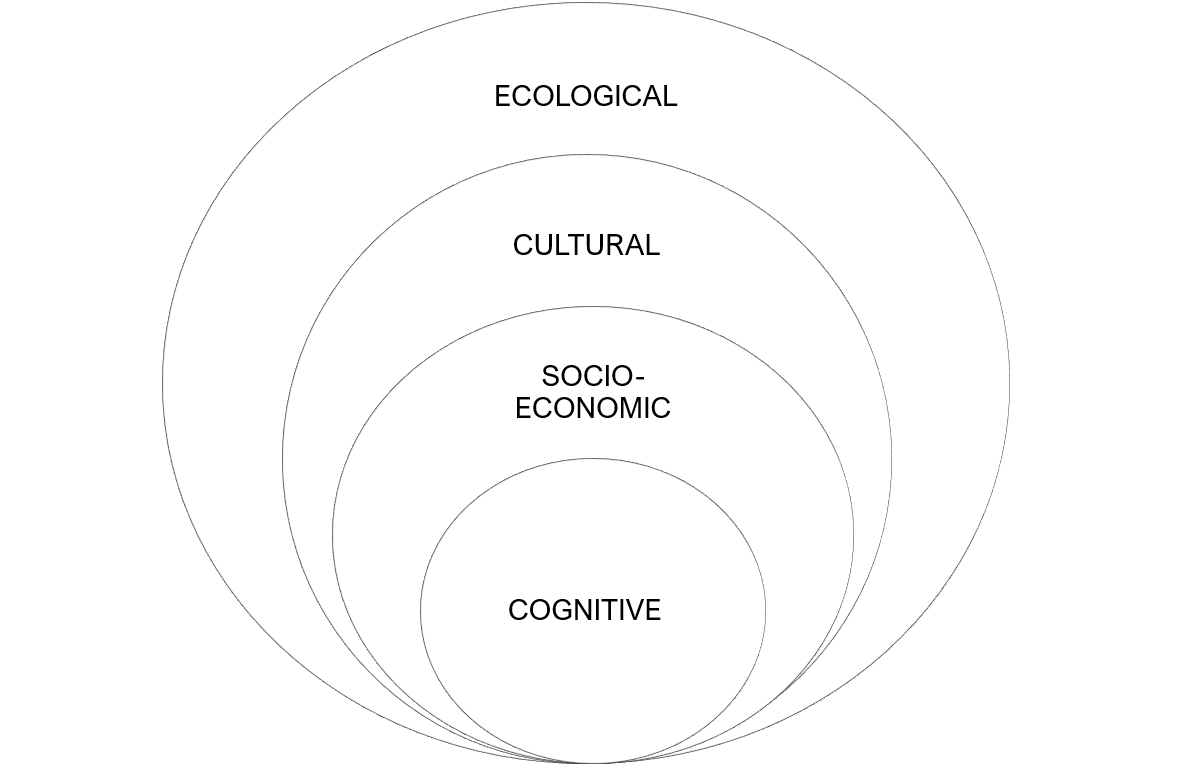
\includegraphics[width=8cm]{Figures/nested.png}
\caption{Levels of discourse analysis proceeding from the ecological macro-context of natural systems, to the micro-context of cognition}
\label{fig:figure1}
\end{figure} 

Discourse analysis is employed to gain insights into communication within and between the levels. These insights might include rhetorical styles, linguistic devices, power relations, ideologies, biases, identities, and other phenomena that may not be apparent on the surface of communication. Discourse analysis is concerned with naturally occurring language beyond standard linguistic units of analysis (i.e. morphology, semantics, and syntax). The `larger' units of interest to discourse analysis include texts, conversations, speech acts, or other communication events. The term discourse can apply to a broad range of communication. It primarily refers to language-in-use \citep{Wetherell2001}, but might also extend to nonlinguistic or multimodal communication including gestures, film, media, art, and sound \citep[2, 15]{Wodak2009}. 

In the sections that follow, each of the levels is outlined, with examples. Discourse is categorized under a given level primarily based on the semantic content. However, the extra-linguistic context is also important. Each level has two main elements: (i) the \textit{data} which refers to the communication itself; and (ii) \textit{analysis} of that data. 

\subsection{Ecological Level}

In the simplest terms, the ecological level refers to discourse about the natural world or the environment [\textit{Umwelt}]. This could obviously cover a wide range of communication, encompassing scientific statements or, outside of formal science, statements about the more-than-human world. The ecological level follows from the formal definition of ecology as a ``branch of biology dealing with the relations and interactions between organisms and their environment.''\footnote{https://www.dictionary.com/browse/ecology} In addition, the ecological level is concerned with human subjective experiences of the natural world and their surroundings. For instance, the present use of the term ecology also accounts for Jakob von Uexk\"ull's (\citeyear{VonUexkull1982}) semiotic concept of \textit{Umwelt}, which refers to the environment as the organism's centre of communication and signification rather than biophysical flows of material and energy (as in the strictly natural scientific concept of the environment). In other words, the \textit{Umwelt}, as experienced by the human subject, is the source of signification and meaning not only for the individual subject, but that is shared (intersubjectivity).

To illustrate what communication would be considered ``ecological,'' consider both of the following statements:

\begin{footnotesize}
\begin{itemize}
    \item[-] \texttt{Biodiversity has declined 27 percent in the last three decades.}
    \item[-] \texttt{I love to walk in the forest.}
\end{itemize}
\end{footnotesize}

The first statement is an empirical assertion that falls within the formal study of ecology. The second relates to a subjective experience of the natural world. In the present discourse analytic framework, both statements would be considered as part of the ecological level. The analysis of the statements would depend on the context. For example, if the above statements were placed in the following contexts, their interpretation would change considerably:

\begin{footnotesize}
\begin{itemize}
    \item[-] \texttt{Biodiversity has declined 27 percent in the last three decades, which justifies the total overhaul of our political and economic system.}
    \item[-] \texttt{I love to walk in the forest...experiencing nature is part of my identity and values as someone from rural Vermont.}
\end{itemize}
\end{footnotesize}

These contexts demonstrate how the levels are not distinct; rather, they often blend together. As discussed in later sections, the first statement would be analyzed with the socio-economic level while the second would be considered cultural.  

The ecological level obviously relates to natural sciences and scientific communication. It should be stressed, however, that the present study does not aim to employ methods of the natural sciences and, accordingly, the ecological level of analysis is not intended as scientific analysis. In line with critical science studies, scientific discourse is viewed in a social and cultural context, as having a semiotic role. Thus, the ecological level of analysis aims to bridge the social/human and natural sciences while maintaining critical, meaning-centred analysis. Such an aim is consistent with that found in political ecology literature. \cite*{Escobar1999}, for instance, refers to ``a new articulation of the natural and human sciences'' where the ecological realm is ``understood in biological terms but [also] in complex relation with cultural and economic practices'' (15). Along the same lines, \cite*{Peet2011} see natural sciences as ``essential to solving environmental problems'' but also as ``historically problematic parts of those problems'' (31). The aim is to employ a critical humanistic framework that challenges the so-called objective position of the natural sciences, but also accepts the crucial role for the scientific method in understanding and addressing ecological issues. 

To summarize, the ecological level \textit{data} consists of communication about the environment which often includes, but is not limited to, scientific communication. Ecological-level \textit{analysis} of that data is concerned with the social, cultural, and semiotic dimensions of ecological communication.

\subsection{Cultural Level}

A challenge for intercultural communication research is the very meaning of `culture'. In 1871, the anthropologist Edward Tylor offered a broad definition of culture as ``that complex whole which includes knowledge, belief, art, law, morals, custom, and any other capabilities and habits acquired by man as a member of society'' \citep[1]{Tylor1871a}. Ever since, scholars have been attempting to add specificity to Tylor's definition, focusing on external artefacts and behaviour; symbolic meanings; or psychological dimensions \citep[see][for an overview]{Prinz2016b}. To this day, there is a ``lack of clarity and consensus'' concerning culture \citep[12]{Minkov2013a}. The widespread use of the term, together with its ambiguity, has led some to dismiss scientific use of the concept altogether \citep[e.g.,][]{Barber2008a}. 

\cite*{Blommaert2005a} asserts that it does not make sense to speak of ``noncultural'' discourse (4). This statement reflects the notion that culture is ubiquitous \citep[15]{Neuliep2018a} or ``everywhere'' \citep{Hannerz1993a}. Given this sweeping scope, the question for a multilevel approach is how to distinguish culture from other levels. Since a potential drawback of multilevel research is its broad scope \citep{KleinK.J.TosiH.&Cannella1999a}, it is particularly important to avoid compounding this drawback through an overly broad view of the term culture. An overly broad view could, for example, lead one to characterize misunderstandings as intercultural when economic, political, or other social factors would provide a more accurate and descriptive account. In the opening chapter, for example, the failure of global climate change policy is discussed as one such example where political and economic factors are more likely at play than cultural differences. In order to analyze such complex issues, we can aim to delimit culture from other levels of social interaction.

To study how culture is reflected in discourse, various frameworks have been proposed including ``cultural discourse analysis'' \citep{Carbaugh2007a} and ``cultural approaches to discourse'' \citep{Shi-xu2005a}. Cultural discourse analysis (CuDA) draws out the ``symbolic meanings'' and ``cultural commentary'' that pervade human communication \citep[168]{Carbaugh2007a}. Other methods related to the cultural aspects of communication include ethnography of communication \citep{Hymes1972a} and speech codes theory \citep{Philipsen1997a}.

For the present multilevel framework, the cultural level refers to when people are expressing or commenting on who they are. Cultural discourse generally reflects one's identity, values, or worldviews. For instance, the following are some examples of statements that would fall into the cultural level of analysis.

\begin{footnotesize}
\begin{itemize}
    \item[-] \texttt{This is my home, and I will protect it.}
    \item[-] \texttt{God will take care of us.}
    \item[-] \texttt{Our ancestors would be proud.}
    \item[-] \texttt{I am American but France is my real home.}
\end{itemize}
\end{footnotesize}

Whether a statement is cultural will often depend on who the speaker is and how they identify as a member of a group. For instance, if speakers refer to themselves with a cultural or ethnolinguistic identity, then it is more likely that their words are expressing something with cultural significance. For instance, the following quote shows cultural self-identification.

\begin{footnotesize}
\begin{itemize}
    \item[-] \texttt{As indigenous women, we are here to protect our community.}
\end{itemize}
\end{footnotesize}

The above example contrasts with cases where an identity is assigned to another in the discourse, such as in the following statement:

\begin{footnotesize}
\begin{itemize}
    \item[-] \texttt{The protestors, who were mostly migrants from Mexico, were unruly.}
\end{itemize}
\end{footnotesize}

Here, the national/cultural identity \textit{Mexican} is assigned by the narrator. Such cases might still be considered cultural-level discourse, but likely with more critical analysis of the assigned identity. For instance, the cognitive dimension of stereotype might come into play in the analysis of this statement.

To summarize the cultural level, \textit{data} consists of communication that expresses meaning or identity in some way. The nonverbal component of the cultural level is also important, as speech style, gesture, and dress are all important elements of culture. \textit{Analysis} at this level asks how culture is being expressed, or what worldviews are implicit in the communication. At the cultural level we are cognizant of how identities are assigned. Being wary of stereotype and othering is crucial in this level of analysis.

\subsection{Socio-Economic Level}

The socio-economic level relates to what has typically been the focus of Critical Discourse Analysis (CDA). CDA is generally concerned with how social power relations are established and reinforced through language \citep{Fairclough1995}. Central to CDA are explicit or implicit goals of social change, which presuppose certain shared notions of justice, equality and `the good'. Critical analysis aims to expose and resist oppressive economic, social, and political structures that are enacted and perpetuated through language and communication. Beginning with the critical turn in the 1990s, CDA influenced critical intercultural communication \citep{Moon2011a}. 

The current multilevel framework\textemdash while maintaining an emphasis on critical analysis\textemdash distinguishes between the cultural and social realms. The social-level encompasses statements about economics, institutions, laws, and power relations. The following are examples of statements that would fall into the social level:     

\begin{footnotesize}
\begin{itemize}
    \item[-] \texttt{Unemployment in the community is higher than the national average.}
    \item[-] \texttt{Government and policy makers are only there to protect corporations.}
    \item[-] \texttt{The police used excessive force.}
\end{itemize}
\end{footnotesize}



\subsection{Cognitive Level} 

While many discourse analytic approaches study the relations between society, culture, and discourse, a socio-cognitive approach considers these relations as mediated by cognition \citep[64]{VanDijk2015a}. Attitudes, ideologies, and beliefs stem from cognitive structures that constitute social and cultural relations through discourse. Analogously, discourse establishes and reinforces cognitive structures. This link opens possibilities for intercultural communication research that is engaged with cognitive science while, at the same time, maintaining a social-critical edge. Here, we define the cognitive level of discourse as communication that provides insight into mental processes, particularly the unconscious. Cognitive level \textit{data} is any communication that provides these insights, while the \textit{analysis} seeks to arrive at the insights themselves. In other words, cognitive analysis establishes the relation between communication and mental representations. 

The cognitive level draws on concepts from cognitive linguistics. These concepts, which are developed in more detail in subsequent chapters, include the following:

\begin{itemize}
    \item \textit{Conceptual metaphor}: the understanding of one idea, or conceptual domain, in terms of another; a mapping between conceptual frames \citep{Lakoff1980a}. 
    \item \textit{Implicature}: inferential and context dependent knowledge domains or mental schema \citep{Grice1975}.
    \item \textit{Conceptual Blending}: how the combining and mapping of concepts gives rise to meaning as an emergent structure beyond the sum of its parts \citep[403]{Evans2006a}
    \item \textit{Idealized Cognitive Models}: the background knowledge that structures our mental spaces \citep{Lakoff1987}.
    \item \textit{Stereotype and othering}: categorizations that help to simplify and organize information, often manifesting as in-group/out-group generalizations \citep{Tajfel1981}.
    \item \textit{Nonverbals \& Emotions}: gestures, facial expressions, paralanguage and other nonverbals as a reflection of unconscious cognitive processes. 
\end{itemize}

Cognitive analysis plays an important role in understanding and interpreting communication beyond explicit written or spoken words. The other three levels of analysis rely more on explicit semantic content of utterances. The cognitive level, by contrast, relies more on implicit context, linguistic devices, and nonverbal expressions.

Cognitive level \textit{data} would be excerpts or examples of communication that demonstrate cognitive concepts, such as metaphor, implicature, blending, etc. Data also consist of visual and multimodal communication that permit the analysis of nonverbal communication. \textit{Analysis} relates to the interpretation of the data as well as insights concerning how cognition may be the basis of communicative misunderstandings.   

\subsection{Summary of Levels}

The four levels are summarized in Table 2.1 below. To separate levels in this way is, of course, a simplification. In reality, these factors blend together and there are not clear dividing lines between them. Ecological discourse is often cultural, the cultural and social realms are overlapping, and so on. Likewise, insights from cognitive linguistics do not apply to a subset of communication, they are features of communication itself. Nonetheless, in segmenting communication in this way, we are interested in prototypical examples of each level. Accordingly, we can better analyze each level and, ultimately, understand how the various levels interact.

\begin{table}[H]
\begin{footnotesize}
\centering
\def\arraystretch{1.5}% 
\begin{tabular}{ | P{4cm}| P{5.75cm} | }  
 \hline
\textbf{Level} & \textbf{Description} \\
 \hline
\textbf{Ecological} & Discourse about nature and the more-than-human world; includes discourse that concerns ecology in a scientific sense, as well as human subjective experiences (\textit{Umwelten}) \\
 \hline
\textbf{Cultural} & Expressions of identity, values, and worldviews; people commenting about who they are, either directly or indirectly  \\
 \hline
\textbf{Socio-Economic} &  Discourse related to economics, institutions, and power relations; aspects of social existence that do not express cultural identity \\
 \hline
\textbf{Cognitive} & Mental representations and cognitive frames as reflected in communication; drawing on concepts from cognitive linguistics as well as nonverbal communication \\
 \hline
\end{tabular}
\caption{Summary of levels of discourse}
\label{tab:table1}
\end{footnotesize}
\end{table}

\subsection{Levels of Communication Data}

Thus far, we've discussed levels as themes (ecological, cultural, socio-economic, and cognitive) to group the data and analysis. In addition to these four thematic levels, there are also multiple linguistic/communication levels, which relate to the type of data that is gathered. For example, in discourse analysis, one would consider different modes of communication such as texts, speech, body language, etc. Although discourse analysis has traditionally focused on the textual level, the term \textit{discourse} can encompass diverse forms and modalities of human communication.

For this study, communication data is segmented into three levels as outlined in Figure 2.2: (i) the textual level of written communication; (ii) the verbal level of spoken (lexical) communication; and (iii) the nonverbal level of spoken (non-lexical) communication. Like the thematic levels, these levels of communication are hierarchically ordered from general to specific, or from the macro- to micro-context. Multimodal communication is the blending of the three levels and is more representative of communication in real life.

\begin{figure}[H]
\centering
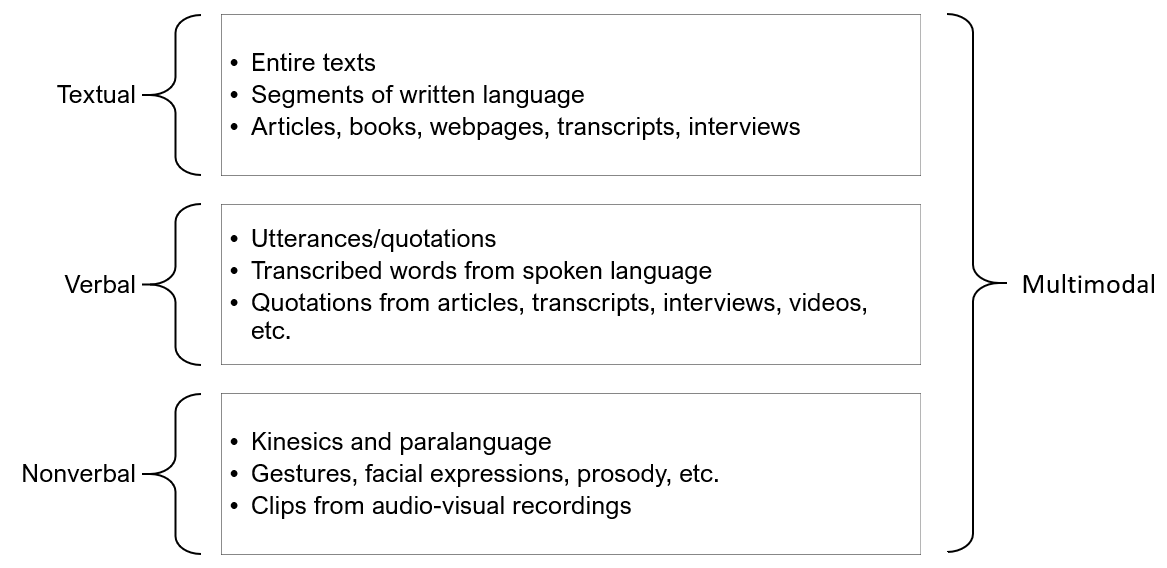
\includegraphics[width=12cm]{Figures/levelscomm.png}
\caption{Levels of communication with examples of data}
\label{fig:figure1}
\end{figure}

The \textbf{textual level} is concerned with entire texts and segments of language beyond utterances and sentences. Objects of textual analysis include articles, book excerpts, webpages, transcripts, and interviews. Of interest at this first level are broad themes, keywords, and rhetorical styles. The \textbf{verbal level} concerns utterances or statements made my a specific individual or possibly a group (e.g. group chants, slogans, etc.). In addition to their original source, utterances are obtainable from quotations in articles, transcripts, videos, or interview segments. As with the textual level, themes, keywords, and style are all of interest and serve as context for analysis. However, what distinguishes the verbal from the textual level is the identity of the speaker. Whereas textual data abstracts the speaker away from the text, the verbal level links utterances to a specific speaker. Finally, the \textbf{nonverbal level} considers nonlinguistic communication which may be visual, auditory, tactile, or kinesthetic. Gestures, facial expressions, pitch, and intonation are all examples of nonlexical components that are essential to meaning.

Of course, as with the thematic levels, textual, verbal, and nonverbal communication are not entirely separable in the flow of everyday life. Meaning and understanding arise from the interactions of these elements into multimodal, semiotic events. However, organizing data and analysis in a way that isolates the various elements allows for the investigation of the otherwise overly complex phenomena of human communication.

\section{Corpus Linguistics}

Above, we introduced four levels of analysis related to themes of discourse as well as three levels of communication data. This section addresses the data collection itself; that is, how we obtain representative samples of data that cover the levels and from which meaningful insights can be drawn.

When it comes to data collection, some trade-offs have to be made. As alluded to above, the very notion of communication as ``data'' is a simplification in that holistic semiotic events in the \textit{Lebenswelt} are categorized and isolated in order to be studied. Yet, to study a phenomena in a systematic way, we often need to move away from holistic communicative events and towards analyzable components. To decontextualize and reduce communication in this way simplifies complex phenomena. What's gained from this simplification, however, is generality and the ability to draw insights from a broad range of communicative situations. By employing different modes of inquiry (both qualitative and quantitative) the present methodology aims to strike a balance in a way that leads to generalizable conclusions while appreciating the complexities and nuances of communication and culture. 

This section introduces corpus-based approaches to both ecological and intercultural communication. Based on the lack of existing corpora in these areas, the case for custom, specialized corpora is made. Corpora constructed specifically for the present research problem are then discussed, in addition to how they are analyzed in subsequent chapters.

\subsection{The Need for Data Volume \& Variety}

To gain meaningful insights, data must be collected and patterns observed across a variety of situations and settings. In other words, a large volume and variety of communication needs to be analyzed. A multilevel approach only adds to these data requirements. To carry out ecological, cultural, social, and cognitive analyses requires data covering a wide range of themes and subject matter. Likewise, we need a combination of textual, verbal, and nonverbal data. A key methodological criterion, therefore, is the ability to gather and analyze a sufficient variety and volume of real human communication.

For the research question at hand, many common methods of intercultural communication research would be insufficient in terms of meeting the data requirements. These methods include ethnography of communication, interpretive interviews, postcolonial ethnography, and critical discourse analysis \citep{Oetzel2016a}. Ethnography of communication often requires extensive field work, which limits the geographic and temporal scope. Face-to-face interpretive interviews have similar scope limitations. While these and similar methods (involving primary-source data collection) are essential for a first-hand understanding of cultural and communicative events, they often limit the amount of data that can be collected. By drawing from secondary sources, CDA and other discourse analytic approaches allow for more data volume, but are still limited by the amount of linguistic data the researcher can read and interpret. Discourse-based methods often emphasize qualitative analysis through close reading of texts as well as interpretation of the extra-linguistic context. With this emphasis comes obvious limits to the amount of text a researcher can qualitatively assess. 

\subsection{Corpus Linguistics to Address the Data Challenge}

Ideally, a methodology would combine the emic depth of ethnographic field studies with the breadth and generality possible with large and varied data sets. However, these two aims are often inversely related. To strike a methodological balance, the present study proposes corpus linguistic methods for data collection and analysis. Corpus linguistics is one way to meet requirement for large data sets. In linguistics, a corpus is a collection of machine-readable texts stored in an electronic database \citep[48]{Baker2006c}. While a corpus does not contain new information, computer aided analysis can offer ``a new perspective on the familiar'' or insights that would be impossible through human analysis alone \citep[2-3]{Hunston2002a}. As \cite*{Belcher2013a} point out, digital corpora allow for a ``breadth or sheer numbers of texts and depth of analysis'' beyond what an individual could achieve ``despite their linguistic expertise and emic/etic cultural perspectives'' (1).

Several previous studies have effectively used corpora for discourse analysis. Large bodies of text allow for objective, quantitative approaches, adding to the generality and confidence of findings \citep[e.g.,][297]{Gabrielatos2008a}. These advantages are particularly pertinent given that a common criticism against CDA is that researchers can ``cherry-pick'' data samples based on their aims and assumptions \citep{Mautner2009a}. Although corpus approaches to discourse analysis have increased in recent years, applying corpus linguistics to either environmental or intercultural communication is even more recent and there are still relatively few corpus-based studies in these fields. 	

The methodological aim in this dissertation is to use corpus methods to study intercultural environmental communication. This aim leads to several questions pertaining to the size, balance, and representativeness of corpora which could be used for this purpose. A key question is whether existing corpora might be suitable or if new ones are required. Before addressing these questions, however, some more background is required regarding corpus linguistic approaches to both ecological and ICC research.

\subsection{Corpus Linguistics \& Ecology}

To consider how corpus linguistics might be applied to ecological questions we can look to the nascent field of ecolinguistics. Ecolinguistics is often traced to Haugen's (\citeyear{Haugen1972a}) introduction of the ``ecology of language'' as ``the study of interactions between any given language and its environment'' (325). Ecolinguistics became more prominent in the 1990s and was explicitly linked with modern environmentalism by \cite*{Halliday2001a}, who drew connections between ``linguistic anthropocentrism'' and unsustainable growth. As a relatively new, evolving approach to both linguistic and ecological research, the precise definition and scope of ecolinguistics remains open to interpretation. Some emphasize a metaphorical understanding of language as a living system, while others are more concerned with discourses that lead to environmental degradation \citep[see][for an overview]{Chen2016a}. An ecological approach to language raises a number of conceptual questions such as what constitutes the ecological context of language, or whether the relation between language and the physical environment is bidirectional or unidirectional \citep{DoCouto2014a}. Notwithstanding these challenges, ecolinguistics has emerged as an important interdisciplinary approach to both environmental and linguistic research. 

Although corpus methods have been effectively applied to ecolinguistic questions \citep[e.g.,][]{Poole2016a, Poole2018, Stibbe2003a}, there are many unexplored research questions suited to corpus approaches. Many of these questions carry over from existing areas of linguistic inquiry \citep[see][]{Cheng2012a}. For example, questions might concern new uses and meanings of words. As with other regions of language, words related to nature, landscapes, or species are continuously evolving. Consider the term ``wetland'' which was adopted to euphemistically replace ``swamp'' and came into scientific use in the latter half of the twentieth century \citep{NationalResearchCouncil1995}. Corpus approaches could provide insight into the evolution of such terms, including the historical and cultural factors surrounding use changes. In addition, even though the term has important legal implications, there is ambiguity regarding what exactly constitutes a wetland. There is, therefore, a role for corpus research in understanding the diverse uses of ecological terms by different groups.

Ecolinguistic research also investigates how grammar or lexical semantics construe the natural world in certain ways or possess anthropocentric properties. The passive voice, for instance, might be used to avoid human agency and responsibility \citep{Kahn2001a}. The use of pronouns (e.g. relative, personal, and possessive) in reference to nonhuman animals might also provide insight into human attitudes and behaviors towards other species \citep{Gilquin2006a}. The contextual meaning of lexical items will also frame and reflect the human relation to other species. \cite{Stibbe2003a}, for instance, refers to the British National Corpus (BNC) to demonstrate how pigs have overwhelmingly negative connotations compared with other animals. Grammar and semantics may also reveal taken for granted worldviews or ideologies that have profound environmental consequences. \cite*{Halliday2001a} points out how use patterns of forms of the word ``grow'' (e.g. growth, growing) reveal how ``deeply emgrammatized'' growth is in modern language and culture. The cross-linguistic study of lexical semantics could also provide insight into different meanings and cultural linguistic constructions of the natural world. For example, it has been argued that pronoun drop in certain languages (e.g. Japanese) may moderate individualism and perhaps even affect the environment-culture relationship \citep{Kashima2003a}. 

Ecolinguistic questions can also be investigated through inquiries into genre analysis, professional communication, or media discourse. For instance, assembling a specialized corpus of Environmental Impact Assessments (EIA) or other regulatory processes would enable comprehensive analysis of this genre of communication which is the standard in development and land use change. Along these lines, \cite{Sousa2012} applied corpus methods to regional planning rhetoric, concluding that there was a discourse orientation towards development rather than conservation. As environmental issues have become global and mainstream, critical approaches might analyze stereotyping and bias in environmental discourses \citep{Muhlhausler2006b}. Analysis of political or corporate discourses might also address the framing of environmental issues, power relations, and other themes related to political ecology and environmental justice. In all cases, corpus methods allow for comprehensive analysis of otherwise unsurveyable volumes of linguistic data.

The above examples concern the impacts of language on the environment. In other words, the research questions are based on a notion of ecolinguistics as discourses or clusters of linguistic features that impact the human relation to the ``natural world'' \citep{Stibbe2014b, Alexander2014a}. However, one could also understand ecolinguistics as involving the reverse relation, whereby the external environment is ``participating in language'' \citep{Cowley2014a}. This reciprocal relation between language and the natural world touches on a more contested aspect of the ecolinguistic paradigm, since the very premise that language is interconnected with the external world runs counter to established theories of language, notably Saussurian structuralism and Chomskyan generativism. The notion of an ecological theory of language is described as:

\begin{quote}
...a linguistic and trans-disciplinary approach that generates empirical hypotheses which describe and explain the manifestation and organization of linguistic processes in organism-environment relations \citep{Bang2014}. 
\end{quote}

Compared with research based on the previous definition of ecolinguistics (i.e. discourses that impact the natural world), corpus research working from an ecological theory of language (i.e. language as a natural phenomenon) is perhaps more exploratory, challenging, or in need of data/methods which are not yet developed. Nonetheless, some precursors have begun to take shape through evolutionary dynamics of natural languages \citep[e.g.,][]{Liberman2007a}, sound symbolism \citep{Nuckolls1999a}, modelling drivers of the loss of language diversity \citep{Amano2014c}. Such research, supported by growing corpus data, might point to the notion of language or languaging as a biological phenomenon  \citep{Kravchenko2016b}; a complex, interconnected system that is best understood in ecological terms as a holistic semiotic environment or the ``deep experience of organic existence'' \citep{Firth1957a}. An ecological theory of language might similarly develop from the idea of languages and cultures as \textit{organic forms} (discussed in more detail in Chapter 6).

The wide range of interpretations of ecolinguistics leads to a range of possible methodological approaches to corpus research. One could draw on corpora to apply quantitative/statistical methods to test hypotheses. By contrast, corpora could be used alongside ecopoetics or other humanistic modes of inquiry that account for meaning, symbolism, and phenomenological experience. This present study touches on ecologinguistics in a number of ways including examining how scientific language is employed in the public sphere; cultural meanings associated with the natural world; and, how ecological themes overlap with other layers of discourse. 

\subsection{Corpus Linguistics \& Intercultural Communication}

One challenge for corpus-based intercultural communication research is that textual data alone is insufficient for analysis of microcultural and metalinguistic interactions. Corpora decontextualize language. By reducing communication to text (neglecting body language, intonation, gesture, etc.) linguistic corpora are often ``semiotically impoverished'' \citep[34]{Mautner2009a}. This limitation is a possible reason why corpus-based methods have not fully taken hold in intercultural communication research as compared to emic methods like ethnographic field studies or interviews.	

It is possible, however, to use corpus methods to study a wider range of communication than written text. Despite the text-focus of many corpus studies, there are examples of corpora that contain aural/visual, nonverbal, and paralinguistic elements. The \textit{Hong Kong Corpus of Spoken English} \citep{Cheng2005a} is one case of a corpus with voice recordings that has been used for intercultural communication research. This corpus is comprised of 106 hours of spoken discourses and has been used in studies related to discourse intonation and intercultural understanding \citep[e.g.,][]{Cheng2007a}. The VOICE Corpus (Vienna-Oxford International Corpus of English) and the ELFA Corpus (English as a Lingua Franca in Academic Settings) also consist of recordings of intercultural encounters, specifically among those whose first language is not English  \citep[118]{Lee2010a}. These examples suggest that the study of multimodal and holistic communication is compatible with corpus approaches.

There are also several examples showing that text corpora can indeed address intercultural communication research questions. Many of these examples derive corpus data from published books and media. For instance, \cite*{Almujaiwel2018a} analyzes and quantifies instances of ``interculture'' in ESL texts by identifying cultural topics (``nodes''). \cite*{Popescu2013a} have students analyze similarities and differences in collocations between English and Romanian using a corpus of business press articles. Other studies draw from publicly accessible websites. \cite{Hua2017a} examine how intercultural communication is framed in online higher education promotional discourse. Similarly, \cite{Ming2015a} use corpus assisted analysis of websites to look at corporate identity construction in China and the US. Still others leverage the data of Web 2.0 by building ``intercultural'' corpora from social networking sites, wikis, and online forums. \cite*{Orsini-Jones2016a} look at pronoun use in a corpus from an intercultural online exchange. \cite*{Ryshina-Pankova2018a} take a similar approach to examine intercultural discourse in telecollaboration between German and US students. Finally, \cite*{Fina2011a} uses a corpus of TripAdvisor reviews to do an intercultural analysis of travel preferences.

Among the various intercultural studies using text corpora, a commonality is that researchers constructed a corpus specifically for the question at hand. In other words, publicly available `off the self' corpora were not used. One possible explanation is that corpora are often built to reflect a specific linguistic or national community rather than being explicitly intercultural or multilingual. However, this is only a partial explanation since there are parallel, comparable, and multilingual corpora that allow for cross-cultural analysis. A more likely explanation is simply that linguistic data is readily available and a custom corpus is the most effective way to address a specific research question. 

\subsection{Three Multilevel Corpora \& Analyses}

The research question for this dissertation is pursued using custom-built corpora as opposed to using existing corpora. The rational for this methodological decision is the limitations of general corpora for the subject of environment and ecology. In addition, intercultural communication demands consideration of all levels of communication. Simply put, there are no existing corpora that combine ecological subject matter with multiple modes of communication.  

Previous studies show corpus analysis can be a useful tool for ecolinguistic research, but the limitations encountered (i.e. low frequency words and necessity of manual data cleaning) point to the need for corpora and annotation schemes specific to ecolinguistics. \cite{Frayne2019} found that, despite using two of the largest available English language corpora, it was difficult to obtain data in sufficient volume and variety for targeted ecolinguistic research. A corpus consisting of texts covering a variety ecological themes, would help ensure higher frequency of ecological vocabulary and allow for more in-depth, specialized research. Also, a corpus with searchable content from different regions would allow for comparative analysis of environmental discourses based on culture, geography, or historical factors. A corpus of more breath and depth of ecological content would allow questions in previous corpus approaches to be investigated at larger spatial-temporal scales.

Examining the status quo of corpus-based intercultural communication leads to similar conclusions. Publicly available data sets may be good starting points, but more `tailor made' corpora are often necessary to pursue in-depth research questions. Moreover, with the deluge of global digital communication, the largest and most accessible corpus for intercultural communication may be the web itself. What follows is a description of web corpora built specifically for this research project. 

It is to sweeping a task to create a corpus which reflects all levels of communication. It is likewise overly ambitious to set out constructing a single corpus to be representative of all environmental discourse. For this reason, for the current research problem, three distinct corpora were constructed. Each corpus is aimed at a level of communication, so there is a textual, verbal, and a nonverbal corpus. Also, each corpus corresponds to an overall environmental theme. The themes covered are genetically modified (GM) seed, the Dakota Access Pipeline (a natural gas infrastructure project), and mining.

The specific methodologies for constructing each of the three corpora are outlined in chapters 3, 4, and 5, respectively. They are summarized in Table 2.2 below. 

\begin{table}[h]
\begin{footnotesize}
\centering
\def\arraystretch{1.5}% 
\begin{tabular}{ | P{1.5cm} | P{3.5cm} | P{4cm}| }
\hline
\textbf{Corpus} & \textbf{Themes}  & \textbf{Data} \\
\hline  
1 &  \makecell[l]{Genetically modified \\ (GM) seed}                & Texts collected from the web; categorized into 2 sub-corpora representing pro- and anti- sides of the debate                      \\
\hline
2               & \makecell[l]{Dakota Access Pipeline \\(natural gas pipeline)} & Quotations, parsed from web articles, with speaker identities; categorized into 3 groups depending on the position of the speaker \\
\hline  
3   &\makecell[l]{Mining \& Resource \\ Extraction} & Video interviews and documentaries; transcripts recorded and nonverbal annotation applied to selected segments  \\ 
\hline  
\end{tabular}
\caption{Summary of the corpora used for multilevel analysis}
\label{tab:table1}
\end{footnotesize}
\end{table}

The aim is to conduct an analysis of each corpus (1 to 3) in a way that proceeds from the general to the specific, or from the macro to the micro levels of communication. Analysis 1 looks at broad themes from the perspective of the entire texts. Analyses 2 and 3 proceed to sentences, phrases, and even the phonetic and syllaballic components of linguistic data. The three levels of discourse are applied to each corpus. In other words, each the three analyses is split into ecological, cultural, socio-economic, and cognitive levels. 

\subsection{Analysis 1}

Analysis 1 corresponds to the highest level of communication in the sense that a general macro view of the corpus data is sought. The data consist of texts which include articles, web pages, transcripts, legal documents, and interviews. This level looks at speakers/producers of texts as an aggregate, rather than considering specific speakers or groups. This view includes dominant themes and lexical features observed across the entire corpus. To this end, Analysis 1 makes use of quantitative and computational techniques more than the other analyses. The specific methods used in Analysis 1 are summarized as follows:   

   \begin{itemize}
     \item \textit{Keyword Analysis} involves identifying words and phrases that appear in the corpus at a higher frequency than would be expected by chance \citep{Scott2006}. This allows for identification of key themes and motifs in the corpus.
     \item \textit{Concordance} or \textit{key word in context (KWIC)} is a list of all the particular search terms in a corpus as well as the context in which the terms occur \citep[42-43]{Baker2006c}. Concordances allow linguistic patterns to be discerned such as the meanings of words.
     \item \textit{Time Series} trends can reveal patterns of linguistic change across time. This generally involves plotting frequencies of words or entities.
     \item \textit{Type-Token Ratio (TTR)} is obtained by dividing the types (unique words) in a corpus by its tokens (the total number of words). A high TTR generally indicates a high degree of lexical variation.
     \item \textit{Collocation} is a sequence of words that co-occur more than could be expected by chance. Collocates can be indicative of semantic relationships and associations in the corpus.
   \end{itemize}

The corpus (Corpus 1) is split into two subcorpora, representing pro- and anti-GM perspectives. The aim of Analysis 1 is to gain understanding of the differences between the two perspectives. The premise is that by comparing the subcorpora through keyword analysis, concordances, collocations, etc., aspects of the data can be discerned that would not emerge if one were to simply read the texts manually. That said, obtaining a macro view of the data does not replace manual analysis; rather, it uncovers patterns for more detailed investigation and interpretation.     

Analysis 1 begins with the ecological level by asking how the natural world and ecological themes are construed in each subcorpus. A hypothesis of this analysis is that language used to express natural scientific and ecological concepts will entail different epistemological frameworks for understanding and relating to the natural world. Moreover, language used at subsequent levels of analysis (i.e. cultural, socio-economic, cognitive) sheds light on possible sources of epistemological differences. Of particular interest is how the cultural context influences the way people speak and think about GM-seed. So, after investigating the ecological level, the focus turns to cultural differences in the supcorpora. Whether there is regional or national variation in the data may be indicative of cultural difference. The historical context as well as references to people, places, and events is also be considered.

\subsection{Analysis 2}

Analysis 2 considers verbal data, corresponding to the meso-level of communication. Where the macro-level was interested in broad intertextual trends in the data, the meso-level takes a narrower view by looking at sentences and phrases spoken by particular individuals. Quotations of pipeline proponents are analyzed alongside those of pipeline opponents (both indigenous and non-indigenous). Moreover, in contrast to Analysis 1, the identities (professional, ethnic, social, etc.) of the speakers are taken into account. 

Whereas Analysis 1 begins with quantitative and computational methods, Analysis 2 relies more on qualitative and manual techniques. Analysis 2 begins with a similar question as Analysis 1; namely, how ecological topics are communicated among the different groups. The focus then turns to the cultural and socio-economic levels. This focus is achieved through both cultural and critical discourse analytic methods.

Cultural discourse analysis (CuDA) is adopted as a method that draws out the ``symbolic meanings'' and ``cultural commentary'' that pervade human communication \citep[168]{Carbaugh2007a}. CuDA seeks to identify the meanings, significance, and meta-cultural commentary active in the described communication \citep[172-74]{Carbaugh2007a}. Analysis 2 builds on the distinction (introduced earlier) between cultural and socio-economic levels. In contrast to the notion that cultural meanings are active in all communication, a hypothesis of Analysis 2 is that a subset of the quotations will pertain to the cultural realms of identity, values, ethnicity, etc. In other words, in the multilevel framework, only a certain subset of quotations from pipeline opponents qualify as cultural discourse. To put it another way, even if we accept that culture is imminent in all communication, a segment of the quotations contain layers of cultural meaning not inherent in the other quotations. By contrast, communication might be better described as institutional, corporate, or legal (i.e. the socio-economic level of analysis). 

A central aim of Analysis 2 is to explore the interrelations between the cultural and socio-economic levels. For instance, one question is the extent to which opposition to the pipeline stems from cultural differences or whether it is better explained in terms of economic inequalities. Another question concerns how cultural identity or group membership intersects with socio-economic status. ``Discriminatory discourse strategies'' \citep{Escamilla2013} such as ``otherization'' and stereotype are investigated at the cognitive level. 
     
\subsection{Analysis 3}

Analysis 3 deals with nonverbal, multimodal data. The nonverbal level looks at gestures, expressions, and paralanguage, which often take place within and between spoken words. Within the multilevel framework, Analysis 3 depends on cognitive level analysis. The premise is that communication consists of largely unconscious nonverbal elements (body language, facial expressions, eye movements, etc.) that are essential to meaning and interpretation \citep{Massaro1987}. Gestures, for instance, have been found to be essential not only to communication, but to thinking itself \citep{McNeill1992, McNeill2005b}. Accordingly, an aim of Analysis 3 is to interpret meaning beyond explicitly spoken words.     

Although the nonverbal analysis goes beyond what is verbally communicated, it does not neglect the verbal. To the contrary, nonverbal communication is seen as a way to enhance understanding of the textual and verbal expressions that it occurs with. The nonverbal expressions often complement what is being verbally communicated \citep{Kendon2004} or might even carry a more precise meaning than the words \citep[316]{Evans2001}. From the multimodal corpus, the aim is to identity moments where speech and nonverbal expressions combine to underscore a certain meaning. These moments are what \cite*{McNeill2005b} calls points of ``highest communicative dynamism'' (1).

\section{Summary}

This chapter began by stating the challenge of intercultural communication research and the need for interdisciplinary, multilevel approaches. Over several decades, the discipline of ICC has spanned microcultural and metalinguistic elements of communication as well as macrocontext of social and economic systems. The ecological turn can be considered a further movement towards the macrocontext. However, the true strength of ICC lies in combining this macrocontext with the microcontext of human communication and culture. Critical research engaged with the cognitive sciences is one path to this combination.

To begin this task, multilevel discourse analysis is proposed. By distinguishing communication according to levels (ecological, cultural, socio-economic, and cognition) we can gain insights as to the meaning of communication and sources of misunderstandings. Furthermore, integrating different levels of data (textual, verbal, nonverbal) can account for the complex phenomenon that is human communication.

A methodological challenge to multilevel analysis is the data requirements. Corpus linguistics offers the possibility to obtain large, representative data sets. Since there are limited publicly available corpora suitable for the present research question, custom corpora were built. The next three chapters introduce and analyze these corpora.   % Methods 

\chapter{Analysis 1: Textual Analysis of GM Seed Discourse}
\lhead{\textit{Analysis 1: Textual Analysis of GM Seed Discourse}}

\textit{\textbf{Chapter Summary}: In this chapter, multilevel analysis is applied to a web-based corpus to examine debates related to genetically modified (GM) seed. Keyword analysis, concordance lines, and collocation are used to explore whether sides in the debate are reflected in the semantic structure of the text. Implicature and conceptual blending point to differences at the cognitive level. Results highlight how misunderstandings can emerge from differing epistemologies, worldviews, and situated contexts.}
\newline

Since its emergence on world markets in the 1990s, genetically modified (GM) food has been a source of controversy and disagreement. The disagreements involve a range of actors including consumers, farmers, multinational companies, regulators, non-governmental organizations, and scientists. Here, we use multilevel analysis to gain an understanding of opposing views on the subject of GM seed. Using corpus-based data and analysis, we contrast perspectives on the issue in order to identify sources of divergence. 	

The GMO debate often focuses on whether or not GM food is safe for human consumption. On the surface, the debate strictly concerns scientific evidence. However, even at the scientific-level, there is much variation in how statements and evidence can be interpreted. For instance, people might respond differently to the claim that there is no evidence of adverse health impacts. Moreover, how people respond to this claim may be influenced by culture, since ``no evidence'' indicates a degree of unpredictability or uncertainty. It is well established that uncertainty avoidance is culturally variable \citep{McCornack2017}.

In addition to debates concerning the science, there are many other aspects to the topic of GM seed. Practices relating to the production and consumption of food go to the core of many cultures and value systems. In addition, production and consumption of food is the basis of economic livelihoods and well-being. Given the many scientific, cultural, and economic dimensions of the topic, it is appropriate to approach GM seed debates through multilevel analysis. 

\section{Corpus Data}

The first corpus contains textual data related to the theme of GM seed. The aim for corpus construction was comparative analysis of two sides of the debate surrounding GM seed (i.e. pro and anti). Thus, the corpus was split into two sub-corpora representing anti- and pro-GM seed perspectives,3 respectively. 

Two sub-corpora were constructed using text from web pages. Web pages were queried and identified manually using the Google search engine with search terms related to GM seed. Some search terms were generic so as to capture perspectives from both sides of the debate (i.e. ``gm seed'', ``gm seed AND seed saving'', ``gm seed debate''). Other search terms were targeted towards a specific side of the debate (i.e. ``gm seed resistance'', ``gm seed opposition'', ``gm seed advantages'', ``gm seed benefits''). Finally, another generic search was included to identify cultural dimensions (``gm seed AND culture'').

For each search, pages were qualitatively identified as representing either an anti- or pro- stance on GM seed. Pages that were ambiguous or were of a `pros and cons' nature were omitted from further consideration, though it was noted that the vast majority were easily identifiable as pro- or con-. For those pages which did take a clear stand on the topic, the associated urls were collected and listed as either anti- or pro-GM seed. About 100 urls for each category were collected in this way. Both categories included pages from ngos, foundations, news agencies, social media, and academic institutions. As might be expected, the pro-GM category included more pages from corporations while the anti- category included more ngos and advocacy groups. Genres included news articles, op eds, blogs, academic articles, reference material, interviews, transcripts, and reports. Another important genre was advocacy statements for organizations.

Once urls were collected, the text from the associated webpages was extracted with a custom script written in the Python language. All texts were agglomerated into one file, such that there were two files, one for the anti- and one pro- corpus.\footnote{The files \textit{anti\_gm.txt} and \textit{pro\_gm.txt} are available in the GitHub repository (link provided in Appendix 1).} Each of the files was then cleaned to remove html tags and other unnecessary syntax. The result was two data files, each a corpus of texts from about 100 sources. After some initial noise removal (removal of punctuation, digits, and special characters), the size of the anti-gmo subcorpus was about 225,000 words while the size of the pro- subcorpus was about 163,000 words. 

To facilitate computational analysis, further pre-processing was done on both data sets using the Natural Language Toolkit (NLTK) Python package. Normalization of the data was done through stemming, lemmatization, and removal of stop words. After this normalization, the size of the anti-gmo subcorpus was about 135,000 words while the size of the pro- subcorpus was about 101,000 words. 

In what follows, the corpus is analyzed in order to shed light on various levels of the GM debate. Linguistic data are compared and contrasted from the two sub-corpora, representing pro- and anti-GM perspectives. Through the data, we seek to determine whether there are quantitative differences between the sub-corpora and, if so, how these differences can be qualitatively explained. For this, corpus methods are combined with discourse analysis. Employing quantitative analysis of large data sets in this way allows for insights that would otherwise not be discernible though manual reading of texts.

\section{Overview of the Data}

An overview of the corpus data provides possible directions for further analysis. This overview is obtained in two ways: first, by considering differences in the sources or the data for the two sub-corpora; second, by comparing keywords and key terms between the two sub-corpora.    

\subsection{Top-level Domains}

Differences in sources of the data refers to where/who the data originate from. As explained above, corpus data was collected from webpages. Understanding more about these webpages will help us understand the corpus as a whole. For instance, if a majority of the pro-GM data originated from webpages based in a specific geographic region, then this would be an important point for further consideration. The same would be the case if the majority of pro-GM webpages were from corporate websites. 

For a quick view of the webpage origins, we consider top-level domains (tlds). These are the last part of the web address. For example, in the domain name \textit{www.domain.com}, the top-level domain is \textit{com}. Top-level domains provide clues as to the origins of the data. For instance, the generic tlds such as \textit{com}, \textit{org}, \textit{gov}, \textit{edu} indicate whether the data originated from commercial, organizational, governmental, or educational bodies, respectively. Also, country code tlds such as \textit{fr} (France) or \textit{uk} (United Kingdom), give insight into the country origins of the data.   

To investigate tlds for the corpus, a list was constructed of all domains used in the data collection. Using Python, urls were parsed to determine the distribution of tlds. The pro-GM corpus was constructed from 89 webpages. Of the urls for these pages, 39 (44 percent) had \textit{org} as the tld and 29 (33 percent) had \textit{com}. The remaining tlds (21 total) were \textit{net}, \textit{edu}, \textit{ca}, \textit{uk}, and a handful of other country codes. The pro-GM corpus consisted of 91 urls of which 50 (55 percent) had \textit{com} and 25 (27 percent) had \textit{org} as the tdls. The remainder (16) were \textit{net}, \textit{edu}, \textit{gov}, \textit{ca}, \textit{uk}, and other country codes.

The numbers indicate that the anti-GM data represent a higher percentage of non-governmental or non-corporate organizations (with \textit{org} tlds), while the pro-GM data represent comparatively more corporate organizations (with \textit{com} tlds). As we go deeper into textual analysis, these basic observations about tdls may be helpful in determining sources of different perspectives on the topic of GM seed. A more in-depth look at organizations/people behind the data will be investigated in the multilevel analysis sections. 

\subsection{Keyword Analysis}

A first comparative glance of the sub-corpora can be obtained through keyword lists. Keywords are words typical of a focus corpus vis-\`a-vis a reference corpus. Classifying the top words compared to a reference corpus reveals a range of contrasts and characteristics of the focus corpus \citep{Kilgarriff2012a}. In addition to keywords, key terms (multi-word noun phrases) can be identified. Using the corpus query tool Sketch Engine, keyword and key term lists were obtained for both sub-corpora. Top words and terms were identified according to a score given by: 

\[ \frac{f_\mathrm{focus}+n}{f_\mathrm{ref}+n} \]

Where \(f_\mathrm{focus}\) is the frequency (per million) in the focus corpus and \(f_\mathrm{ref}\) the frequency in the reference corpus and \(n\) is a smoothing parameter (default \(n=1\)) \citep{Kilgarriff2014a}. The reference corpus was Sketch Engine's web corpus \textit{enTenTen: Corpus of the English Web}.	 

Keyword and key term lists provide an overview of the corpora and indicate possible avenues for further analysis. Below, Table 3.1 shows the top 20 keywords and Table 3.2 shows the top 10 (bi-gram) key terms along with the scores and focus frequencies for both the anti- and pro-GMO sub-corpora. 

\begin{table}[H]
\begin{footnotesize}
\centering
\def\arraystretch{1.1}%
\begin{tabular}{llllll}
\hline
\multicolumn{3}{c}{\textbf{Anti-GMO}}    & \multicolumn{3}{c}{\textbf{Pro-GMO}}   \\
\hline
\textbf{Word}        & \textbf{Score}  & \textbf{Freq.} & \textbf{Word}        & \textbf{Score}   & \textbf{Freq.} \\
\hline
monsanto    & 816.94 & 619   & ht          & 1710.97 & 665   \\
gmos        & 791.46 & 353   & eiq         & 1394.56 & 291   \\
peoples     & 642.26 & 554   & herbicide   & 857.48  & 591   \\
maize       & 576.19 & 379   & gm          & 768.84  & 1926  \\
gmo         & 477.85 & 324   & maize       & 757.65  & 395   \\
soya        & 352.18 & 151   & tillage     & 688.04  & 202   \\
biocultural & 321.83 & 85    & soybean     & 683.11  & 613   \\
indigenous  & 304.84 & 1097  & insecticide & 512.21  & 312   \\
herbicide   & 301.44 & 262   & ha          & 484.71  & 1114  \\
gm          & 297.41 & 940   & glyphosate  & 468.27  & 138   \\
bt          & 292.49 & 146   & bt          & 442.13  & 175   \\
transgenic  & 285.48 & 119   & ir          & 430.18  & 335   \\
genetically & 281.36 & 415   & monsanto    & 416.52  & 250   \\
biocultural & 244.12 & 66    & biotech     & 414.95  & 234   \\
sovereignty & 207.72 & 55    & crops       & 407.03  & 103   \\
roundup     & 200.43 & 94    & canola      & 390.11  & 179   \\
glyphosate  & 194.02 & 72    & gmos        & 331.37  & 117  
\end{tabular}
\caption{Keywords from the sub-corpora (ranked by score).}
\label{tab:table1}
\end{footnotesize}
\end{table}

\begin{table}[H]
\begin{footnotesize}
\centering
\def\arraystretch{1.1}%
\begin{tabular}{llllll}
\hline
\multicolumn{3}{c}{\textbf{Anti-GMO}}    & \multicolumn{3}{c}{\textbf{Pro-GMO}}   \\
\hline
\textbf{Word}        & \textbf{Score}  & \textbf{Freq.} & \textbf{Word}        & \textbf{Score}   & \textbf{Freq.} \\
\hline
food sovereignty & 406.57 & 126   & farm income & 1107.66 & 251   \\
traditional food & 300.48 & 94    & crop impact & 949.56  & 197   \\
bt maize & 218.5  & 57 & farm level & 456.68  & 99    \\
traditional knowledge & 218.43 & 82 & soil carbon & 391.81  & 88    \\
oilseed rape & 196.6  & 61 & carbon sequestration & 376.53  & 102   \\
biocultural diversity & 167.53 & 49 & bt cotton & 359.88  & 77    \\
seed market & 129.7 & 34 & income gain & 342.87  & 71    \\
genetic diversity & 125.82 & 46 & income impact & 331.91  & 69    \\
genetic engineering & 121.19 & 51 & weed control & 324.33  & 85    \\
seed sovereignty & 110.33 & 29 & herbicide use & 317.93  & 68   
\end{tabular}
\caption{Key terms from the sub-corpora (ranked by score).}
\label{tab:table1}
\end{footnotesize}
\end{table}

There are several keyword differences between the two sub-corpora. The anti-GMO subcorpus contains a higher incidence of culturally significant words and terms, notably \textit{peoples}, \textit{biocultural}, \textit{indigenous}, \textit{sovereignty}, \textit{traditional food}, \textit{traditional knowledge}, and \textit{biocultural diversity}. What these items suggest is that the anti-GM discourse is embedded in a context of group identities, traditions, and intersubjective meanings. In addition to the scientific and technical terminology (e.g., \textit{transgenic}, \textit{glyphosate}, \textit{Bt}), the cultural and social aspects are present in a way that they are not in the pro-GM data. 

By contrast, the pro-GM subcorpus features more technical and specialized words and terms. There are higher frequencies of abbreviations like \textit{ht} (herbicide tolerant), \textit{eiq} (environmental impact quotient), and \textit{ir} (insect resistant). The use of abbreviations suggests more dense technical discourse. The key terms list also features several items related to income, indicating that economic gain and efficiency is a more prevalent theme in the pro-GM corpus. 

Similar conclusions can be drawn by looking at the top n-grams (sequences of \textit{n} words). These were determined by taking the top frequencies on an absolute basis (i.e. not using a reference corpus for comparison). After removing stop words, the 20 most frequent uni-grams, bi-grams, and tri-grams (1-, 2-, and 3-word sequences) were determined for each corpus.

As expected, there are several top keywords common to both sub-corpora such as \textit{gm} and \textit{genetically modified}. However, there are also notable differences. For instance, in the top-20 lists obtained from the anti-GM corpus, the following n-grams are present:

\begin{quote}
\textit{indigenous}, \textit{people}, \textit{traditional}, \textit{cultural}, \textit{community}, \textit{food sovereignty}, \textit{biocultural diversity}, \textit{traditional knowledge}, \textit{agro ecological system}, \textit{right indigenous people}, \textit{sovereignty}, \textit{critical dialogue}.   
\end{quote}

These n-grams are indicative of a certain cultural as well as socio-economic context rooted in identity, tradition, and food sovereignty. By contrast, the pro-GM corpus features more abbreviations as well as technical language related to agrochemicals and agribusiness. For example, the pro-GM corpus contains the following n-grams in the top-20 lists:

\begin{quote}
\textit{ht}, \textit{herbacide}, \textit{cotton}, \textit{cost}, \textit{yeild}, \textit{gm ht}, \textit{gm ir}, \textit{farm income}, \textit{ht soybean}, \textit{yeild}, \textit{cost saving}, \textit{biotech crop}, \textit{farm income gain}, \textit{kg carbon ha}, \textit{income impact using}. 
\end{quote}

A preliminary view of the corpus suggests multiple discursive themes are present in the corpus. In addition to ecological/scientific aspects, culture seems to be a major factor in the anti-GM corpus. Also, the presence of economic terms suggests that socio-economic factors are also central, with \textit{income} and related terms featured more in the pro-GM corpus. Also, the pro-GM corpus seems to contain more abbreviations and terminology related to agrochemicals/agribusiness. 

As with the preceding data on top-level domains, these are only precursory observations and further analysis is needed before drawing any conclusions. 

\section{Multilevel Analysis}

The initial overview of the data suggests possible avenues by which to understand the GM seed debate. In particular, the keyword analysis confirms that the topic of GM seed touches on a complex interplay of scientific, cultural, and economic dimensions. Moreover, the data suggest that these dimensions differ between the between pro- and anti- perspectives.

The sections that follow look at each level separately, expanding on themes that emerged in the overview of the data.

\subsection{Ecological Level}

Chapter 2 introduced the ecological-level of discourse. This level asks us to consider the ecological context of language and communication. Simply put, the premise is that the way in which humans speak and communicate about the natural world matters. Communication about nature reflects deeply held worldviews and beliefs. Communication also constitutes environmentally destructive actions. This section applies the ecological level in the context of GM seed discourse. The corpus provides discourse surrounding GM seeds, allowing us to ask how this discourse reflects certain worldviews, values, and beliefs.  

GM seeds are those whose DNA has been modified using genetic engineering methods. One might question how something as fundamental as the molecular building blocks of organisms and life, concerns the realm of worldviews and human values. Or, more precisely, one might ask how is it that gene sequences\textemdash which are empirically measured and scientifically understood\textemdash can lead to clashes of worldviews and values. One explanation for diverging perspectives is that there are different, culturally variable, ways of understanding complexity and unpredictability. In the face of this complexity, views on whether and how humans interact with nature's processes (e.g., by altering plant DNA), might be culturally variable.

Ecology\textemdash as the study of how organisms relate to one another and their physical surroundings\textemdash aims to understand interactions from the molecular level all the way to entire organisms, ecosystems, and the planet itself. Ecological interactions give rise to emergent and interdependent complex systems \citep{Bar-Yam2002a}. While the scientific method provides insights into ecological interactions, the complex nature of these interactions may preclude surveyable, reductionist understandings. This unsurveyable characteristic of living systems might manifest as unpredictability. Gene editing and its ecological implications may fall into the realm of what \cite*{Jasanoff2003a} calls ``the unknown, the uncertain, the ambiguous, and the uncontrollable'' (227). 

Ecological complexity might also imply that, in addition to scientific understanding, humans interpret the natural environment semiotically. Chapter 2 posits that humans experience nature as semiosis; that is, nature itself is the source of signs and symbols to which humans ascribe meaning. Rather than third person spectators with an objective, subject-object relationship to nature, humans are embedded in nature and experience it first-hand. Thus, from a standpoint of humanistic inquiry, biological and ecological phenomena can be understood and interpreted metaphorically and symbolically. In other words, natural semiosis carries over into human (cultural) semiosis. Taking gene expression as a type of natural semiosis, discourse in the corpus might reflect how language ascribes meaning to nature, even at its most basic level of DNA. 

To summarize, the human understanding of nature is commonly thought of through universal laws obtained through the scientific method. However, nature is also culturally framed by worldviews (\textit{Weltanschaung}) \citep[217-228]{Dahl2016}. How people understand and communicate about of gene editing technology will depend on worldviews with which they make sense of biological and ecological systems. These worldviews may be heavily influenced by natural science, but also concern complexity, unpredictability, and even the unknown. Of interest in the ecological-level of analysis is whether and how the different sub-corpora reflect different worldviews or ways of understanding nature. 

\textbf{Specialization \& Communities of Practice}

Different understandings of nature can first be approached by looking at how specialized terminology is used in the corpus. Tables 3.1 and 3.2 show that many words appearing in both keyword lists are scientific and technical terms, including \textit{gmo}, \textit{glyphosate}, \textit{herbicide}, and \textit{bt}. These shared terms suggest that, despite diverging perspectives between the two corpora, scientific terminology serves as a common language through both sub-corpora. That said, the keyword list from the pro-GM corpus contains more abbreviations and industry-specific terminology, suggesting more specialized discourse. It is possible that the pro- and anti- perspectives represent different specialized groups or communities of practice which, in turn, employ different assumptions and methods for understanding natural systems.  

To test whether one subcorpus is indeed more technical, lexical diversity can be calculated to determine how the corpora compare with average spoken or written language. One measure of lexical diversity is the type-token ratio (TTR), which is calculated by taking the number of different words in the corpus (word types) and dividing by the total number of words (tokens).

\[ TTR = \frac{Word\:Types}{Word\:Tokens} \]

It has been hypothesized that scientific and technical writing has a lower TTR \citep{Tagliacozza1976a}. The rationale is that technical writings are often more confined in subject matter than more general writings. With precision as the aim of scientific writing, the vocabulary tends to be more limited. The type-token ratio will thus be lower.

Since TTR varies widely based on the number of word tokens, a standardized TTR (STTR) is a better basis for comparison. STTR breaks the corpus into segments (e.g. 2,000 words) and takes the mean TTR over all the segments. Using 2,000 word segments, the STTR was calculated for both sub-corpora. The anti- and pro- GM sub-corpora have ratios of 0.45 and 0.42 respectively. (See Appendix 1 for calculations.) Thus, the anti-GM corpus is more lexically diverse, but not significantly so. By comparison, the FLOB corpus of British English (consisting of written texts from different genres) is 0.45 and that of a spoken segment of the British National Corpus is 0.33, reflecting the more lexically repetitive nature of spoken language \citep[52]{Baker2006b}. 

A more direct measure of the presence of scientific terminology is comparison of the corpora with a dictionary of scientific terms. To conduct such a comparison, a molecular biology glossary was used which comprised of 170 terms \citep{Lyonsa}. The sub-corpora were then tokenized and counts taken for the frequency of glossary terms. To account for the different sizes of corpora, frequencies were based on a random sample of 100,000 tokens from each corpus. The average frequency was then calculated over 100 random samples. The average frequency for anti-GM corpus is 102 per 100,000 while that of the pro-GM corpus is 439. To understand this difference, a dictionary was constructed to determine precisely which molecular biology terms appear in each subcorpus (e.g., {`gene':445}). This shows that \textit{NT} is the most frequent term in the pro-GM corpus. In the glossary, \textit{NT} is an abbreviation for `nucleotide'. However, looking at concordances of \textit{NT} in the corpus, shows that it is an abbreviation for `no-till' agriculture. Removing NT from the glossary results in frequencies that are somewhat closer between the two sub-corpora, but still over twice as high in the pro-GM corpus: the average frequency of anti-GM corpus is 79 and that of the pro- corpus is 206. Therefore, there is evidence to suggest the pro-GM corpus contains more molecular biology terms. However, the dictionary counts show that most molecular biology terms appearing in both corpora are the rather generic \textit{DNA}, \textit{genome}, and \textit{genetic}. These terms are expected given the subject matter and are not necessarily an indication of the level of technicality of either corpus.	

To further assess the level of scientific and technical specialization, the same dictionary process was repeated with a glossary of agrochemicals. Common names of 2,498 herbicides \citep{UniversityofKentuckya} and pesticides \citep{Wood2018a} were collected and frequencies obtained for both sub-corpora. The results indicate the pro-GM corpus has significantly more agrochemical terminology. The pro-GM corpus has an average of 596 per 100,000 words while that of the anti-GM corpus is 92. Moreover, the pro-GM corpus has a greater variety of agrochemicals with 37 (versus 7 in the anti-corpus). This result serves as evidence for the hypothesis that the pro-GM corpus is indeed more scientifically and technically specialized, at least with respect to molecular biology and agrochemical terminology.

If one takes epistemic communities or communities of practice as ``epistemic cultures'' \citep{Knorr-Cetina1999}, then the degree of specialization in certain knowledge areas points to possible sources of misunderstanding between the two sides of the debate. Sources of misunderstanding, therefore, may be attributed to epistemological differences among natural scientific fields of inquiry. Moreover, as \cite*{Reyes-Galindo2017a} point out, science and technology are ``linguistically, epistemically, and socioculturally inaccessible to most members of the wider societies they are immersed in'' (2). Misunderstanding might be attributable to specialized discourses as well as divergent contexts. 

The higher prevalence of agrochemical terms in the pro-GM corpus points to possible epistemic differences but does not, in itself, explain if and how different worldviews are inherent in the corpora. Concordance lines provide a closer view of the data and might point in the direction of deeper cultural differences.

\textbf{Usage of \textit{Ecological} and \textit{Biological}}

Both the keyword and frequency data suggest that the two sub-corpora reflect different epistemological orientations towards the natural world. To investigate this possibility, we can consider concordance or Key Word in Context (KWIC) lines. Specifically, concordances of the words \textit{ecological} and \textit{biological} can provide insight into how living systems are referred to linguistically. 

The anti-GM subcorpus has 107 lines containing \textit{ecological}, compared to only 14 for the pro- subcorpus. These numbers further point to epistemic differences. Whereas the pro-GM corpus is focused more at the molecular level (as indicated by the greater presence of agrochemical terms), the anti-GM corpus seems more concerned with the higher levels of the organization of life and the interrelations between organisms and their environment. Table 3.3 shows a sampling of concordance lines for the anti-GM subcorpus. 

One way to examine how the word \textit{ecological} functions in the corpus is to look at the nouns it modifies. In Table 3.3, nouns modified by the adjective \textit{ecological} include \textit{relationships}, \textit{processes}, \textit{systems}, \textit{complexity}, and \textit{cycles}. In the context of worldviews, these concordances suggest natural phenomena are understood as dynamic interactions, in a holistic sense. By contrast, in the pro-GM concordances in Table 3.4, ecological modifies \textit{farming}, \textit{agriculture}, \textit{component}, and \textit{impacts}. The emphasis on dynamic ecological systems is not as pronounced. Concordances in the pro- corpus suggest more reductive and mechanistic (as opposed to holistic or organicist) approaches to nature.

\begin{table}[h]
\begin{footnotesize}
\centering
\def\arraystretch{1.1}%
 \begin{tabular}{c} 

\texttt{\ myths. While their agro-ECOLOGICAL and food systems offer s } \\ 
\texttt{i cannot sustain further ECOLOGICAL destruction from the imp} \\ 
\texttt{ncrease biodiversity and ECOLOGICAL resilience, and contribu} \\ 
\texttt{e of plants, animals and ECOLOGICAL processes," added the IP} \\ 
\texttt{nsecticidal toxicity to ECOLOGICAL complexity'', BioScience} \\ 
\texttt{wledge of local species, ECOLOGICAL relationships, and ecosy} \\ 
\texttt{\ \ practices to suit their \ ECOLOGICAL niches. This meant learn } \\ 
\texttt{out plants, animals, and ECOLOGICAL processes, as well as sp} \\ 
\texttt{interpreting social and ECOLOGICAL systems, as well as the  }\\ 
\texttt{ from nutrient cycles to ECOLOGICAL niches, from interand in} \\ 
\texttt{ governance. social and ECOLOGICAL systems and achieving th} \\ 
\texttt{ tional trade and natural ECOLOGICAL cycles. While exploring } \\ 
\texttt{e of plants, animals and ECOLOGICAL processes," added the IP} \\
 \end{tabular}
\caption{Concordance lines of \textit{ecological} Anti-GM corpus}
\label{tab:table1}
\end{footnotesize}
\end{table}

\begin{table}[h]
\begin{footnotesize}
\centering
\def\arraystretch{1.1}%
 \begin{tabular}{c} 

\texttt{\ \ combined with a volatile ECOLOGICAL climate and socioeconomi} \\ 
\texttt{\ \ \ This is one of the many ECOLOGICAL farming practices he use} \\ 
\texttt{\ \ \ with real food based on ECOLOGICAL agriculture not only add} \\ 
\texttt{\ \ ing in climate-resilient ECOLOGICAL agriculture and empoweri} \\ 
\texttt{\ eets, describing health, ECOLOGICAL, and environmental effe} \\ 
\texttt{\ \ \ nsumer component, and an ECOLOGICAL component. Each componen} \\ 
\texttt{\ \ \ rm worker, consumer, and ECOLOGICAL components: EIQ=\{C[(DT*5} \\ 
\texttt{\ absorbed by plants). The ECOLOGICAL component of the model i} \\ 
\texttt{\  rm worker, consumer, and ECOLOGICAL) and the average EIQ va} \\ 
\texttt{\ \ sessing the economic and ECOLOGICAL impacts of herbicide tol} \\ 
 \end{tabular}
\caption{Concordance lines of \textit{ecological} Pro-GM corpus}
\label{tab:table1}
\end{footnotesize}
\end{table}

Repeating the analysis on concordances of \textit{biological} gives similar results. Again, the anti-GM corpus contains a higher frequency of \textit{biological} concordance lines (94 versus 10). Nearly half of all concordances in the anti-GM subcorpus contain the collocate \textit{biological diversity}. As Table 3.5 shows, other nouns modified include \textit{evolution}, \textit{balance}, \textit{processes}, and \textit{hotspot}. As with the ecological concordances, the word \textit{biological} is used to describe complex and holistic systems. Table 3.6 shows nouns in the pro-GM concordances including \textit{resource}, \textit{solution}, \textit{methods}, \textit{screening}, and \textit{controls}. Again, the notion that life processes are manageable, reducible, and analyzable suggests a different epistemological orientation to nature than is apparent in the anti-GM corpus.

\begin{table}[h]
\begin{footnotesize}
\centering
\def\arraystretch{1.1}%
 \begin{tabular}{c} 

\texttt{, sometimes cultural and BIOLOGICAL diversity are correlated} \\ 
\texttt{ins millions of years of BIOLOGICAL and cultural evolution o} \\ 
\texttt{ substantial risk to the BIOLOGICAL balance of nature", Lerc} \\ 
\texttt{rmers, the threat to the BIOLOGICAL diversity of corn, the c} \\ 
\texttt{s to be based on natural BIOLOGICAL processes and a precauti} \\ 
\texttt{\ \ \ \ afety means that the BIOLOGICAL diversity of crops is de} \\ 
\texttt{\ Grosso's territory is a BIOLOGICAL hotspot with over 55,000} \\ 
 \end{tabular}
\caption{Concordance lines of \textit{biological} Anti-GM corpus}
\label{tab:table1}
\end{footnotesize}
\end{table}

\begin{table}[h]
\begin{footnotesize}
\centering
\def\arraystretch{1.1}%
 \begin{tabular}{c} 
\texttt{\ nable modification of a BIOLOGICAL resource--is going to be} \\ 
\texttt{\ \ in arguing the need for BIOLOGICAL solutions, like GM, to r} \\ 
\texttt{n and expand research in BIOLOGICAL science-based programs.} \\ 
\texttt{\ \ \ innovative chemical and BIOLOGICAL solutions. Aligning thes} \\ 
\texttt{\ \ automated synthesis and BIOLOGICAL methods to prepare the q} \\ 
\texttt{\ \ ds required for targeted BIOLOGICAL screening. We use a stru} \\ 
\texttt{\ \ the plant metabolism or BIOLOGICAL activity, through to the} \\ 
\texttt{rmers (e.g. new types of BIOLOGICAL controls) are tested for} \\ 
\texttt{\ \ of alternatives such as BIOLOGICAL and cultural control mea} \\ 
\texttt{\ n of the data on diverse BIOLOGICAL and societal aspects of } \\ 
\texttt{\ udies that found adverse BIOLOGICAL or social effects of GE } \\ 
 \end{tabular}
\caption{Concordance lines of \textit{biological} Pro-GM corpus}
\label{tab:table1}
\end{footnotesize}
\end{table}

\textbf{Summary of the Ecological-level}

Through the preceding ecological-level analyses we can begin to see possible sources of misunderstanding between the two sides of the GM seed debate. The data suggest that natural science (specifically molecular biology) is a common language across both sides of the debate. However, the extent of this common language is limited, since the pro-GM subcorpus contains a higher frequency of molecular biology terminology. There is also evidence that the pro-GM corpus contains a much higher frequency of agrochemical terms. This result suggests that the pro- side of the debate is representative of more specialized communities of practice dealing with chemical/agrochemical technologies. Accordingly, one might consider sources of misunderstanding as being rooted in different disciplinary assumptions and epistemic presuppositions. 

Concordance analysis takes epistemic differences a step further and points to different approaches to understanding the natural world. What emerges is, in the anti-GM subcorpus, a organicist and holistic approach and, in the other, analytic and mechanistic approaches. The question of whether these differences are indicative of entire worldviews (and hence cultures) can be further examined in the cultural-level of analysis.       

\subsection{Cultural Level}

\textbf{Concordances of \textit{Culture}}

To consider the cultural context, we can begin by looking at how the word \textit{culture} is used in context within and between the sub-corpora. Concordances of the word \textit{culture} give insight into this context as well as the meanings of the term within the corpus. There are 215 mentions of \textit{culture} in the corpus as a whole. Nearly all (211) of these mentions are in the anti-GM subcorpus, further indicating what the keywords analysis suggests; namely, that anti-GM discourse is embedded in a cultural context in a way that pro-GM discourse is not. Furthermore, 3 of the 4 mentions of culture in the pro-GM subcorpus use \textit{culture} as a biological term (e.g., \textit{tissue culture}).

Table 3.7 shows a sample of concordances from the anti-GM subcorpus. A qualitative assessment of the concordance lines indicates how culture stands in relation to other discourse themes and, ultimately, to the overall theme of seed. For example, the close relation between food and culture stands out in lines such as ``...food as part of culture and identity''; ``Culture without food is not culture''; and ``...unique food systems and culture.'' These associations indicate that anti-GM discourse views seed in relation to food production, consumption, and cultural identity. Generally, the concordance lines point to culture as something valuable to be preserved. Collocated words like \textit{customs}, \textit{traditional}, \textit{ancient}, and \textit{preserve} are all indicative of the idea of culture as something of deep meaning and value. While most uses of `culture' are positive or affirming, it is also used in a pejorative sense. For instance, phrases ``consumer culture,'' ``capitalistic culture,'' and ``today's culture'' indicate that modern culture is held in critical view. Thus, a juxtaposition of cultures is at play in the discourse.

\begin{table}[h]
\begin{footnotesize}
\centering
\def\arraystretch{1.1}%
 \begin{tabular}{c} 
\texttt{that are rare in today's CULTURE. Seed saving, once an es} \\
\texttt{ntral to our being, our CULTURE and our relationship to} \\
\texttt{ us; for any sustainable CULTURE has its roots in the lan} \\
\texttt{e the bearer of life and CULTURE, yet most of today's com} \\
\texttt{ time immemorial and our CULTURE, myths, dreaming and sac} \\
\texttt{ unique food systems and CULTURE. Indigenous women are al} \\
\texttt{and agriculturally savvy CULTURE has won a major battle a} \\
\texttt{hunting and food-sharing CULTURE, as reduced sea ice caus} \\
\texttt{nd movement. And as our CULTURE, again, as I say, is bas} \\
\texttt{ the foundations of our CULTURE, to safeguard our river} \\ 
\texttt{ance with our health and CULTURE. Re-establishing ancient} \\
\texttt{e strive to maintain our CULTURE and resist the global, i} \\
\texttt{learning the science and CULTURE of their ancient corn, i} \\
\texttt{corn to the identity and CULTURE of Mexicans, and the cor} \\
\texttt{ry important part of our CULTURE. The pyramids may have b} \\
\texttt{ unique food systems and CULTURE. Indigenous women are al} \\
\texttt{\ al links with indigenous CULTURE and food sovereignty. La} \\
\texttt{curity, livelihoods and CULTURE of farming communities.} \\ 
\texttt{hin the context of their CULTURE. I read it as an ancestr} \\
\texttt{eed is the embodiment of CULTURE because culture shaped t} \\
\texttt{\ such an outrage. Every CULTURE that I've come across be} \\
\texttt{merican Indians to their CULTURE and renew interest in he} \\
\texttt{r relationship to place, CULTURE, plants, and all of natu} \\
\texttt{ of seed savers and seed CULTURE keepers in the United St} \\
\texttt{\ \ ash, tobacco, and Din\'e CULTURE: ``It's part of reclaimin} \\
\texttt{ place its heritage, its CULTURE and a palpable expressio} \\
\texttt{ and as the mandala of a CULTURE. Honoring a time-old tra} \\
\texttt{ps, preserve history and CULTURE, promote bio-diversity a} \\
\texttt{. From this seed saving CULTURE birthed some of our favo} \\
\texttt{ntral to our being, our CULTURE and our relationship to} \\
\texttt{t us to our history, our CULTURE, our family, and our sen} \\
\texttt{ static image of relict CULTURE. Traditional ecological} \\ 

 \end{tabular}
\caption{Concordance lines of \textit{culture} Anti-GM corpus}
\label{tab:table1}
\end{footnotesize}
\end{table}

Both keywords and concordances point to the interrelations between ecology and culture. The tradition of seed saving is thousands of years old and traces back to the origins of agriculture and even human society itself. In modern times, however, the use of commercially patented and owned seed often precludes or prohibits collecting, saving, planting, harvesting, and exchanging seed.

Viewing seed discourse in ethnographic terms reveals rich symbolic associations between ecology and culture. Through linguistic utterances, we see how natural and biological processes work as connotations for how people understand themselves as living beings that are parts of a holistic natural order. By contrast, much GM discourse frames the topic in more literal or denotative terms. Based on this observation, it is conceivable that disagreements concerning GM seed stem from a failure to acknowledge cultural associations and connotations. 

Table 3.7 suggests that the cultural concept of \textit{indigenous} is prominent in the corpus. To see how this concept is split between the sub-corpora, frequencies of \textit{indigenous} were calculated for each. The anti-GM corpus has 784 unique mentions of the work \textit{indigenous} while the pro-corpus has none. This result is further indicative of a vastly different cultural context between the anti and pro corpora. 

The concordances in Table 3.7 give an idea of how \textit{culture}, in a general sense, functions in the corpus. However, the lines say little about which cultures are represented. To gain a better idea of different cultures in the corpus, we can consider geographic entities.  

\textbf{Distribution of Geographic Entities}

One way to understand cultural variation, is to consider the distribution of geographic entities in the corpus data. In other words, we can consider how different national/cultural regions are represented in segments of the data. Specifically, we can extract and analyze city and country names as a proxy for possible cultural variation. 

There are a number of reasons for investigating geographic distribution in this way. For instance, investigating geographic origins of the data might reveal bias. The corpus data was collected using commercial search engines, which have been shown to be have bias towards websites from certain countries. Previous visits to a site and the number of links to it affects its chance of appearing in search engine results \citep{Vaughan2013a}. Corpus data might also reflect how perspectives in the GM-seed debate diverge along national lines. Some argue that that small-scale farmers in the Global South are the losers in the shift toward GM seed, while corporations and farmers in the Global North are those who benefit \citep{Parfitt2013a, Nu2009a}. Accordingly, one might expect the pro- and anti-GM sub-corpora to reflect more Global North and Global South sources, respectively.

As one might expect, a preliminary overview of the urls and organizations from which data was collected suggests that data originate from companies, NGOs, and media agencies based in North America or Western Europe. This was the case for both sub-corpora. However, this does not mean other parts of the world are not in the data. The frequency of country names (i.e. the total number of mentions of any country name), shows that many country names are not North American or European. To further pursue this line of investigation, some entity extraction and quantitative analysis is necessary. 

Using the Python software package geotext \citep{Palenzuelaa} country names were extracted from each subcorpus. Initially, this way of extracting only the countries mentioned in the corpora revealed some limitations in this method. High frequencies are observed for Canada, which may be due to the fact that corpus data was collected from a Canadian-based IP address, so Canadian websites (e.g., news reports) might have ranked higher on search results. Also, there is an absence of the United States from top-5 countries despite the fact that, based on a qualitative scan of the data, much of the data reference US institutions and locations. This absence points to another possible limitation of using frequencies of country names alone. It is common to reference geographic locations through cities or states rather than counties, particularly if these locations are well-known or familiar to the audience. For instance, in the line ``anthropologist and associate professor at Dalhousie University in Halifax, Canada'' it is necessary to reference ``Canada'' whereas in the line ``The lawsuit, filed on behalf of farmers by the Washington, D.C., law firm,'' a reference to the United States would be redundant. The net effect is an under representation of geographic entities containing large, well-known cities.

To account for this limitation in country frequencies, a similar entity recognition method was also used to account for city names. City names were identified in each supcorpus using \textit{geotext}. Using a database of world cities, the city names were filtered to limit those with a population of at least 500,000. The corresponding countries were then counted and added to the country counts. Table 3.8 gives the top-10 countries in each subcorpus ranked by frequency (per 1,000 words). This method places the United States and Canada clearly at or near the top of both sub-corpora. Moreover, using the cities method, the frequencies are generally higher in the pro-GM corpus. For example, the tenth country on the pro-GM list (Philippines) has a higher frequency (0.29) than the sixth country on the anti-GM list (Nepal). This suggests that urban centers (with population greater than 500,000) are more frequently mentioned in the pro-GM subcorpus. 

\begin{table}[h]
\begin{footnotesize}
\centering
\begin{tabular}{|l|l|l|l|}
\hline
\multicolumn{2}{|l|}{\textbf{Anti-GM Corpus}} & \multicolumn{2}{l|}{\textbf{Pro-GM Corpus}} \\ \hline
\textbf{Country}       & \textbf{Freq.}       & \textbf{Country}      & \textbf{Freq.}      \\ \hline
Mexico                 & 0.82                  & Canada         & 1.04                \\ \hline
United States          & 0.70                 & Argentina                & 0.91               \\ \hline
Canada                 & 0.45                 & United States                & 0.77                \\ \hline
India                  & 0.39                 & Brazil             & 0.67                 \\ \hline
Colombia               & 0.30                 & India                 & 0.60                 \\ \hline
Nepal                  & 0.28                 & Australia                & 0.39                \\ \hline
Argentina              & 0.27                 & South Africa              & 0.38                 \\ \hline
Haiti                  & 0.25                 & Mexico             & 0.34                \\ \hline
Brazil                 & 0.20                 & China          & 0.32                \\ \hline
Guatemala              & 0.17                 & Philippines                 & 0.29                \\ \hline
\end{tabular}
\caption{Geographic entities summary}
\label{tab:table1}
\end{footnotesize}
\end{table}

Most countries are overlapping between both sub-corpora (i.e. US, Canada, Mexico, India, Argentina, and Brazil). However, of interest are the outliers. In the anti-GM corpus, these outliers are Nepal, Haiti, Colombia, and Guatemala. In the pro-GM corpus they are Australia, South Africa, and China, and Philippines. Generally speaking, the outliers in the anti-corpus are smaller economies and less-developed countries. This lends credence to the suggestion that the anti-corpus might reflect more perspectives from the Global South or the more economically disenfranchised. To test this hypothesis, the package \textit{country converter} \citep{Stadler2014} was used to classify all countries in the corpus (including those derived from city mentions) according to the United Nations geoscheme. From this, the total number of country-mentions from ``Global North'' and ``Global South'' was determined. The anti-GM corpus has 38 percent of countries from the Global South while the pro-GM corpus has only 13 percent. So, both sub-corpora have the majority in the Global North, with the pro-GM corpus having a significantly higher percentage of country mentions from the Global North. This finding will be discussed at greater length in the subsequent section, the \textit{Socio-Economic Level}.

Table 3.8 shows only the top 10 of 92 countries in the corpus. The distribution of the remaining countries can also say much about cultures in the corpus. To understand the geographic entities as a whole, we look to the diversity of the country data, or the extent to which country data are concentrated (with a few countries mentioned frequently) or distributed (with many countries mentioned less frequently). To measure the distribution of country frequencies across the entire data set, we can use concepts from information theory \citep{Shannon1949}; namely, Shannon's diversity index, \(H\), and Shannon's equitability, \(E_H\), which are calculated as follows:

$$H=-\sum_{n=1}^{S} p_i ln p_i$$

$$E_H=\frac{H}{\ln{S}}$$

where \(S\) is the total number of items in the dataset, \(p_i\) is the proportion of \(S\) belonging to the \(i^{th}\) member of the dataset. \textit{Shannon's diversity index} is used to measure the uncertainty or entropy of data and is a popular method to measure diversity of, for instance, ecological systems. Equitability computes a value between 0 and 1, with 1 being complete evenness. In the present analysis, we are interested in diversity of the country/frequency data; that is, the distribution of frequencies across different countries, with \(p_i\) being the proportion of all frequencies attributed to a given country \(i\).

\textit{Shannon's diversity index}, \(H\) was calculated for both sub-corpora. Calculating with the frequency data, results in \(H=2.61\) for the anti-GM corpus and \(H=1.3\) for the pro-corpus. \textit{Shannon's equitability}, \(E_H\) was then calculated. Each dataset was normalized using \(S=195\) as the total number of possible countries. Calculation results in \(E_H=0.49\) for the anti-GM corpus and \(E_H=0.25\) for the pro-corpus. In other words, the diversity and evenness of country frequencies is about twice as high in the anti-GM data. This suggests that the anti-corpus contains a greater variety of countries and, in turn, might reflect a greater diversity of cultural perspectives.

\textbf{Temporal Horizons \& Historical Context}

Cultural dimensions can also be explored through the historical and temporal context of the corpus. Cultural memory is inter-generational and historical. Therefore, based on the premise that the anti-GM corpus is imbued with expressions of cultural identity, one might expect the time span of this subcorpus to be more expansive. A general overview of time span can be obtained through concordances of \textit{century} and \textit{centuries}. These instances were obtained by querying the anti-GM corpus for \textit{centur}* (where * is a wildcard string), which results in 43 lines, 34 of which are in the anti-corpus. The concordances refer to agricultural practices, plant breeding, land tenure through the course of \textit{centuries}. There are also several statements about developments in the 20\textsuperscript{th} century, when the Green Revolution and genetic modification fundamentally altered the practice of food production.  The lines contain references to continents and nations (\textit{Spanish}, \textit{Panama}, \textit{Mexico}, \textit{America}, \textit{Europe}). There are also pronoun references to specific groups, as in the lines: ``\textbf{they} had depended on it for centuries...''; ``seeds from \textbf{their} crops for centuries...''; and, ``During the past five centuries, while \textbf{our} people...''. In such lines, one can see how the temporal horizons connect to back to histories and collective memories of peoples and cultures.
   
The time span of the pro-GM concordances is generally much narrower, with half of the pro-GM concordances falling on \textit{this century} or the \textit{21\textsuperscript{st} century}. Moreover, in the pro-GM subcorpus there are only 2 instances of centuries being used to refer to multiple centuries (i.e. ``\textbf{for} centuries'', ``\textbf{many} centuries''). In the anti-GM subcorpus there are 11 such instances (e.g. ``\textbf{the course of} centuries'', ``\textbf{over} the centuries'', ``\textbf{five} centuries''). Concordances from the anti-corpus data (Table 3.9) suggest that this subcorpus is historically and temporally more expansive.

\begin{table}[H]
\begin{footnotesize}
\centering
\def\arraystretch{1.1}%
 \begin{tabular}{c} 

\texttt{\ \ s have been enriched over the CENTURIES through the abundant biodiver} \\
\texttt{conflict (Spanish in the 16th CENTURY , expropriation of land in th} \\
\texttt{nous economies since the 16th CENTURY , they have retained extensiv} \\
\texttt{\ \ ks, which are the products of CENTURIES of deliberate breeding and se} \\
\texttt{\ \ al creations that encapsulate CENTURIES of historical events and stil} \\
\texttt{re models at the turn of the CENTURY : individual property models} \\ 
\texttt{\ \ lopment in Panama in the 21st CENTURY . Bioscience 51: 389-398. Cor} \\
\texttt{il the first half of the 20th CENTURY , seeds were overwhelmingly i} \\
\texttt{as received in the last half CENTURY . Sustainable agriculture is} \\ 
\texttt{\ \ owing that have been used for CENTURIES . No-till farming is practice} \\
\texttt{\ \ griculture Over the course of CENTURIES , Europeans have found ways o} \\
\texttt{\ \ \ the nineteenth and twentieth CENTURIES in Europe, the man-made lands} \\
\texttt{ithin it. In mid-nineteenth CENTURY America, the natural wonders} \\
\texttt{g it. In the late nineteenth CENTURY , the preservation of untouch} \\
\texttt{e reinforced in the twentieth CENTURY through the ways that each of} \\
\texttt{\ first half of the twentieth CENTURY to exercise precaution about} \\
\texttt{\ \ d they had depended on it for CENTURIES . Therefore it was very impor} \\
\texttt{ diversity over the twentieth CENTURY . Now,just nine crops compris} \\
\texttt{\ \ pted to local conditions over CENTURIES ). These were rejected in 201} \\
\texttt{\ \ st seeds from their crops for CENTURIES is at stake (as GMO crops pro} \\
\texttt{\ ristians beginning in the 8th CENTURY . 3. The ideological parent o} \\
\texttt{\ \ counts, "During the past five CENTURIES , while our people have withs} \\
\texttt{\ \ Over the course of the 20th CENTURY , according to the FAO, appro} \\
\texttt{\ \ ns for they are the result of CENTURIES of traditional plant breeding} \\
\texttt{eveloped throughout the 20th CENTURY owe their origin to publicly} \\
\texttt{nce the beginning of the 20th CENTURY , the world has lost 90\% of a} \\
\texttt{ diversity over the twentieth CENTURY . Now, just nine crops compri} \\
\texttt{\ \ pted to local conditions over CENTURIES ). These were rejected in 201} \\
\texttt{\ on which emerged in sixteenth CENTURY Europe. I prefer the commonly} \\
\texttt{rural Mexico. In the late 19 CENTURY into the contemporary period,} \\
 \end{tabular}
\caption{Concordance lines of \textit{centur*} anti-GM subcorpus}
\label{tab:table1}
\end{footnotesize}
\end{table}

To further quantify the temporal horizons, all years mentioned in the corpus were collected. This involved querying for tokens beginning with 20, 19, 18, 17 (\textit{20}*, \textit{19}*, \textit{18}*, \textit{17}*). The \textit{centur}* query from above was also included. The result was a list of over 5,000 concordances. This list was then cleaned (both manually and using Python). The manual cleaning involved removing any numbers or lines that did not refer to years. Also, references to centuries were converted to the midpoint year (\textit{19\textsuperscript{th} century} $\rightarrow$ 1850). The programmatic cleaning removed non-numeric characters (e.g. \textit{1990s} $\rightarrow$ 1990); also, hyphenated year-spans were converted to the midpoint (\textit{1990-2000} $\rightarrow$ 1995). 

The years were segmented by subcorpus and plotted using Python. Figure 3.1 below shows the plot with the upper dots representing years in the pro-GM corpus and lower dots as years in the anti-GM corpus. In both sub-corpora, the majority fall in recent decades, from about 1990 to present. However, prior to that time, the points from the anti-GM corpus (lower) span a larger range and are more evenly dispersed. 

\begin{figure}[h]
\centering
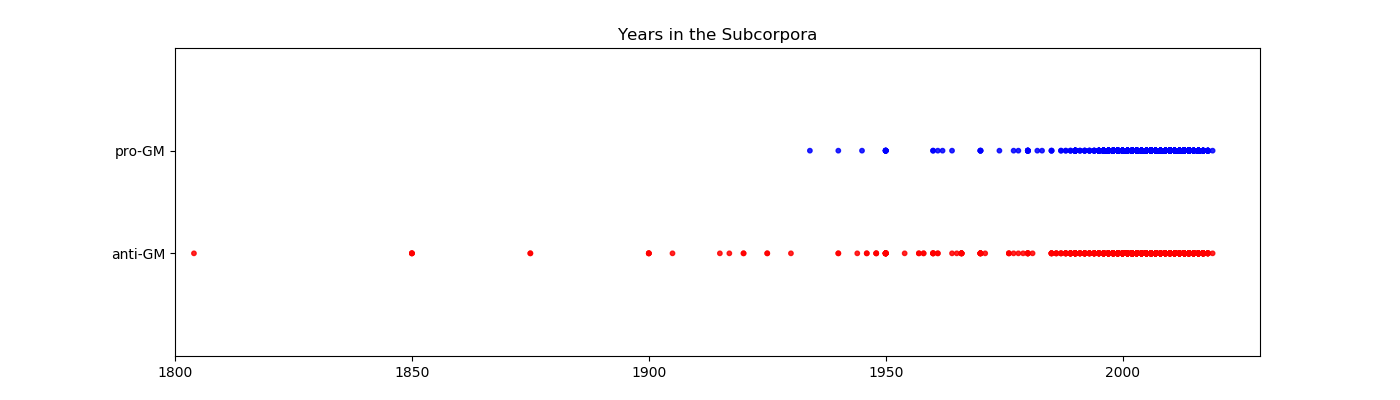
\includegraphics[width=16cm]{Figures/years.png}
\caption{Time horizons in the sub-corpora}
\label{fig:figure1}
\end{figure}

\textbf{Summary of the Cultural-Level}

By themselves, each observation at the cultural level does not lead to any conclusions. Taken together, however, the preceding results suggest that cultural difference is, indeed, a major factor in explaining diverging perspectives between the two sub-corpora. The first indication of cultural divergence is the very use of the term \textit{culture} in the anti-corpus and its relative absence from the pro-corpus. The fact that \textit{culture} appears much more in the anti-corpus and \textit{indigenous} is mentioned nearly 800 times, points to vastly different cultural contexts between the two sub-corpora. 

The geographic entity data suggest the anti-corpus contains a wider range of countries and cities. One could make the case, in turn, that this variety reflects a greater diversity of cultural perspectives. The same could be said for the temporal horizons. The wider span of years in the anti-corpus is suggestive that historical memory and context is at play to a greater degree.

\subsection{Socio-Economic Level}

Divisions in the GM-seed debate are deeply related to socio-economic imbalances and differing conceptions of economic growth. The 1950s and 60s saw the development of Green Revolution technologies (genetically modified/higher yielding crop varieties, synthetic fertilizer and pesticides, irrigation). The development of these technologies was followed by a neo-liberal policy framework in the 1970s and 80s, which (many argue) gave way to consolidation and monopoly control over agricultural supply chains. This included policies in the U.S., Canada and other developed countries that moved seed biotechnology from the public sector to the private seed industry. Vertical integration in agricultural supply chains accompanied horizontal consolidation of intellectual property rights for seed biotechnology. Rapid developments in genetic engineering and biotechnology took place in this economic context, leading to the situation today, where a handful of corporations control the majority of the world's seed markets and patents.

The controversy over GM-seed has coincided with neoliberal economic reforms. Free Trade Agreements (FTAs) have often granted legal intellectual property rights to international seed companies. The prohibition on seed saving can apply not only to patented varieties, but to any seed varieties that have not been registered or pre-approved. As a result, any farmer caught saving and replanting patented or even non-registered indigenous varieties could face fines or even jail time. There have been several cases where these laws led to nation-wide farmer's strikes and protests. For example, in June 2010, tens of thousands of Haitian farmers protested the ``deadly gift'' of seed to the Haitian government. After the devastating earthquake six months prior, smallholder farmers were faced with a shortage of seeds since many rural families used maize seed to feed the masses of refugees. In response, Monsanto (then the world's largest hybrid and GM seed company) announced it had delivered 60 tons of hybrid seeds of maize and vegetables; an additional 400 tons would be delivered throughout the year. Farmers would purchase these seeds from farmer association stores and the store revenue would be re-invested to purchase additional inputs of pesticides and fertilizers. The company itself acknowledged farmers would be unable to save and replant seed. This would potentially make farmers dependent on the market and purchased inputs.

Whether it's the Haiti case or elsewhere, economic analysis suggests that divisions over GM seed are not necessarily a consequence of biotechnology itself, but the economic context in which it has developed. In this for-profit context, purchased seed inputs are developed primarily to meet the circumstances of the largest customers (i.e. farmers with access to large acreages, machinery, credit, and subsidies). Pricing and regulations are established in the same vein. Also, seeking the largest return on investment, market-driven R\&D will naturally emphasize major crop varieties and sales volume, rather than specialty crops and fresh produce that suit local circumstances and small-producers.

The advantages commercial seed offers large-scale farmers do not necessarily translate to small producers and those in the certain parts of the world. For example, the labour-saving potential of GM crops presents a significant financial advantage to a farmer who otherwise would have to target-spray weeds with herbicide. With modern equipment and GM herbicide resistant crops, this farmer could do in hours what previously could take many days of work. The risk of crop failure is offset by insurance as well as government subsidy and income stabilization programs. In this case, planting large acreages with monocrop using commercial seed and chemical inputs, makes sense financially for producers.	

The economic context indicates how commercially patented seed may not fit the economic reality of many of the world's 800 million small-scale food producers. Consequently, those resisting the use of commercial seed varieties might be doing so as part of practical efforts to feed their families and earn a living. In other words, resistance is often based on lived realities faced by small-scale farmers in addition to cultural, ecological, or other factors.

\textbf{Concordances of \textit{Income}}

Here, we explore the hypothesis that economic factors discussed above are reflected in corpus data. The key terms analysis (Table 3.1) suggests that \textit{income} is a much more prominent concept in the pro-GM data. Frequency data further support this view. The word \textit{income} appears in the anti-GM corpus with a frequency of 0.22 per thousand words. In the pro- corpus the frequency is over eight times higher at 1.78. Tables 3.10 and 3.11 below show a sampling of 10 concordances of \textit{income} from both sub-corpora. The collocate \textit{farm income} accounts for the majority (174 of 237) of concordances from the pro-GM corpus. While this same collocate is present in the anti-GM corpus, it appears in only 2 (of 58) concordances.

The contrasting concordances are notable because the term \textit{farm income} is used in national and international policy discourse. In the concordances, the term is used at this higher-level of agricultural policy and economics, often accompanied by statistics spanning the entire sector. It is fair to say the term \textit{farm income} is associated with larger-scale commercial farming. By contrast, in the anti-GM corpus, the term \textit{income} is more likely to occur in the context of smaller-scale, household economics. Collocates \textit{community income}, \textit{household income}, or the possessive \textit{farmers' income} are all more prevalent. The lines refer to income in the context of local produce sales, and subsistence activities. Whereas the pro-GM corpus focuses on income gain and positive impacts, the anti-GM corpus refers more to losses, poverty, and scarcity.

\begin{table}[H]
\begin{footnotesize}
\centering
\begin{tabular}{c} 
\texttt{nology). The additional farm INCOME generated by the technology i} \\
\texttt{s up to 2004. Since then net INCOME gains fell to between \$3/ha a} \\
\texttt{ and \$18/ha. In 2014, the net INCOME gain was \$14/ha. The relative} \\
\texttt{ositive impact on direct farm INCOME in recent years reflects a co} \\
\texttt{997 there has been a net farm INCOME benefit from using the techno} \\
\texttt{f cost of 37 Increase in farm INCOME at a national level (\$ millio} \\
\texttt{tion of impact with yield and INCOME gains widely reported for man} \\
\texttt{rall, in 2014, the total farm INCOME from using the technology was} \\
\texttt{en to about \$20/ha. Net farm INCOME gains (after deduction of the} \\
\texttt{\ \ level is an increase in farm INCOME of \$2.5 million. Cumulatively}
 \end{tabular}
\caption{Concordance lines of \textit{income} Pro-GM corpus}
\label{tab:table1}
\end{footnotesize}
\end{table}

\begin{table}[H]
\begin{footnotesize}
\centering
\begin{tabular}{c} 
\texttt{nd an opportunity to generate INCOME by selling their produce at l} \\
\texttt{ definition of poverty as low INCOME . Poverty can mean the lack o} \\
\texttt{\ orted household and community INCOME generation. Extreme poverty h} \\
\texttt{o produce sufficient food and INCOME from locally-available resour} \\
\texttt{\ egular rather than occasional INCOME generation strategy. After th} \\
\texttt{ies to urban areas, household INCOME and use of non-traditional, p} \\
\texttt{\ \ prices, hurt local farmers' INCOME , and disrupted the usual pat} \\
\texttt{ese two GM crops deliver less INCOME on average to farmers than no} \\
\texttt{d rape sector in Canada; lost INCOME for organic and other GM-free} \\
\texttt{\ ut rather of lack of adequate INCOME to access food. In our countr}
 \end{tabular}
\caption{Concordance lines of \textit{income} Anti-GM corpus}
\label{tab:table1}
\end{footnotesize}
\end{table}

\textbf{Collocates of \textit{Corporate}}

Collocates of the word \textit{corporate} are also a telling indication of economic context in the anti-GM corpus. The corpus was searched for collocates that immediately followed the word \textit{corporate} (1R) and were repeated multiple times (minimum frequency 2). The result is a list with 12 collocations, 11 of which are in the anti-corpus (Table 3.12). These collocates include \textit{corporate control}, \textit{corporate power}, and \textit{corporate greed}. The pro-GM corpus contains only one multi-frequency collocate, \textit{corporate watch}. Many of these collocates are suggestive of an anti-GM discourse that views the topic of GM seed in terms of economic power relations. Some collocates (e.g., \textit{greed}) suggest a critical view of these relations. Other collocates of frequency 1 (not included in 3.12) confirm this critical view. For instance, included in the collocates are corporate \textit{interests}, \textit{lobby}, \textit{secrets}, \textit{evil}, \textit{control}, \textit{domination}, and \textit{shills}.  

The fact that anti-GM discourse is critical of corporate power is not, in itself, surprising. What is worthy to note, however, is that collocates of corporate are comparatively absent from the pro-GM corpus. Insofar as the pro-corpus discusses the topic in economic language, it seems to be in terms of increased efficiency, income, and profit, as reflected in Table 3.10. Economic power relations, it seems, are not discussed.   

\begin{table}[H]
\begin{footnotesize}
\centering
\def\arraystretch{1.1}% 
\begin{tabular}{ | m{2cm} | m{2.25cm} |}  
\hline
\textbf{Frequency} & \textbf{Collocate} \\
\hline
\multicolumn{1}{|c|}{12} & sector \\
\hline
\multicolumn{1}{|c|}{9} & control \\
\hline
\multicolumn{1}{|c|}{4} & seed \\
\hline
\multicolumn{1}{|c|}{4} & power \\
\hline
\multicolumn{1}{|c|}{3} & agriculture \\
\hline
\multicolumn{1}{|c|}{2} & takeover \\ 
\hline
\multicolumn{1}{|c|}{2} & subsidies \\
\hline
\multicolumn{1}{|c|}{2} & pressure \\
\hline
\multicolumn{1}{|c|}{2} & greed \\
\hline
\multicolumn{1}{|c|}{2} & finances \\
\hline
\multicolumn{1}{|c|}{2} & entities \\
\hline
\multicolumn{1}{|c|}{2} & consolidation \\
\hline
\multicolumn{1}{|c|}{2} & concentration \\
\hline
\multicolumn{1}{|c|}{2} & agency \\
\hline
\end{tabular}
\caption{Collocates of \textit{corporate} in the Anti-GM subcorpus}
\label{tab:table1}
\end{footnotesize}
\end{table}

\textbf{Income Split}

The previous analysis of country entities in the corpus suggests that a higher proportion of countries mentioned in the anti-corpus are from the Global South. This result points to possible economic differences between the two sub-corpora. To further explore this hypothesis, GDP data was used. All countries mentioned in the corpus (including city mentions) were ranked according to GDP (nominal) per capita. Among all countries, the average rank, average GDP, and percentages in the top and bottom quartiles (according to GDP), were determined. 

As Table 3.13 shows, all four data points suggest that the anti-GM corpus does indeed reflect lower income countries, though the significance of this difference is debatable. The average country rank (by GDP) is 11 percent lower in the anti-corpus; the average GDP is 8 percent lower; the percentage of countries in the top quartile by GDP is 9 percent lower; and the percentage of countries in the bottom quartile is 19 percent higher than in the pro-GM corpus. 

\begin{table}[H]
\begin{footnotesize}
\centering
\begin{tabular}{|l|l|l|}
\hline
\textbf{}            & \textbf{anti-GM} & \textbf{pro-GM} \\\hline
avg. rank            & 90                      & 81                     \\\hline
avg. GDP             & 20,766                  & 22,370                 \\\hline
\% in top quartile:   & 32                      & 35                     \\\hline
\% in bottom quartile & 38                      & 32                    \\\hline
\end{tabular}
\caption{Income data between the sub-corpora}
\label{tab:table1}
\end{footnotesize}
\end{table}


\textbf{Summary of Socio-Economic Level} 

The GDP statistics, together with the qualitative analysis of concordances of \textit{income}, are evidence that an economic divide exists between the pro and anti sub-corpora. Context of \textit{income} is drastically different between the two sub-corpora. On the one hand, \textit{income} is discussed in the context of profit, efficiency, and financial/capital gain. On the other, \textit{income} is mentioned in the context of subsistence/household economics and even economic hardship. Thus, while the term is central to both sub-corpora, it functions in entirely different contexts. 

The concordances are consistent with the GDP statistics, which give quantitative evidence that the anti-GM corpus is representative of lower income countries and regions. However, the GDP analysis overlooks the extent to which the economic divide might be intra- as well as international. In other words, country GDP data does not capture the extend to which the GM seed debate may be about dominant corporate entities vis-\`a-vis smaller-scale producers within countries.

Finally, the collocates of \textit{corporate} indicate that, not only is there an economic divide between the two sub-corpora, but that the anti-GM discourse is much more engaged in political/economic critique. 


\subsection{Cognitive Level}

The cognitive level aims to understand and compare the mental representations of language users in both sub-corpora. Elements of cognitive analysis of discourse, as outlined by \cite{VanDijk2000a}, include topics, implications, presuppositions, local coherence, and lexical meanings/connotations. Some of these elements have been covered, albeit not explicitly, in the other levels. For example, key word and key term analyses addressed \textit{topics}. Likewise, much of the collocation and concordance discussion relates to \textit{connotations}. 

In addition to elaborating on topics and connotations, this section looks at implication and presupposition. Coherence is examined through the notions of interdiscursivity and conceptual blending. 

\textbf{Implications and Presuppositions}

Implication pertains to cognitive analysis insofar as it contains socially shared knowledge that is inferred from explicit semantic contents of discourse \citep{VanDijk2000a}. Implicature \citep{Grice1975} is inferential and context dependent, that is to say, it relies on knowledge domains or mental schema. \cite{Sperber1995} make the distinction between `implicature' and `explicature', where (in explicature) assumptions are explicity stated. It may be the case that implications are understood more or less universally. It is also possible that implications rely on knowledge that varies across different cultures, communities of practice, or other groups. In such cases, implicature can be a reflection of ``cultural scripts'' \citep{Wierzbicka1985, Wierzbicka2003}.

Discourse is often full of implicature. From a corpus linguistic perspective, the challenge is narrowing the examples in a way that is consistent and comparable. Of course, identifying implicit assumptions by computationally searching a corpus is also a challenge.  In order to get a representative sample of implications in the corpus, we can look at collocates of the word \textit{means}, which is a common way to express implication in spoken and written English (i.e. A \textit{means} B). Although this relationship between A and B may be explicit, the assumptions underlying this relationship may not be.   

There are 81 and 43 such collocates in the anti- and pro-GM sub-corpora, respectively. The lines were manually and qualitatively analyzed and written in symbolic notation with a right arrow ($\rightarrow$) used to signify implication between propositions (e.g., A $\rightarrow$ B $\rightarrow$ C). The numbered segments below contain selected examples of implications in the pro-GM subcorpus, together with summarized implication relationships (in bold).

\begin{footnotesize}
\begin{quote}
\begin{enumerate}

  \item \texttt{Easier farming MEANS more food which, in turn, MEANS less expensive food.} \textbf{[Easier farming $\rightarrow$ more food $\rightarrow$ cheaper food]}\\

   \item \texttt{Decreased use of pesticides, MEANS less pesticide production demand and also less energy use on the farmers' end, too.}\\ \textbf{[Decreased pesticide use $\rightarrow$ less energy use]}\\
   
   \item  \texttt{Many plants are designed to use less pesticides and chemicals to grow, which MEANS less exposure to these potentially toxic substances for farmers and consumers.}\\ \textbf{[Less pesticides $\rightarrow$ less exposure to toxins]}\\
   
   \item  \texttt{Many GMOs are tailored for specific environmental conditions, which MEANS saving water in drought-prone areas and less use of chemicals.}\\ \textbf{[GMO seed $\rightarrow$ saving water AND less chemical use]}\\
   
   \item  \texttt{...GM [foods] have improved flavor and texture, as well as delayed ripening. This MEANS produce will stay fresh for longer periods of time.}\\ \textbf{[GMO seed $\rightarrow$ delayed ripening $\rightarrow$ produce stays fresh longer]}
  
\end{enumerate}
\end{quote}
\end{footnotesize}

The five examples above express relationships among different variables, such as food supply and food prices (1); pesticide use and energy use (2); pesticide use and toxins (3); genetic modification and water/chemical use (4); and genetic modification and preservation of freshness (5). Of interest, is the extent to which these relationships are explicit and quantifiable. Moreover, the logic of the relationships is more-or-less self explanatory as, for instance, the relation between food supply and food prices. In fact, in each example, the reader could conceive of a mathematical function depicting the relationship in question. Moreover, this relationship is often two dimensional; that is, between two variables (e.g. seed type and preservation time). Overall, little additional context is necessary to explain the relationships in question. Now, consider some examples from the anti-GM corpus:

\begin{footnotesize}
\begin{quote}
\begin{enumerate}

  \item \texttt{farmers...quickly lose control over seed management, production and eventually their land. This MEANS they lose their food sovereignty...} \textbf{[GM seed $\rightarrow$ loss of control over seed management $\rightarrow$ loss of food sovereignty}\\
  
  \item \texttt{...Monsanto (and other companies) own the rights to the modified DNA in their seeds. This MEANS farmers would have to buy seeds from them each year, and maybe more than once.} \textbf{[companies own seed rights $\rightarrow$ farmers have to buy seed annually]}\\
  
  \item \texttt{...they will cause reduced genetic diversity of plants and animals in the environment. What this MEANS is that the DNA, which codes for proteins in an organism, will become more similar between individuals of a species.} \textbf{[ reduced genetic diversity $\rightarrow$  loss of biodiversity]}\\
  
  \item \texttt{And if Paraguay is so dependent [on foreign companies] for such a basic thing as food...it MEANS that this is a subordinate country.} \textbf{[food dependence $\rightarrow$ national subordination ]}\\
  
  \item \texttt{...the nature of the promoter MEANS that the inserted genes are liable to be unstable and move out again.} \textbf{[promoter genes $\rightarrow$ instability in inserted genes $\rightarrow$ plant instability and variable gene functioning $\rightarrow$ unintended effects]}\\
  
  \item \texttt{...just three companies sell more than half the seeds on the market...this MEANS that the biological diversity of crops is declining, making our food supply less likely to adapt well to climate change.} \textbf{[three companies control seed market $\rightarrow$ declining biodiversity $\rightarrow$ less adaptive food supply]}\\
  
\end{enumerate}
\end{quote}
\end{footnotesize}

In comparison with the pro- examples, the implications above are not quantifiable. In many, cases the propositions cannot be expressed as variables; rather, the relationships involve implicit contextual or subjective factors that often evade objective representation. Consider the following relationships: GM seed and food sovereignty (1); food dependence and national subordination (4); and, biodiversity and adaptability of the food supply (6). In these cases, the relationship would be very difficult (if not impossible) to quantify. Moreover, an understanding of these relationships demands context based on an implicit set of factors/assumptions. 1 and 3, for example, invoke cascading sets of political/economic consequences induced by the adoption of GM seed by farmers, and culminating in loss of national sovereignty.     

In other cases, the relationships invoke biological complexity. In 5, the antecedent proposition (\textit{promoter gene}) leads to \textit{unintended consequences} via genetic instability. Similarly, in 6 the connection between seed market concentration, biological diversity, and ability to adapt to climate change depends on a complex set of factors.

Together, the implications observed in the corpus reinforce what is observed in the ecological level of analysis. Compared to the pro-subcorpus, the anti-GM discourse rests on mental models characterized by complex systems and conceptual schema that aims to encompass interrelations among multiple factors. Pro-GM discourse, by contrast, tends towards quantifiable relationships. 

\textbf{Interdiscursivity and Conceptual Blending}

The claim that anti-GM discourse operates in the context of more ``complex systems,'' is not meant to imply it is somehow more truthful or accurate. Rather, it is an attempt to characterize the conceptual and mental space within which the discourse operates. It is suggested that interactants in anti-GM discourse construct meaning by combining and mapping concepts from different mental spaces in ways that are not common in pro-GM discourse. Blending Theory \citep{Turner2002}, tells us that this combining and mapping of concepts gives rise to meaning as an emergent structure that is beyond the sum of its parts \citep[403]{Evans2006a}. While pro-GM discourse evidently employs conceptual blending in its own right, the results of preceding sections suggest that the emergent structure of the anti-GM discourse differs in the size and number of input spaces that contribute to an emergent structure of meaning. 

To pursue the basic idea that concepts are combined to form emergent meaning, we can consider interdiscourse as a particular manifestation of Blending Theory. Interdiscourse refers to the relations that a discourse has to other discourses. Drawing from \citep{Bullo2017a}, we propose that interdiscourse is part of a process of conceptual integration and sense making. As an example, we examine an excerpt from the anti-GM subcorpus. The following excerpt is from the ``Maize Manifesto'' released January 15, 2013 by the National Union of Autonomous Regional Peasant Organizations (UNORCA) in Mexico.

\begin{footnotesize}
\begin{quote}
\texttt{\justify In our country there are more than 60 native races and thousands of local varieties of maize, which instead of representing some kind of risk, carry important virtues thanks to their selection and adaptation by indigenous peoples over more than seven thousand years. Some of these native varieties offer higher yields than the ones manipulated by Monsanto. The imposition of transnational frankenseeds would mean an end to this richness and the loss of the ancestral milpa tradition as a sustainable system of maize production and symbol of the Mesoamerican cultural inheritance.}
\end{quote}
\end{footnotesize}

A high degree of interdiscursivity appears in this text. In this excerpt (and the Manifesto as a whole) the scientific discourse is not dismissed, but hedged as ``some kind of risk'' suggesting that, despite empirical research, there are unknowns associated with the technology. Scientific and technical aspects are explicitly acknowledged in this way, but are also implicitly placed in the framework of ancestral tradition and culture. Transitivity suggests interconnectedness and blurred boundaries between nature and culture. The notion of ``selection and adaptation'' of seed varieties over thousands of years suggests a natural attunement to complex biological processes, in contrast to an unnatural, hubristic ``manipulation'' of varieties by a large corporation. Similarly, the colonial, historical images could also work as a biological metaphor. The age-old Mayan milpa tradition of crop rotation and nutrient cycling being lost at the hands of a ``transnational'' seed is akin to an invasive species threatening an ecosystem. The historical context is also referred to in the use of the geographic term ``Mesoamerica'' (a cultural and bioregion) as opposed to the more historically recent nation states of the region. 

\textit{Frankenseeds} is itself an example of a type of conceptual blending known as compounding, whereby two or more morphemes combine to form a word \citep[415]{Evans2006a}. A subset of the meanings associated with each morpheme combines to give a unique and distinct meaning. The term \textit{frankenseeds} appears in both sub-corpora and is used among GM critics. Of course, the word invokes Shelly's Frankenstein, which is a portrayal of the dark side of industry and science as well as romanticism as a reaction to industrialization and Enlightenment disenchantment. Putting these literary themes in the context of GM seed is merely one example of how complex blending of concepts occurs in the excerpt and in GM discourse as a whole (Figure 3.2). 

To summarize, this excerpt demonstrates interconnectedness and layers of rich meaning that combine to form an emergent meaning that blends scientific worldviews, culture, nature, and history. 

\begin{figure}[H]
\centering
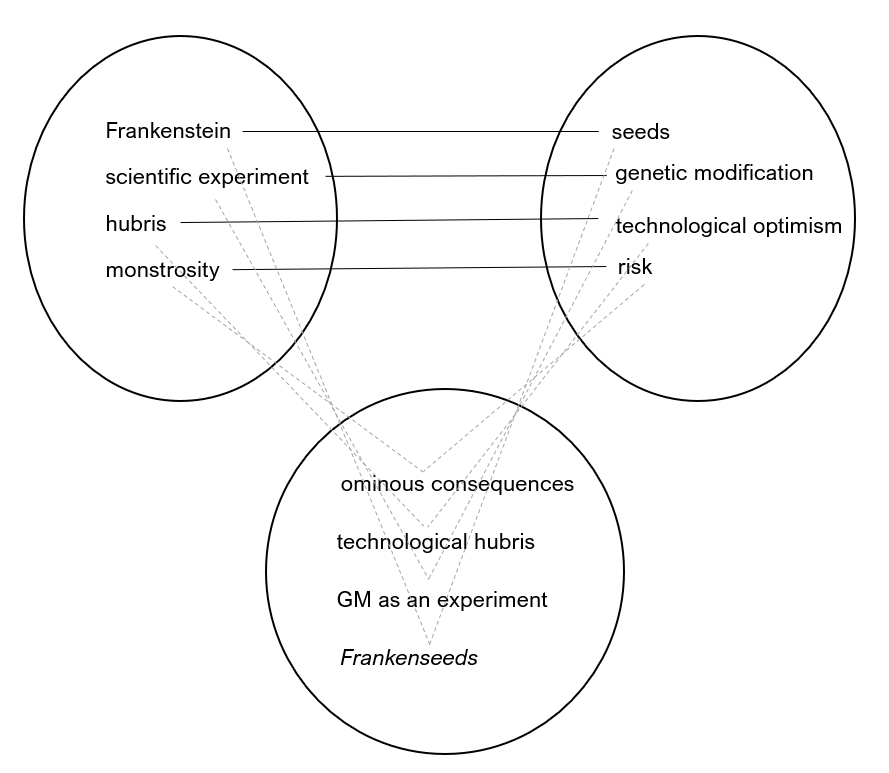
\includegraphics[width=8cm]{Figures/blending.png}
\caption{Compound blending to form \textit{Frankenseeds}}
\label{fig:figure1}
\end{figure}

\textbf{Situated Context}

In addition to blending of concepts within the corpus, we can also consider how non-discursive practices relate to the text. Such considerations are crucial at the cognitive level in light of situated cognition, or the premise that knowledge is inseparable from action. In other words, knowledge (and therefore discourse) is bound to social, cultural, and physical contexts \citep{Greeno1998}. The ``Maize Manifesto'' is not merely an article; rather, it is an political act that accompanied protests and hunger strikes by indigenous peasants in the Mexican capital. In short, the text is not understood in isolation, but in the situated context within which it was produced. 

The ``Maize Manifesto'' passage, together with results from the earlier section \textit{Specialization and Communities of Practice}, points to possible differences in extra-linguistic context between the sub-corpora. Specifically, we can consider that the anti-GM discourse takes place in the context closer to situated engagement with the topic, whereas as the pro- discourse is more likely to approach the topic through a third person, objective observer. Theoretical and empirical/scientific claims of pro-GM discourse contrast with the first-person lifeworld perspective of certain actors, such as those who produced the ``Maize Manifesto'' text. 

The essence of GM seed is often framed as a biological object. This is the logical result of a conceptual approach that presupposes a human as subject and the genetically altered organism as object. As such, discursive truth claims ultimately rest with those who possess specialized knowledge of this object relation (i.e. molecular biologists); those who take a third-person position over and against the object of study. In contrast, speakers in the ``Maize Manifesto'' begin with human experience and confront how GM technology is embedded in a plurality of contexts. 

\section{Summary \& Conclusions}

This chapter began by pointing out the complex nature of the GM seed debate. Through a multi-level analysis, the topic was broken down in order to view it from various perspectives. By splitting the corpus into two distinct sub-corpora, it was possible to gain insights into sources of misunderstanding and disagreement between sides of the debate. The following is a summary of findings:

\begin{itemize}
  \item Pro-GM discourse is significantly more likely to come from corporate or for-profit entities, while the anti-GM discourse is more likely to originate from non-profit or advocacy organizations. 
  \item Anti-GM discourse contains culturally significant key words and key phrases while those in the pro-GM discourse are more technical and specialized. 
  \item Concordance analysis also suggested \textit{culture} is a far more prominent factor in the anti-GM discourse.
  \item Anti-GM discourse is more likely to view natural systems holistically whereas the pro-GM discourse takes a more analytic and reductionist approach.
  \item The countries mentioned in the corpus are more distributed in the anti-GM subcorpus.
  \item Based on years and decades mentioned, the temporal span in the anti-GM corpus is larger.
  \item Concordances of \textit{income} suggest the economic context in the sub-corpora is different, with the anti-subcorpus focused more on economic scarcity and household income as opposed to the term \textit{farm income} in the pro-subcorpus.
  \item Based on collocates of \textit{corporate}, the anti-GM discourse is more critical of socio-economic structures.
  \item Analysis of the country data suggests that lower income countries are more represented in the anti-GM corpus.
  \item Analysis of implications suggests the pro-GM subcorpus explains relationships in more quantifiable variables, whereas the anti-subcorpus contains more qualitative, subjective, and unquantifiable relationships.
  \item Interdiscursivity, conceptual blending, and situated context all seem to be markedly different between the two sub-corpora.
\end{itemize}

Before drawing any conclusions from these findings it is important to point out an underlying assumption; namely, that the corpus is representative of GM seed discourse. Assuming the corpus does, to a significant extent, represent the societal discourse on the topic, the multi-level results are significant. Taken alone, each of the above results is not telling. However, taken together, the above findings point to crucial differences between the two sub-corpora and, hence, between the two sides of the GM seed debate.

The results suggest that the anti-GM discourse embodies a plurality of actors in a way that the pro-GM discourse does not. This plurality is suggested in the distribution of countries/geographic entities in the corpus as well as the cultural context of the anti-GM subcorpus. In addition, the cognitive analysis indicates that intersubjectivity, or psychological connotations/first-hand experiences with respect to GM seed, is an undercurrent in the anti-GM discourse. Intersubjectivity is itself an expression of plurality, insofar as it is the coming together of diverse human subjects. This intersubjective orientation is in contrast to the third-person, subject-object perspective pro-GM discourse. 

The plurality inherent in anti-GM discourse points to a possible source of misunderstanding between different sides of the debate. In the face of the complex web of relationships and perspectives, people may attempt to organize and categorize the discourse into familiar categories and frames. Cognitively, this categorization functions similar to stereotype, where information is simplified in order to make sense of an otherwise too complex world \citep{Tajfel1981}. No doubt, this simplification is inevitable in the face of a complex topic such as GM seed. However, the condition of plurality in the anti-GM discourse makes this side of the debate particularly susceptible to reduction and simplification on the part of their critics.

In order to see this simplification at play in GM seed debate, consider the following excerpt from the pro-GM subcorpus. The excerpt is from the article ``The Truth about Genetically Modified Food'' by David H. Freedman in the August, 2013 issue of the magazine \textit{Scientific American}. 

\begin{footnotesize}
\begin{quote}
\texttt{\justify Some scientists say the objections to GM food stem from politics rather than science\textemdash that they are motivated by an objection to large multinational corporations having enormous influence over the food supply; invoking risks from genetic modification just provides a convenient way of whipping up the masses against industrial agriculture. "This has nothing to do with science," Goldberg says. "It's about ideology." Former anti-GM activist Lynas agrees.  He recently went as far as labeling the anti-GM crowd "explicitly an antiscience movement."}\\

\texttt{It is also true that many pro-GM scientists in the field are unduly harsh\textemdash even unscientific\textemdash in their treatment of critics. GM proponents sometimes lump every scientist who raises safety questions together with activists and discredited researchers.... Most of them are nonscientists, or retired researchers from obscure institutions, or nonbiologist scientists....}
\end{quote}
\end{footnotesize}

The dominant frame in this text is that of empirical science, specifically peer reviewed research in a setting of certain prestige Anglo-American institutions. Alternate social and institutional meanings are secondary, if at all considered. The article as a whole does raise the concern of perceived influence of industry funding on research perspectives. Also, possible unknowns inherent in the scientific research are pointed out. However, there is an ordering of discourses below the scientific. In an apparent representation of both sides of the debate, the possible flawed (``unduly harsh\textemdash even unscientific'') position of some GM proponents is not a result of their failure to consider alternate discourses, but that they ``lump'' otherwise objective scientific concerns together with non-scientific perspectives of ``activists and discredited researchers.'' In other words, the pro-GM argument would be even stronger if they ignored non-scientific discourses all together. These non-scientific perspectives include those related to politics, corporate influence, industrial agriculture; those advanced by activists, nonbiologist scientists, or researchers at ``obscure institutions.'' Identity construction and word choice (``masses,'' ``crowd,'' ``activists,'' ``obscure,'' ``retired,'' ``ideology,'' ``discredited'') are used pejoratively in contrast to seven instances where ''science'' has an unreservedly positive connotation.

The excerpt above is an example of how the plurality of perspectives of GM critics is framed in a simplified manner. In fact, in this excerpt the other side of the debate is characterized maintaining the same frame as was used to reinforce the pro-GM perspective. From the multi-level analysis we see that the pro-GM discourse is more focused on empirical science, analysis, and reduction of complex systems. In the excerpt, these same methods are used to characterize/critique the other side of the debate. However, the multi-level analysis suggests that an understanding of the anti-GM discourse requires entirely different modes of understanding. The anti-GM discourse is based on epistemological as well as cultural, political-economic, and even cognitive factors, the understanding of which requires consideration of multiple-levels and perspectives. Approaching the debate without full consideration of its multi-level nature inevitably leads to misunderstanding.  % Analysis 1

\chapter{Analysis 2: Verbal Communication \& the Dakota Access Pipeline}
\lhead{\textit{Analysis 2: Verbal Communication \& the Dakota Access Pipeline}}

\textit{\textbf{Chapter Summary:} This chapter examines verbal communication (in the form of quotations from texts) in relation to the Dakota Access Pipeline. Segmenting speakers into three groups allows for comparative analysis showing how actors in the debate employ different keywords and connotations. Crucially, patterns of cultural discourse and stereotyping can be identified.}
\newline

\section{Background}

In August 2016, Indigenous protesters chained themselves to heavy machinery in North Dakota. In the following months, viewers worldwide saw protesters arrested, attack dogs unleashed, encampments bulldozed, and the heavily armed National Guard march in to the otherwise peaceful grasslands of Sioux County. At issue was the construction of the Dakota Access Pipeline, a \$3.8 billion project, proposed by the Dallas-based Fortune 500 company Energy Transfer Partners, which would transfer shale oil from the Northern Plains to the industrial heartland (Figure 4.1). The previous chapter approached the theme of GM seed through high level textual analysis. This chapter looks at a more localized environmental issue and by examining statements made by specific speakers. Here we are concerned with the debate surrounding the Dakota Access Pipeline as expressed in quotations by various stakeholders. 

Any analysis of communication surrounding the Dakota Access Pipeline (DAP) will have to account for diverse perspectives. Infrastructure and resource projects, as well as environmental issues in a broader sense, precipitate a complex dynamic of conflicting ideas, worldviews, and values. In the case of the DAP, this dynamic included spiritual values of the Native American Sioux; historical land disputes; issues of inequality and corporate power; science and engineering practice; local/national politics, and global environmentalism. 

For any project of this scale, there are voluminous communication artifacts one could analyze, ranging from court records and environmental assessments to news articles and social media posts. Having gained national and international headlines, the Dakota Access Pipeline resulted in an even greater volume of communication than is typical for such a project. As protests escalated through the fall months of 2016, the cause garnered support from outgoing President Obama and presidential candidate Bernie Sanders. Sioux leader David Archambault II brought the issue before the UN Human Rights Council in Geneva. This was followed by the UN Special Rapporteur on the rights of indigenous peoples calling for a halt to construction, stating that the Standing Rock Sioux tribe had been ``excluded from consultations'' \citep{OHCHR2016a}. In January 2017, as one of his first executive actions, the newly elected President Trump directed the U.S. Army Corps of Engineers to approve the pipeline in an ``expedited manner'' \citep{OfficeofthePressSecretary2017a}. Within weeks, authorities cleared out the last remaining protest camps and construction crews began drilling. By June, the oil was flowing. 

The protests drew international attention and reshaped the national conversation about resource projects on Native American land \citep{Liu2013a}. The fact that the protest site became the largest gathering of Native Americans in over 100 years \citep{Northcott2016a} puts the events in the context of deep and ongoing historical struggles for indigenous sovereignty and decolonization. 


\begin{figure}[H]
\centering
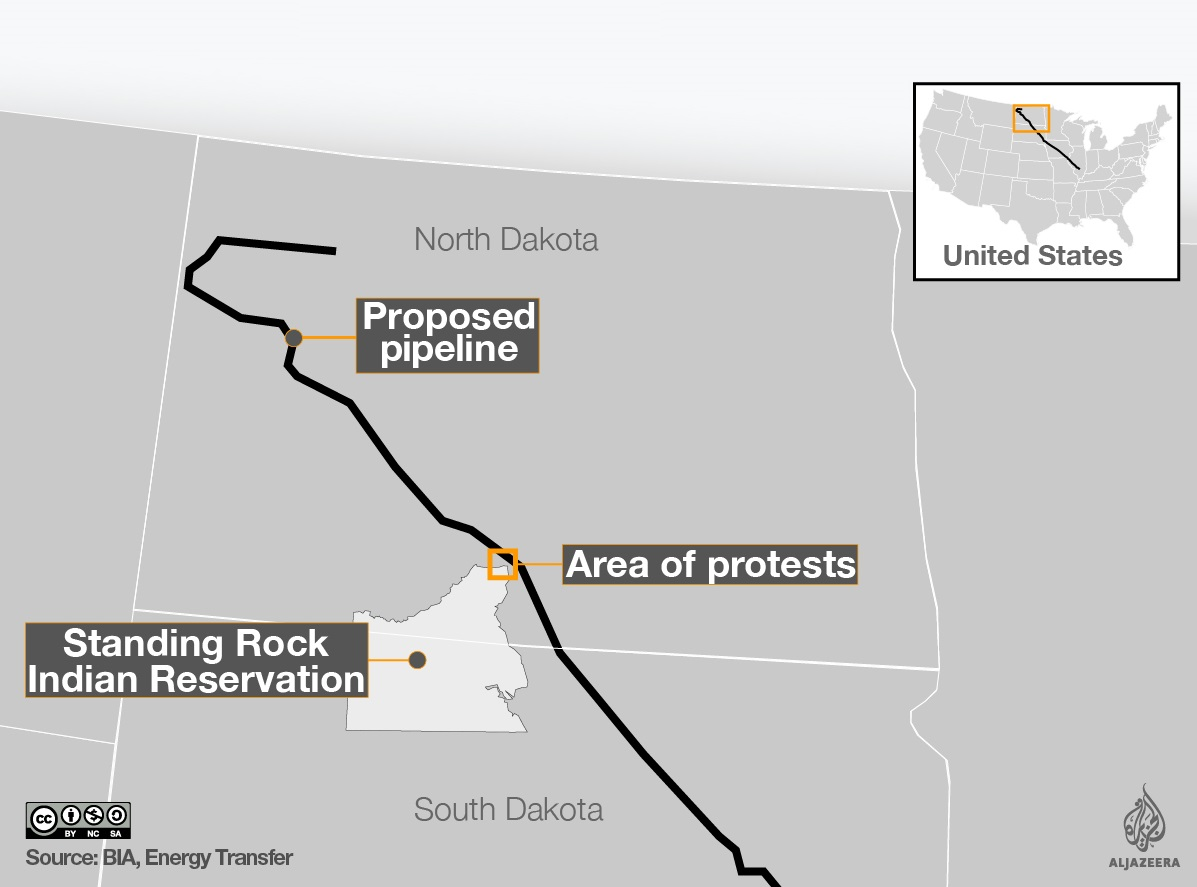
\includegraphics[width=9cm]{Figures/dakota.jpg}
\caption{Dakota Access Pipeline route}
\begin{footnotesize}
Creative Commons image from https://www.aljazeera.com
\end{footnotesize}
\label{fig:figure1}
\end{figure}

The challenge in describing communication surrounding this issue, is largely methodological. Disparate and voluminous data must be gathered and analyzed at a manageable scale, while also accounting for a breadth of sources and perspectives. Difficulties in scope and framing also become apparent when faced with methodological choices. At its core, one could argue, the pipeline is strictly a scientific and engineering problem. From another perspective, one could make the case that the issue is best approached in terms of power and class. Looking at discourse surrounding the issue also makes it clear that culture, specifically indigenous identity, is central to this issue. Even the time horizon is not entirely clear. Whereas the issue explicitly began in June 2014 (when the project was announced), one could also argue that it reaches back over 150 years ago with the Treaty of Traverse des Sioux (1851) and the Treaty of Fort Laramie (1868), when the U.S. Senate ratified treaties that recognized the Sioux peoples' national sovereignty. What follows is a multilevel framework for integrating the disparate aspects of the pipeline debate. 

\section{Corpus Data}

This second corpus corresponds to the verbal level and contains quotations related to the Dakota Access Pipeline. To build this corpus, quotations were collected from online articles. Granted, quotations from articles do not achieve the depth of primary sources and ethnographic interviews. However, there are several advantages of drawing from quotations in this way. Assuming that principles of responsible journalism were followed, quotations are accurate and reliable; they contain the original spoken words and editing will not have changed the meaning of statements \citep{CAJ2011a}. Collecting quotations also allows for large-scale data analysis and presentation of diverse perspectives.	

First, a corpus of articles was made by conducting an online search from two queries: ``Dakota Access Pipeline,'' ``Dakota Access pipeline AND protests.'' The result was 226 pages with a total word count of 300,000. Quotations were then extracted from the corpus using regular expression matching. 500 characters before and after each quotation were also extracted so, for each quote, the context as well as the speaker could be identified. 

The result was 628 quotations with contextual text snippets. After manual analysis, the list of 628 was reduced to 388 by balancing the speakers/perspectives and consolidating where there were several successive quotes by one speaker. A speaker was then assigned to each quotation, including a name as well as any other identifying information contained in the contextual snippets, such as occupation, origin, ethnicity, or institutional affiliation.

Once quotations were obtained, they were read (in context) and categorized according to the identities/stance of the speakers. Broadly speaking, speakers fell into one of three categories: (i) proponents of the pipeline; (ii) protesters/citizens directly opposing the pipeline; and (iii) people lending support for the cause of the protesters but not protesting in a direct manner. For the purposes of this analysis, the focus is on categories (i) and (ii), proponents and opponents. The quotations were then grouped according to the stance of the speakers as well as context of the statements (Figure 4.2). Quotes from proponents (i.e. quotes made in the context of advocating for the pipeline or denouncing the protesters) were put into Group A. Groups B and C both contain quotes from pipeline opponents/protesters. Group B contains quotes that related to rights, justice, and equality. Group C is reserved for quotes more explicitly expressing culture and identity.  

\begin{itemize}
  \item \textbf{Group A}: Proponents who either actively voiced support for the pipeline (e.g. company representatives) or took a legal or institutional stand against the pipeline protesters (e.g. law enforcement)
  \item \textbf{Group B}: Protesters/opponents raising issues of trust, fairness, or inequality (e.g. rights to land, oppression of law enforcement)
  \item \textbf{Group C}: Protesters/opponents expressing cultural identity, such as group membership or cultural assertions (e.g. values, worldviews, ethnic/linguistic identity)
\end{itemize}

\begin{figure}[H]
\centering
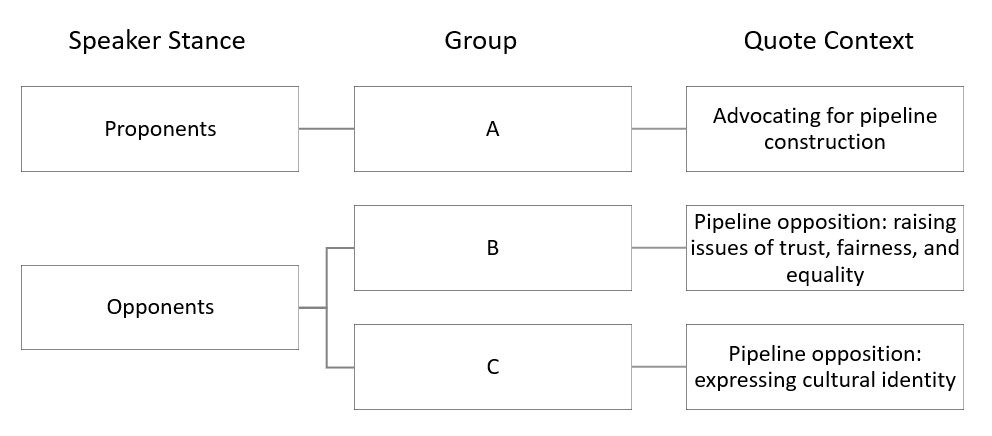
\includegraphics[width=13cm]{Figures/groups.png}
\caption{Groupings of quotations}
\label{fig:figure1}
\end{figure}

\section{Multilevel Analysis}

Multilevel analysis can help us understand a complex topic like the DAP. The issue is obviously and, perhaps most explicitly, ecological. The cultural aspects of the DAP are also explicitly expressed by the indigenous stakeholders. However, the data suggest socio-economic factors also pervade the issue, albeit these factors are often expressed more indirectly in comparison with the ecological and cultural levels.

Compared to Analysis 1, this analysis relies on more manual and qualitative methods. Focusing on quotations allows for this manual analysis, since the corpus is reduced to a manageable size. Most importantly, focusing on quotations is a way to associate specific statements with specific speakers and their identities\textemdash something that would not be possible with the corpus in the previous chapter (Analysis 1).  

At the level of verbal quotations, the overlap between the different levels of analysis becomes apparent. In other words, it becomes clear that the ecological, cultural, socio-economic, and cognitive levels are not distinct categories. In fact, one single statement might span all or several of these levels. However, categorizing and grouping the quotations is a way to clarify the levels and their interrelation.

One might question the decision to separate a subset of quotations as `cultural'. The implication, of course, is that certain statements are not cultural, contradicting the notion that culture is everywhere and pervasive is all human communication. However, based on the distinction (from Chapter 2) between culture and civilization, we are proposing that some utterances are, indeed, more cultural than others. For instance, we see that, in comparison with Group C, Group A does not contain cultural meanings such as personhood, relationships, or identity.

\textbf{Keyword Analysis}

Keyword analysis points to dominant themes in each group. Quotes were processed by removing punctuation, cases, symbols, and stop words as well as performing stemming and lemmatization. For each of the 3 groups, the top 20 keywords were then obtained based on frequency (Table 4.1).  

Keywords in Group A such as \textit{law}, \textit{state}, \textit{federal}, \textit{company}, and \textit{police} are indicative of discourse related to institutions. It is also relevant to note that \textit{protester} is the second most common term in Group A, whereas it does not appear in the other groups. A possible explanation is that \textit{protester}, with pejorative undertones, is part of identity construction and `othering' rather than a term people use to describe themselves. The terms \textit{behavior}, \textit{aggressive}, and \textit{safety} also point towards possible negative portrayals of citizens opposing the pipeline. Finally, it might be noted that the only apparent environmentally-related term in Group A is \textit{energy}, which is a dominant theme of the pro-pipeline side (i.e. \textit{energy} independence, \textit{energy} infrastructure, \textit{energy} security).  

In Group B keywords, cultural language begins to emerge with \textit{nation}, \textit{indigenous}, or \textit{Dakota}. Through \textit{right}, \textit{government}, and perhaps \textit{force}, one can see evidence of the rights-based or anti-oppression discourse. This is expected since the category contains quotes related to issues of trust, fairness, and equality. The keywords \textit{land} and \textit{water} indicate the ecological thrust of this group, whereas the absence of \textit{energy} contrasts with that of Group A. Group C keywords bring the cultural themes into more focus. Along with \textit{indigenous}, this group features the words \textit{prayer}, \textit{sacred}, and \textit{human}. In addition to \textit{water}, the ecological-related keywords in Group C include \textit{earth} and \textit{life}.   

\begin{table}[H]
\begin{footnotesize}
\centering
\begin{tabular}{|l|l|l|l|l|l|}

\hline
\multicolumn{2}{|l|}{\textbf{Group A}}           & \multicolumn{2}{l|}{\textbf{Group B}}            & \multicolumn{2}{l|}{\textbf{Group C}}            \\ \hline
\textit{\textbf{Word}} & \textit{\textbf{Freq.}} & \textit{\textbf{Word}} & \textit{\textbf{Freq.}} & \textit{\textbf{Word}} & \textit{\textbf{Freq.}} \\ \hline
pipeline              & 5                       & people                 & 9                       & people                 & 13                      \\ \hline
protester                 & 4                       & nation                 & 6                       & going                  & 10                      \\ \hline
energy                    & 4                       & iowa                   & 6                       & camp                   & 8                       \\ \hline
law                  & 4                       & indigenous             & 5                       & water                  & 7                       \\ \hline
state               & 3                       & dakota                 & 5                       & protect                & 7                       \\ \hline
transfer                & 3                       & government             & 5                       & pipeline               & 6                       \\ \hline
partner                & 3                       & right                  & 5                       & prayer                 & 6                       \\ \hline
federal                 & 3                       & water                  & 4                       & right                  & 6                       \\ \hline
people                  & 3                       & project                & 4                       & something              & 6                       \\ \hline
think                 & 3                       & going                  & 4                       & fight                  & 5                       \\ \hline
others                & 3                       & land                   & 4                       & life                   & 5                       \\ \hline
company               & 3                       & trying                 & 3                       & indigenous             & 5                       \\ \hline
behavior                 & 2                       & would                  & 3                       & future                 & 5                       \\ \hline
safety                 & 2                       & say                    & 3                       & sacred                 & 4                       \\ \hline
caused                 & 2                       & industry               & 3                       & think                  & 4                       \\ \hline
police                   & 2                       & get                    & 3                       & human                  & 4                       \\ \hline
said             & 2                       & far                    & 3                       & need                   & 4                       \\ \hline
aggressive                  & 2                       & pipe                   & 3                       & mother                 & 4                       \\ \hline
would                 & 2                       & force                  & 3                       & earth                  & 4                       \\ \hline

\end{tabular}

\caption{Keywords from each group of quotations}
\label{tab:table1}
\end{footnotesize}
\end{table}

\subsection{Ecological Level}

Picking up on the keyword analysis, this section looks closer at the ecological themes in the quotations. The environmental debate surrounding the Dakota Access Pipeline spans local, national, and global dimensions. Pipeline opponents allege the pipeline's crossing of the Missouri River constitutes a threat to the region's clean water. However, more global issues, notably climate change, are also key motivations for resistance. Project proponents, on the other hand, often cite the relative safety of pipeline transport vis-\`a-vis the alternatives. The theme of national energy independence and energy security is also advanced by proponents. 

It is important to note that, although the pipeline is clearly a topic of environmental debate, ecological topics are not central to the quotations. In Group A, for instance, there are 23 quotations and only 2-3 explicitly address the environmental issues. 

In addition to direct ecological-level considerations, this section discusses the relation between environmental issues and other themes in the discourse. As in Analysis 1, we consider how the environment is framed. The quotations give indications of how the natural world is construed by different actors. 

\textbf{Group A: Discourse of Security}

In Group A, the environment is framed through projects and infrastructure. The natural world is spoken of in terms of resources and management. Consider the following statements by the company proposing the project.

\begin{footnotesize}
\begin{itemize}
\item[] \texttt{[We] developed response and action plans, and will include several monitoring systems, shut-off valves, and other safety features to minimize the risk of spills....\newline \textit{-Energy Transfer Partners spokesperson}} 
\newline
\item[] \texttt{[the project meets] all applicable federal, state and local environmental laws, regulations and standards.... We continually seek ways to enhance our operations in the areas of environmental and resource protection and conservation.\newline \textit{-Energy Transfer Partners spokesperson}} 

\end{itemize}
\end{footnotesize}

The first statement frames the physical environment as something that can be managed and controlled through technology. The second statement also refers to management, albeit in the context of laws and regulations as opposed to technology. Both statements refer to the natural world through human intermediaries and institutions. No doubt, they are intended to convey an impression of competence and control with respect to the built, physical environment.

Aside from statements about managing risks, proponents also make the case for the pipeline as needed energy infrastructure. The following statement from Group A typifies this position:

\begin{footnotesize}
\begin{itemize}
\item[] \texttt{We think this is a great step forward for energy security in America.\newline \textit{-President of the North Dakota Petroleum Council}}
\end{itemize}
\end{footnotesize}

This quote indicates the national geographical focus (i.e. \textit{America}) that is common in the proponents' discourse. While the opposition discourse also has national references, the focus is on local/regional environmental impacts (e.g. risk of water contamination) as well as the global-level (e.g, climate change). Although local jobs are also a factor, the project being in the national interest is a key argument among proponents.  

The word \textit{security} is notable in the quote above. As the keywords indicate, \textit{security} (in the sense of law and order) is a reoccurring theme in Group A. In the quote above and in the text data as a whole, we see this theme extends to the ecological realm with the notion of \textit{energy security}. This suggests that discourses of public safety and national security are intertwined with those of environmental and resource security. In both cases, there is a perceived threat (e.g, energy insecurity, dependence) together with a set of actions to confront that threat. 

From a discourse analysis perspective we might also consider how \textit{security} functions in order to justify and legitimize certain actions that may be outside of the norm. For example, using a corpus of documents from security organizations, \cite{MacDonald2019} posit that \textit{security} functions to construct a state of exception while (seemingly) adhering to liberal-democratic principles. Likewise, the notion of \textit{energy security} might mobilize a discourse whereby the pragmatic ends of national interest and cheap energy are used to counter environmental concerns. In other words, if environmentalism itself creates a state of exception (e.g. to justify civil disobedience), the discourse of \textit{security} is a response that invokes economic and national interest.

\textbf{Group B: Discourse of Environmental Justice}

Insofar as quotations in Group B concern the ecological-level, they are often more political in nature. For instance, a number of speakers address the perceived conflict of interest among regulators and the oil and gas industry. At this ecological-level of analysis, we note how the environment emerges as the cite of political/economic injustice. In particular, infrastructure is seen as reflecting power dynamics of the broader society and resisting projects is a way to resist perceived injustices in those dynamics. The following quotes reflect this sentiment:  

\begin{footnotesize}
\begin{itemize}
\item[] \texttt{North Dakota regulators are really, I would say, in bed with the oil industry and so they have looked the other way.\newline
\textit{-Winona LaDuke, Ojibwe activist and Green Party candidate}}
\newline
\item[] \texttt{...big business and big ag are pulling the levers of government in Iowa.
\newline
\textit{-Adam Mason, Iowa Citizens for Community Improvement}}
\end{itemize}
\end{footnotesize}

Similarly, consider the following quote by a citizen who came to the protests from Flint, Michigan. The speaker is referring to the \textit{Flint water crisis} where, due to mismanagement by regulators and cost-cutting measures, drinking water was contaminated in the city of Flint.\footnote{The Flint water crisis started in 2014 when officials failed to apply corrosion inhibitors to the water. As a result, lead from aging pipes leached into the water supply, exposing over 100,000 Flint, Michigan residents to elevated lead levels.} 

\begin{footnotesize}
\begin{itemize}
\item[] \texttt{We know in Flint that water is in dire need,... In North Dakota, they're trying to force pipes on people. We're trying to get pipes in Flint for safe water.}
\end{itemize}
\end{footnotesize}

Whereas Group A clearly contains statements intended to convey management competency and legitimacy over natural resources, statements from Group B challenge the legitimacy of regulators and industry. Given these themes, Group B is discussed in more detail in the later socio-economic level of analysis. The crucial point here, however, is that speakers in Groups A and B form a coherent discourse between them, at least with respect to ecology and environment. In other words, there is an extent to which the discourses of Groups A and B are in dialogue with each other. The points made by each side have a common context and framework for meaning. The language is that of legitimacy/governance over resources and infrastructure. By contrast, in the next section we consider how, in Group C, ecological language is part of an entirely different framework of meaning.  

\textbf{Group C: Environment and Cultural Identity}

In Group C, references to the natural world are made in the context of cultural identity, values, and human well-being. In various quotes, the notion of culture is emergent in the sense that it results from the interplay of different elements, including the natural world. In contrast to Groups A and B, the environment is not framed through infrastructure and resources; rather, it takes on a more intrinsic value. There is a notable contrast with Group A where there is an analytical approach to the environment as something to be managed. Group C, by contrast, contains more holistic views of relationships and interactions with the environment. The following quote is an example: 

\begin{footnotesize}
\begin{itemize}
\item[] \texttt{We are going to keep it going, keep organizing meetings and find a way to be able to take care of the health and welfare of our people, and preserve land and water.   \newline
\textit{-Ivan Lookinghorse, Cheyenne River Reservation}}
\end{itemize}
\end{footnotesize}

By juxtaposing health and welfare with ecological preservation (as opposed to speaking in strict cause and effect terms), the speaker invokes a complex set of relationships and interactions. Here, the cause and effect relationship between the environment and human health is present, but the case for ecological preservation is not reducible to human health. In other words, there is cultural value\textemdash as opposed to strictly utility value \textemdash placed on preservation. The following quote also points to complex interactions between the environment and the economic, political, and cultural spheres:

\begin{footnotesize}
\begin{itemize}
\item[] \texttt{...in peaceful prayer and in dignity as we assert our rights to protect our environment, our economy and our sovereignty.   \newline
\textit{-Chase Iron Eyes, activist}}
\end{itemize}
\end{footnotesize}

The possessive pronoun \textit{our} clearly indicates the speaker is invoking cultural identity. Crucially, this identity entails a holistic relationship between the environment and economy. Contrast this with Group A, where the national economy (i.e. energy security and national interest) is invoked to defend pipeline construction. The emphasis on relationships is also apparent in following quote: 

\begin{footnotesize}
\begin{itemize}
\item[] \texttt{We're here today to send a message that we, as human beings, are indigenous to the earth. The earth is our mother. Your relationship with the mother is forever. The earth gives us our water, our air, our food, our shelter. We need to protect it.  \newline
\textit{-Cassandra Begay, a member of the Navajo tribe}}
\end{itemize}
\end{footnotesize}

This is one of a number of quotations in Group C that use personification of earth as \text{mother} as an embodiment of life-giving and nurturing aspects of nature. Even though the last part of the example (``The earth gives....'') could be said to refer to the utility value of nature, the \textit{mother} metaphor frames nature in a way that transcends any means-ends, utilitarian representations. 

As in Analysis 1, depending on the context, we see stark contrasts between the way in which nature is referred to. In Group A, nature is framed in a physical, commodity-based manner. Speakers reference management of specific systems of infrastructure and materials as opposed to holistic interactions and intrinsic value. Group B maintains this framing, insofar as speakers are challenging the legitimacy to jurisdiction over materials and energy. 

In Group C, nature is takes on an entirely different frame of meaning. It is part of holistic relationships and interactions with people, culture, and the economy. It is in this sense that speakers in Group C are communicating within an entirely different framework that integrates layers of meaning, including cultural/spiritual expression. 
  
\subsection{Cultural Level}
Indigenous communities are, of course, the predominant cultural groups affected by the pipeline and involved in the protests. A key question, then, is how the discourse is reflective of these communities, or how analogous observations apply to other identifiable groups. Of course, this presupposes that we can indeed identify speakers as members of distinct groups. In other words, we first need to inquire as to how group identities are expressed and constructed. 

Distinguishing between cultural groups or speech communities carries the risk of essentializing identities \citep{Dervin2016a, Piller2007a} or stereotyping `the other' \citep{Fedor2014a}. At the same time, these very group identities are also rich, meaningful aspects of experience and selfhood. It is important, therefore, to distinguish between instances where speakers identify themselves as members of cultural groups versus instances where an identity is assigned/constructed by others in the society. The present analysis looks at cultural identities that are explicitly expressed by speakers. In other words, we are interested in cultural indicators in communication, such as group membership, pronoun usage, or other markers of identity. 

We can also distinguish between expressions of self identify versus cases where an identity is assigned/constructed. In other words, of interest are both self expression of identities (e.g. ``\textit{we} are indigenous'') as well as cases where identities are applied to others (e.g. ``\textit{they} are eco-terrorists''). The latter often involves othering. Othering involves defining a person or group in a negative way that creates distance and difference \citep{Powell2017}. Here we argue that othering is a process of stripping away culture; it is the antithesis of intercultural communication in the sense that a cultural group is labelled or outright denied, rather than understood in familiar terms.  

\textbf{Othering as Negation of Culture}

In the source quotations, the theme of culture does not occur until groups B or C. Cultural groups are scarcely mentioned in Group A. One could question the overall significance of the absence of culture in Group A, and the degree to which this absence is an intended feature of discourse of pipeline proponents. 

Rather than through cultural identity, speakers in Group A refer to protesters in the negative terms of othering. Consider the following segments from Group A:

\begin{footnotesize}
\begin{itemize}
\item[-] \texttt{Protesters' escalated unlawful behavior}
\item[-] \texttt{[protesters had been] very aggressive}
\item[-] \texttt{eco-terrorist groups}
\item[-] \texttt{the anti-DAPL diaspora}
\item[-] \texttt{these things can be overwhelmed from outside groups}
\item[-] \texttt{a large component is very violent, very confrontational}
\item[-] \texttt{There is an element there of people protesting who are frightening. It's time for them to go home.}
\end{itemize}
\end{footnotesize}

Rather than referring to the protesters as identifiable people, they are anonymized as ``protesters'' or ``groups.'' Despite the fact that the protest camp was established by local Standing Rock Sioux tribal citizens, statements by pipeline proponents scarcely mention this group or other indigenous communities. In fact, phrases such as ``diaspora'' or ``outside groups'' create the image of geographically dispersed individuals with no local ties or history. In addition, protesters are characterized as ``unlawful,'' ``aggressive,'' ``violent,'' ``confrontational,'' and ``frightening.'' These adjectives disassociate protesters from society. Crucially, this disassociation is not made through cultural difference. Instead, it coincides with the rendering of protesters as an anonymized mass of individuals as opposed to culturally identifiable groups.

By contrast, in groups B and C, speakers refer to themselves in culturally identifiable terms as indigenous people or by using the words ``we'' or ``our.'' Consider these segments from groups B and C: 

\begin{footnotesize}

\textbf{Group B}

\begin{itemize}
\item[-] \texttt{We don't ever hear the narrative of indigenous people.  We hear people writing our narratives for us.}
\item[-] \texttt{We are suffering the highest rates of cancer}
\item[-] \texttt{treating the original inhabitants of this land as though we are less than human}
\item[-] \texttt{Our people are continuously brushed aside for an industry advancement that will only line the pockets of the top 1 percent.}

\end{itemize}
\end{footnotesize}
\begin{footnotesize}
\textbf{Group C}
\begin{itemize}
\item[-] \texttt{our treaty rights and risk our water}
\item[-] \texttt{we were invisible people}
\item[-] \texttt{We will continue to provide for our people}
\item[-] \texttt{When we have ceremonies, we do camps like this. It's something that we've always known how to do, going back to pre-colonial times.... irreparable harm for us in our culture.}
\item[-] \texttt{As Indian people, we have a right to protect our lands and protect our water we that live here have to deal with racism or prejudice more now than before.}
\end{itemize}
\end{footnotesize}

The distinction between B and C is analogous to that in the ecological-level, where B is a reaction to A and C is culturally affirmative. Although statements in Group B assert group identity, it is in reaction to social structures. For instance, Group B refers to marginalization, negative health outcomes, racism, discrimination, and inequality. In Group C, speakers assert group identities based on social bonds, shared history, ceremonies, and relationship to place. 
The above groupings show that the very notion of cultural identity is undermined in the discourse. Group A statements strip away or evade the cultural context. This is problematic insofar as it is a barrier to mutual understanding. Based on the notion that cultures are family resemblance concepts \citep[10-11]{Frayne2017a}, we come to understand unfamiliar practices and beliefs through analogy to, and likeness of, those more familiar. The basis for such comparison are shared, human forms of life that cut across identities. Othering effectively diminishes the capacity to recognize this shared basis by creating distance and defining people in negative terms. 

\textbf{Cultural Discourse in Affirmative Terms }

The implication of the previous groupings is that cultural analysis applies mainly to a subset of the discourse. It should come as no surprise that, among all the quotations, those which do lend themselves to cultural analysis are found in Group C. Looking closer at this group allows us to characterize cultural discourse in the affirmative, as opposed to in negative terms (i.e. that which a group is opposed to). For example, in Group A, we see examples of unity and reciprocity between different people. 

\begin{footnotesize}
\textbf{Group C}
\begin{itemize}
\item[-] \texttt{People have been surviving here for hundreds and hundreds of years...so if I back down, what would I look like?}
\item[-] \texttt{...spiritual battle.... This is a protest about the stewardship of God's creation and justice for the indigenous peoples of the Great Plains}
\item[-] \texttt{The idea of small-is-beautiful is important here I think.... This was an ethic popularized by the American counterculture but quickly adopted by indigenous peoples globally as a means of reconciling nature, culture and technology.}
\item[-] \texttt{But keep the coalitions together, because there are more pipelines proposed, and we must protect our Mother Earth for our future generations.}
\item[-] \texttt{As Indian people, we have a right to protect our lands and protect our water we that live here have to deal with racism or prejudice more now than before}
\item[-] \texttt{We've recognized that human spirit within each other. Because that human spirit doesn't have a color.}
\end{itemize}
\end{footnotesize}

In the above segments, speakers refer to shared values and common themes. For instance, spirituality and a sense of the sacred is clearly a cross-cutting theme. Although statements such as ``stewardship of God's creation'' may come from a different theological perspective than other expressions of the sacred, the speaker is drawing from commonalities (e.g. the natural environment as endowed with spiritual significance) rather than the differences (e.g. Christian vis-\`a-vis other spiritual traditions). Shared principles and values also serve as common ground. Pride, compassion, and ``the human spirit'' are mentioned as unifying factors among diverse groups, as is exemplified by the statement ``human spirit doesn't have a color.''

\subsection{Socio-Economic Level}

The ecological-analysis above shows how proponent (Group A) statements aim to uphold the claim of legitimacy that certain actors (i.e. companies, regulators) assert over natural resources and infrastructure. In turn, in the cultural analysis, we see how othering seeks to reinforce this legitimacy by characterizing pipeline opponents in negative terms. The present socio-economic analysis expands on the themes of legitimacy and othering, with a focus on how cultural identity and othering intertwines with socio-economic structures.

\textbf{Omission of Differences}

Along the same lines as othering, we also see the omission of differences, whereby group differences are not mentioned. Consider the following quotes from Group A and Group B, respectively: 

\begin{footnotesize}
\begin{itemize}
\item[] \texttt{We are very pleased to bring this important infrastructure project that benefits all Americans and our national economy into service on June 1.\newline \textit{-Lisa Dillinger, Energy Transfer spokeswoman}}
\newline
\item[] \texttt{The U.S. must recognize that we have political equality.  This is much larger than a specific infrastructure project. It goes to the fundamental relationship.\newline \textit{-Fawn Sharp, Quinault Indian Nation and the Affiliated Tribes of Northwest Indians}}
\end{itemize}
\end{footnotesize}

While the first quote positions the pipeline in terms of the ``national economy'' for ``all Americans,'' the second takes exception by suggesting there are some groups, namely indigenous peoples, who either do not benefit or are harmed by the pipeline. The second quote is part of a discursive space based on a plurality of relationships between diverse actors. The first quote, however, undermines these distinctions and relations, by folding the body politic into a mass of ``all Americans.''

In fact, the quotations in Group A scarcely mention cultural groups and other segments of the population. Quotes mention ``the people of North Dakota,'' ``energy security in America,'' and ``this country,'' but do not get more specific about the distinct groups opposing the pipeline. These omissions might be seen as part of othering. While distancing the protesters as anonymized ``groups,'' the discourse simultaneously gathers all people together under national and state identities. 

\textbf{Economics Over the Public Sphere}

By omitting group identities, the Group A discourse appeals to a utilitarian reasoning where the pipeline is positioned as a benefit for the mass population. This gives way to discourse where economics and private interests are paramount over citizenship and the public sphere.

Consider the following Group A segments responding to the Obama Administration's pulling of its previously issued permit for the Dakota Access pipeline:

\begin{footnotesize}
\begin{itemize}
\item[] \texttt{...political interference...further delay in the consideration of this case would add millions of dollars more each month in costs which cannot be recovered.\newline 
\textit{-Energy Transfer Partners}}
\newline
\item[] \texttt{This action is motivated purely by politics at the expense of a company that has done nothing but play by the rules it was given. \newline   
\textit{-Energy Transfer Partners CEO, Kelcy Warren}}
\newline
\item[] \texttt{Today's unfortunate decision sends a very chilling signal to others who want to build infrastructure in this country.\newline    
\textit{-Kevin Cramer, U.S. House of Representatives}}
\end{itemize}
\end{footnotesize}

In the first quote above, the term ``political interference'' is used alongside a reference to how much construction delays would cost. The second quote ``motivated by politics'' is followed by reference to the law abiding nature of the company. In both cases, politics is used in a pejorative sense. An underlying ideological assumption is that the role of governance is to promote private economic interests. The third quotation has a similar effect, suggesting that the decision will deter future infrastructure investment.  

Although the quotes above are expected reactions to the situation, they point to the extent to which modern public discourse is the jockeying of private interests. If the public sphere as a space for common action and deliberation among a plurality of citizens, the quotes above are indicative of discourse that closes off the public sphere and puts private (economic) interests ahead of public deliberation. 

As argued above, Group A omits and negates distinct, identifiable groups. This amounts to an omission of the entire public discourse of these groups. Rather than deliberate with groups, statements in Group A evade genuinely \textit{public} discourse altogether, in favour of private pursuits.   

\textbf{Legitimacy and Institutional Trust}

In Group B we see critiques of social, political, and economic structures. As discussed earlier, Group B can be seen as a reaction to the legitimacy of proponent actors and institutions, such as state institutions and corporate entities. Here, we consider the various expressions of inequality and injustice. Apparent in Group B are the many targets of these expressions: ranging from law enforcement, media, historical injustice, racism, and economic inequality.

A sense of abuse of power and overreach on behalf of state law enforcement is widespread in Group B. The following quotes are just some of the many expressing these sentiments:

\begin{footnotesize}
\begin{itemize}
\item[] \texttt{The cops watched the whole thing from up on the hills. It felt like they were trying to provoke us into being violent when we're peaceful.\newline 
\textit{-woman protester (unnamed)}}
\newline
\item[] \texttt{Confronting men, women, and children while outfitted in gear more suited for the battlefield is a disproportionate response. \newline   
\textit{-David Archambault II,  tribal chairman, Standing Rock Indian Reservation }}
\newline
\item[] \texttt{[my daughter was] strip-searched in front of multiple male officers, then left for hours in her cell, naked and freezing.\newline    
\textit{-Brave Bull Allard }}
\newline
\item[] \texttt{It is because of the behavior of the state that these tensions are heightened.\newline    
\textit{-David Archambault II}}
\end{itemize}
\end{footnotesize}

Contrast the quotes above with those in Group A which discuss law enforcement and security. Recall that in Group A, protesters are characterized as ``unlawful,'' ``aggressive,'' ``violent,'' ``confrontational,'' and ``frightening.'' The statements above, by contrast, portray law enforcement as aggressors and instigators. In addition to unwarranted use of force, the quotes above raise concerns about due process and the rule of law. 

Statements about law enforcement relate to specific actions at the protest site. In Group B we also find expressions of systemic injustice. In other words, the critique and challenge to legitimacy is more far reaching than events surrounding the protests. For example, the quotes below raise issues of media representation. 

\begin{footnotesize}
\begin{itemize}
\item[] \texttt{It's just been escalating to that point where we have to use our phones to just show our side of our story. \newline 
\textit{-protester E'sha Hoferer}}
\newline
\item[] \texttt{We don't ever hear the narrative of indigenous people.  We hear people writing our narratives for us.\newline   
\textit{-Eryn Wise, Council communications director}}
\end{itemize}
\end{footnotesize}

The first quote refers to a perceived failure on behalf of mainstream media outlets to convey the message of pipeline protesters and, as a result, the need to use social media and first hand recordings of events. The second is a broader expression about not only media representation, but all portrayals of indigenous people. This second quote is crucial because it is apparent the issue is about more than the events surrounding the protest camps. In other words, the pipeline is understood as part of boarder forces of exclusion and injustice.

Along the same lines, the following statements refer to the historical relationship between the state and indigenous people in America:  
  
\begin{footnotesize}
\begin{itemize}
\item[] \texttt{Trump's reversal of that decision continues a historic pattern of broken promises to Indian tribes and violation of treaty rights. They will be held accountable in court. \newline 
\textit{-Jan Hasselman, lead attorney for the Cheyenne River Sioux tribe}}
\newline 
\item[] \texttt{[we call upon President Barack Obama to communicate] nation to nation, as indicated by our treaties. \newline 
\textit{-Chief Arvol Looking Horse, Cheyenne River Reservation in South Dakota}}
\end{itemize}
\end{footnotesize}  
  
These quotes refer to the historical relationship and, in the case of the first quote, cite a history of broken treaties. However, in both statements, an appeal is made to the rule of law and state institutions to restore and uphold the relationship with indigenous peoples. In other words, there is a degree of belief that prevailing legal and political mechanisms can address the issue. This position may be influenced by the fact that the speakers are both acting in an official capacity, the first as a legal professional and the other within a legally recognized system of government. In short, these quotations invoke the historical injustice but do not seriously challenge the legitimacy of the state.

By contrast, in other quotations, institutional legitimacy is not granted. Speakers display less trust that institutions will conduct themselves in a manner that is in the best interest of citizens. Consider the following quotes:

\begin{footnotesize}
\begin{itemize}
\item[] \texttt{...we have no faith in the Iowa Utilities Board or Dakota Access.  \newline 
\textit{-Matt Ohloff, Iowa Citizens for Community Improvement}}
\newline 
\item[] \texttt{We do not trust the government, period. \newline 
\textit{-Michael Her Many Horses, Lakota historian}}
\end{itemize}
\end{footnotesize}  

These statements are quite different from the previous two with respect to the lack of trust they display. Whereas the previous quotes display a willingness and desire to engage with institutions, these quotes dismiss the legitimacy of the institutions altogether. One possible justification for the difference is that the speakers are different. Compared to the first two quotes from a lawyer and tribe Chief, these are spoken by people acting in more unofficial capacities (a member of a citizens group and historian, respectively). Accordingly, one might expect the latter speakers to be more unrestrained in their language and, perhaps, more closely reflect the views of citizens/protesters at large.

A further level of social distrust is related to economic inequality. The following quotes show how speakers in Group B link the pipeline to economic factors and wealth distribution.

\begin{footnotesize}
\begin{itemize}
\item[] \texttt{They have just almost limitless funds for their legal process and we don't.... To me, that's taking away our rights, and taking it away from our children. \newline 
\textit{-Dick Lamb, landowner}}
\newline 
\item[] \texttt{North Dakota regulators are really, I would say, in bed with the oil industry and so they have looked the other way.  \newline 
\textit{-Winona LaDuke, Ojibwe activist, Green Party candidate}}
\newline 
\item[] \texttt{Our people are continuously brushed aside for an industry advancement that will only line the pockets of the top 1 percent. \newline 
\textit{-Allison Renville, activist from the Lakota nation}}
\end{itemize}
\end{footnotesize}  

In the first quote, the legitimacy of the legal process is questioned due to perceived influence of wealth on the legal system. The speaker then links the issue of wealth in the justice system to citizen rights, an impact that is even felt across generations (``taking it away from our children''). The second quote expresses similar sentiments, but towards regulators as opposed to the judicial branch per se. The third quote uses discourse that refers to national and international discourse (``top 1 percent'' is a term that stems from the Occupy Movement of 2011-12), but underscores that wealth inequality is particularly felt by indigenous people (``Our people'').

This final quotation highlights the extent to which the pipeline is about multiple, intersecting socio-economic issues:

\begin{footnotesize}
\begin{itemize}
\item[] \texttt{We are suffering the highest rates of cancer. We are suffering the highest rates of sex trafficking per capita. We are suffering the highest rates of suicide per capita. \newline 
\textit{-Nataanii Means, Oglala Sioux and Navajo activist}}
\end{itemize}
\end{footnotesize}  

This quotation draws out the complex interactions between environmental injustice, socio-economic inequality, and health. In contrast to Group A discourse which focused on the specific pipeline, safety, and law and order, it is noteworthy how broad-based this quote is, and other Group B statements are. 

\textbf{Summary of the Socio-Economic Level}

The previous cultural level of analysis notes how Group B maintains a common discursive framework with Group A, insofar as both groups deal with topics of governance and legitimacy. The socio-economic level of analysis shows that, although the discourse may be consistent, the background contextual issues are vastly different in Group B. Specifically, in Group A the issue is about a specific pipeline, it's safety, legality, and events at the protest site. Group B shares the discursive framework insofar as it is also about these things. However, speakers in Group B also integrate complex contextual factors into the pipeline debate. Thus, the pipeline is also about historical injustice, institutional trust, and economic inequality.     

\subsection{Cognitive Level}

In the corpus of quotations, we see various ways in which people and events are categorized and meanings are assigned to these categories. For instance, in Group A, speakers categorize protesters in a consistent manner by associating certain common attributes to them. In Group B, we see how pipeline opponents categorize the pipeline issue not in isolation, but in complex relation to socio-economic factors. In Group C we see denotative meanings that arise from certain cognitive schema or knowledge models. For example, the meaning of the word \textit{water} takes on spiritual and symbolic meanings that are absent among other groups of speakers. This cognitive level of analysis takes a closer look at categorizations and conceptual schemas inherent in the discourse. 

\textbf{Cognition and Othering}

The cultural level of analysis discussed `othering' as a stripping away of culture. In the present cognitive level of analysis, we examine othering as a set of psychological mechanisms that manifest through language. The cognitive aspects of othering show how the phenomena is closely related to intergroup behaviour and stereotyping. 

Otherness is defined in the negative with respect to self identity. The `other' is someone who is distinct from the self or `us'. Otherness is a state being assigned a social identity that is different from the self identity of a person \citep{Miller2008}. Othering is closely related to the ingroup/outgroup effect \citep{Billig1973}, which leads to a strong tendency to treat those perceived as `in our group' differently than those perceived as outside of our group. 

Otherness is also closely related to stereotyping and bias. Due to what's called the the outgroup homogeneity bias \citep{Haslam1996}, people tend to assume members of outgroups are more similar to one another than they actually are. In other words, perception of someone as belonging to an `out group' or `other' leads to stereotyping, over-generalizations and, potentially, prejudices. 

The cognitive basis of othering can be thought of in similar terms as stereotyping. Human beings have a natural tendency to make categorical distinctions which make it easier to simplify and systematize information \citep{Tajfel2001}. Categorizations give people a framework to understand their complex social world \citep{McGarty2002}. The tendency to categorize and group people is deeply embedded in human psychology, perhaps as a consequence of evolutionary history \citep{Wilson2019}. However, the way we categorize and the meanings we associate with categories are socially constructed. 

\textbf{Idealized Cognitive Models (ICMs) \& Contested Concepts}

Research in cognitive psychology has demonstrated that categorization is not `all or nothing.' In other words, we categorize a person or thing not in terms of binaries, but typicality effects \citep{Rosch1973a,Rosch1975a}. For example, when considering the category \textsc{bird} we might have in mind certain attributes such as beak, feathers, ability to fly, lays eggs, etc. Whether we categorize a given animal as a bird depends not on whether it has all the attributes, but on the degree to which it represents a typical bird. Thus, a robin might be more likely to be categorized as a bird than a penguin or ostrich. 

Building on Rosche's work, \cite{Lakoff1987} argues that categorization is manifested in language and that categories relate to idealized cognitive models (ICMs). In cognitive linguistics, ICMs describe the background knowledge that structures our mental spaces. Linguistic categories are made with respect to ICMs. Lakoff gives the example of the category \textsc{bachelor} which is made with respect to a \textsc{marriage} ICM. However, we do not speak of the Pope as a bachelor because our ICM when speaking of the Pope is \textsc{Catholicism}. Even though, strictly speaking, the Pope meets the definition of bachelor as an ``unmarried man,'' we do not refer to the Pope in this way since there is a mismatch between ICMs of \textsc{marriage} and \textsc{Catholicism}.

ICMs provide a framework for understanding what \cite{Gallie1955} calls ``contested concepts,'' or concepts that are subject to multiple interpretations. Specifically, a contested concept is one which is understood by a cluster of intersecting ICMs. \cite{Lakoff1987} refers to the concept of \textsc{mother} as a cluster of attributes related to birth, genetics, relationship, nurturing, marriage, etc. (74-85). However, the concept \textsc{mother} can still apply in the absence of one or more of these attributes. Radial categories of \textsc{mother} can branch out from the central concept. For instance, \textit{birth mother}, \textit{surrogate mother}, and \textit{adoptive mother} are concepts that link to the central concept through family resemblances of attributes. With this background, \cite[22]{Schwartz1992} defines a contested concept as follows:

\begin{quote}
A contested concept is a radial category which is generated by a central ICM which is subject to contention. The central model is extended in a number of possible ways, and these fully instantiated extensions are the versions of the concepts which conflict.
\end{quote}

There are various types of ICMs and ways they can be structured, thus leading to different versions of the same concept. For example, by considering two different subtypes of ICMs we can begin to see how it is possible to arrive at very different meanings of the same concept. One subtype, \textit{social stereotypes}, are conscious ICMs that emerge from public discourse. Another subtype is \textit{ideals}. Ideals contrast with stereotypes and combine the ideal properties of a category. For instance, an \textit{ideal} politician might be thought of as someone who is community minded, hardworking, acts in the public interest, and so on. By contrast, a \textit{stereotypical} politician might be dishonest, image focused, power hungry, etc. The statement ``he's a great politician'' would be interpreted in very different ways depending on which model of knowledge (ICM) is being used \citep[274]{Evans2006a}. 

\textbf{\textsc{protester} as a Contested Concept}

With respect to present analysis, we consider how different ICMs function between the groups of statements. In particular, the concept \textsc{protester} is a contested concept where the pipeline proponents (Group A) are using a vastly different ICM than the other groups. In other words, the category \textsc{protester} takes on a very different meanings between, on the one hand, Group A and, on the other, Groups B and C. 

These divergent meanings can be understood by viewing \textsc{protester} as a radial category. The central sense might be akin to a dictionary definition such as ``someone who shows that they disagree with something by standing somewhere, shouting, carrying signs, etc.''\footnote{https://dictionary.cambridge.org} Various senses of the term relate to this central sense, and often do so in contradictory ways. For instance, searching the raw text corpus for adjectives preceding \textit{protester} (including alternate spelling, ``protestor''), shows the most common variant is \textit{peaceful protester}. However, another common variant is \textit{unruly protester}, which contradicts \textit{peaceful}.

Quotes in each group were examined in order to get a sense of the cluster of attributes associated with \textsc{protester}. In Group A, it was common to apply the label, ``protester'' to pipeline opponents. However, it is important to note that in Groups B and C pipeline opponents rarely applied this label to themselves. Nonetheless, it is fair to assume that, among all groups, the speakers would agree that pipeline opponents adhere to central sense of the concept \textsc{protester} (i.e. someone who disagrees with something). 

For each quote, adjectives were assigned according to how the speaker refers to the protesters. Whenever possible, adjectives were taken directly from the quotes. For instance in the quote, ``There is an element there of people protesting who are frightening...'', the adjective is explicit and would simply be ``frightening.'' In other cases, it was necessary to apply an adjective that was implicit in the statement. For example, in the quote, ``The protesters' sprawling encampments, with virtually no sanitation facilities, and their contamination of the land and water during their `occupation,' ...'', the adjective ``dirty'' is implicit. Table 4.2 summarizes adjectives from Groups A and Groups B \& C.  

\begin{table}[H]
\centering
\begin{tabular}{|l|l|}
\hline
\textbf{Group A}& \textbf{Groups B \& C} \\ 
\hline
\begin{tabular}[c]{@{}l@{}}unlawful\\ damaging\\ aggressive\\ disruptive\\ terrorist\\ dirty\\ outsiders\\ violent\\ confrontational\\ defiant\\ frightening\\ narcissistic\\ extreme\end{tabular} & \begin{tabular}[c]{@{}l@{}}brave\\ courageous\\ responsible\\ protecting\\ nonviolent\\ humble\\ purposeful\\ compassionate\\ resolved\\ strong\\ reverent\\ spiritual\\ dignified\end{tabular} \\ \hline
\end{tabular}
\caption{Adjectives (both explicit and implicit) associated with \textsc{protester}}
\label{tab:table1}
\end{table}

The contrast between the adjectives in each column is apparent. All adjectives in Group A combine to create a stereotype based on the category \textsc{protester}. The adjectives in Group A denote attributes that not only invoke negative images, but portray protesters as beyond the pale. The Group B/C adjectives, however, work to create and ideal based on the category \textsc{protester}.       

Although \textsc{protester} may not be a contested concept when it comes to its definition, how the concept is interpreted by different people in society might vary widely. The descriptive language used by Group A speakers creates a cluster of concepts that are all internally coherent. Even though each of the adjectives in Table 4.2 are taken from a separate speakers/quotes, they all create a consistent stereotype. One explanation for this consistency is that all speakers in Group A are operating with a common ICM of \textsc{protester}. This ICM relates to not only the outward behaviour (\textit{aggressive}, \textit{violent}, \textit{defiant}, etc.), but even extends to physical appearance (\textit{dirty}) and psychological pathology (\textit{narcissistic}).  

Considering all adjectives modifying \textit{protester} in the raw data, we see there is a tension between \textit{peaceful protester} and \textit{unruly protester}. These two adjectives can be seen as diverging radial nodes with other adjectives as clusters of attributes around these nodes (Figure 4.3). By viewing the opposing ICMs as such, it is possible to see how diametrically opposed concepts (e.g. \textit{frightening/compassionate}; \textit{terrorist/responsible}) could arise from the same core category \textsc{protester}.  

\begin{figure}[H]
\centering
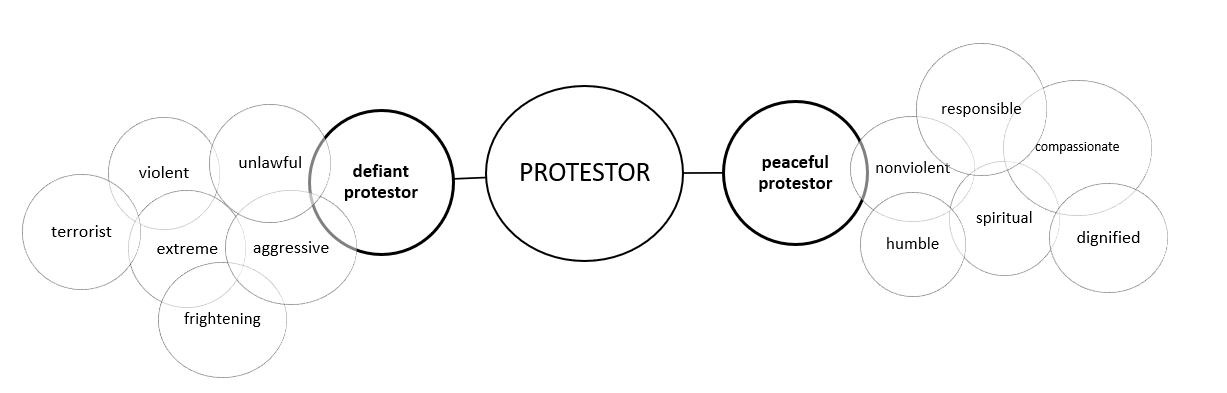
\includegraphics[width=14cm]{Figures/cluster.png}
\caption{Radial categories of \textsc{protester} with corresponding clusters of attributes}
\label{fig:figure1}
\end{figure}

\textbf{ICMs and Othering}

What is remarkable about the attributes in Table 4.2 and Figure 4.3, is the degree to which concepts on the opposing columns (or radial nodes) are opposites to each other. In short, the ICMs juxtapose. All Group A statements place protesters on the \textit{defiant protester} node, while all in Groups B and C place them on the \textit{peaceful} node. Moreover, the attributes on each side are not merely different variations, they are opposites. Here, we explore how this categorization is crucial to understanding the process of othering.

There is evidence to suggest dualistic thought patterns are hardwired into the human brain. According to \citeauthor{LeDoux1994}'s (\citeyear{LeDoux1994}) studies on the neurology of emotions, any information entering the central nervous system is unconsciously assigned a ``good'' or ``bad'' label \citep[31]{Wood2005}. Moreover, this choice is determined by the amygdala before further processing by the cortex.  At least when it comes to emotions and the unconscious, the tendency to categorize information in a dualistic manner seems deeply rooted in the human mind. However, the fact that information is unconsciously categorized by the amygdala does not imply there is no room for further cognitive processing. Further processing and modulating of sensory information is possible since ``the cerebral cortex can dialogue with the amygdala'' \citep[32]{Wood2005}. More sophisticated thinking that accounts for gradation and nuance depends precisely on this dialogue.   

Othering can be understood in terms of dualistic, emotional thought processes. At its essence, identifying another human as `other' is to create a polar dichotomy between that human and the `self'. As an unconscious, emotionally driven cognitive process, othering builds upon this polar diachotomy with what \citeauthor{Fedor2014a} (\citeyear{Fedor2014a}) calls ``antagonistic pairs.''        

\begin{quote}
The relation between me-the other one can be illustrated through a series of antagonistic pairs....similar-different; local-foreign; close-far; friend-enemy; normal-deviant; majority-minority. (322)   
\end{quote}

Considering the ICM used by Group A speakers to categorize \textsc{protester}, we can see antagonistic pairs being created through the discourse. Unlawful-lawful and orderly-disorderly are two examples. Local-foreign is also at play, as exemplified in the following statements:

\begin{footnotesize}
\begin{itemize}
\item[] \texttt{Unfortunately, a lot of times these things can be overwhelmed from outside groups.\newline 
\textit{-Senator Scott Martin}}
\newline
\item[] \texttt{There is an element there of people protesting who are frightening. It's time for them to go home. \newline 
\textit{-North Dakota Attorney General Wayne Stenehjem}}
\end{itemize}
\end{footnotesize} 

The portrayal of protesters as originating from outside the area is a discursive move that is consistent with the \textsc{protester} ICM. To describe the protesters as ``local'' or ``neighbours'' would be inconsistent with the other dichotomies that underpin the protesters as `other'. The phrase ``go home'' might be interpreted in a similar way. Or, one might consider another dichotomy as private-public, where ``home'' denotes the private sphere. This would expand the idea discussed in the socio-economic level, where Group A speakers present themselves as maintaining public order in the name of protecting the private sphere.

Othering manifests as stereotype when `in group' and `out group' dynamics come into play. `Self' and `other' takes on the dimension of `us' and `them'. Like the notion of the other, us/them identities are created through discourse. The preceding discussion gives examples of how ``out group'' status is assigned to protesters. In Group A, we can also see more subtle appeals to the in-group. For example, the repeated claim that protesters are a ``public safety issue'' creates an `in group' of law abiding citizens. Similarly, the claim that protesters ``make life difficult for everyone who lives and works in the area,'' is an `in group' of all local working people. Finally, when the Attorney General refers to a donation from the pipeline company Energy Transfer partners as ``a gift to the people of North Dakota,'' all people of the state are an `in group' vis-\`a-vis protesters who, despite also being citizens, have been cast as an `out group'.      

\textbf{Summary of the Cognitive Level}

By reading quotes from the corpus, one can quickly see that pipeline protesters are being portrayed using consistent language and concepts, particularly related to aggressive and unlawful behaviour. Not only do the various speakers in Group A refer to protesters in a consistent manner, but the language they use is often opposite to that of Groups B and C. While it is expected that Groups B and C would contrast with Group A, the extent to which pipeline proponents/opponents employ polar opposite concepts is noteworthy. 

The notion of Idealize Cognitive Models (ICM) is one way to understand how protesters are framed according to two opposing radial categories: \textit{defiant protester} and \textit{peaceful protester}. Attributes cluster around these radial nodes. The othering and stereotyping arises from this binary categorization of the concept \textsc{protester}. In other words, ICMs give us a framework for understanding the apparent stereotyping of protesters as a consequence of the way humans unconsciously categorize information.

\section{Summary \& Conclusions}

This chapter opened by highlighting the diverse perspectives surrounding infrastructure projects like the Dakota Access Pipeline (DAP). It was also pointed out that, due to the high profile nature of this project, the volume of communication is particularly large. If attempting to analyze the issue, the breadth of perspectives and communication artifacts presents a methodological challenge. In order to address this challenge, a multilevel approach using corpus data was employed. Specifically, quotations were extracted in order to break down the large volume of linguistic data into meaningful segments. Organizing the quotations into three groups (A, B, and C) made it possible to carry out a comparative analysis. The following is a summary of the analysis.

\begin{itemize}
  \item Keywords suggest dominant themes among proponents (Group A) to be security and law. Group A keywords also indicate possible negative portrayals of pipeline opponents. \textit{Protester} is the second most common keyword in this Group. Group B keywords also contain language related to public institutions and laws (e.g. \textit{right}, \textit{government}). Also, ecological-related terms appear in Group B (e.g. \textit{land}, \textit{water}). Group C has some overlap with B, but cultural terms are more apparent (e.g, \textit{sacred}, \textit{prayer}).
  
 \item In Group A, nature is referred to in the context of resources and management. Energy and infrastructure are discussed in terms of security and safety. An overarching discourse strategy in Group A is establishing and upholding legitimacy over resources and infrastructure. 
 
  \item In Group B, the natural environment is contested as a site of political/economic injustice. Power dynamics of resources and infrastructure are discussed. Group B can be seen as being in dialogue with Group A, insofar as an overarching discourse strategy is challenging the legitimacy of institutions to manage natural resources.
  
  \item In Group C, nature is a source of cultural identity. Statements refer to a holistic relationships between people, culture, and economy. Group C operates in an entirely different frame of meaning than both A and B. 
  
  \item In Group A, we notice that identifiable sub-groups of the population are not mentioned. Protesters and opponents are anonymized and disassociated from society. Group A statements suggest that othering involves a stripping away of culture.
  
  \item Clusters of concepts used in Group A show how othering and stereotyping might result from the way humans categorize information. The negative associations with pipeline opponents can be understood in terms of Idealized Cognitive Models (ICMs) of the concept \textsc{protester}.

\end{itemize}

One could make the case that the above results are merely consistent with the way in which groups were selected. For instance, one would expect Group A to portray protesters in a negative light, Group C would contain cultural keywords, and so on. However, the main conclusions from this analysis arise from the comparison of communication between the groups, not each group in isolation. By contrasting Groups A and B with Group C, we get clearer insight into what constitutes cultural discourse. 

In Chapter 2, we discussed the nuanced and fuzzy distinction between the cultural and socio-economic levels. The former was associated with \textit{Kultur} as an inner spirit of human experience; the latter with \textit{Zivilization} with the outer shell. In this light, one might consider Groups A and B as having to do with \textit{Zivilization}. The groups dealt with institutions, administrative systems, and corporate structures that encompass all a society. Group C, by contrast, was the source of identity and expression of inner (cultural) meanings within the society.     % Analysis 2

\chapter{Analysis 3: Nonverbal Communication in Mining Debates}
\lhead{\textit{Analysis 3: Nonverbal Communication in Mining Debates}}

\textit{\textbf{Chapter Summary:} This chapter uses a multimodal corpus to consider nonverbal communication in the context of mining debates. This level of analysis gives insight into cognition and emotions in ways that textual data does not. These insights have important implications for the framing of environmental issues.}
\newline

\section{Multimodal, Nonverbal Communication}

The analyses in preceding chapters focus on language as text and, in the case of Analysis 2, textual representations of verbal communication. Of course, text is just one of many possible modes of human communication. While many insights can be gained from textual discourse analysis, the nuances and richness of human culture come to the fore when communication is multimodal. Multimodal communication draws from the textual as well as aural, linguistic, spatial, and visual capacities or modes \citep{Murray2013}. From a corpus linguistic and discourse analysis standpoint, multimodal implies consideration of a wider range of media such as audio, video, and images. It also implies the consideration and analysis of a broad spectrum of integrated human communication including nonverbal behaviors and paralanguage.  

This third and final analysis considers communication as an integrated whole. Speech and text segment language into constituent parts such that meaning is constructed from the bottom up, from words to phrases, and so on. By contrast, in the \textit{Lebenswelt} of everyday communication, it is the combination of fluid verbal and nonverbal semiosis that creates meaning. Estimates of the degree to which human communication is nonverbal have varied. Depending on the context, it has been suggested that over 90 percent of communication is nonverbal \citep{Mehrabian1972}, but this figure depends highly on the context and is not a universal claim. Elsewhere, it has been suggested two-thirds of all communication is nonverbal \citep{Burgoon2016}. Regardless, of the exact estimates, it suffices to say that nonverbal communication is integral to overall meaning and understanding.

Nonverbal can refer to a wide range of information transfer through visual, auditory, tactile, and kinesthetic channels. For this present analysis, however, we focus particularly on gestures and facial expressions. Paralanguage, such as pitch and intonation, will also be considered secondarily. In addition, nonverbal communication is considered alongside speech rather than in isolation. The rationale for not isolating the nonverbal is that verbal statements provide necessary context to interpret the meaning of gestures and expressions. Each of the elements (gesture, facial expression, paralanguage, etc.) is a vast, specialized topic. The present aim, therefore, is a more general interpretation of holistic communicative acts.

\section{Corpus Data}

From a corpus linguistics and discourse analysis standpoint, multimodal implies the consideration and analysis of a broad spectrum of integrated human communication including nonverbal behaviors. More precisely, a multimodal corpus is defined by \cite*{Foster2008} as

\begin{quote}
an annotated collection of coordinated content on communication channels such as speech,
gaze, hand gesture, and body language, [that] is generally based on recorded
human behaviour (4).
\end{quote}

Thus, in addition to the data itself (i.e. recorded human behaviour), annotation of the multimodal corpus is a defining feature. However, annotation is a challenge for multimodal corpus research given both the time it requires as well as the lack of annotation standards \citep{Abuczki2013}.

For Corpus 3, the recorded human behaviour consists of audio and video representing different perspectives on mining and natural resource development. These include interviews, documentaries, recordings of `town hall' type meetings. The data was collected manually using a search engine (most results were from \textit{YouTube} and some from archives of news broadcasting agencies). Transcripts were then obtained for each media item and saved as separate files (\textit{txt} format).

There are 25 files in total, each with a url associated back to the original audio/visual media. The transcripts include timestamps (e.g. 05:45). By looping through the transcripts and getting the last timestamp, the total runtime of the media was calculated as 7 hours 46 minutes. The average runtime is about 18 minutes.

Rather than annotating the entire corpus, selections were obtained using both top-down and bottom-up approaches. In the top-down approach, the media was watched/listened to manually, paying close attention to gesture, body language, or other non-verbal expressions. Timestamps of interest (i.e. points in the recording with distinctive and pronounced non-verbal expression) were then marked for further annotation. The bottom-up approach began by searching for keywords and phrases related to analytical themes (i.e. ecology, culture, socio-economic). Segments related to key themes were then identified for further analysis and annotation. 

The next step was interpretation and analysis. There are competing theories concerning the meaning and interpretation of nonverbal communication (NVC). Topics of debate include the extent to which nonverbal behaviours are universal by virtue of our common biological or evolutionary origins, or the degree to which they are culturally variable \citep[e.g.][]{Jack2012}. Also debated is whether nonverbal behaviors are reflective of internal, cognitive states or whether they are better understood in terms of social interaction and influence \citep[e.g.][]{Crivelli2018}. These debates are touched upon in this chapter, but their details are generally beyond the current scope.

The present analysis aims, first and foremost, to be descriptive. Nonverbal analyses of this specific genre (i.e. environmental communication) are limited. Comparative data and observations are, therefore, valuable, even if interpretation is limited. The descriptive segments consist of video transcripts with annotations, together with footnote physical descriptions of nonverbals. The annotation method used is based on that of \cite{Jefferson2004}, as summarized in Table 5.1. Image frames from the video segments are also included.

Following each description is a brief interpretive narrative. The purpose of the narrative is to tie together the various NVC elements as well as integrate them with the verbal component. These narratives generally include some discussion, based on secondary literature, of what the nonverbals \textit{could} mean. Considering gestures, facial expressions, paralanguage, together with the verbal language, the following questions guide interpretation:

\begin{itemize}
\item What does the NVC tell us about the emotional state of the speaker?
\item How does the NVC complement, or contrast with, the verbal communication?
\item Does NVC give insight into how the speaker is thinking?
\end{itemize}

Following the descriptions and interpretations of each segment, comparison and analysis across all the segments is conducted.   

\begin{table}[H]
\begin{footnotesize}
\centering
\def\arraystretch{1.1}% 
\begin{tabular}{ | P{2cm} P{3cm} P{6cm}|}  
\hline
(.)             & Micro-pause                    & A brief pause, usually less than 0.2 seconds.                                                                      \\ \hline
. or down arrow & Period or Down Arrow           & Indicates falling pitch or intonation.                                                                             \\ \hline
? or up arrow   & Question Mark or Up Arrow      & Indicates rising pitch or intonation.                                                                              \\ \hline
,               & Comma                          & Indicates a temporary rise or fall in intonation.                                                                  \\ \hline
!-              & Hyphen                         & Indicates an abrupt halt or interruption in utterance.                                                             \\ \hline
>text<          & Greater than/Less than symbols & Indicates that the enclosed speech was delivered more rapidly than usual for the speaker.                          \\ \hline
<text>          & Less than/Greater than symbols & Indicates that the enclosed speech was delivered more slowly than usual for the speaker.                          \\ \hline
\degree         & Degree symbol                  & Indicates whisper, reduced volume or quiet speech.                                                                 \\ \hline
ALL CAPS        & Capitalized text               & Indicates shouted or increased-volume speech                                                                       \\ \hline
underline       & Underlined text                & Indicates the speaker is emphasising or stressing the speech.                                                      \\ \hline
:::             & Colon(s)                       & Indicates prolongation of a sound.                                                                                 \\ \hline
hhh             &                                & Audible exhalation                                                                                                 \\ \hline
.hhh            &                                & Audible inhalation                                                                                                 \\ \hline
(text)          & Parentheses                    & Speech which is unclear or in doubt in the transcript.                                                             \\ \hline
[text]          & Square brackets                & Speech within square brackets is accompanied by the meaningful part of the gesture - the so-called `stroke phase'. \\ \hline
\end{tabular}
\caption{Gail Jefferson's (\citeyear{Jefferson2004}) annotation scheme as adapted by \cite[5]{Beattie2016}}
\label{tab:table1}
\end{footnotesize}
\end{table}

\section{Multilevel Analysis}

Compared to the corpora covered in the previous two chapters, there are a number of considerations in light of a multimodal corpus. The first difference concerns the blending of topics. In previous chapters, the levels of analysis are segmented (ecological, cultural, socio-economic, cognitive). Textual corpora allow for this segmentation as the topics of discourse could be discerned at the sentence level. This separation continues in this chapter, but the multimodal corpus highlights the extent to which the levels blend in the normal flow of verbal communication. In the text corpora, there are often definitive boundaries between themes. By contrast, in this corpus it is common to find a combination of cultural, socio-economic, and ecological themes within a single phrase. This makes segmentation of levels more difficult than it was in Analyses 1 and 2. 

There are also differences in the language itself. Since data from the multimodal corpus consist entirely of spoken/conversational language, differences from the other (textual) corpora can be expected. While the extent to which there are sharp differences between written and spoken English is debatable \citep{Biber1988}, one might expect a spoken language corpus to include shorter, simpler sentences, less lexical diversity, less nomialization (usage of nouns versus verbs), and high contextualization.   

A keyword analysis of the corpus transcripts points to some of these language differences. Recall that in both Analyses 1 and 2, keywords were indicative of overall themes and often contained rich, specialized lexical items. In the present corpus, the top ten keywords are: \textit{know}, \textit{people}, \textit{right}, \textit{mining}, \textit{think}, \textit{one}, \textit{like}, \textit{mine}, \textit{say}, \textit{going}, and \textit{year}. With the possible exception of \textit{mining} and \textit{mine} these keywords are very generic and hardly indicate overall discourse themes. These results are indicative of the highly contextual nature of spoken language. The contextual nature of the multimodal data means that, in analysis and interpretation, less emphasis can be placed on lexical items. Consider that the previous two analyses began by looking at lexical items. Keywords and concordance lines were used to isolate points of interest in the data. These points of interest were then examined in more detail to infer patterns of meaning in the communication. While, this present analysis will also draw on lexical items (from transcripts), it does not rely on text to the same degree. 

Rather than lexical items, points of interest are identified from segments which contain particularly expressive nonverbal communication. The aim of selecting segments from the multimodal data is to identity moments where speech and nonverbal expressions combine to underscore meaning. These moments are what \cite*{McNeill2005b} calls points of ``highest communicative dynamism'' (1). 

In the present analysis, we examine multimodal communication through source data consisting of about 8 hours of video segments. From the 8 hours of video, 13 clips were selected for annotation and detailed analysis. Although the segments are diverse in length and genre, they share a common theme; namely, mining development. The segments include interviews, round table discussions, town hall meetings, etc. on the topics of deep sea mining, uranium mining, mountain top coal mining, mineral extraction and economic development, and other related themes. 

The analysis that follows presents 4-6 examples for three of the levels: ecological, cultural, and socio-economic. Rather than presenting separate examples from the cognitive-level, the cognitive analysis will go deeper into the segments presented in the first three levels.

\subsection{Ecological Level}

For the ecological level, excerpts were selected wherein speakers are explicitly discussing ecological issues. These excerpts are not based on keywords and concordances (as in the previous analyses), but were selected manually, from a qualitative survey of the data. Despite the nearly 8 hours of video on the topic of natural resource development, there are relatively few cases where the speech segments clearly fell into the ecological level, meaning there are not coinciding political, cultural, economic themes within the excerpts.

Below there are four examples of ecological-level communication. Three of these excerpts feature subject matter experts who employ technical and scientific concepts. The final example features a citizen protester. Example 1 below consists of an excerpt and accompanying gestures in Figure 5.1. In this segment, a researcher is discussing impacts of deep sea mining.

\textbf{\underline{Ecological Level - Example 1}}

\begin{footnotesize}

\texttt{(the) [\annotate{direct} impact]\textsuperscript{1} will likely result in biodiversity loss that will be very difficult to [recover from,]\textsuperscript{2} but we \annotate{really} don't understand is any of the [\annotate{wider} impacts]\textsuperscript{3} as well, so outside the [area of]\textsuperscript{4} mining itself <how will this> [affect the ecosystem at large how will this feedback into the oceans]\textsuperscript{5} we think that the deep sea...}

\end{footnotesize}

\begin{footnotesize}
\begin{enumerate}
   \item Hand downward in swift movement, fingers pointed outward
   \item Hands in cycling motion forward
   \item Hands expanding outwards
   \item Hand in wide circular movement with palm down
   \item Hands in cycling movement with palms inwards
\end{enumerate}
\end{footnotesize}

\begin{figure}[H]
\centering
\begin{tabular}{llll}
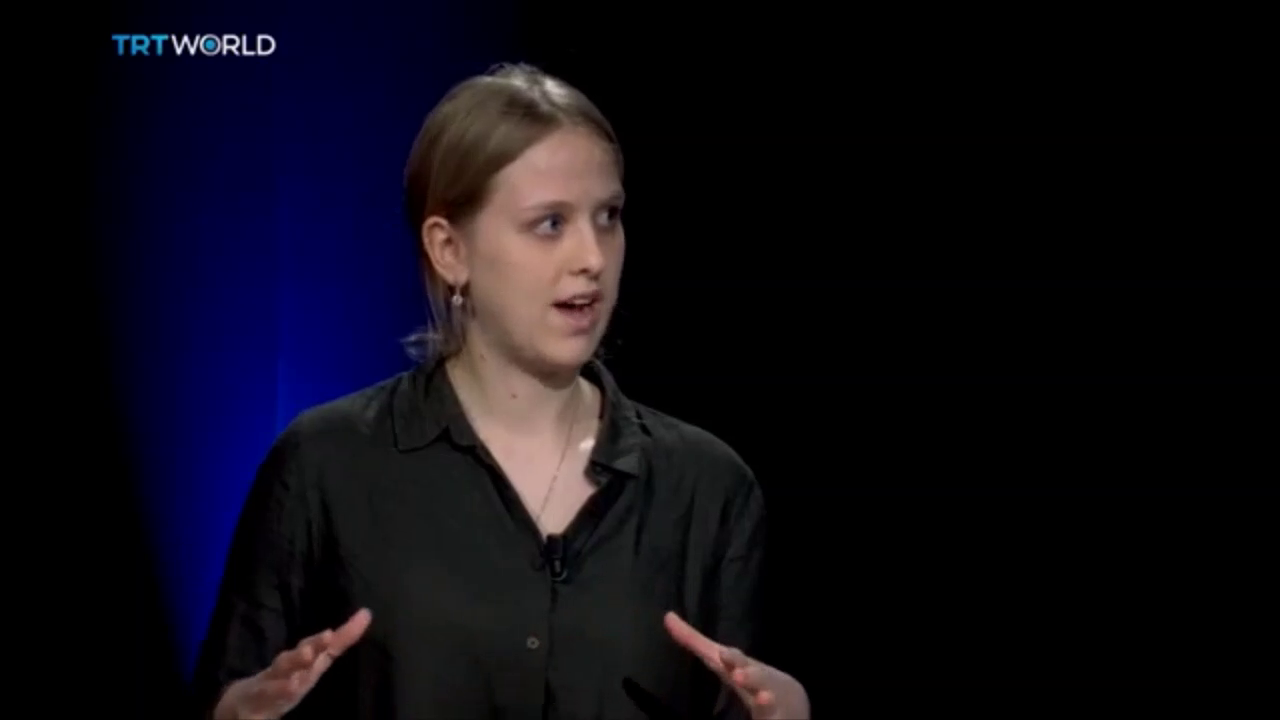
\includegraphics[width=4.2cm]{Figures/mmEco/frame207.png} & 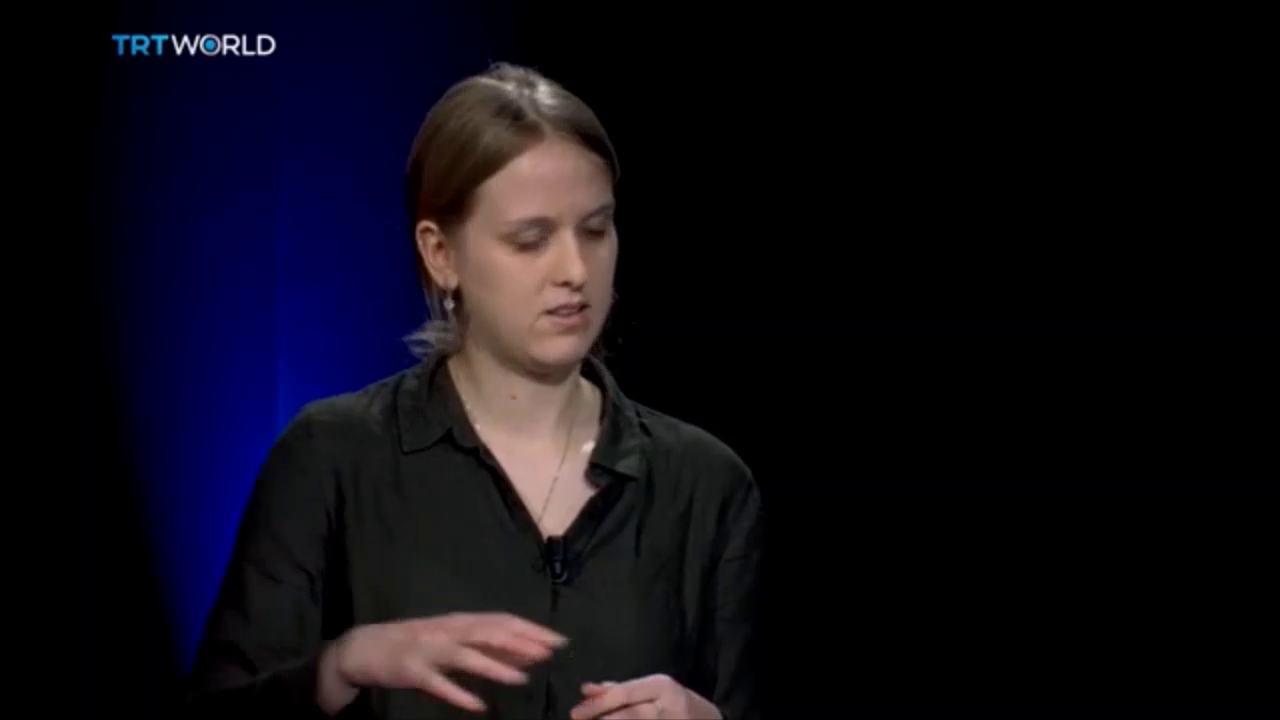
\includegraphics[width=4.2cm]{Figures/mmEco/frame252.png} & 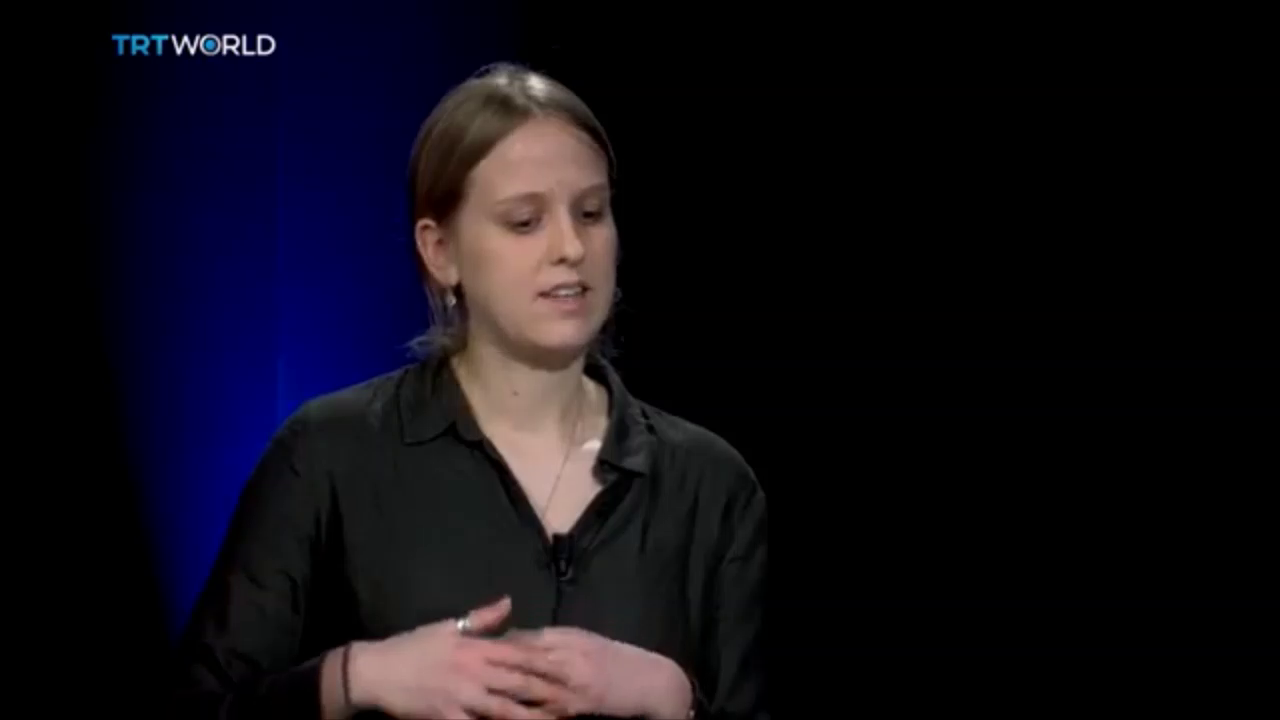
\includegraphics[width=4.2cm]{Figures/mmEco/frame392.png} 

\end{tabular}
\caption{Ecological Level - Example 1}
\begin{footnotesize}
Left: hands open palms down gesture with fingers extended to emphasize direct ecological impacts. Middle, Right: Hands loosened, palms inward/down in a cycling motion to reflect less certain long term ecological processes and feedback mechanisms.\\

Source: \url{https://www.youtube.com/embed/-UPjsuuyvD4?start=632&end=653}
\end{footnotesize}
\label{fig:figure1}

\end{figure}

Noticeable in Example 1 are the controlled hand gestures. The hands reflect the physical and ecological processes taking place. For instance, ``direct impact'' of mining is accompanied by a swift downward movement or arms and hands. The fingers and thumbs extended with palms facing downward are indicative of impact and gravity in a short time frame. When speaking of the ``area of mining'' the palm is similarly facing downward with a circular motion of the hand, indicating surety of the impacts in the mining area. By contrast, the cycling motions of the hands indicate a longer time frame of ``feedback'' and wider impacts. The palms shift to face inwards with more relaxed (non extended) fingers and thumbs, suggesting less certainty about these long term impacts. So, in this excerpt we see how the direction of palms and extension of fingers/thumbs reflect degrees of certainty and uncertainty.

Beyond hand gestures, other nonverbals are noticeable. For much of the segment the head is tilted to the side, which has been interpreted as a sign of interest, curiosity, and uncertainty \citep[94]{Lewis2012}. There are moments where the eye gaze shifts upwards which, in  European/North American cultures is commonly seen as a sign that someone is thinking \citep{McCarthy2006}. Finally, it should be noted that facial expressions in Example 1 are minimal and do not convey any apparent emotions. 

Example 2 features a researcher talking about concerns associated with coal mining near a nature reserve. 

\textbf{\underline{Ecological Level - Example 2}}

\begin{footnotesize}
\texttt{Where our [concern lies is with respect to \annotate{dust}!- because there's no analysis of the dust(.) in terms of the toxic components in that dust]\textsuperscript{1} given the coal mining and the blasting and that sort of thing\degree. Now, you can feel [\annotate{this wind}. <This wind>]\textsuperscript{2} (.) is blowing across us [right into the game reserve]\textsuperscript{3}, so [if] they mine here, this south-easterly wind will carry the dust and the fallout will be in the park, >in the wilderness area<.}   
\end{footnotesize}

\begin{footnotesize}
\begin{enumerate}
   \item Hand in front facing inwards palms open thumbs up
   \item Hands pointing left hand to left
   \item Hand (right) pointing to the right
\end{enumerate}
\end{footnotesize}

\begin{figure}[H]
\centering
\begin{tabular}{llll}

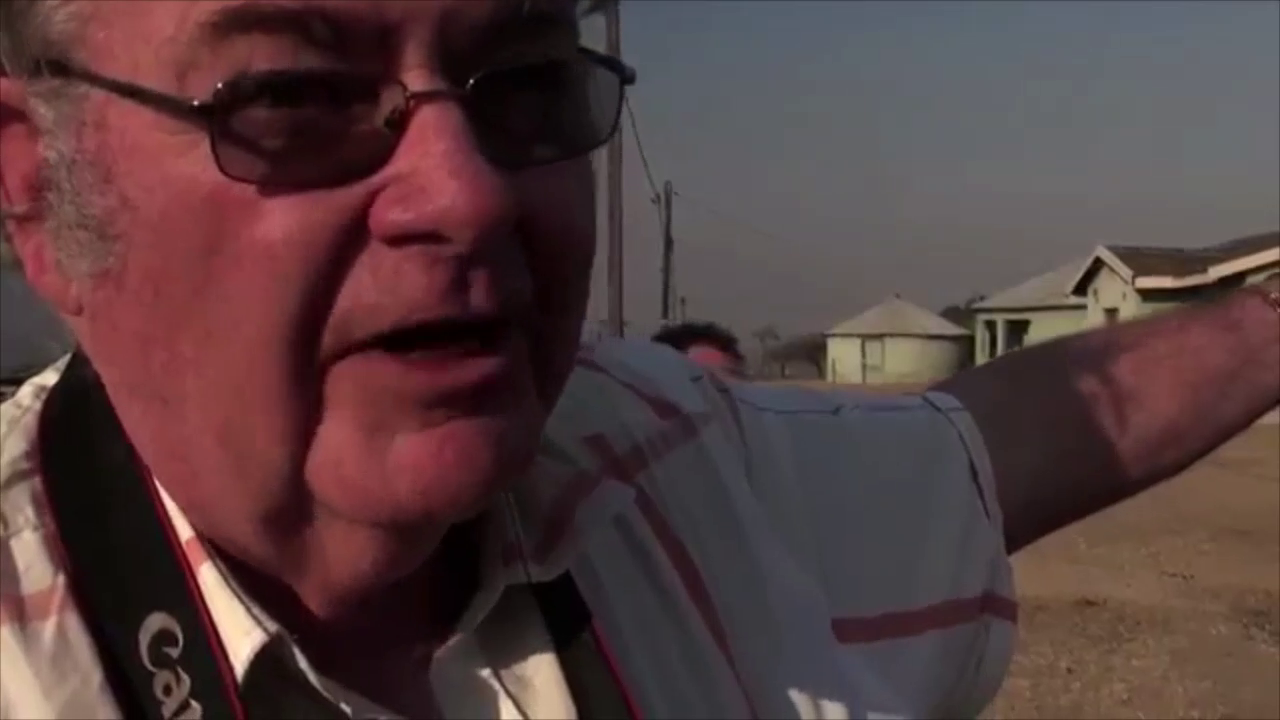
\includegraphics[width=4.2cm]{Figures/mmEco1/frame578.png} & 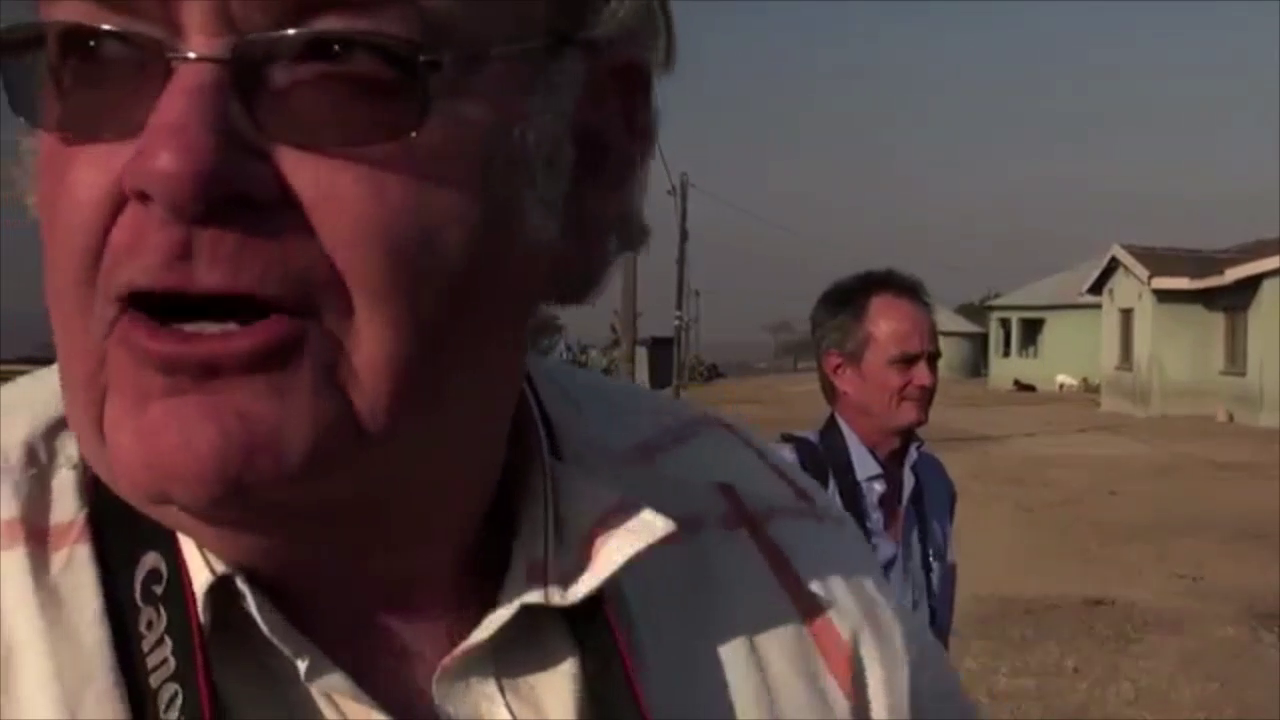
\includegraphics[width=4.2cm]{Figures/mmEco1/frame619.png} & 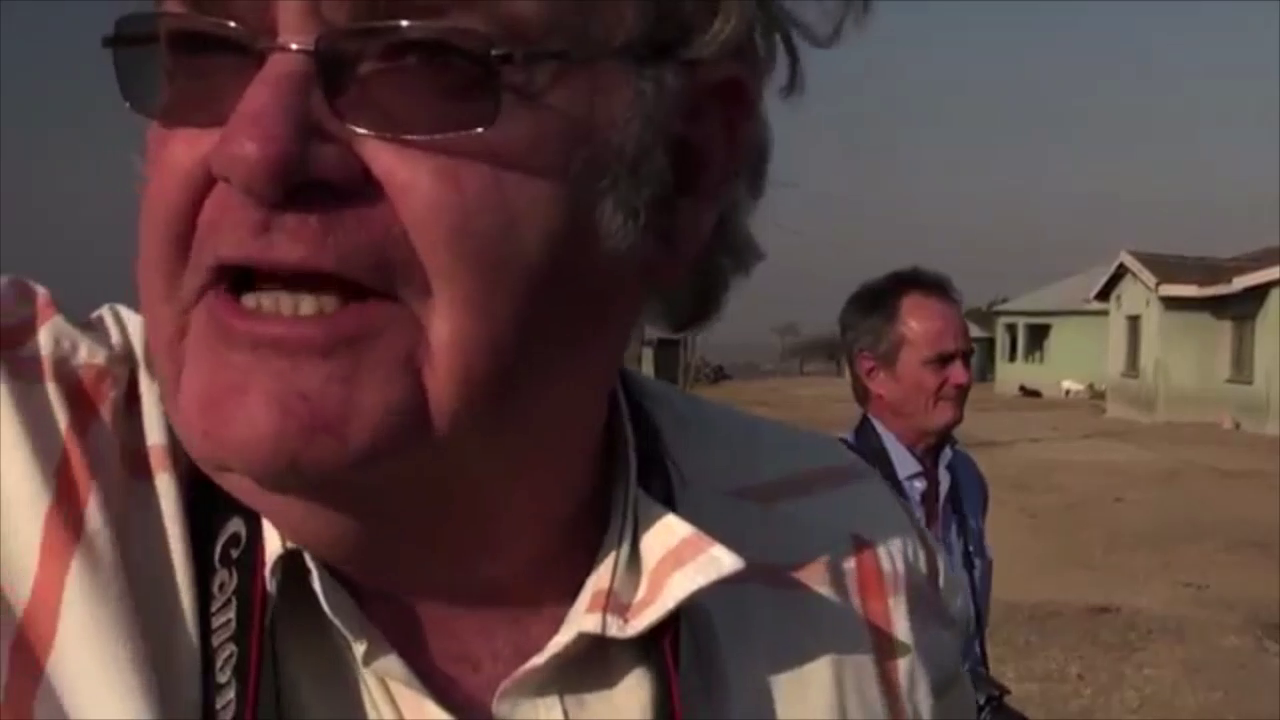
\includegraphics[width=4.2cm]{Figures/mmEco1/frame634.png}  

\end{tabular}
\caption{Ecological Level - Example 2}
\begin{footnotesize}
Hand and arm points to left (Left image) and then to right (Right image) to reflect the physical movement of dust.\\

Source: \url{https://www.youtube.com/embed/Sh0_Wf8F4RM?start=857&end=888)}
\end{footnotesize}
\label{fig:figure1}
\end{figure}

Though difficult to see in the frame, when the man in Example 2 is speaking about ``our concern,'' the palms are inward. The fingers and thumbs are extended and the hands motioning up and down with speech emphasis. This cluster of hand gestures suggests possession (palms inward to express \textit{our} concern)  as well as a confidence that this is serious (thumbs up) perhaps with a degree of uncertainty (palms inward). Also, as in the previous excerpt, the hands and arms are used to describe physical and ecological processes which, in this case, is the directional transfer of dust.  

Compared with Example 1, there are several indicators in Example 2 suggesting the speaker's emotions are at play. In the first excerpt, hand movements are used to complement and reiterate the verbal communication. On the second, however, the nonverbals give more of an indication about what is not explicit verbally. For instance, the furrowed eyebrows indicate stress and concern, as do stress lines on the forehead. The swift, agitated up and down movement of hands also convey a sense of urgency. The speaker places stress on certain words (e.g. ``dust'', ``wind'') and changes the speed and cadence.    

In Example 3, an engineer or industry representative is facing questioning on contamination of groundwater due to coal mining. 

\textbf{\underline{Ecological Level - Example 3}}

\begin{footnotesize}
\texttt{People don't understand that <you have to> >[maintain a well just like you do your \annotate{car}]<.\textsuperscript{1} A lot of people just [turn on the spigot,]\textsuperscript{2} and they think [it's going to work for them]\textsuperscript{3} (.) when they have <things like iron hydroxide precipitate> (.) and other metals built up in [their wells (and) every time I go out on a well complaint, I tell people]\textsuperscript{4} you [need to have a friend at the local (.) volunteer fire department come out and flush your well (out)]\textsuperscript{5}....}  
\end{footnotesize}

\begin{footnotesize}
\begin{enumerate}
   \item Index finger and thumb together in precision
   \item Turning of index finger and thumb 
   \item Hand out palm up 
   \item Hand out palm up 
   \item Nodding
\end{enumerate}
\end{footnotesize}

\begin{figure}[H]
\centering
\begin{tabular}{llll}

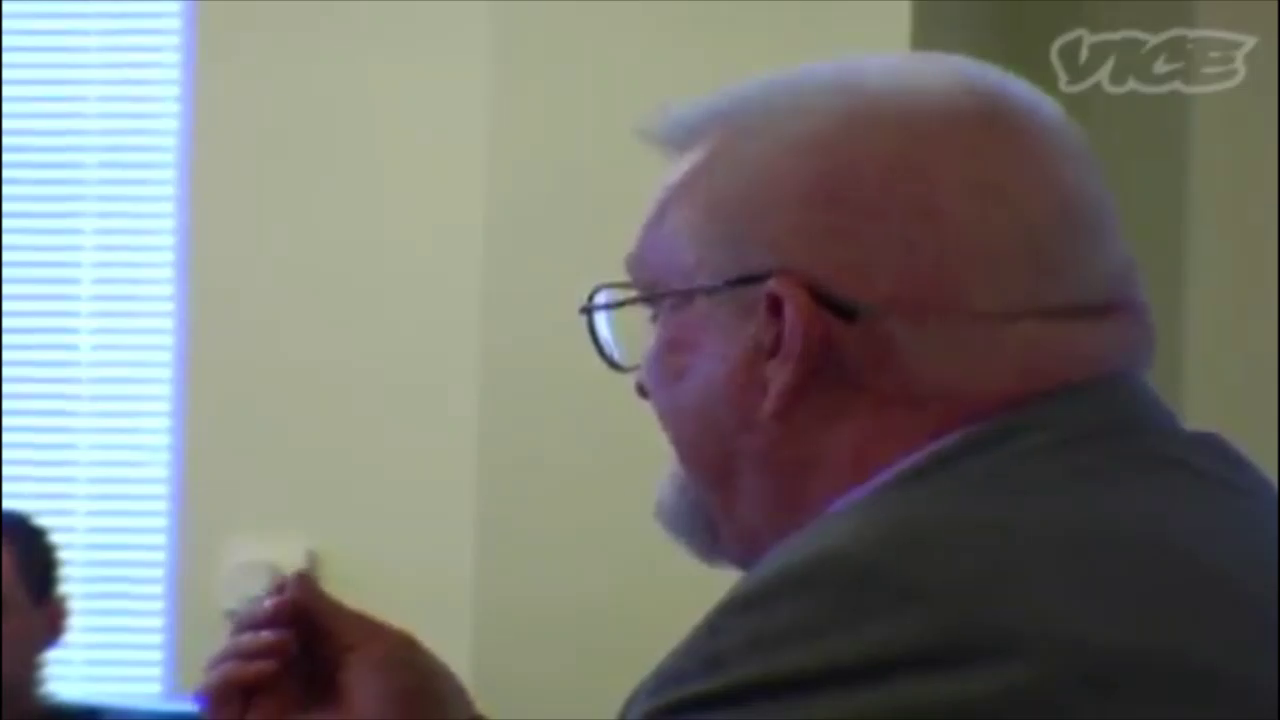
\includegraphics[width=4.2cm]{Figures/mmEco2/frame182.png} & 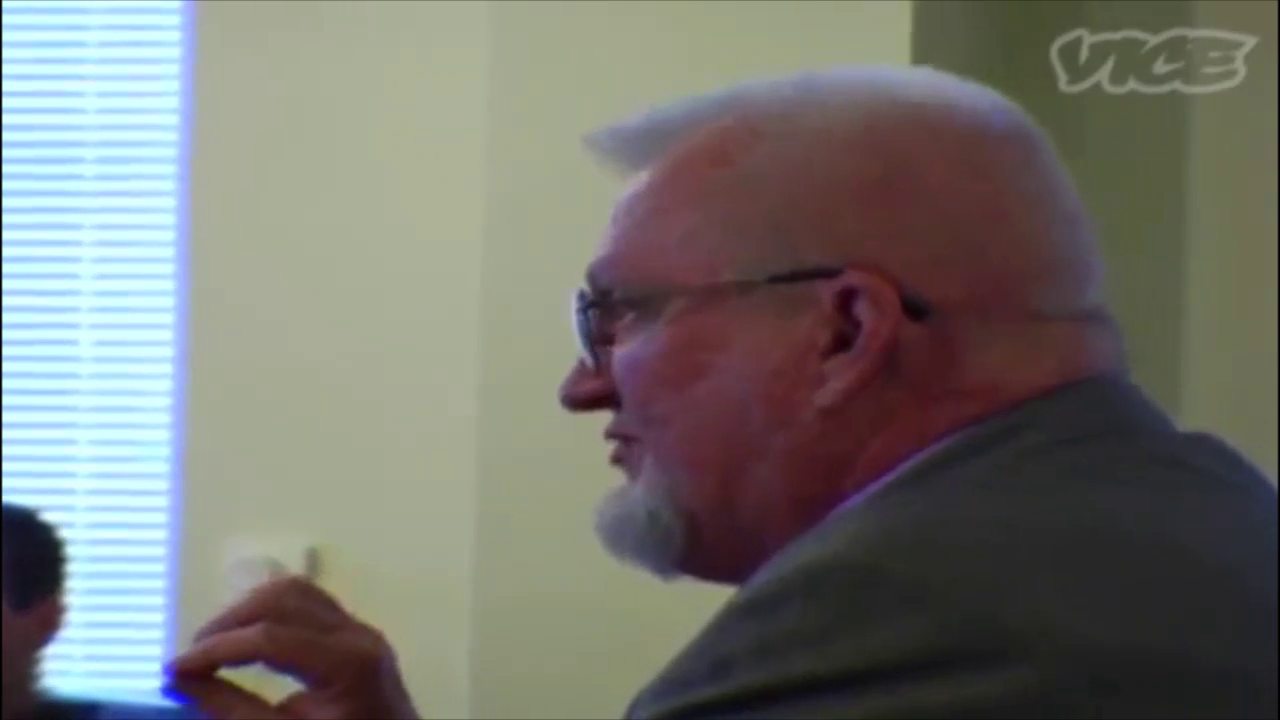
\includegraphics[width=4.2cm]{Figures/mmEco2/frame207.png} & 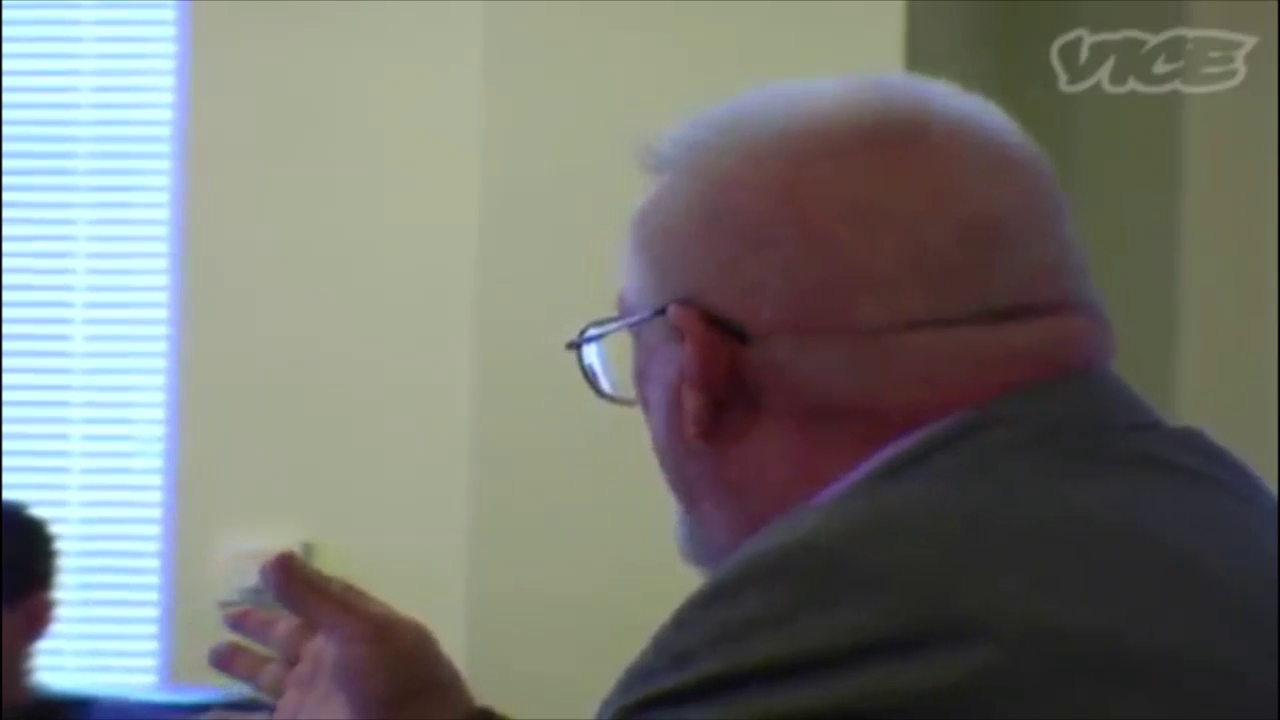
\includegraphics[width=4.2cm]{Figures/mmEco2/frame286.png}  

\end{tabular}
\caption{Ecological Level - Example 3}
\begin{footnotesize}
Left and Middle: the index finger and thumb join to create a precision movement. Right: the open hand palm up gesture functions as a suppliant offer of an idea.\\
Source: \url{https://www.youtube.com/embed/UvKe2LYy5pk?start=920&end=945}
\end{footnotesize}
\label{fig:figure1}
\end{figure}

In the context of the segment, the speaker is on the defensive, since he is trying to convince listeners that the coal industry is not responsible for water quality issues. A noticeable gesture is the touching of the thumb and index finger, which is accompanied by a turning motion when describing well operation. Like in the previous examples, hand gestures complement and emphasize the verbal communication by mimicking physical processes. Touching the index finger and thumb is also used in Western cultures to emphasize a point. The ring shape has been described by \cite{Kendon2004} and others as indicating precision. A possible effect of this gesture here is to focus and narrow the discussion to one of specific technical expertise.

In later frames, the speaker extends the right hand out with fingers extended and the palm rotated upward. The palm up is used for a variety of nuanced meanings including uncertainty, emphasis, emotional helplessness, and social deference \citep{GivensDavidB2016}. \cite{Muller2004} suggests that the function of the open hand palm up gesture is to present an idea for consideration. Here, the gesture functions as a non-forceful convincing plea. Given the context, one could interpret the palm up gesture as a rhetorical device, intended to convince and influence listeners. Other nonverbals might be interpreted in this way, as rhetorical, including the slight smile in early frames as well as a nodding at the end of the segment. The smile, it has been argued, is a way to appear nonthreatening to others \citep{Cunningham2004}. Nodding can be seen as a way to build rapport and activate mirroring between the speaker and listeners.

Example 4 is unique because of the constrained position of the speaker. This segment was filmed after protesters had been arrested and placed in hand restraints (Figure 5.4, Left). 

\textbf{\underline{Ecological Level - Example 4}}

\begin{footnotesize}
\texttt{[We've got to build a whole new energy infrastructure for this country, and if we don't we're going to have (.) climate chaos and our kids are going to \annotate{not} thank us for that].\textsuperscript{1}}
\end{footnotesize}

\begin{footnotesize}
\begin{enumerate}
   \item Continuous shaking of HEAD
\end{enumerate}
\end{footnotesize}

\begin{figure}[H]
\centering
\begin{tabular}{llll}

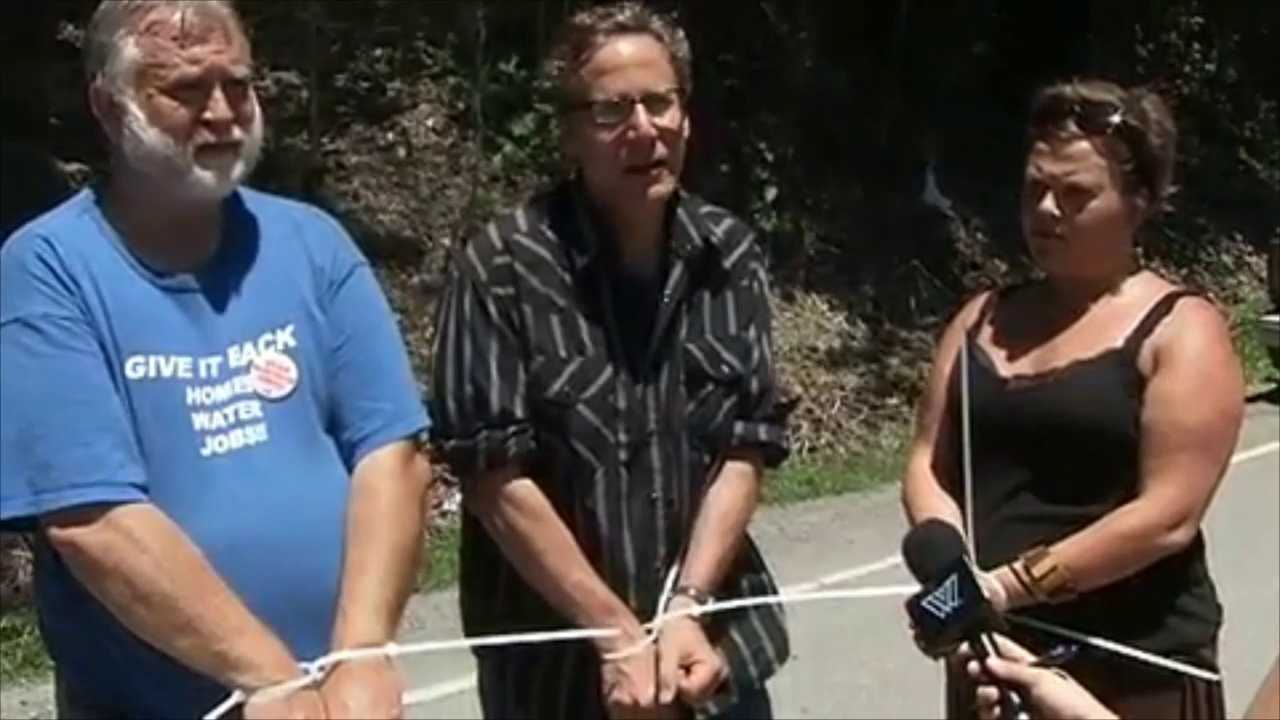
\includegraphics[width=4.2cm]{Figures/mmEco4/frame8.png} & 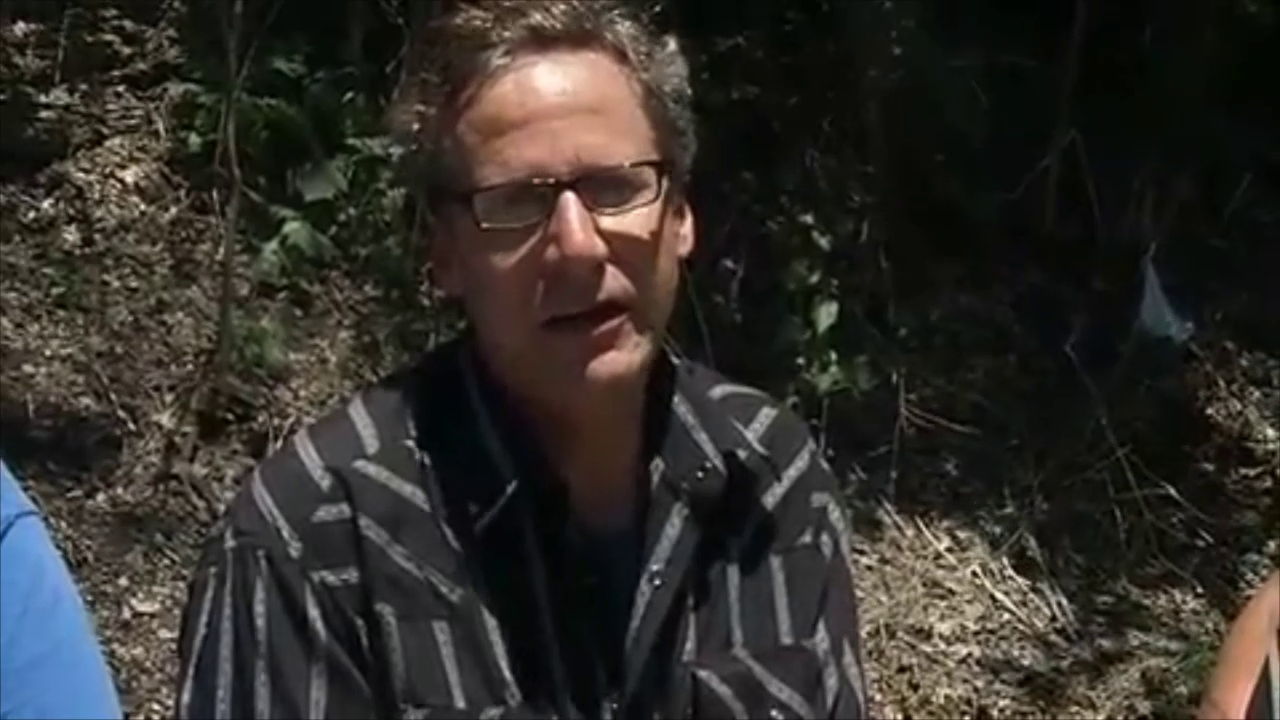
\includegraphics[width=4.2cm]{Figures/mmEco4/frame192.png} & 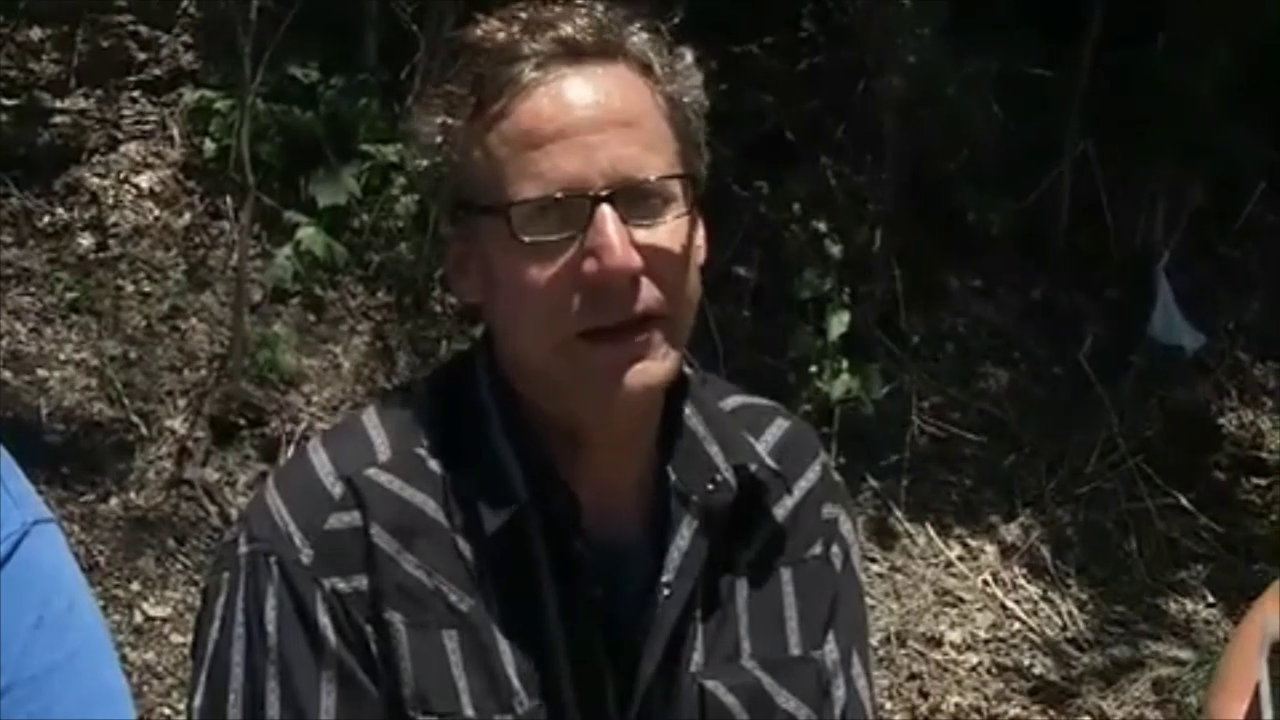
\includegraphics[width=4.2cm]{Figures/mmEco4/frame219.png}  

\end{tabular}
\caption{Ecological Level - Example 4}
\begin{footnotesize}
Left: hands constrained, possible accentuating communicative head movements. Middle, Right: continuous movement (shaking) of head from left to right carrying the meaning of unbelievable.\\
Source: \url{https://www.youtube.com/embed/vBhvFWRLiOs?start=821&end=829}
\end{footnotesize}
\label{fig:figure1}
\end{figure}

With the hands immobilized, gestures in Example 4 are confined largely to the head. In this segment, the speaker is expressing the need to build new energy infrastructure in the face of climate change. The words are accompanied by continuous shaking of the head. This head gesture might be interpreted as disapproval and condemnation. However, it can also be considered that this head shaking functions as a verbal intensifier with the negation carrying the meaning of ``unbelievable'' \citep[861]{McClave2000}. Also noticeable in this clip is the slight head tilt (also seen in Example 1). The facial expression might be interpreted as serious and sombre, but does not display a high degree of emotion.

\textbf{Summary of Ecological-Level}

The four examples above feature speakers from different points of view with respect to the ecological issues at hand. Of the four speakers, two are researchers, one is a company representative, and another is a protester. In all cases, the level of emotion expressed through nonverbal communication is minimal. While the second speaker does appear to convey some agitation or urgency through facial expressions and paralanguage, the overall segment is more a rational argumentation than an emotional expression. The last speaker, despite the context of being arrested, comes across as sombre and earnest, but not particularly emotional.

In the first three examples, gestures are predominantly iconic speech illustrators, meaning they display a close relationship with the content of the speech \cite[60]{Beattie2016}; \cite[76]{Matsumoto2012}. For instance, the first speaker uses deliberate and measured hand movements that reflect biophysical processes (ecological impact, recovery) expressed in speech. Also in Example 2, hand gestures reflect physical processes of dust transfer. The third speaker uses nonverbal hand movements to reflect the process of inspecting a well, but also employs what could be described as rhetorical gestures to convince listeners. 

\subsection{Cultural Level}

Examples in the cultural-level feature people expressing their cultural identities in some way. These identities take on different forms including national, sub-national/regional, ethnic, and religious. In Example 1, national cultural identity is being discussed in the context of resource development and cultural preservation in Afghanistan. Examples 2 and 3, invoke indigenous ancestry. In the case of Example 4, religion and spirituality come into play. Finally, in Example 5 we see an expression of local/regional identity.

The first example below is from a report on cultural heritage and extractive mining in Afghanistan. The segment is an interview with an Archaeologist who, based on his use of the phrase ``our identity,'' clearly identifies with Afghan culture.

\textbf{\underline{Cultural Level - Example 1}}

\begin{footnotesize}
\texttt{...with [all these wars (over) 30, 40 years]\textsuperscript{1}, (.) what the Afghan has lost we lost [our identity]\textsuperscript{2}!- and [I \annotate{believe}]\textsuperscript{3} to give (them) \annotate{back} that identity is only through [\annotate{culture}]\textsuperscript{4} !- because when it [\annotate{comes}]\textsuperscript{5} to culture, all Afghans are united.}
\end{footnotesize}

\begin{footnotesize}
\begin{enumerate}
   \item Left hand forward palm up; lateral sweep of head and hand
   \item Right hand motion to side; index finger extended; eyebrows raise
   \item Right hand motion to side; index finger extended; head tilts to one side
   \item Right hand motion forward; index finger extended
   \item Right hand motion forward; index finger extended; intonation on ``comes''
\end{enumerate}
\end{footnotesize}

\begin{figure}[H]
\centering
\begin{tabular}{llll}
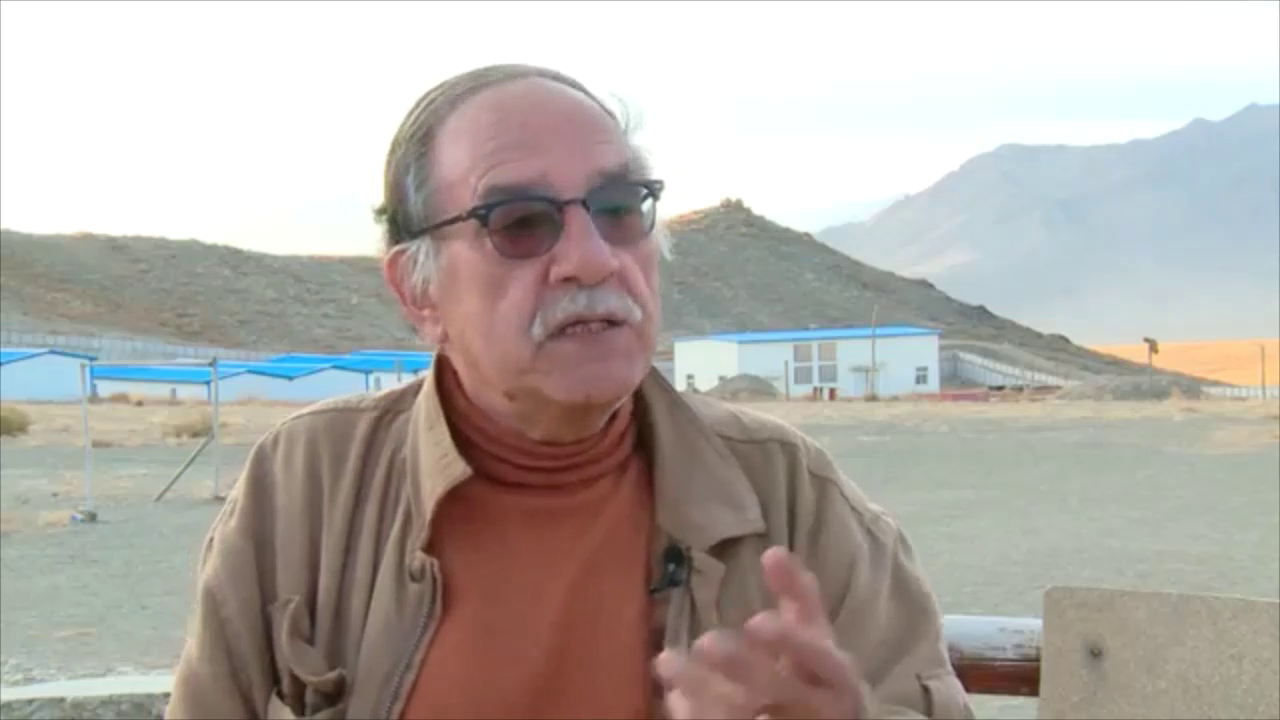
\includegraphics[width=4.2cm]{Figures/mmCult1/frame15.png} & 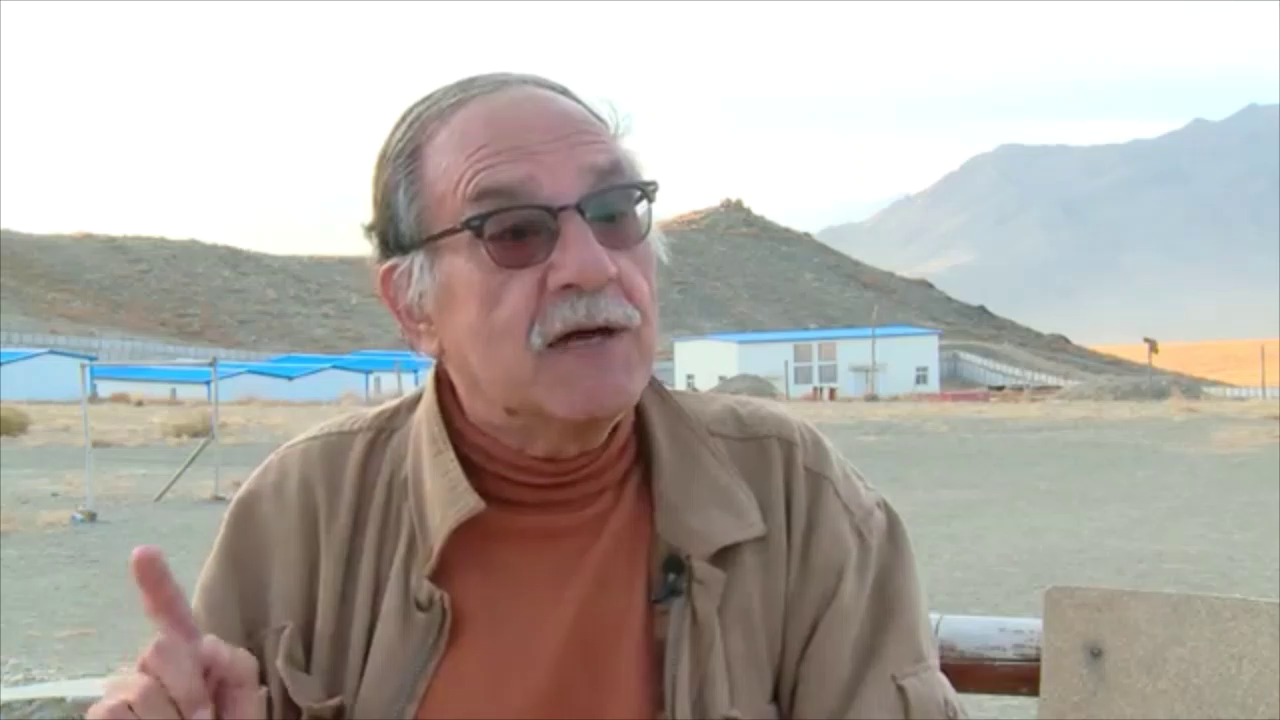
\includegraphics[width=4.2cm]{Figures/mmCult1/frame241.png} & 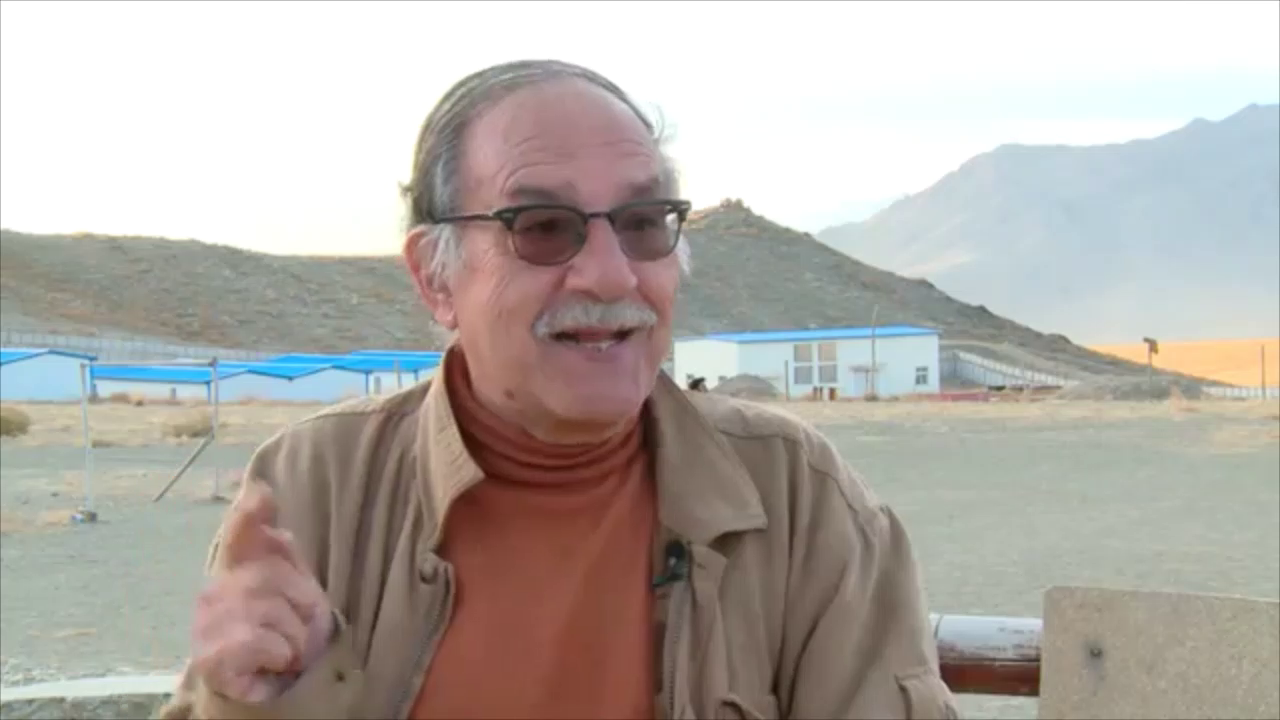
\includegraphics[width=4.2cm]{Figures/mmCult1/frame513.png} 

\end{tabular}
\caption{Cultural level - Example 1}
\begin{footnotesize}
Source: \url{https://www.youtube.com/embed/z6ewpjWYfYo?start=535&end=555}
\end{footnotesize}
\label{fig:figure1}
\end{figure}

The pointing of the finger in the above example functions to accentuate the message. There is a transition from palm up hand open (coinciding with ``with all these wars...''), to hand closed and index finger extended. This gesture transition coincides with emphasis in speech tone. Intonation and pauses with the words ``identity,'' ``culture,'' and ``comes'' further add emphasis. The pointing can also be an indication of high confidence in the message. In the previous ecological level excerpts, we mainly observe examples of iconic gestures that closely reflect the literal meaning of the speech. Here, we begin to see more metaphoric gestures that depict abstract ideas \citep[66]{Beattie2016}. For example, the sweeping motion to describe decades of wars is a metaphoric evocation of the passage of time. The pointing might also be interpreted as a metaphoric reference. Whereas pointing is typically a gesture used for object individuation \citep[115]{Kendon2003}, in this example it is used to `point to' the main concept in the message; namely culture and identity.      

In the next example, the video frame does not include hand gestures. However, there are subtle head movements and facial expressions. In this segment, the speaker is addressing the issue of a proposed mine near ancient burial sites. 

\textbf{\underline{Cultural Level - Example 2}}

\begin{footnotesize}
\texttt{(It's) [my prehistoric ancestors]\textsuperscript{1} (.) that are right within this mining area and [I don't want (.) .hhh hhh you know]\textsuperscript{2} [any \annotate{mine}]\textsuperscript{3} near them, >I don't want any equipment near them.< We have <three known \annotate{burial}> (mound) groups that are there.} 
\end{footnotesize}

\begin{footnotesize}
\begin{enumerate}
    \item Nodding head on beat
   \item Shaking head
   \item Left lip tightened and raised; slight raising of shoulders
\end{enumerate}
\end{footnotesize}

\begin{figure}[H]
\centering
\begin{tabular}{llll}
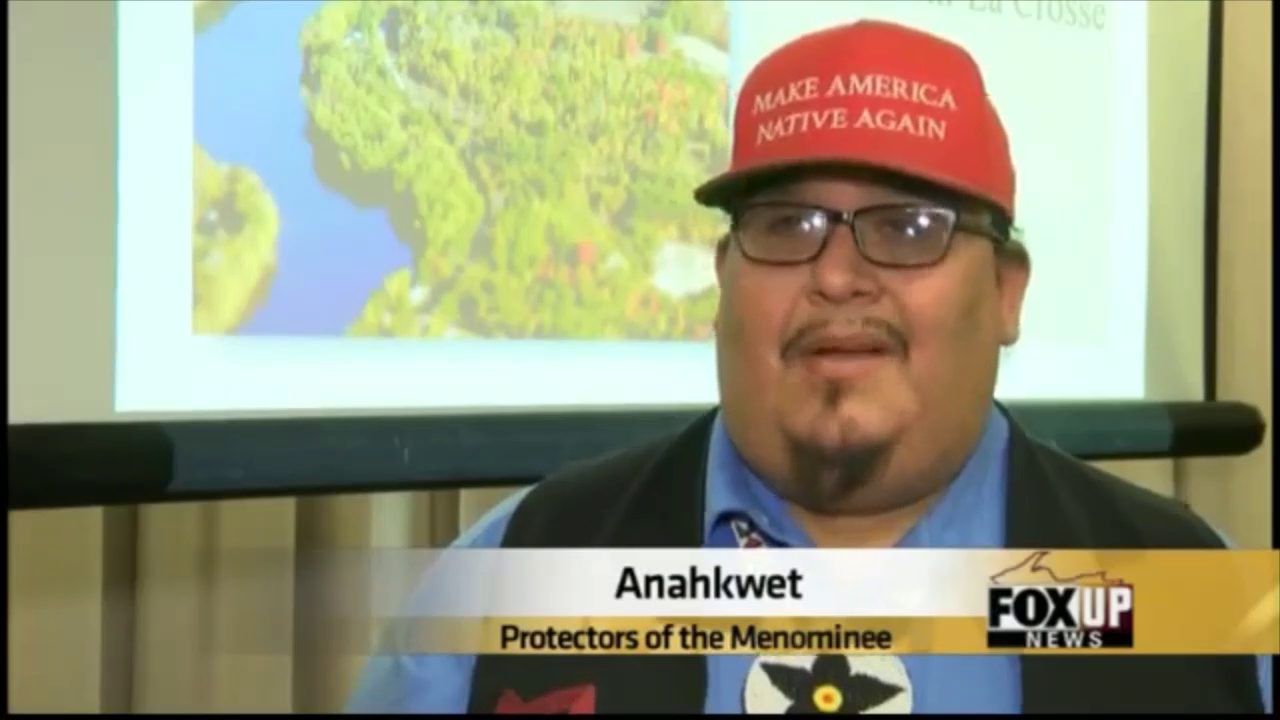
\includegraphics[width=4.2cm]{Figures/mmCult2/frame202.png} & 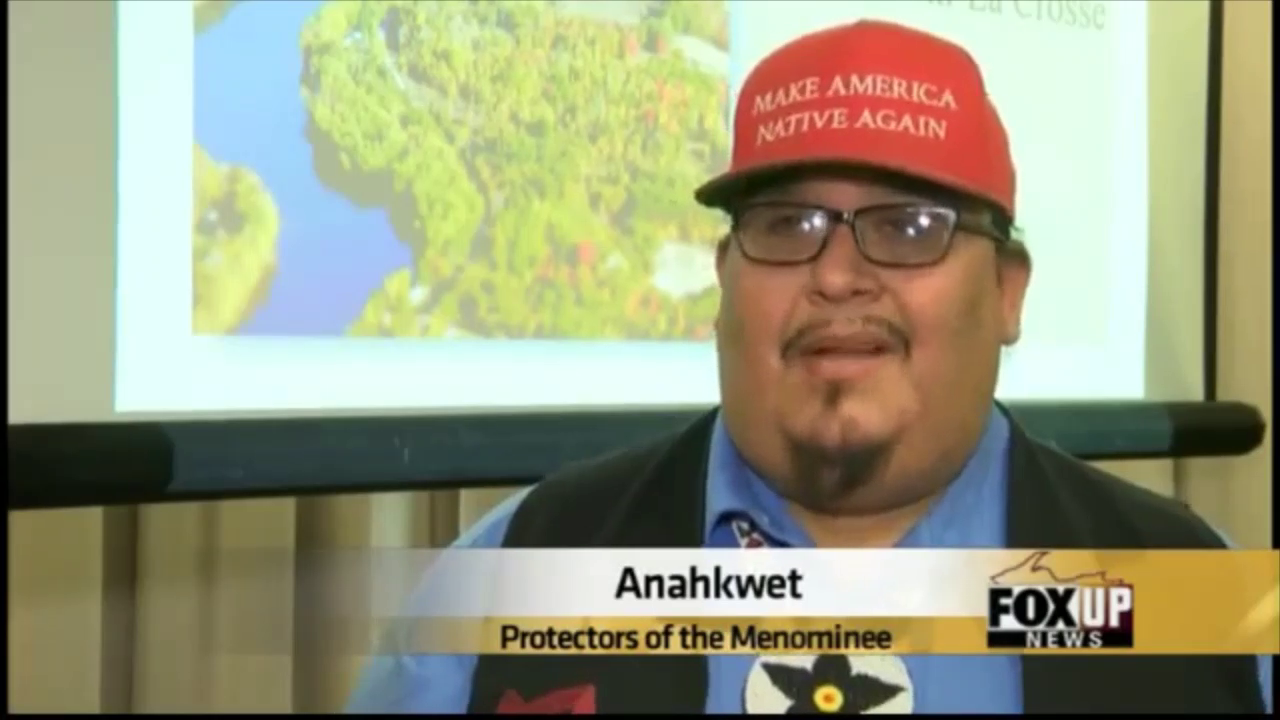
\includegraphics[width=4.2cm]{Figures/mmCult2/frame203.png} & 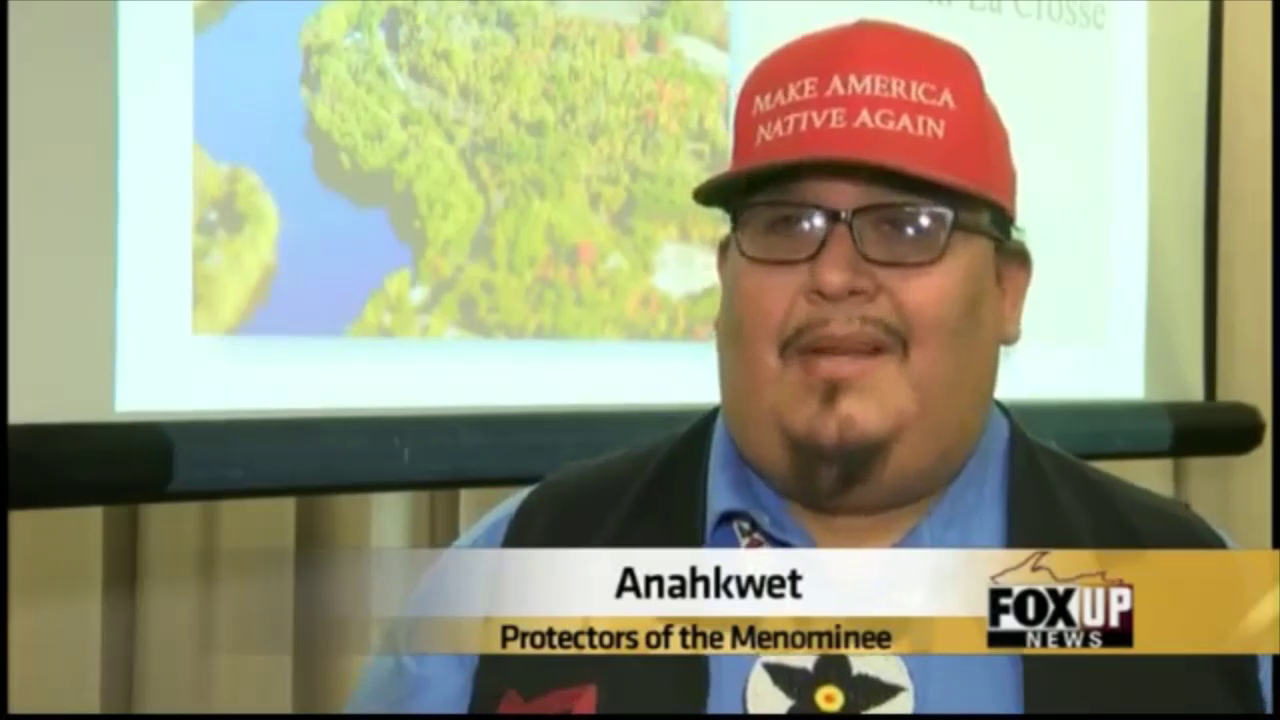
\includegraphics[width=4.2cm]{Figures/mmCult2/frame204.png} 

\end{tabular}
\caption{Cultural level - Example 2}
\begin{footnotesize}
Source: \url{https://www.youtube.com/embed/10FrfEa0Xck?start=33&end=45}
\end{footnotesize}
\label{fig:figure1}
\end{figure}

The head movements of nodding and shaking express emphasis and disapproval, respectively. The brief facial expression near the words ``any mine'' carries a high degree of emotional information. At this point, the corner of the lip is tightened and slightly raised. This expression is the topic of some of the earliest studies of body language. It is what \cite*{Darwin1872} described as ``the upper lip being retracted in such a manner that the canine tooth on one side of the face alone is shown'' (249-250). This was seen by Darwin as an expression inherent to both human and non-human animals when facing an antagonist. Sometimes referred to as a ``sneer,'' it's been suggested that this expression is a universal (cross-cultural) sign of contempt \citep{Izard1988}.

Elements of paralanguage are also observed in this segment. Stress is placed on the words \textit{mine} and \textit{burial}. There is also an audible inhale/exhale immediately before the contempt expression discussed above.  Altered breathing patterns can be indicative of agitation and emotional strain, including the anticipating of anger \citep[118]{Poyatos2002a}.

Example 3 below also relates to mining development on sacred indigenous grounds. Here, the hands, head, and eyes combine to form a cluster of nonverbals depicting the emotional context.

\textbf{\underline{Cultural Level - Example 3}}

\begin{footnotesize}
\texttt{<[They crushed out sacred site]>.\textsuperscript{1} They never [listened to aboriginal people, <elders, female elders>]\textsuperscript{2} (.) you know they've been [\annotate{stomped} on].\textsuperscript{3} So it's time for them to \annotate{stand} up and say [hey you're not doing this to me anymore].\textsuperscript{4}} 
\end{footnotesize}

\begin{footnotesize}
\begin{enumerate}
   \item Right hand motion forward on beat; palm up; index finger and thumb touching
   \item Right hand motion forward on beat; palm up; fingers and thumb open; high blink rate
   \item Head swipe, left to right with emphasis
   \item Head motion with clenched fist
\end{enumerate}
\end{footnotesize}

\begin{figure}[H]
\centering
\begin{tabular}{llll}

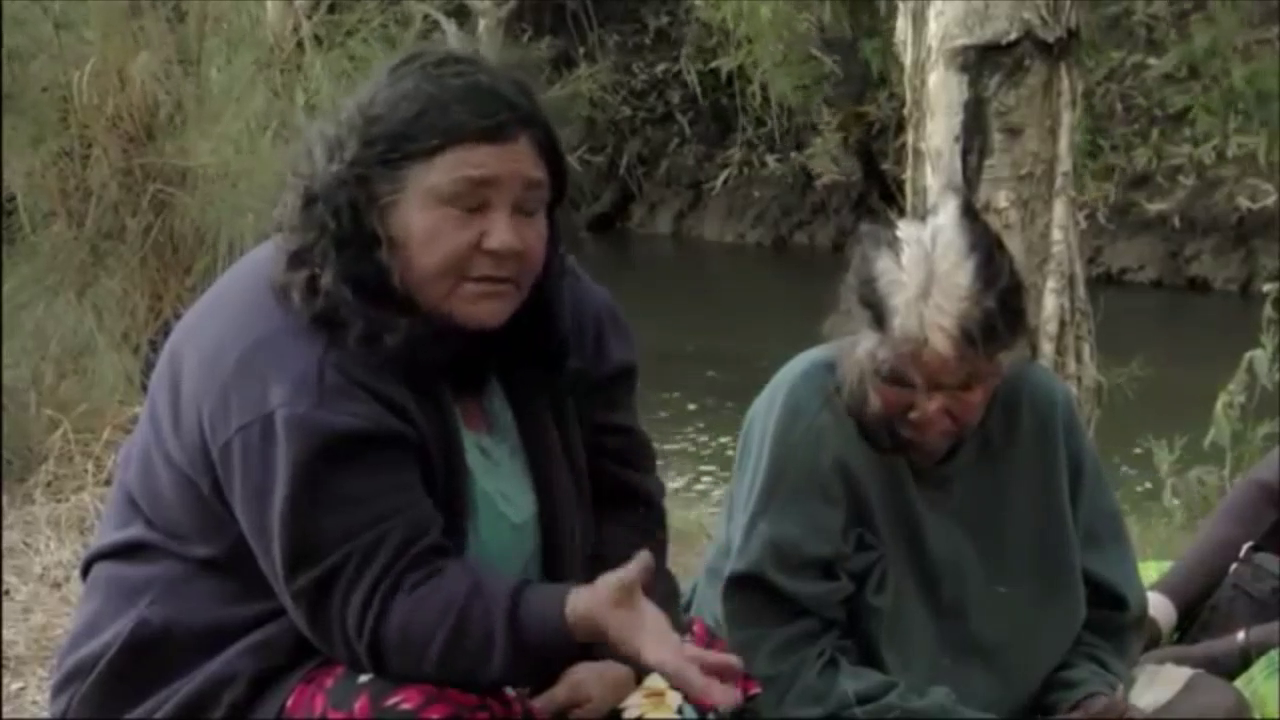
\includegraphics[width=4.2cm]{Figures/mmCult3/frame85.png} & 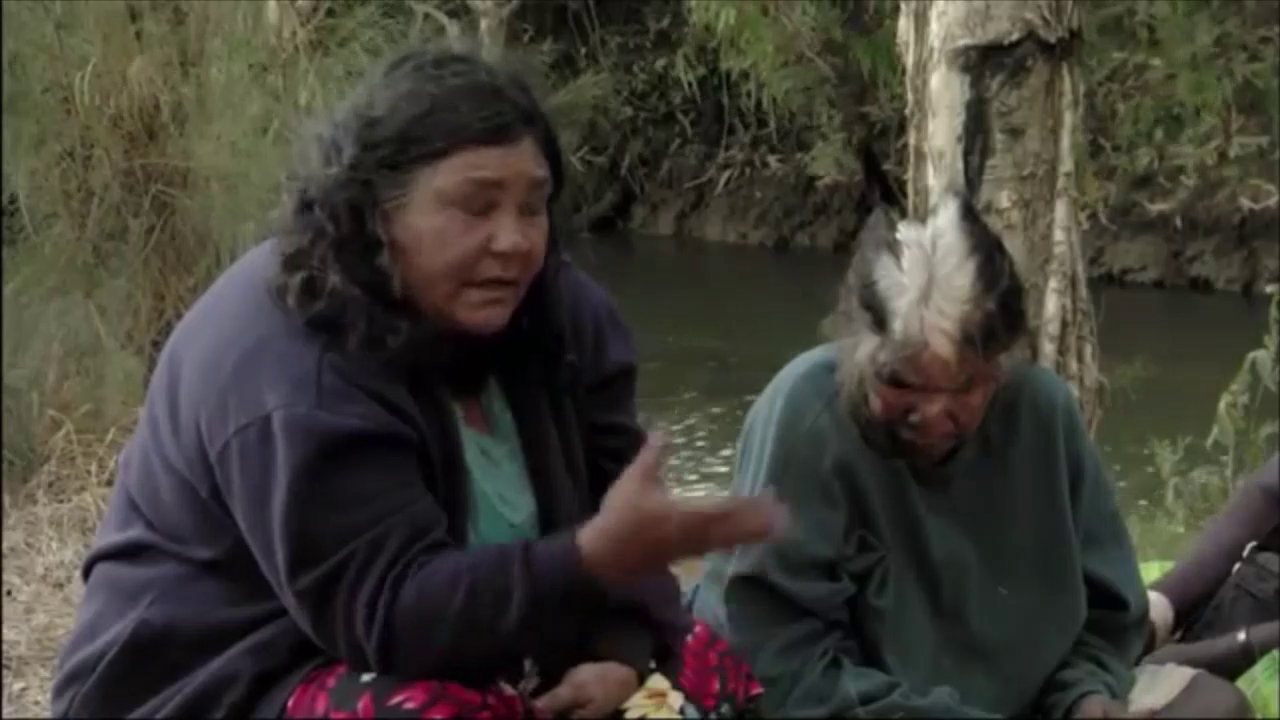
\includegraphics[width=4.2cm]{Figures/mmCult3/frame128.png} & 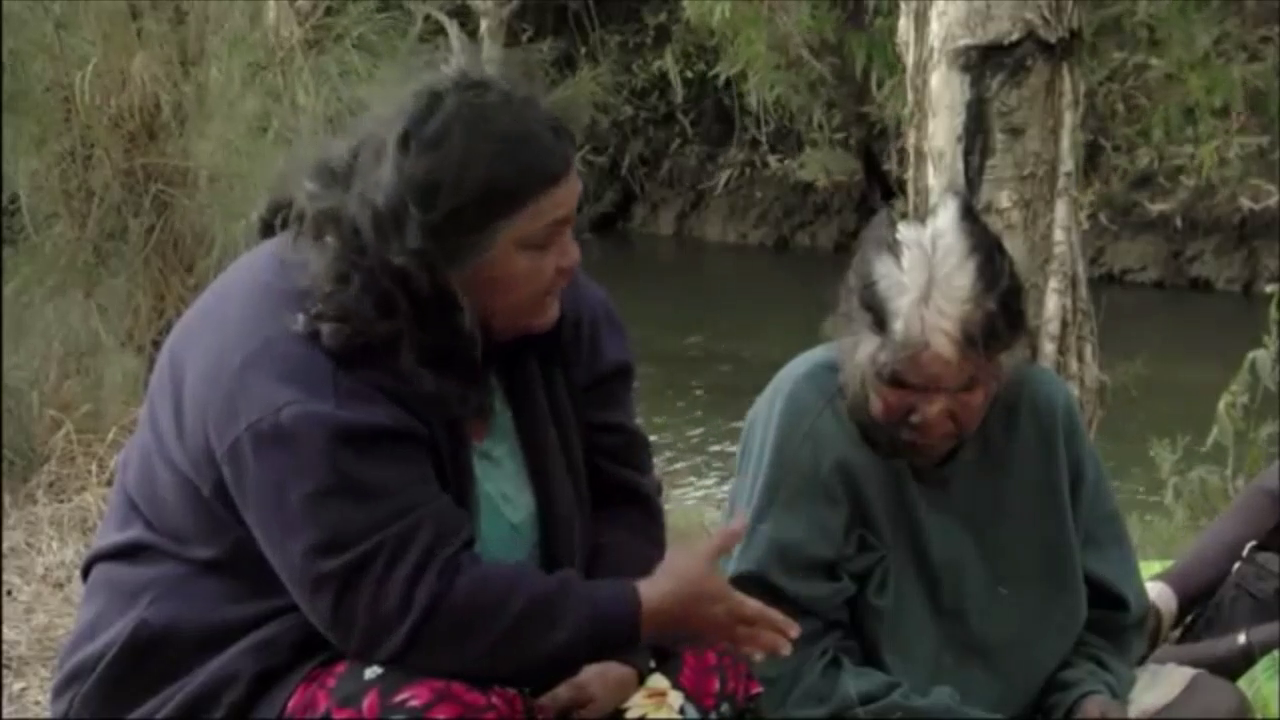
\includegraphics[width=4.2cm]{Figures/mmCult3/frame141.png}  

\end{tabular}
\caption{Cultural Level - Example 3}
\begin{footnotesize}
Source: \url{https://www.youtube.com/embed/awnLI4pRnUM?start=42&end=58}
\end{footnotesize}
\label{fig:figure1}
\end{figure}

As in previous examples, the on-beat hand movements are emphatic. The speaker clenches her fist when saying the words ``hey you're not doing this to me anymore.'' A clenched fist can be a sign of frustration, annoyance, or stress \citep[104]{Phipps2012}. It can also be interpreted as an ``encouragement gesture'' used communicate success or to function in self-encouragement or the encouragement of others \citep{Tops2006}. Here, the fist gesture could function as both an expression of frustration and affirmation to fight back. 

Also notable in Example 3 are the eyes and facial expressions. Around the words ``elders...female elders'' we observe a relatively high blink frequency and duration.  High blink rate (or lower blink inhibition) has been correlated to negative emotional states including stress \citep{Haak2019} and fear \citep{Maffei2019}. The speaker also displays narrowed eyes and a furrowed forehead, both strong indicators of negative emotions.

The context of the next excerpt, Example 4, is drinking water contamination due to mountain top coal mining. This is included in the cultural-level due to the religious sentiments expressed. As in the previous example, both hand and eye movements are telling indicators of emotions. 

\textbf{\underline{Cultural Level - Example 4}}

\begin{footnotesize}
\texttt{You \annotate{pray} before you go to bed... and >you just ask God to protect (you and) your family, that's all you \annotate{can} do,< because (.) [\annotate{man} has done the damage to the earth (.) and man]\textsuperscript{1} (.) [I don't see how <man can correct what's been done>]\textsuperscript{2}. [\annotate{God} can handle this (.) and he will. When the right time comes]\textsuperscript{3}, he will do what needs to be done.}
\end{footnotesize}

\begin{footnotesize}
\begin{enumerate}
   \item Right hand motions forward; palm up
   \item Right hand motions forward, fingers and thumbs curled inward; head shaking
   \item Rand waves outwards, stops at thigh; gaze upwards to sky; nodding 
\end{enumerate}
\end{footnotesize}

\begin{figure}[H]
\centering
\begin{tabular}{llll}

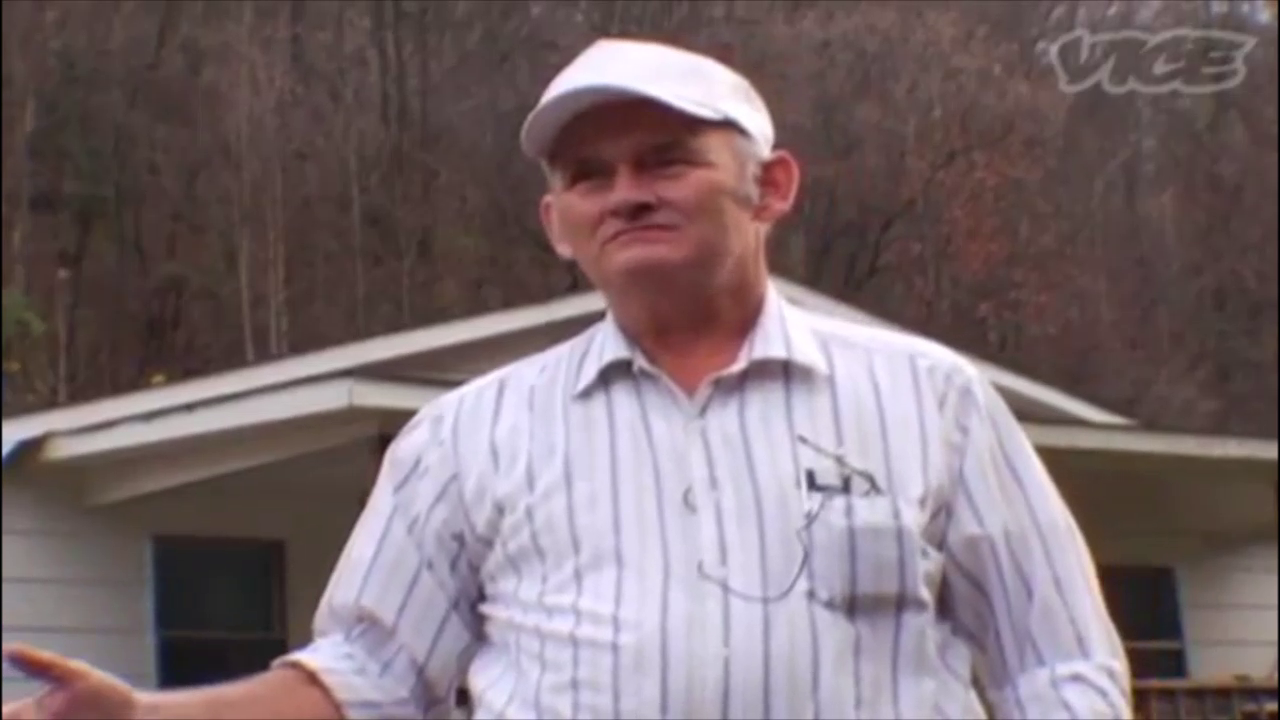
\includegraphics[width=4.2cm]{Figures/mmCult4/frame237.png} & 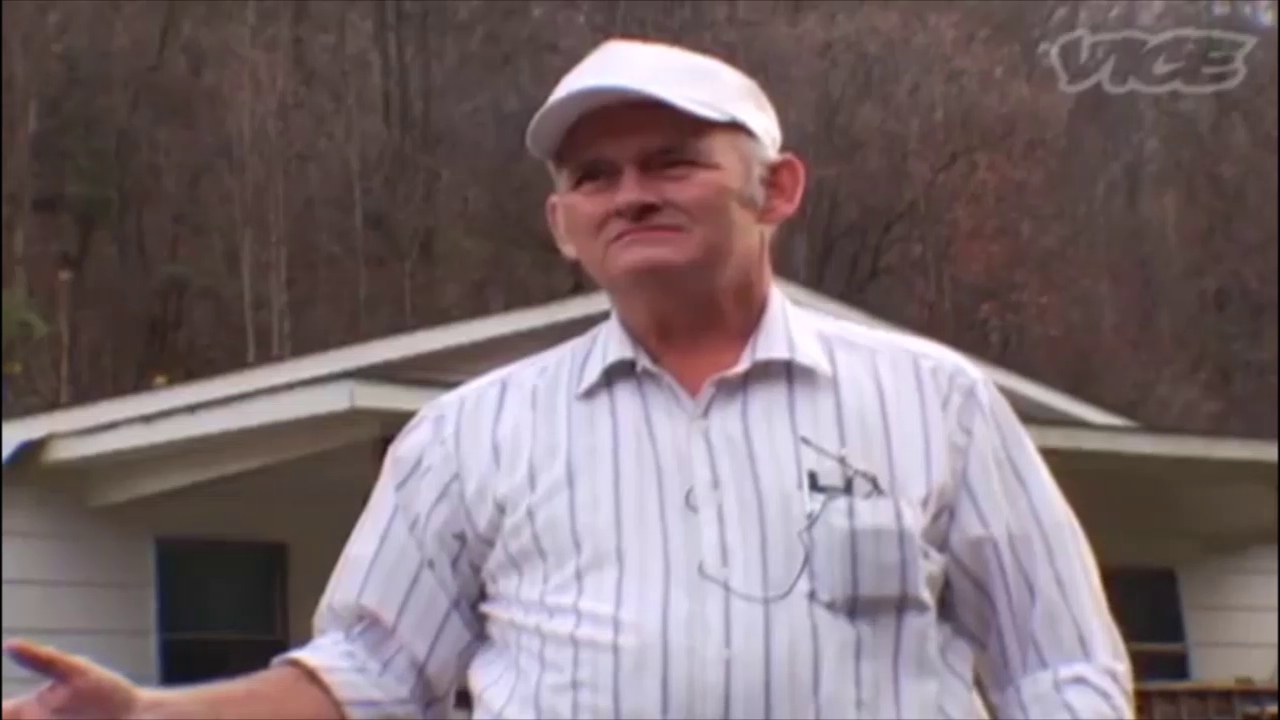
\includegraphics[width=4.2cm]{Figures/mmCult4/frame245.png} & 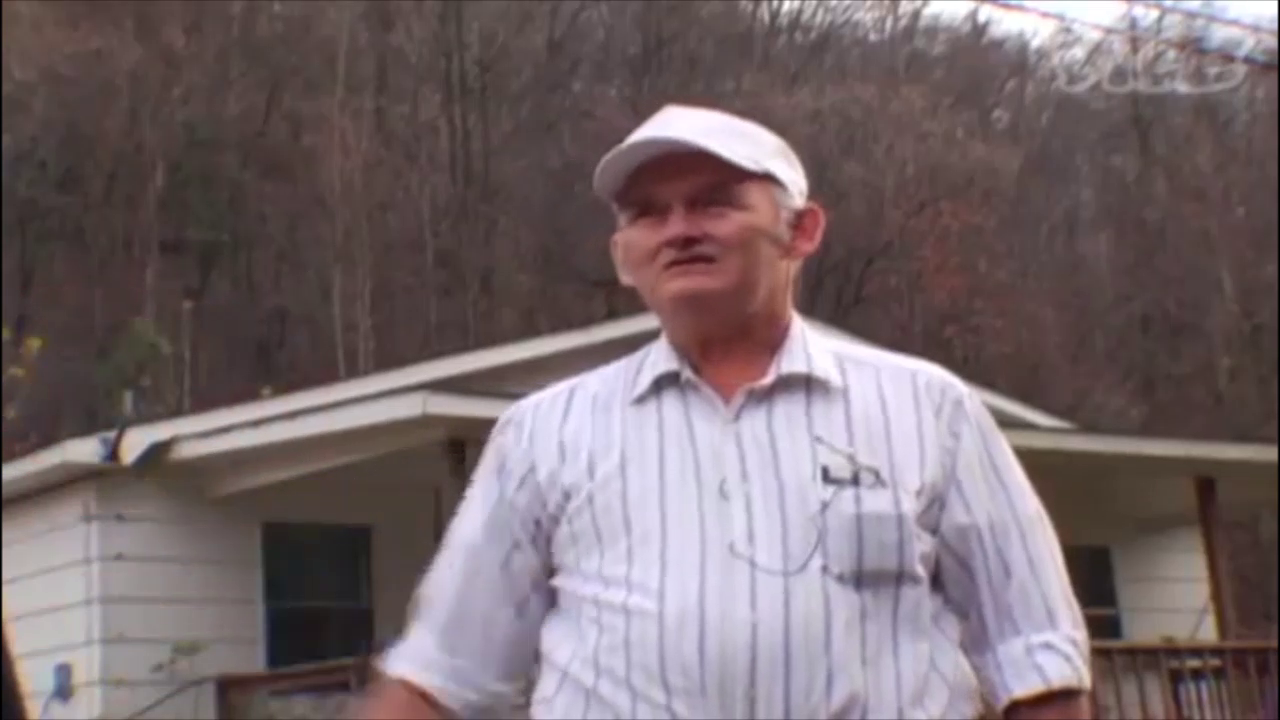
\includegraphics[width=4.2cm]{Figures/mmCult4/frame437.png}  

\end{tabular}
\caption{Cultural level - Example 4}
\begin{footnotesize}
Source: \url{https://www.youtube.com/embed/UvKe2LYy5pk?start=1198&end=1220}
\end{footnotesize}
\label{fig:figure1}
\end{figure}

Early in the segment, we see an open hand palm up gesture similar to that in previous segments. This is followed by a palm up with hands curled inward and index finger and thumb touching. This quickly transitions into a final wave of the hand and gaze upwards with the words ``God can handle this.'' This sequence of movements is a nonverbal juxtaposition between man and God. The finer detailed, downward hand movements (when talking about man) give way to a more spontaneous, upward motion when evoking the spiritual realm. The gaze also shifts upward when referencing God. The words ``he [God] will do what has to be done...'' are accompanied by affirmative nodding. 

The fifth and final cultural-level example features a coal mining worker responding negatively to protesters. In the previous examples, cultural identity is expressed along national, ethnic, or religious lines. In Example 5, culture is expressed in terms of locality and regional (sub-national) affiliation. 

\textbf{\underline{Cultural Level - Example 5}}

\begin{footnotesize}
\texttt{If [they're for us]\textsuperscript{1}, that's good. If they're [against us, get out]\textsuperscript{2} of the state.}
\end{footnotesize}

\begin{footnotesize}
\begin{enumerate}
   \item Hand motion down towards ground, index finger extended
   \item Thumb up; hand motion back over left shoulder
\end{enumerate}
\end{footnotesize}

\begin{figure}[H]
\centering
\begin{tabular}{llll}

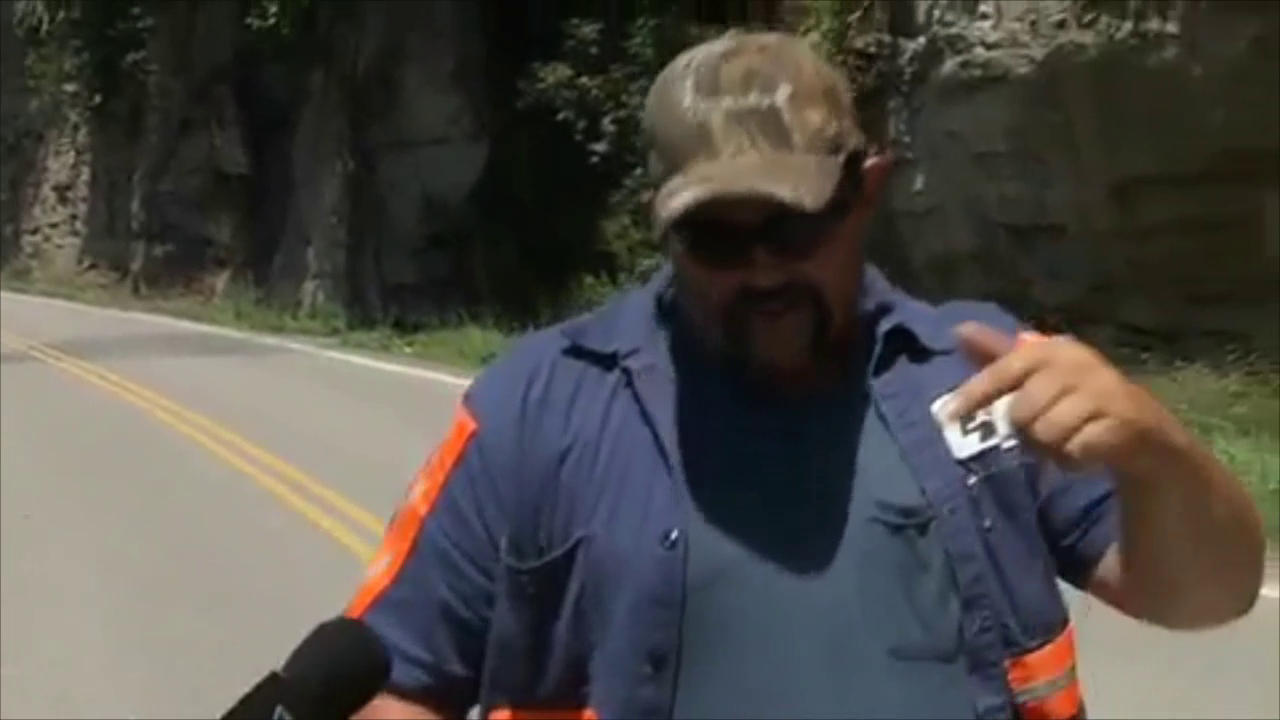
\includegraphics[width=4.2cm]{Figures/mmCult5/frame19.png} & 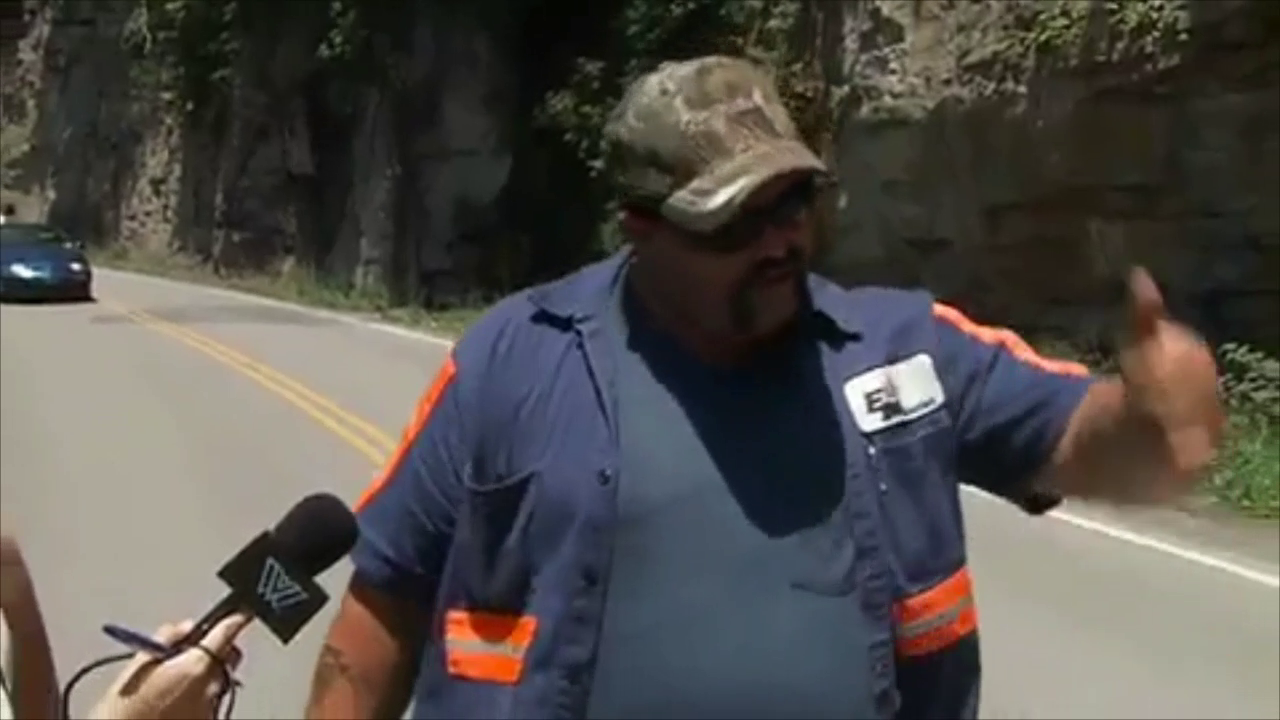
\includegraphics[width=4.2cm]{Figures/mmCult5/frame103.png} & 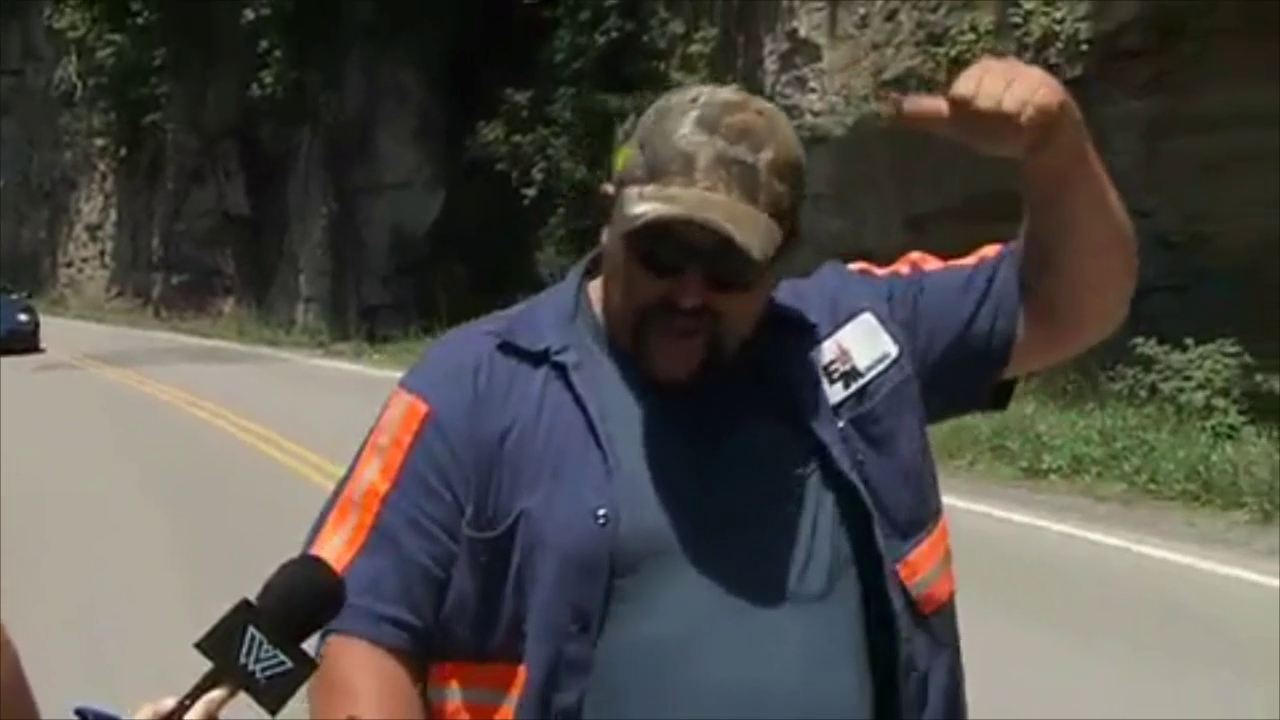
\includegraphics[width=4.2cm]{Figures/mmCult5/frame118.png}  

\end{tabular}
\caption{Cultural Level - Example 5}
\begin{footnotesize}
Source: \url{https://www.youtube.com/embed/vBhvFWRLiOs?start=467&end=476}
\end{footnotesize}
\label{fig:figure1}
\end{figure}

This example shows how in-group/out-group dynamics are embodied in gesture. The words ``if they're for us...'' is accompanied by a pointing downwards in front. When referring to those ``against us,'' the speaker gestures with his thumb over the left shoulder. Using the thumb to point in this way is considered a sign of ridicule and disrespect \citep[140]{Lewis2012}. Thumb displays in general are also associated with expressions of power and authority. Here, the thumb display might be seen as an embodiment of the confidence associated with in-group association.   

\textbf{Summary of Cultural-Level}

What's evident at the cultural-level is an increased animation of nonverbal communication. Hand movements appear more spontaneous and forceful than in the previous, ecological-level examples. Facial expressions and eye movements are also more apparent. The hand movements include markers of emphasis including pointing and on-beat movements. Clenched fist and thumb displays also signal stronger, more emotive communication. Head movements are more pronounced compared to the ecological-level, both through negative shaking and affirmative nodding. Facial expressions include increased blink rates and, in one case, the well known indicator of contempt by raising one side of the lip.   

The cultural-level examples also exhibit a high degree of confidence and affirmation. Pointing, fist clenching, and nodding are signals that speakers believe in their message and affirm it. Similarly, the thumb display in the final example is a high confidence gesture.   

\subsection{Socio-Economic Level}

The socio-economic level features four examples. In these examples, speakers refer to issues of justice, economics, and social institutions. These include a woman speaking about violence surrounding mining projects in Honduras; a woman addressing an audience regarding the need to economic opportunities in their community; a retired miner talking about the lack of institutional regulation towards the coal industry; and a woman stressing the importance of coal mining to her families' livelihood.

Example 1 below is a segment from an interview with a Lenca indigenous woman in Honduras. 

\textbf{\underline{Socio-Economic Level - Example 1}}

\begin{footnotesize}
\texttt{(Translated from Spanish - only gesture annotation)
The worst impacts have been state violence. Why? Because we have comrades who have been killed following military harassment. [We've already lost one person].\textsuperscript{1}}
\end{footnotesize}

\begin{footnotesize}
\begin{enumerate}
   \item Raised eyebrows; wide eyes; extenuated blinks
\end{enumerate}
\end{footnotesize}

\begin{figure}[H]
\centering
\begin{tabular}{llll}
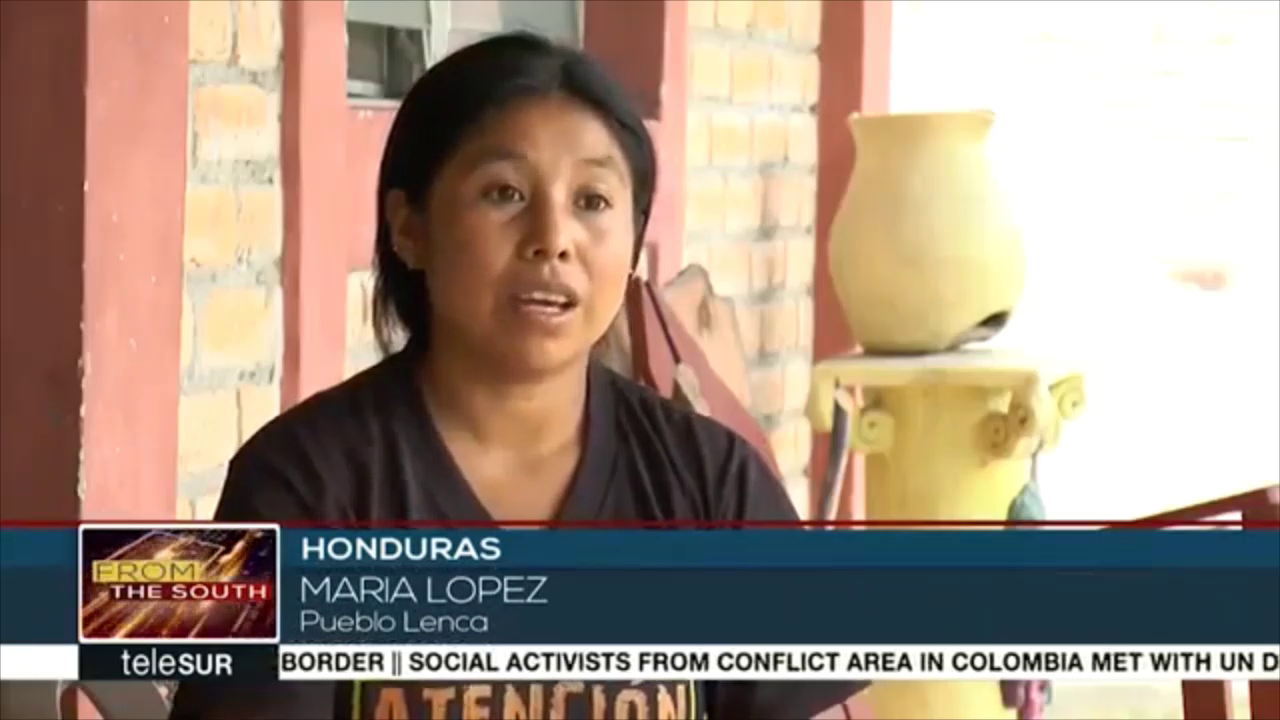
\includegraphics[width=4.2cm]{Figures/mmEcon/frame66.png} & 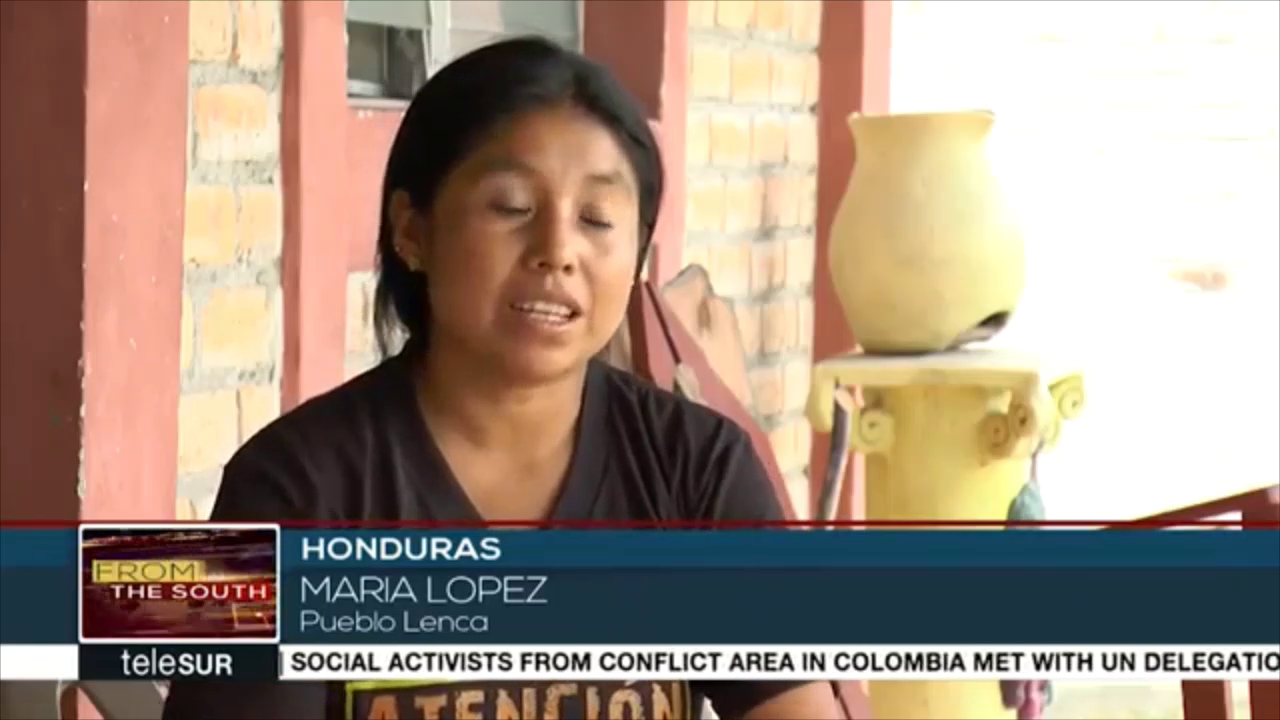
\includegraphics[width=4.2cm]{Figures/mmEcon/frame110.png} & 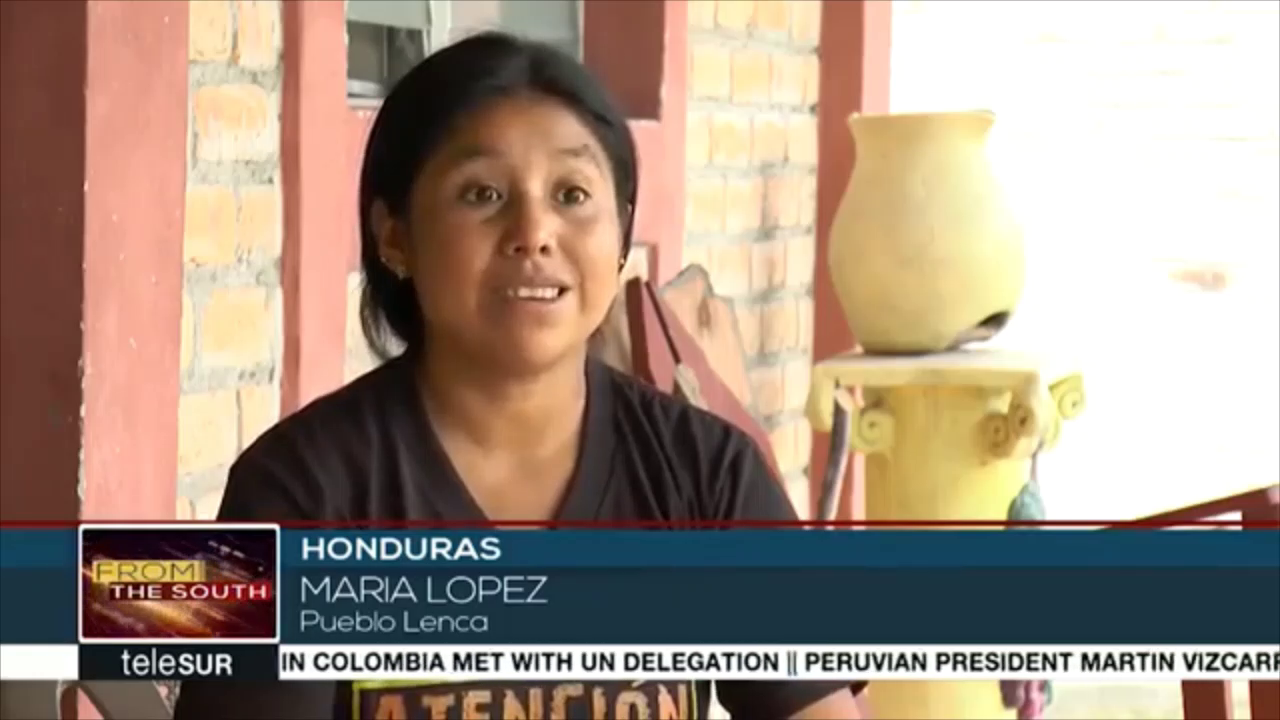
\includegraphics[width=4.2cm]{Figures/mmEcon/frame304.png}  
\end{tabular}
\caption{Socio-Economic level - Example 1}
\begin{footnotesize}
Source: \url{https://www.youtube.com/embed/gU7PBoy-wFE?start=10&end=21}
\end{footnotesize}
\label{fig:figure1}
\end{figure}

In this example, the analysis is largely limited to facial expressions. As she discusses violence and harassment from mining and hydroelectric projects, the eyes and face are strong nonverbal indicators. Particularly in the final frames, the eyebrows are pulled up and together and the eyed widened. The raised eyebrows are characteristic of what's often claimed as a universal facial expression denoting fear \citep[28-30]{Matsumoto2013}. 

Example 2 is unique in that we are able to view body language of listeners as well as the speaker. In this clip a woman is talking about economic hardships in the community in the context of a debate around proposed uranium mining. 

\textbf{\underline{Socio-Economic Level - Example 2}}

\begin{footnotesize}

\texttt{<\annotate{Five years} we'e been trying to keep our doors open, \annotate{thinking} (.) any day now> those jobs were going to be here. >These are the only people that have come in and offered us jobs$\uparrow$< If \annotate{any} of the people here who are against it had come in and [said they had jobs to match it, we'd be behind that too. But right now this is all we've got]\textsuperscript{1}. Everyone one of you who has stood up against this could have brought in jobs [for \annotate{us}.]\textsuperscript{2}}
\end{footnotesize}

\begin{footnotesize}
\begin{enumerate}
   \item Raised and upward slanted eyebrows, stressed blink
   \item Hand points inwards toward chest; index finger extended
\end{enumerate}
\end{footnotesize}

\begin{figure}[H]
\centering
\begin{tabular}{llll}
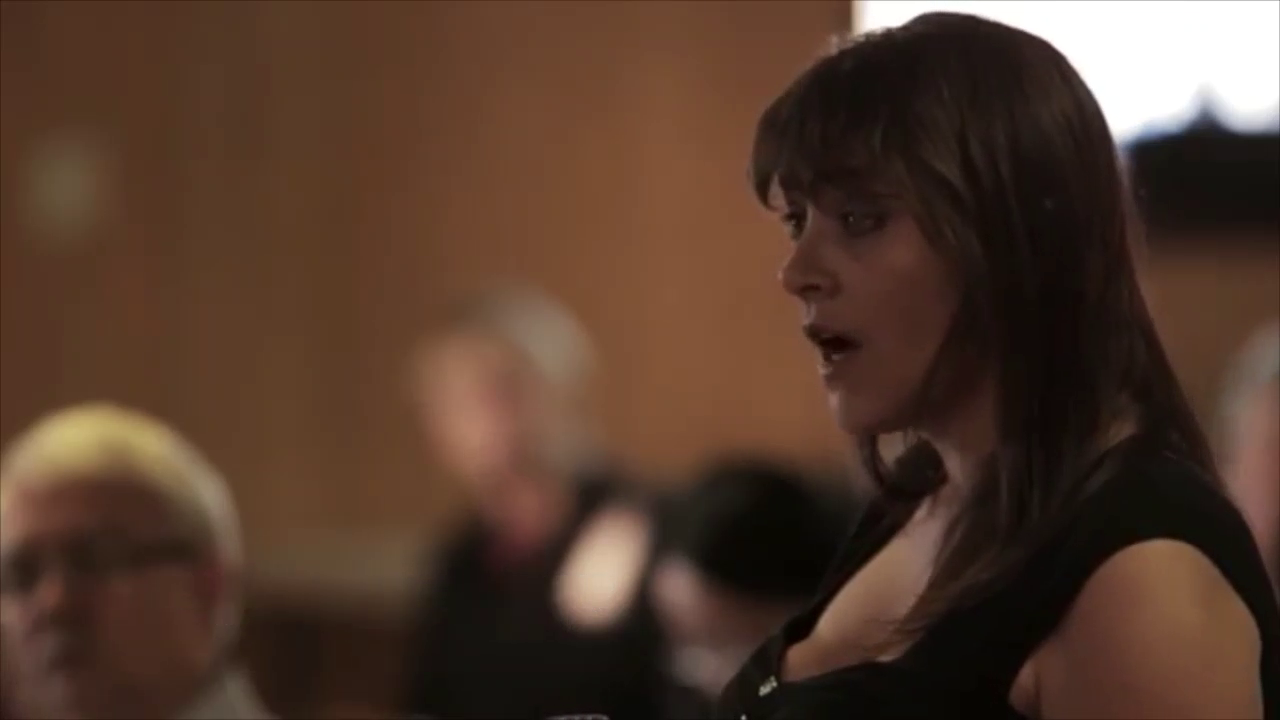
\includegraphics[width=4.2cm]{Figures/mmEcon1/frame413.png} & 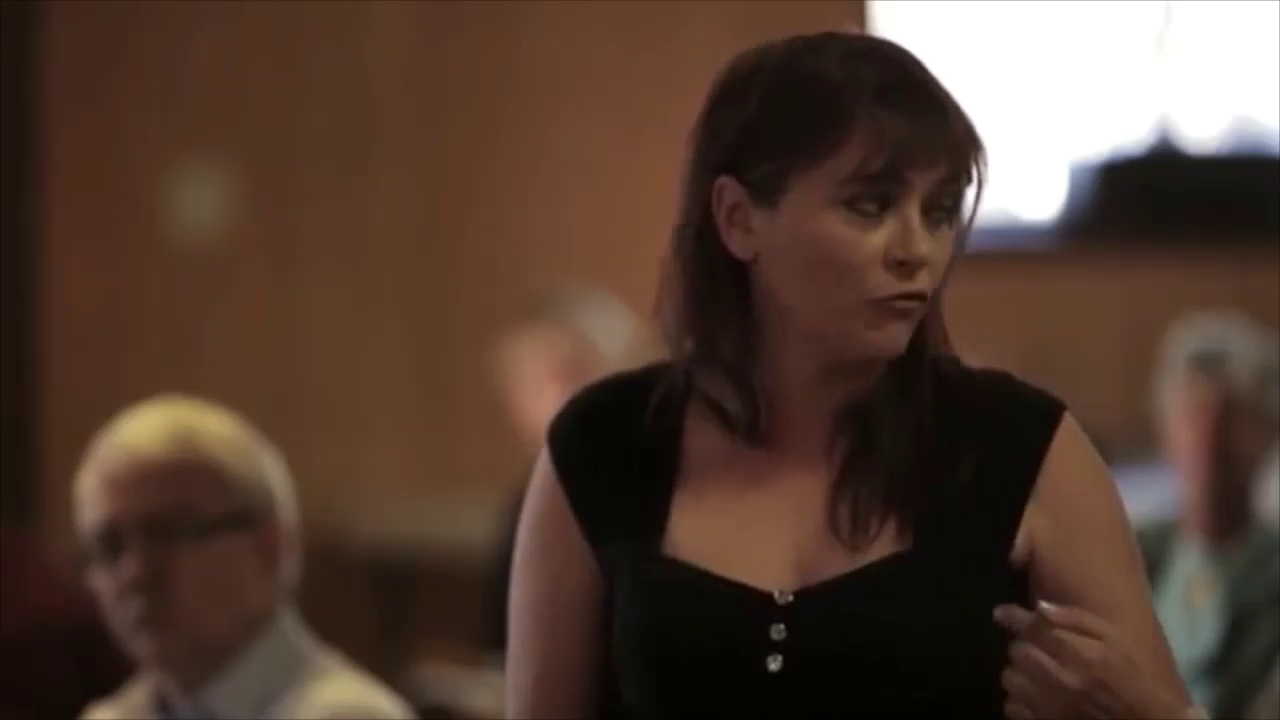
\includegraphics[width=4.2cm]{Figures/mmEcon1/frame725.png} & 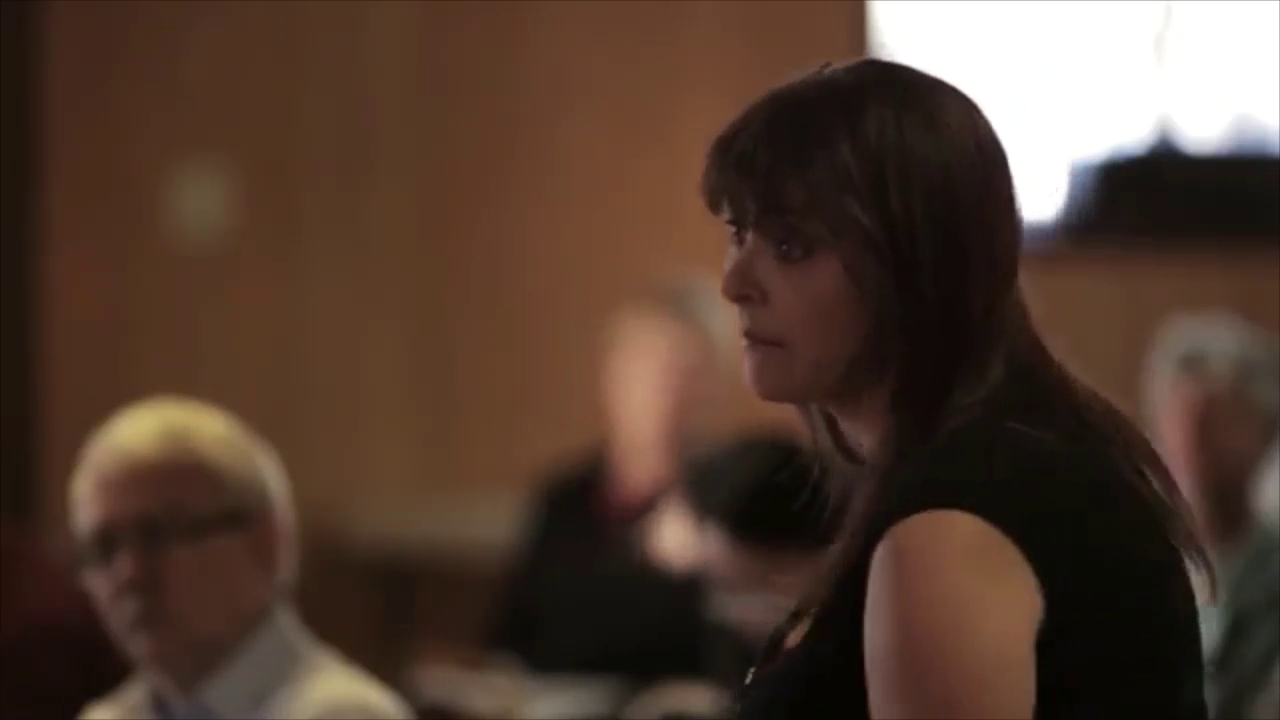
\includegraphics[width=4.2cm]{Figures/mmEcon1/frame988.png}  
\end{tabular}
\caption{Socio-Economic level - Example 2}
\begin{footnotesize}
Source: \url{https://www.youtube.com/embed/Sh0_Wf8F4RM?start=390&end=420}
\end{footnotesize}
\label{fig:figure1}
\end{figure}

\begin{figure}[H]
\centering
\begin{tabular}{llll}
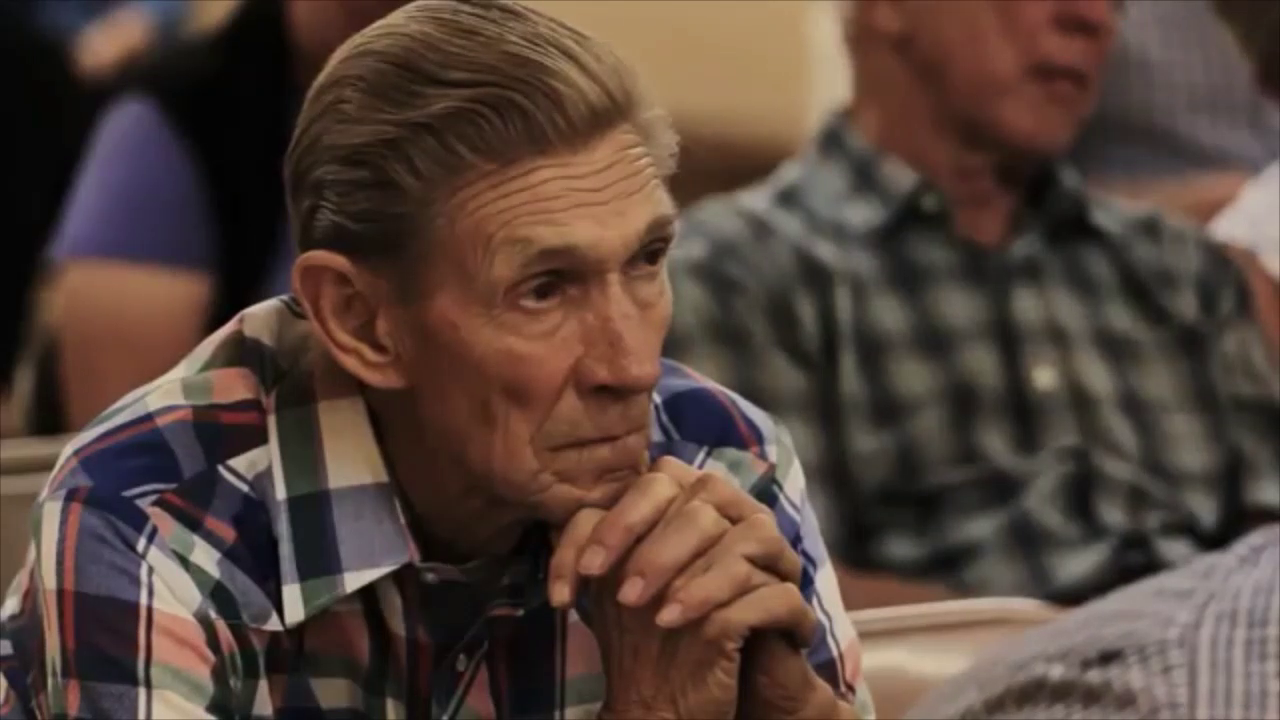
\includegraphics[width=5cm]{Figures/mmEcon2/frame137.png} &  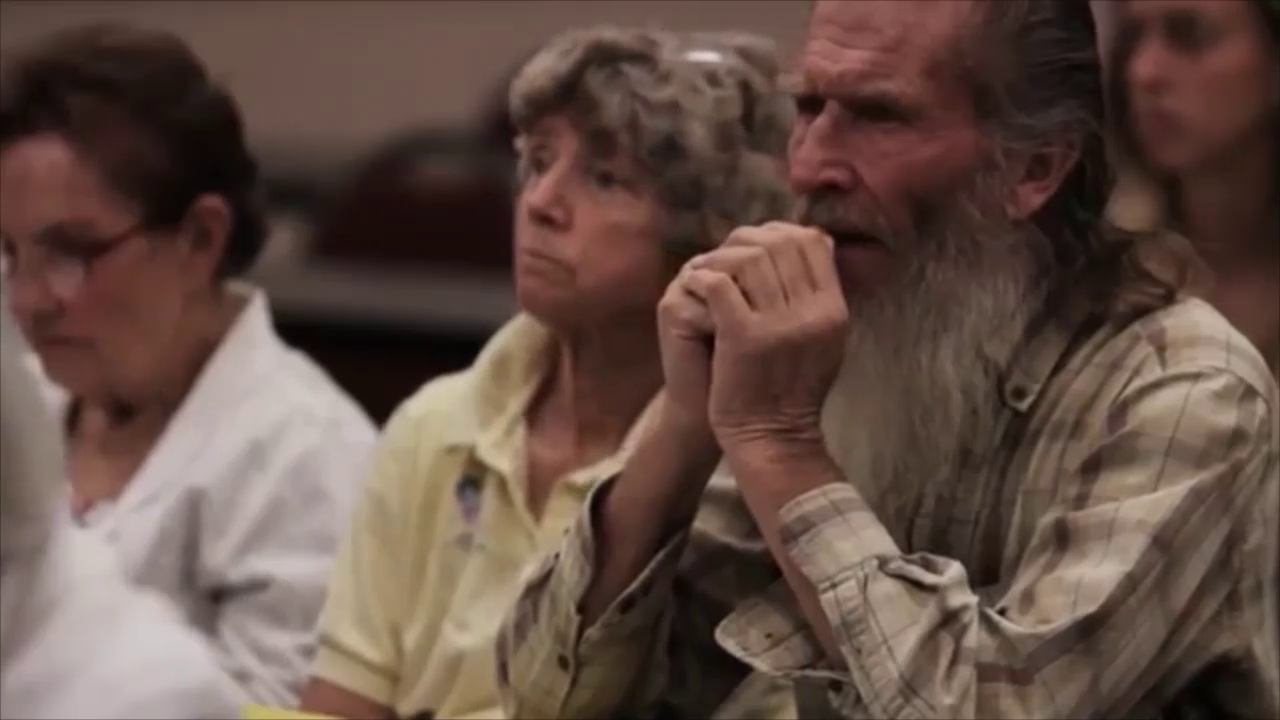
\includegraphics[width=5cm]{Figures/mmEcon2/frame222.png} \\

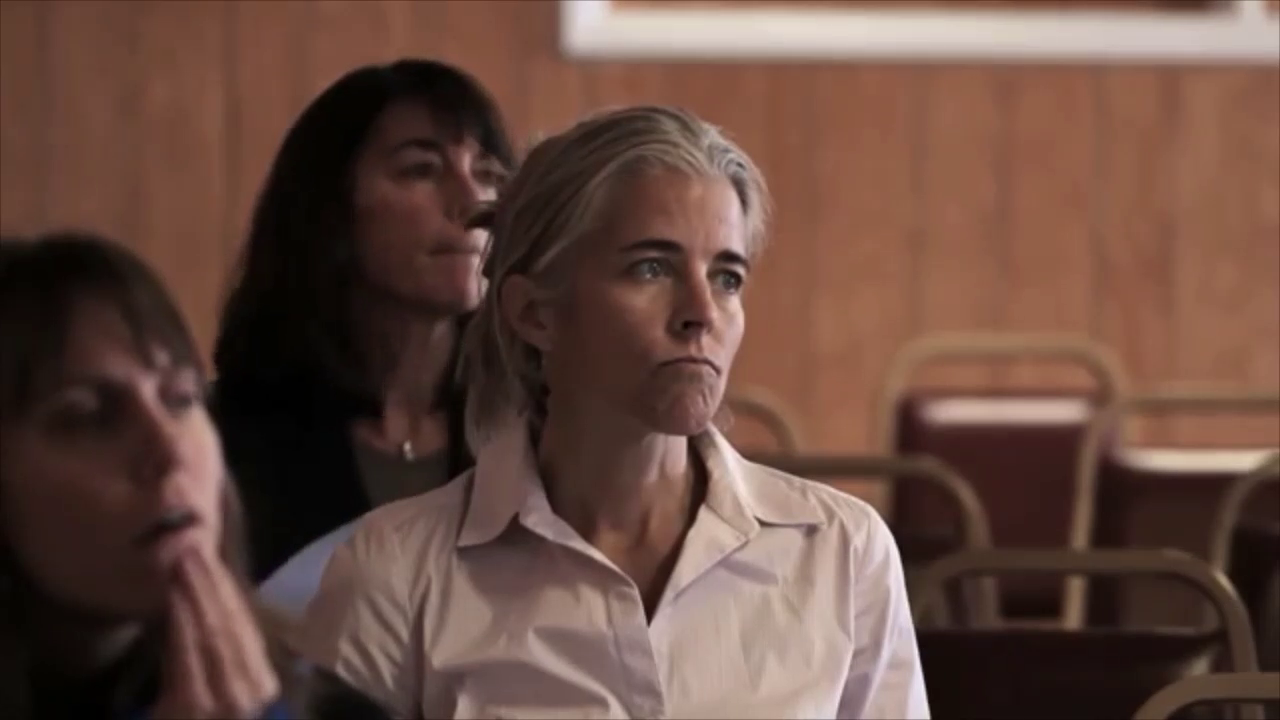
\includegraphics[width=5cm]{Figures/mmEcon2/frame529.png} & 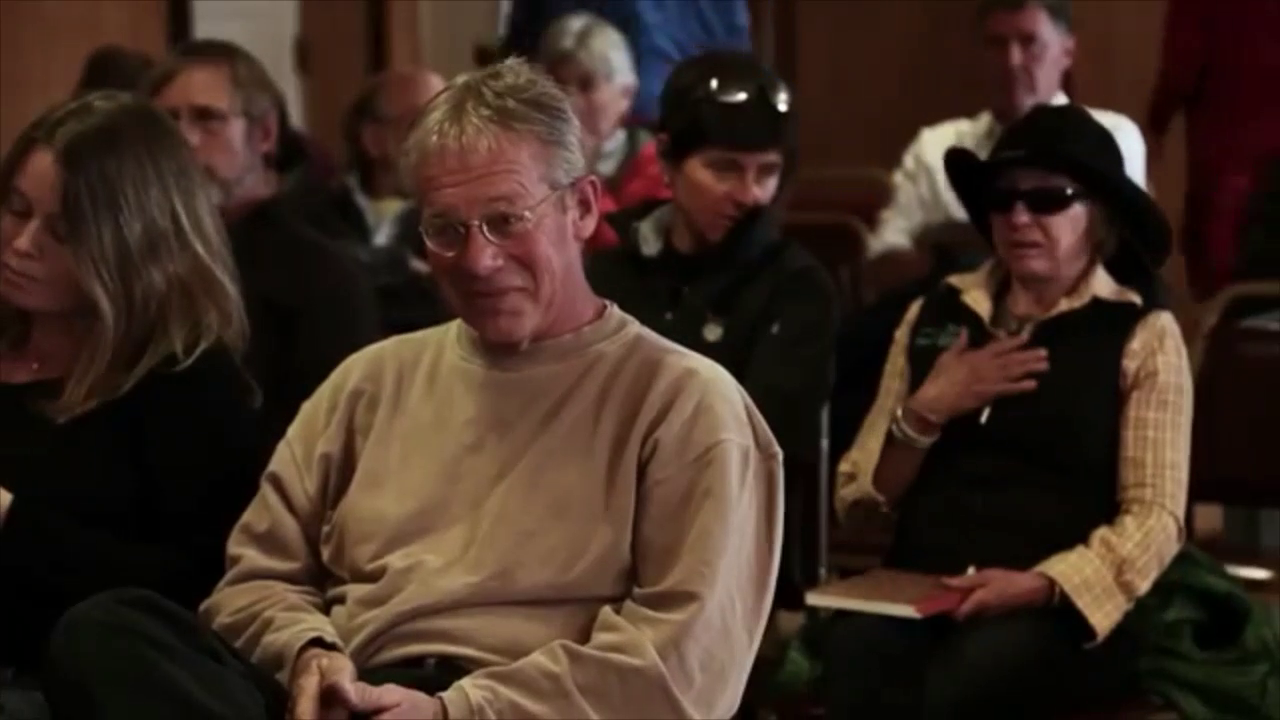
\includegraphics[width=5cm]{Figures/mmEcon2/frame857.png}  

\end{tabular}
\caption{Socio-economic level, listener reactions}
\label{fig:figure1}
\end{figure}

Here we observe an extended blink as well as upward slanted eyebrows. The eyes in particular show concern, worry, and sadness. These expressions are mirrored among listeners. In Figure 5.12 (bottom left) we see a woman with a similar worried and sad expression along with pursed lips. The emotional intensity is apparent given that tearing eyes can be observed, both in the speaker and one of the audience members. Audience members are shown with their hands clenched in front of their faces (Figure 5.12, top left and top right), another indicator of a negative or anxious attitude. On the bottom right of Figure 5.12, we see a man with an obvious expression of sadness as well as a woman behind him with her hand placed on the sternum, a nonverbal expression of empathy.

In this segment, stress and intonation are used more emphatically than in any of the previous segments. For example, in the beginning of the segment, the stress on ``five years'' emphasizes the time duration of hardship. The intonation in the second sentence also conveys a sense of urgency and exasperation. Finally, the stress on the word ``us,'' together with pointing towards the chest, indicates the personal feelings and emotions at play. 

The next example is an interview with a former coal miner on the topic of mountain top removal coal mining.

\textbf{\underline{Socio-Economic Level - Example 3}}

\begin{footnotesize}
\texttt{[They're fighting]\textsuperscript{1} a losing battle I feel (.) myself I feel like they're just fighting a losing battle, because the <[\annotate{politicians}]\textsuperscript{2} and the [\annotate{big} coal companies and things> \annotate{they're} going to win hands down >because the judges and arbitrators are just going to go their way.<]\textsuperscript{3} }
\end{footnotesize}

\begin{footnotesize}
\begin{enumerate}
   \item Both hands extend outward, palms up
   \item Both hands motion forward/downward, palms down
   \item Both hands extend outward, palms up, with emphasis
\end{enumerate}
\end{footnotesize}

\begin{figure}[H]
\centering
\begin{tabular}{llll}
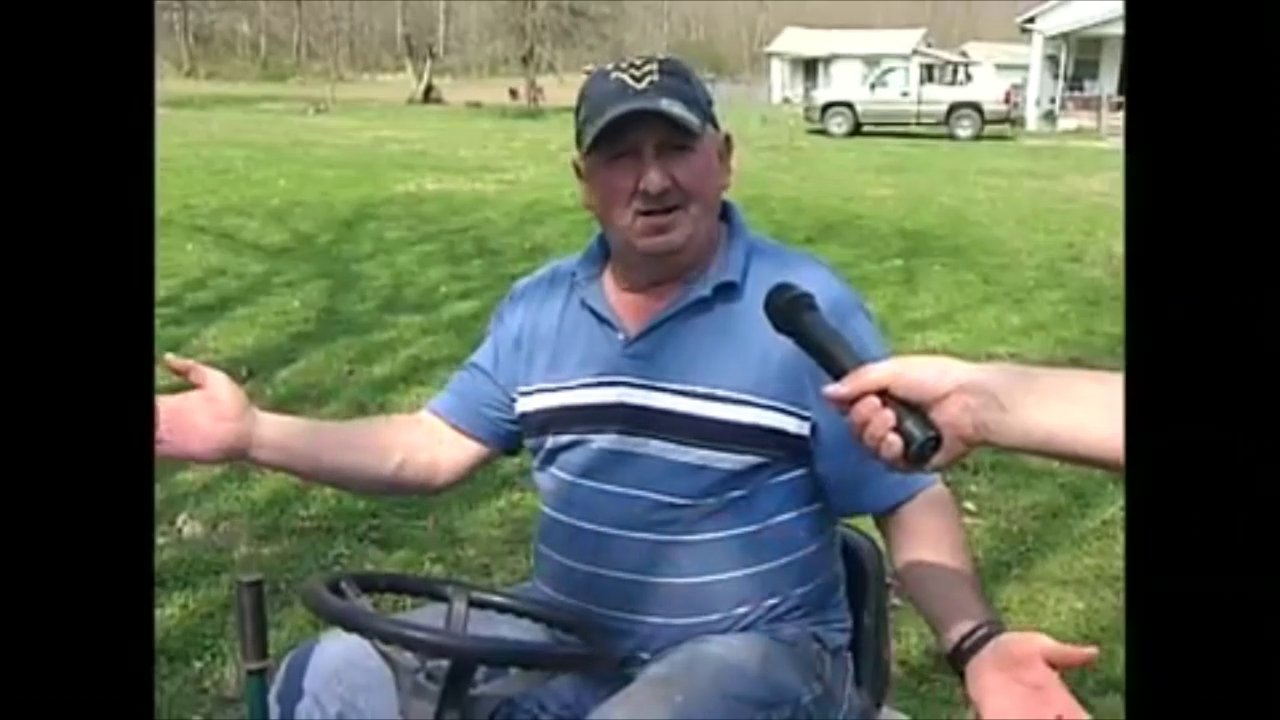
\includegraphics[width=4.2cm]{Figures/mmEcon3/frame189.png} & 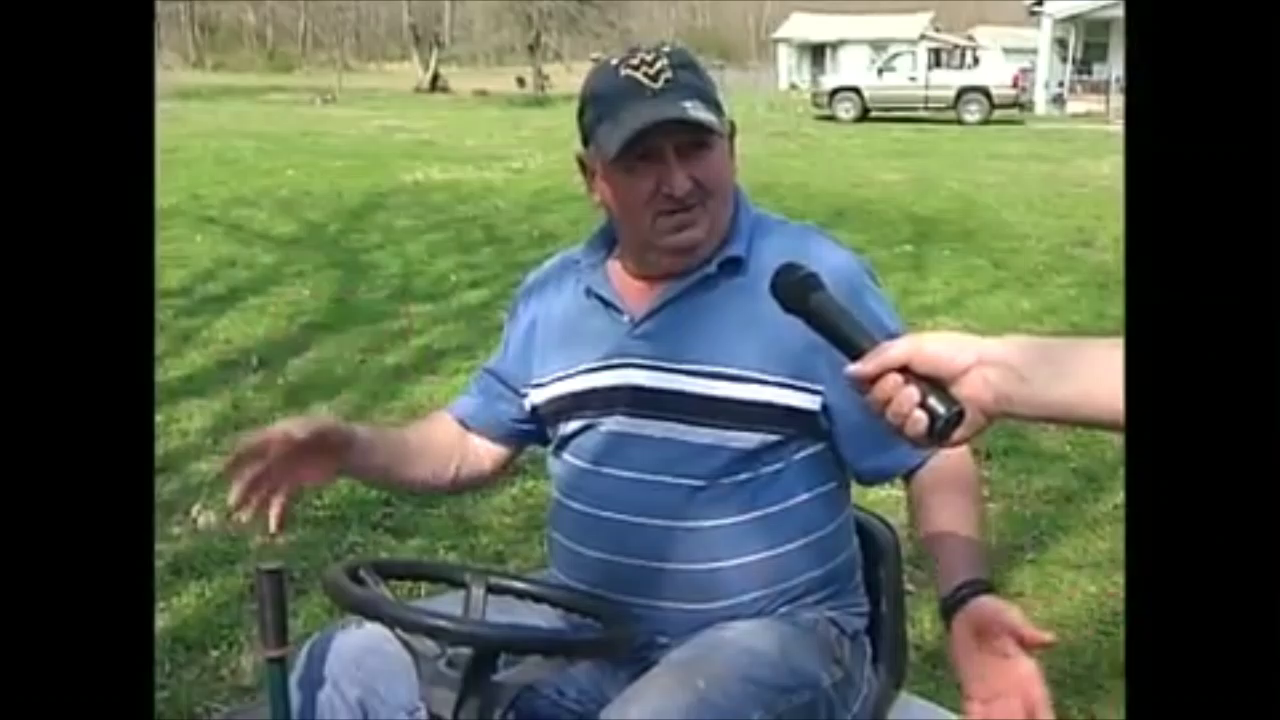
\includegraphics[width=4.2cm]{Figures/mmEcon3/frame450.png} & 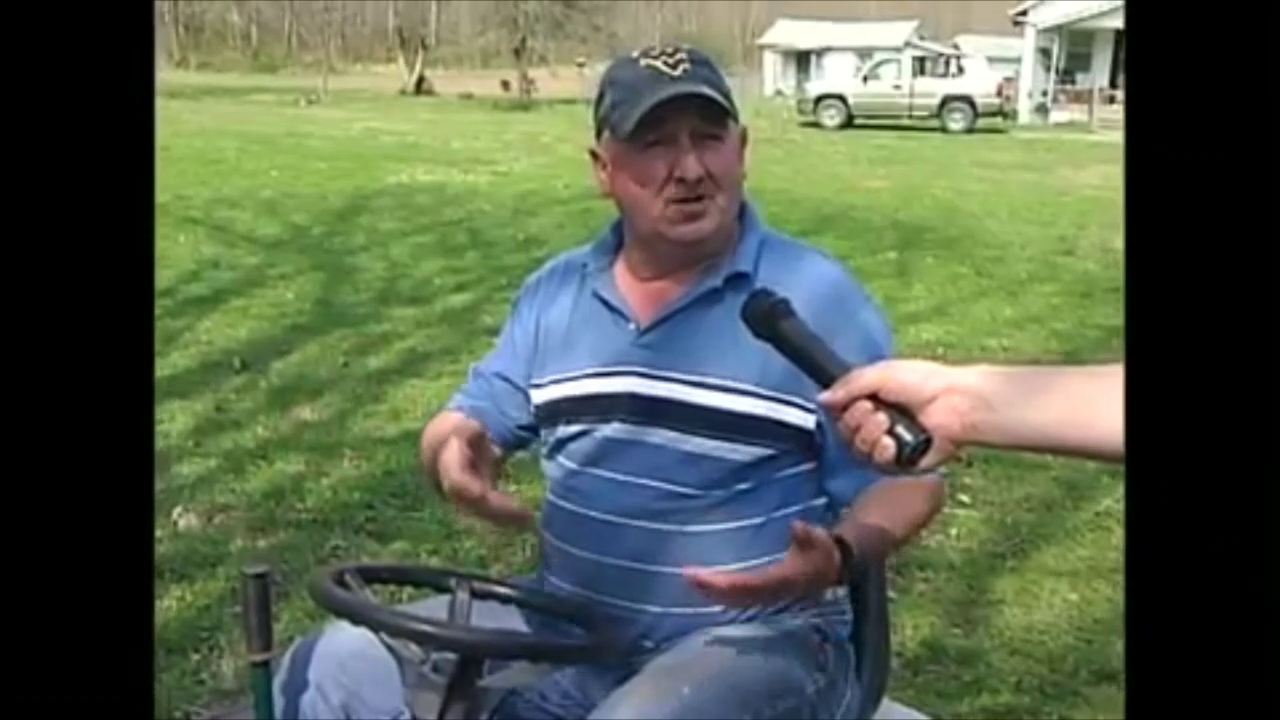
\includegraphics[width=4.2cm]{Figures/mmEcon3/frame610.png}  
\end{tabular}
\caption{Socio-Economic Level - Example 3}
\begin{footnotesize}
Source: \url{https://www.youtube.com/embed/vBhvFWRLiOs?start=1299&end=1316}
\end{footnotesize}
\label{fig:figure1}
\end{figure}

Example 3 exhibits the open hand palm up gesture at various points. At the beginning of the segment the speaker displays an open hands gesture. This open-palm gesture, commonly referred to as a ``pleading'' or ``begging'' gesture \citep[149]{Lewis2012}, depicts a sense of helplessness and resignation. The words ``fighting a losing battle'' complement this sense. The palms-open gesture repeats several times on the stressed words, adding to the sense of futility the speaker is conveying. Briefly, the palm shifts downward to stress the word ``politicians,'' indicating that the speaker is making a strong, assertive point. However, the palms quickly shift upwards for the remainder of the segment. Looking to the facial expressions, we can see eyebrows pinched at the center and sloping downwards. This ``knit brow'' can be interpreted as an expression of worry or concern \citep{Hartley2017}.

The final example is from the same piece on mountain top removal coal mining. The speaker is defending the coal miners and stressing the importance of the industry for her community and family.

\textbf{\underline{Socio-Economic Level - Example 4}}

\begin{footnotesize}
\texttt{If you choose to live in West Virginia, [this is (.) this is the best paying job there is$\uparrow$]\textsuperscript{1}. \textit{Interviewer}: What happens if mountain top removal goes away, what happens to you and your family? \annotate{WE GO HUNGRY!}\textsuperscript{2}}

\end{footnotesize}

\begin{footnotesize}
\begin{enumerate}
   \item Shoulders raise; nodding
   \item Eyebrows raise
\end{enumerate}
\end{footnotesize}

\begin{figure}[H]
\centering
\begin{tabular}{llll}
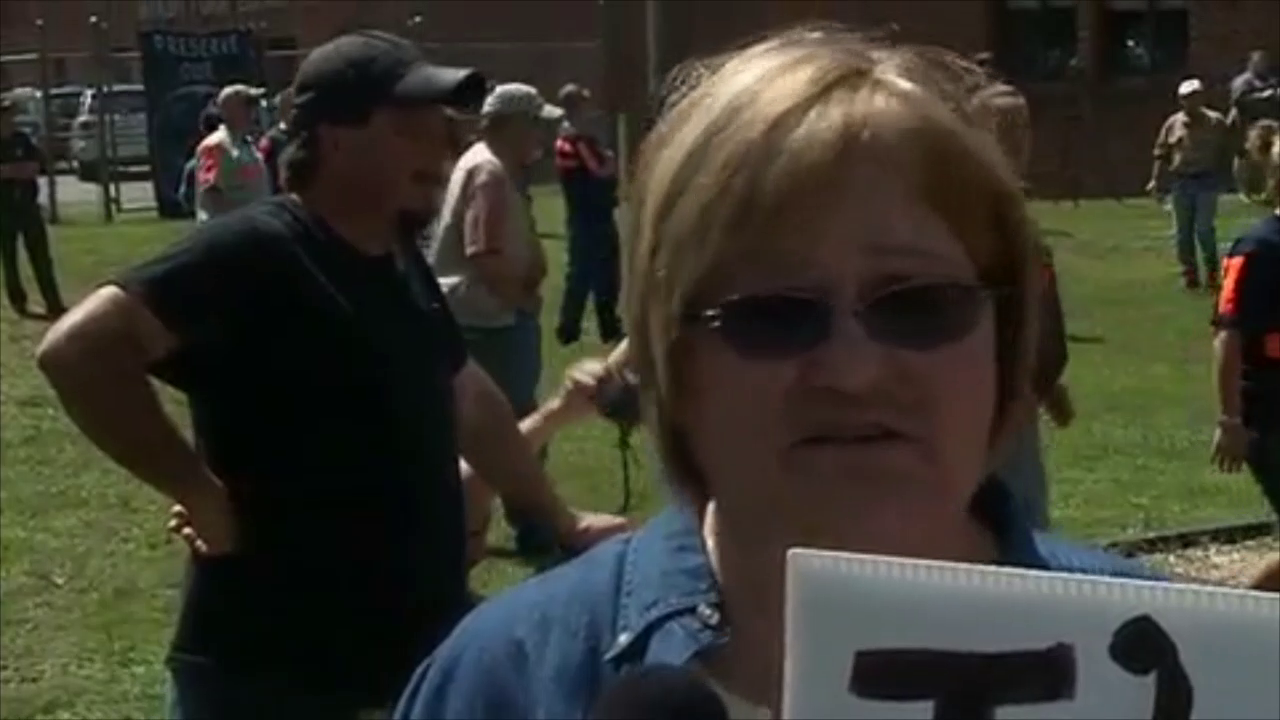
\includegraphics[width=4.2cm]{Figures/mmEcon4/frame3.png} & 
\includegraphics[width=4.2cm]{Figures/mmEcon4/frame551.png} & 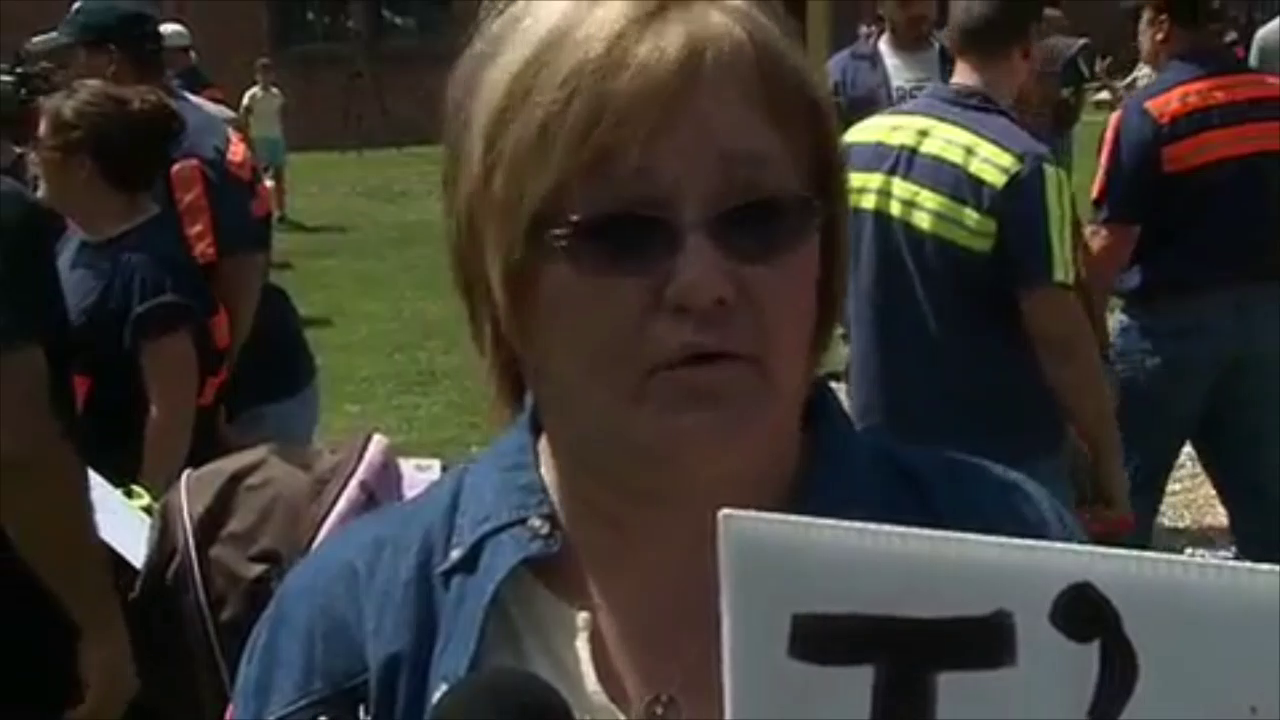
\includegraphics[width=4.2cm]{Figures/mmEcon4/frame901.png}  
\end{tabular}
\caption{Socio-Economic level - Example 4}
\begin{footnotesize}
Source: \url{https://www.youtube.com/embed/vBhvFWRLiOs?start=58&end=75}
\end{footnotesize}
\label{fig:figure1}
\end{figure}

Like in the previous example, the facial expression is one of worry and concern. Coinciding with ``this is the best paying job there is,'' is a shoulder shrug, which can be interpreted as an expression indicating innocence and helplessness, as if to say ``I can't do anything about it'' \citep{Collett2003}. In the final part of the segment, after the question (``what happens if mountaintop removal goes away?''), the facial expression turns to one of surprise with the eyebrows raised, followed by an increased pitch when answering ``we go hungry.'' 

\subsection{Cognitive Level}

The purpose of observing nonverbal communication is to better understand the meaning the speaker is trying to express. Words alone give a partial picture of that meaning, but nonverbals can provide greater insight into thoughts, feelings, and emotions. Whereas, the examples presented are primarily descriptive, this cognitive-level of analysis aims to provide some insights from cognitive science in order to interpret and tie together the various observations.

\textbf{Nonverbal Communication and the Unconscious}

The notion that nonverbals are essential to meaning and communication, is based on premises about the largely unconscious dimension of human cognition. In general terms, these premises are as follows: 

\begin{itemize}
\item Human cognition is mostly (98\%) unconscious, and is inseparable from emotion. Moreover, cognition is embodied, meaning ideas, language, and even thought are mediated by the body \citep{Lakoff2010a}. 
\item Human needs, emotions, and intentions are processed by the limbic brain. Nonverbal communication and, in particular, body language is to a large extent the expression of unconscious limbic processsing \citep{Navarro2008,T.Lamendella1977}. Gestures are expressions of embodied cognition \citep{Kinsbourne2006}.
\item In contrast to nonverbal communication, human (verbal) language abilities are more consciously driven and concentrated in the frontal lobe of the brain, which is responsible for thinking, planning, and judgment.     
\end{itemize}

In essence, cognition is mostly unconscious, it is inseparable from the body, and is expressed through embodied communication. It follows that nonverbals convey thoughts, feelings, and emotions in ways that speech alone does not. Nonverbals are often not inhibited and regulated in the same way as speech is, in the cortical and frontal lobe areas of the brain. Of course, this is a simplification. A more comprehensive review of the cognitive neuroscience of human communication is beyond the current scope. In reality, complex interactions occur between areas of the brain \citep[32]{Wood2005}. Nonetheless, the basic point is that the importance of nonverbals to discerning overall meaning is rooted in human cognition itself. Nonverbal communication is required to understand the full communicative intent, which encompasses emotions and reactions as well as thinking and judgment. 
 
While nonverbals can be deliberate and intentional, they often occur without our conscious awareness and, thus, are explicable in terms of the limbic system. Involuntary facial expressions, for instance, originate in the subcortical areas of the brain \citep[36]{Matsumoto2013}. There is also evidence to suggest that head movements encode emotional intent \citep{Livingstone2016a}. In fact, the very definition of gestures (as opposed to sign language or emblems) is that they are generated without conscious awareness \citep[9]{Beattie2016}.

\textbf{Emotional Expression}

Another key point is that nonverbal communication is closely associated with the site of emotional processing, the limbic system. As discussed in Chapter 4, sensory information is first processed by the amygdala (part of the limbic system) before further processing by the cortex. As \cite{LeDoux1994} explains:

\begin{quote}
Visual information is first processed by the thalamus, which passes rough, almost archetypal, information directly to the amygdala. This quick transmission allows the brain to start to respond to possible danger. (56)
\end{quote}

In this way, emotions serve an important cognitive evolutionary function by allowing for rapid information processing with minimal deliberation \citep{Tooby2008}. In contrast to the classical Enlightenment ideal of rational human thinking, emotions are inseparable from cognition \citep{Lakoff2010a}.

It should be noted that there is not universal agreement that nonverbal communication is a reflection of internal emotions. With respect to facial expressions, \cite{Crivelli2018} explain that, according to the behavioral ecology view of facial displays (BECV), facial displays are tools for social influence. The BECV contrasts with the basic emotions theory (BET), which holds that facial expressions reflect internal emotions. However, as \cite{Lakin2006} points out, the behavioural ecology view offers a different explanation for what we call emotions, but is still compatible with the view that facial expressions often occur without conscious awareness (65). 

One general conclusion from the examples presented in the previous section is that, in comparison with the ecological level, emotional expression seems to be more pronounced in the cultural and socio-economic levels. This conclusion is based on qualitative interpretations of clusters of nonverbals. However, to break down how one could arrive at this conclusion, we can consider facial displays in more detail.  

\textbf{Cognitive-Level Interpretation of Facial Expressions}

Psychological research has suggested there are universal facial expressions (UEs), which correspond to the ``six basic emotions'' proposed by \cite{Ekman1971} and \cite{Ekman1972}: happiness, surprise, disgust, sadness, anger, and fear. This early research also notices cross-cultural variability in facial expressions, attributed to ``display rules'' regarding emotional expression which are learned in the context of one's culture. Recent research has challenged the universality hypothesis by finding there are distinct differences in the way people from Western and Eastern cultures display and recognize the six basic emotions. There is also evidence of cultural variability in parts of the face used to express emotion. For instance, \cite{Jack2012} find that East Asian models of emotions find more intensity in the eyes. This conclusion makes sense in terms of a hypothesis that East Asian cultures learn to be more inhibited in the expression of emotion and the eyes, which are generally subject to less voluntary control than the mouth \citep{Mai2011}, are better indicators of emotional expression.

In the context of the examples presented, the primary implication is that interpretation of facial expressions is just that: an interpretation. There are some general, perhaps universal characteristics, but the expression and interpretation of emotion also varies with the culture of speakers/observers. One way to account for cultural variability, however, is to pay particular attention to the eyes.

In the ecological-level examples some facial expressions were noted. However, these can generally be interpreted as expressing lower degrees of emotion than those seen at the other levels. In the first example, for instance, the speaker has what might be described as a ``neutral face,'' characterized by either a low degree of emotion or an expression in its own right whose emotional meaning is contextual \citep{Carrera-Levillain1994}. Given the context of the first example (scientist discussing research), the neutral expression fits with the social and professional expectations of the communicative context. Accordingly, we might conclude that there is relatively low emotional reaction in this segment. This conclusion is supported by the content of the speech, which indicates the speaker is also engaged in non-binary thinking by outlining that there are grey areas about the ecological impacts of deep sea mining. Non-binary thinking is an indication that, rather than an automatic response from the amygdala, there is emotional modulation via the cortex, which manifests as exploring and considering different options or reactions \citep{Wood2005}.    

Another indication of emotional modulation is the upward motion of the eyes, which can be seen in the ecological as well as the cultural examples. This, again, is a possible indication of engagement with rational thinking and the cortex (as opposed to the automatic response of the amygdala). Research suggests looking upward is associated with spatial and verbal memory recall \citep{Nespoulous2014}. Whereas emotional ``fight or flight'' responses dilate the pupils to increase visual information, the opposite might also be the case when engaging in abstract thinking with the prefrontal cortex; that is, a relaxing of the gaze and limiting the visual information in order to free up cognitive processing for information retrieval.

In the cultural-level examples, we also see evidence of more emotional responses. The higher degree of emotion is not surprising given that these speakers are addressing identity and intergroup relations amid sensitive topics. As mentioned, cultural Example 2 contains a ``sneer,'' which is often said to be an expression of contempt \citep{Izard1988}. In cultural Example 3, the speaker displays a high blink frequency and blink duration, which is a possible sign of negative emotional states including stress \citep{Haak2019} and fear \citep{Maffei2019}. Thus, at the cultural level we see a mix of emotions by way of facial expressions.

Emotional facial expressions are perhaps most pronounced at the socio-economic level. Unique to this level are the expressions of sadness, worry, and concern. Sadness is generally associated with oblique eyebrows and pulling down of the lip corners \citep{Duran2017}. This expression is apparent in socio-economic Example 2, which is unsurprising given that the topic in this segment is unemployment and economic hardship. Also, in the same segment we see watery eyes and possible tearing. In adults who generally have developed empathy, tearing is often triggered by the suffering of others \citep{Murube1999}. In the same example, we see listeners exhibiting similar emotional responses. At the cognitive-level, the listener responses can be seen as an example of how emotions elicit a ``mosaic'' of mirror neurons causing the observer to experience similar feelings as the person who expressed the emotion \citep{Bastiaansen2009}. 

\textbf{Cognitive-Level Interpretation of Gestures}

In addition to different facial expressions, the three levels of analysis (ecological, cultural, and socio-economic) also exhibit differences in the gestures displayed. As mentioned, in the ecological-level there is a notable use of iconic gestures, which closely reflect literal spoken words, at the interface of imagistic and linguistic representation \citep{Ozyurek2010}. As speakers begin to address cultural and socio-economic topic, the gestures become less iconic and more metaphorical. At these levels, the emotional intensity increases. How we can interpret something that is seemingly subjective (i.e. the emotional intensity of gestures) is outlined by \citeauthor{Kinsbourne2006} (\citeyear{Kinsbourne2006}) as follows: 

\begin{quote}
When gestures are driven by emotion they become less discrete, and may
occur in concert with postural shifts and facial expressions that incidentally emphasize and clarify the meaning that is being communicated. (208)
\end{quote}

In other words, when a speaker is more emotional, their gestures often increase in amplitude, pace, or frequency. That said, it is not gestures alone that convey the emotion, but gestures in conjunction with other nonverbal signals. 

The ``discrete'' gestures we see in the ecological examples communicate spatial relationships in close relation to semantic information. The speakers are often describing physical processes, such as the directional pointing in Example 2 or water well spigot inspection (Example 3). These gestures are controlled, deliberate, and match the literal semantic information. 

By contrast, in the cultural examples gestures become more metaphoric. They emerge in conjunction with more abstract topics including culture, fighting back, or in-group/out-group identities. The same can be said with respect to the socio-economic examples, but with an important distinction: the cultural examples are often expressions of power, confidence, and assertion. For instance, we see palm down motions, pointing, a fist pump, and thumb displays. However, in the socio-economic examples we are more likely to see expressions of hopelessness and innocence. These include several instances of the palm open ``pleading'' gesture, as well as the shoulder shrug, and the hand covering the chest.      

\textbf{Summary of the Cognitive Level}

The observed trends in facial expressions and gestures suggest that different cognitive responses are exhibited at different levels of discourse. The ecological level exhibits more verbal and spatial reasoning and does not appear to trigger emotional responses. In other words, the ``fight or flight'' emotional responses of limbic system and subcortical areas of the brain are being mediated. The cultural level seems to trigger emotions, but these are generally high confidence, one could even argue dominant, nonverbal signs. This might be attributed to in-group identities that are being asserted. Finally, the socio-economic level is more likely to display low confidence gestures. The sense of exclusion and vulnerability in the face of threatened livelihoods is one possible explanation for these responses.

\section{Summary \& Conclusions}

Nonverbals are not merely an important part of communication to consider alongside speech; they are inseparable from the message itself. This chapter aimed to look at communication in a holistic sense, with verbal and nonverbal communication as part of an integrated flow. However, if there is a point at which we can distinguish nonverbals from verbal communication, it is with respect to their relation to cognition and emotions. As \citeauthor{Beattie2016} (\citeyear{Beattie2016}) points out, with nonverbal communication ``meaning has not been controlled and self edited by the speaker'' (16). In other words, the nonverbal messages are reflective of mental processes and emotions, in ways that words alone are not.

The most notable conclusion from this chapter is that different discursive levels corresponded to different types of nonverbal displays, as outlined in Table 5.2 below. These differences can be summarized as follows:

\begin{itemize}
\item Speakers at the ecological level generally show less facial expression. Gestures are predominantly iconic and depicted physical/spatial processes. Compared to the other levels of analysis, intonation and stress are less pronounced.  

\item Speakers at the cultural level display more power and confidence gestures, including pointing (to add emphasis), thumb displays, and fist pumping. Gestures are more metaphoric than in the ecological level, depicting abstract concepts such as God, culture, identity, and fighting back. Contempt and agitation are displayed, at one point by the contempt expression (raised side of mouth) as well as the backwards thumb gesture on another occasion.

\item The socio-economic level displays a high degree of emotion, often expressed in the eyes. Universal facial expressions of fear and sadness can be seen in the speakers and, in one case, among listeners. Gestures also indicate hopelessness and innocence, such as the palm open ``pleading'' gesture as well as the shoulder shrug.  \end{itemize}

\begin{table}[H]
\centering
\begin{footnotesize}

\begin{tabular}{ | P{3cm} | P{3cm}| P{3cm} | P{3cm}| }  
\hline
\textbf{Level}          & \textbf{Gestures} & \textbf{Facial Expression} & \textbf{Paralanguage} \\ \hline
\textbf{Ecological}     &  Iconic; depicting physical processes (directional pointing, hand motions)                & Minimal emotional expression; some eyes looking upwards (thinking expression)                           & Minimal stress and intonation                      \\ \hline
\textbf{Cultural}       & Metaphoric; depicting power, confidence, and assertion (palm down, pointing, fist pump, thumb displays)                 &    Contempt displays; anger; agitation (sneer, higher blink rate, audible inhalation/exhalation)                         &  Stress on key points; more variation in speed of speech                     \\ \hline
\textbf{Socio-Economic} &  Hopelessness and innocence (palm open, shoulder shrug; hand on chest)                &     Sadness, concern, worry, fear (raised eyebrows, teary eyes, eyebrows pulled together)                        & Stress; intonation; more changes in pitch                       \\ \hline
\end{tabular}
\caption{Summary of nonverbal communication observations}
\label{tab:my-table}
\end{footnotesize}
\end{table}

It appears that emotions and unconscious attitudes vary when it comes to environmental issues. Specifically, when one's cultural identity or socio-economic status are at stake, these attitudes intensify. When ecological issues are decontextualized from identities or livelihoods, the opposite seems to occur. \citeauthor{Beattie2016} (\citeyear{Beattie2016}) discusses similar observations in terms of implicit and explicit attitudes towards environmental issues:  

\begin{quote}
    The vast majority of people say that they really do care about environmental issues...yet... \textit{sometimes} there is something about the form and nature of their hand movements...which might suggest otherwise. (19, original emphasis)
\end{quote}

In other words, there is a discrepancy between what people consciously know they \textit{should} care about, and how they unconsciously feel. 

This discrepancy has great relevance when it comes to raising awareness about, and addressing, ecological issues. The implication is that communication matters a great deal when it comes to the environment. Specifically, mobilizing people to address ecological issues will depend on framing these issues in a way that speaks to their implicit, unconscious attitudes. From a cognitive science perspective, \citeauthor{Lakoff2010a} (\citeyear{Lakoff2010a}) makes this point and advances some implications for environmental communication, namely

\begin{itemize}
\item The importance of discussing environmental issues in terms of moral values.
\item The efficacy of stories and narratives as opposed to statistics and bland facts.
\item The necessity to address everyday concerns and avoid technical jargon. (79-80) 
\end{itemize}

The observations in this chapter support these points. However, the point about ``moral values'' might be expanded to encompass cultural identity and worldviews. The examples in this chapter show multiple ways in which culture emerges in environmental debates, and how issues becomes impassioned when this occurs. Also, the necessity to address ``everyday issues'' is underscored by the importance of framing issues in terms of economic livelihoods.     
 % Analysis 3

\chapter{Conceptual Framing and the Ecological Turn}
\lhead{\textit{Conceptual Framing and the Ecological Turn}}

\textit{\textbf{Chapter Summary:} This chapter turns back to the research problem stated in Chapter 1, namely, to identify conceptual principles to integrate intercultural communication and ecology. It is argued that the thought of two twentieth century philosophers, Ludwig Wittgenstein and Hannah Arendt, provide rich concepts and vocabulary to this end. To help operationalize these concepts, the four levels of discourse are revisited by outlining \textit{concepts of discourse} and \textit{aims of analysis}.}
\newline

The three analyses in the preceding chapters differ vastly in terms of types of linguistic data as well as topics discussed. Analysis 1, which covers GM seed, spans different geographic locations and is concerned with nature at the molecular scale. Analyses 2 and 3, by contrast, focus more on specific times and geographic locations, at the scale of the built environment of raw materials and infrastructure. The communication data also vary widely between the analyses, from the level of whole texts (Corpus 1), to verbal utterances (Corpus 2) and, finally, nonverbal microexpressions (Corpus 3). Following these three analyses, we return to the question of what conceptual principles can guide our understanding of human communication in relation to the natural world. This present chapter integrates the analyses and begins to sketch out conceptual aspects of the topic. 

In each of the analyses, there are a complex array of issues and factors to consider. The multilevel method sheds light on the sheer breadth of these issues. If nothing else, a takeaway from the analyses is that issues at the interface of the natural environment and human cultures are complex and multifaceted. On the one hand, understanding the interface between humans and the environment requires interpretive approaches based on humanistic inquiry to grasp the experience [\textit{Erlebnis}] of what a given environmental issue means for different groups and communities. On the other, viewing issues through the lens of humanistic inquiry alone is not sufficient. Often the issues concern economics, power, and resource distribution, in which case more social scientific inquiry is called for. Beyond both humanistic and social scientific inquiry there is a crucial role for empirical science as the bedrock for understanding ecological issues. 

Thus, at the outset, we are confronted with the basic question of how to combine modes of inquiry in a way that allows for the study of the natural world alongside human cultures and communication. ICC research generally draws from social scientific or humanistic modes of inquiry \citep[see][]{Littlejohn2011a}. By contrast, any theoretical approach to the natural environment would almost certainly refer to the natural sciences. Cultural and communication studies are often based on constructionist, postmodern premises which often clash with the objective and empirical aims of the natural sciences. Without compromising the role of the scientific argumentation and empirical evidence in both understanding and addressing ecological issues, there is also a need for meaning-centred approaches to the natural world. In other words, environmental issues are not only questions about scientific evidence and theories about nature; they also concern how nature is experienced, interpreted, and is a source for meaning.

One can begin to see the need for interdisciplinary approaches. However, without shared principles and concepts, such approaches are unlikely to succeed. The question then becomes, what are unifying concepts that can serve as a departure point for understanding the interface between intercultural communication and environmental issues?

In seeking this conceptual orientation there are certain criteria that can serve as a starting point. First, it is advantageous if the approach is anti-essentialist and capable of dealing with fuzzy categories, but not at the cost of a consistent and realistic critical stance. Second, the orientation should be reflexive and modest with respect to our own epistemological position. Finally, given calls to de-westernize communication theory and discourse studies \citep[e.g.][]{Shi-xu2005a, Tapas2012a, Waisbord2014a}, a range of intellectual traditions should be considered. In short, the researcher is engaged in an open, non-reductive intercultural philosophy \citep[see][]{Mall2000a}.

By combining intercultural and ecological themes, we are grappling with two broad features of both human societies and natural systems: plurality and complexity. Plurality refers to the uniqueness and variety of cultures, languages, and lifeforms. Complexity refers to the manifold ways in which these phenomena combine, evolve, and interact. We are especially interested in how plurality and complexity are reflected and embodied in human communication. To begin to outline conceptual principles, we turn to two thinkers. The first is Ludwig Wittgenstein; notably, concepts from his later philosophy such as language games and unsurveyability. The second is Hannah Arendt, more specifically her notions of the plurality and the public sphere.

\section{Language Games}

A key question that emerges from the analyses is how to understand the varied complexities of human languages, cultures, and communication. Wittgenstein's notion of \textit{language games} is a concept that can help us understand the diversity of human communication that we encountered in the three corpus-based analyses.  

A language game can be understood as a communicative activity, with its own rules, connotations, and meanings. In the corpus data from previous chapters, different people are using language in very different ways and for different purposes. Although they speak the same language in a literal sense (i.e. English), the language games they are playing often diverge. Expressing a cultural identity is an entirely different language game than, say, making a scientific statement. Yet, such differences pervade environmental discourse. Appreciating these language games is a first step in overcoming misunderstandings. In what follows we'll discuss the idea of language game and its implications for intercultural communication. Then, we'll consider how the idea is manifested in the corpora from previous chapters.   

With his notion of language games, Wittgenstein deconstructs the deeply-seated view in the Western philosophical tradition that words correspond to essential concepts with one underlying logic. In contrast to his earlier search for an ideal language with formal unity, Wittgenstein's later work emphasizes the diversity and complexity within ordinary, everyday language. This diversity is rooted in the pluralism of the human condition and multiple ways of seeing the world (BB, 59).\footnote{Abbreviations of Wittgenstein's works: PI: Philosophical Investigations \citep{Wittgenstein1986a}, CV: Culture and Value \citep{Wittgenstein1998b}, RFGB: Remarks on Frazer's Golden Bough \citep{Wittgenstein1993a}, BB: The Blue and Brown Books \citep{Wittgenstein1998c}, Some references to the Investigations rely on alternate translations. (e.g. ``\"ubersichtliche Darstellung'' as surveyable vs. perspicuous representation.)}

Wittgenstein refers to ordinary language as consisting of a ``prodigious diversity of all the everyday language games'' (PI). Language games reflect a diversity of world pictures, meanings, and forms of life. Wittgenstein lists some possible language games including giving and obeying orders, describing an object, or giving its measurements, reporting an event, speculating about an event, etc. (PI, \S   23). These and other language games are not merely parts of language, but are themselves ``complete systems of human communication'' (BB). The word ``games'' is telling, since it points to a set of internal rules and practices that players adhere to in order for the game to have meaning. For instance, it would be nonsensical to apply the rules and practices of chess to billiards. Just so, language games have their own set of rules for coherence. Despite the term ``language,'' language games are not confined to verbal utterances; they are semiotic practices and activities wherein language often plays a central role \citep{Xanthos2019}.

\subsection{Unsurveyability}

A crucial point in the intercultural context is that in the flow of human communication we are less likely to have an overview of the given language game being played, let alone the variety of games that are possible. As a result, one can easily be led to disorientation and misunderstanding. The notion of our being embedded in a maze of language is suggested in the following passage:   

\begin{quote}
Our language can be seen as an ancient city: a maze of little streets and squares, of old and new houses, and of houses with additions from various periods; and this surrounded by a multitude of new boroughs with straight regular streets and uniform
houses. (PI, \S   18)
\end{quote}

Like a city, our language is a mosaic that is constantly changing and evolving. Moreover, we are embedded in this ``city'' and do not have one overarching map of how the various parts form a whole system. Our interface with a language game is not with the game as a whole, but the constituent parts, or ``moves.'' By consequence, we do not have an overview of language and its many uses. This lack of overview led Wittgenstein to claim ``our grammar lacks surveyability'' (PI, \S 122). Here, ``grammar'' does not refer to grammatical rules but, rather, to a ``pattern of linguistic practices'' \cite[90]{Sluga2011a}. Natural language is unsurveyable [\textit{un{\"u}bersichtlich}] such that we cannot grasp it in its entirety. 

For something to be unsurveyable implies that it can be described and expressed but not fully explained. Insofar as natural language can serve as a tool for description and expression, its complexity and diversity is homologous to that of forms of life. It follows that we can think and speak of these complexities not by reference to external criteria or truth, but only based on our own phenomenological experience. That is, through metaphor, analogy, and ``connection[s] with our own feelings and thoughts'' (RFGB, 143).

When attempting to understand complex phenomena like cultures, surveyability is fundamental since it is precisely our predefined conceptual schema or ``the way we look at things'' that ``earmarks the form of account we give'' (PI, \S   122). Surveyable representation is therapy for the conceptual problems that ensue as a result of a craving for universal laws and explanations. Wittgenstein's work can be the basis of cultural metacritique, providing critical awareness of the tendency to apply overly reductive, narrow approaches to unsurveyable human phenomena. The metacritique would apply in situations where the complexities of culture and communication are not fully acknowledged.

The unsurveyability of cultures does not preclude intercultural understanding. To the contrary, human understanding is always possible since, even when language games and actions are part of different cultures, they are rooted in ``shared human behaviour'' that constitutes ``the system of reference by means of which we interpret an unknown language'' (PI, \S   206). As a result, the diversity of cultures and world pictures are mutually intelligible. Even if we are unable to obtain a surveyable representation of cultures, we can begin to understand their form of life through metaphors and analogies of that which is familiar to us. We can observe particulars and begin to see how they form an interconnected whole.

The idea of unsurveyability refers to our inability to obtain a comprehensive and objective view of complex human phenomena such as cultures. It helps us maintain a critical awareness of the tendency to apply overly reductive, narrow approaches to the complexities of human communication. Beyond mere critique, the idea of language games might help resolve misunderstandings. Communicative misunderstandings can be understood as the result of incompatible language games both within and between cultures. The challenge for discourse analyses (such as those in the previous chapters) might be distinguishing the possible language games taking place. This involves description and analysis of diverse and overlapping systems of communication; that is, describing rules that guide the speech and behaviour, the meanings of words within a system of reference, the human needs that the language games fulfill, and actions to which they correspond. Holding up these descriptions in parallel, one might begin to see fissures and connections between them which, ideally, would help overcome misunderstandings. 

\subsection{Cultural Language Games}

Wittgenstein's thought can serve as a reminder of how to approach the very idea of culture. The concept of culture is elusive; it is often uncertain what, precisely, we are referring to as \textit{cultural}. Given that uncertainty leads to stress responses in humans \citep{DeBerker2016}, it is natural to seek more secure conceptual ground by approaching issues through more clear and distinct frameworks. But to paraphrase from Wittgenstein's \textit{Philosophical Investigations}, is an indistinct concept not ``often exactly what we need?'' (\S 71). To refer to culture as an ``indistinct concept'' is to say it has a cluster of meanings and associations. It is complex, multilayered, and unsurveyable. Culture can refer to a myriad of subjective experiences, artifacts, behaviors, practices, beliefs, values, communication patterns, cognitive structures, etc., so vast and complex as to evade sharp definition.

The multilevel framework introduced in Chapter 2, rests on the premise that cultural discourse is distinguishable from other discourses. We can view discourses as consisting of language games that are ``culturally infiltrated'' to varying degrees \citep[5]{Shi-xu2005a}. In this section, we expand on the idea of cultural discourse by referring to examples from the corpora. Based on the cultural-level of analysis, we can propose some elements of cultural language games as the following: 

\begin{itemize}
    \item Communicative interactants are engaging in commentary about who they are, their worldviews, values, and identities  \citep[see][]{Carbaugh2007a}.
    \item Meanings are expressed with a high degree of connotation and symbolism. 
    \item They invoke internal emotions and mental states while, simultaneously, expressing connections beyond the self. These expressed connections are most often to a group of people/community, but might also refer to place, or the natural world.  
\end{itemize}

In previous chapters, we also see how cultural discourses coincide with other language games. Often, various participants in the discourse fails to acknowledge or understand that multiple language games are taking place. In all three corpus-based analyses, it is common to see participants `speaking past one another', where the language game employed by one participant in the discourse is incompatible with another.  

In Chapter 3, we see a plurality of overlapping language games (economic, political, ecological, cultural, etc.) within the GM seed debate. This plurality renders anti-GM discourse as a whole difficult to grasp and susceptible to misunderstanding. The pro-GM side of the discourse uses language to make claims about facts or states of affairs in the material world. The preconditions and assumptions underlying these facts are tightly defined. For instance, consider the statement:

\begin{footnotesize}
\begin{quote}
\texttt{Many GMOs are tailored for specific environmental conditions, which means saving water in drought-prone areas and less use of chemicals.}
\end{quote}
\end{footnotesize}

Another speaker can challenge this statement whilst still `playing' the same language game. For example, an anti-GM speaker might respond by asserting that non-GM and organic methods of production are less water intensive and use less pesticides than GM production. This counter argument adheres to the implicit rules and aims of the original; that is, to make an objective claim about water and pesticide use. However, consider that someone responds to the a claim that GMOs use less water and pesticides by saying the following:

\begin{footnotesize}
\begin{quote}
\texttt{[]But] if Paraguay is so dependent [on foreign companies] for such a basic thing as food...it means that this is a subordinate country.}
\end{quote}
\end{footnotesize}

Here, the language game is entirely different. It is no longer concerned (at least primarily) with making objective fact claims about the material world, it is now a hypothetical statement. Moreover, the hypothetical introduces non-material concepts like dependency, subordination, and national sovereignty. For a meaningful discussion or debate to ensue, both interlocutors would have to be aware of the context and issues. This second statement begins to take on a cultural dimension, in that national identity is expressed vis-\`a-vis the power of foreign companies. However, it might more appropriately be described as a political-economic (as opposed to cultural) language game. By comparison, the following statement (also from the GM seed corpus) is more explicitly cultural: 

\begin{footnotesize}
\begin{quote}
\texttt{The imposition of transnational frankenseeds would mean an end to this richness and the loss of the ancestral milpa tradition as a sustainable system of maize production and symbol of the Mesoamerican cultural inheritance.}
\end{quote}
\end{footnotesize}

Here, we see the elements of cultural language games: commentary about identity (Mesoamerican indigenous culture); connotative meaning and symbolism (maize as a symbol, ``frankenseeds''); and an internal mental state (``richness'') together with group connection (producers, ancestry, inheritance). A cultural language game is being played and to coherently take part in this game, one would need to engage with analogous concepts an emic understanding of the cultural connotations. To respond to this cultural language game with a statement about material fact (as in the first quotation above) would be meaningless.

Granted, these are isolated examples from a corpus and not real exchanges in the flow of a debate or conversation. Nonetheless, much of the GM seed debate functions in this way: that is, statements are made which often do not account for the context and meanings that the other `side' is operating on.  

\subsection{Language Games of Culture \& Civilization}

In Chapter 4 (Analysis 2) we also see clear manifestations of cultural language games. Recall how in Analysis 2, statements are grouped. Group A consists of pipeline proponents (or those critical of protestors), Group B are statements by pipeline opponents that were political-economic in nature, and Group C consists of statements by opponents that were deemed cultural. In the ecological-level of analysis, we observe that the theme of culture only begins to emerge in Groups B or C. Cultural groups are scarcely mentioned in Group A. This observation raises the question of whether language games can be devoid of culture.  
 
The multilevel framework introduced in Chapter 2 is based on the need to distinguish culture from other levels of analysis, such as socio-economic factors. In this section, we can expand on that distinction to discuss the differences between culture and civilization, which was mentioned in earlier chapters but not fully elaborated. The distinction between culture and civilization can be traced to Oswald Spengler's \textit{Decline of the West} as well as more recent interpretations of Wittgenstein \citep{Cavell1988a, Cavell2013a, DeAngelis2007a}. The difference is also alluded to in the German term \textit{Zivilisation} referring to an ``outer'' shell of human experience, with \textit{Kultur} as the inner essence \citep[11]{Botz-Bornstein2012a}.

To better understand this distinction in the context of language games, we can briefly turn to the influence of Oswald Spengler on Wittgenstein's thought. As opposed to a linear view of history and progress, Spengler depicts an organic birth and death, waxing and waning of cultures culminating in their decline as civilizations. Civilization is the exhausted, final stage of culture. The following passage from \textit{Decline of the West} depicts the death of culture in civilization:

\begin{quote}
Civilizations are the most external and artificial states of which a species of developed humanity is capable. They are a conclusion...death following life, rigidity following expansion, petrifying world-city following mother-earth.... The world-city means cosmopolitanism in place of ``home.'' \cite[24-25]{Spengler1965a}
\end{quote}

An analogous view of culture and civilization can be found in Wittgenstein's notebooks:

\begin{quote}
It is very remarkable, that we should be inclined to think of civilization -- houses, trees, cars, etc. -- as separating man from his origins, from what is lofty and eternal, etc. Our civilized environment, along with its trees and plants, strikes us then as though it were cheaply wrapped in cellophane and isolated from everything great, from God, as it were. That is a remarkable picture that intrudes on us. (CV, 50).

Perhaps one day a culture will arise out of this civilization. (CV, 74)
\end{quote}

Secondary interpretations tell us more about the concepts of culture and civilization that are implicit in these passages. Notably, Cavell (\citeyear{Cavell1988a,Cavell2013a}) claims that Wittgenstein's work is in response to the Spenglerian cultural decline in the modern age. Specifically, Cavell claims that ``Wittgenstein diurnalizes Spengler's vision of the destiny toward exhausted forms, toward nomadism, toward the loss of culture, or say of home, or say community'' (262). According to this interpretation, Wittgenstein views the language of civilization as externalized from the language games and form of life from which it developed. Speaking outside language-games is ``homologous'' to the ``decline of culture as a process of externalization'' \citep[261]{Cavell1988a}. In referring questions of philosophy back to ordinary language, Wittgenstein is ``forgoing, rebuking, parodying philosophy's claim to privileged perspective on its culture, call it the perspective of reason (perhaps shared with science)'' \citep[263]{Cavell1988a}.

For \cite{Lurie1989a} this lament of civilization as the ``taming of Nature and man'' aligns Wittgenstein's thinking with the Romantic movement (378-379). Similarly, for \cite{Pradhan2000a}, Wittgenstein is expressing how ``twentieth century materialist civilization'' has become ``detached from the springs of life and soul'' (110). \cite{Cerbone2013a} claims that Wittgenstein is commenting on ``something distinctively \textit{inorganic} about how human beings live,'' analogous to his philosophy ``on the \textit{organic} and \textit{living} character of language'' (255, original emphasis). Finally, \cite{Rudd2013a} refers to Wittgenstein as a ``Romantic modernist'' who sought to deconstruct a way of thinking that crowds out spirit, expression, and wonder (233-234). 

Granted, this interpretation may seem speculative and somewhat disconnected from the present study. Therefore, we return to Analysis 2 for insight into how the culture/civilization distinction functions in the practice of human communication. The contrast between Groups A and C might be seen as an embodiment of the contrast between civilization and culture, respectively. As Figure 6.1 indicates, themes in Group A mainly concern mechanisms of social organization such as law, administration, and security. Group A contains several references to payment, private property, and monetary value. By contrast, Group C is full of religious and spiritual terms, including \textit{sacred}, \textit{spiritual}, and \textit{prayer}. Another notable difference is the time horizon imminent in the communication. While Group A largely focused on immediate events, in Group C it is common to refer to multiple generations or invoke the historical context.

\begin{figure}[H]
\centering
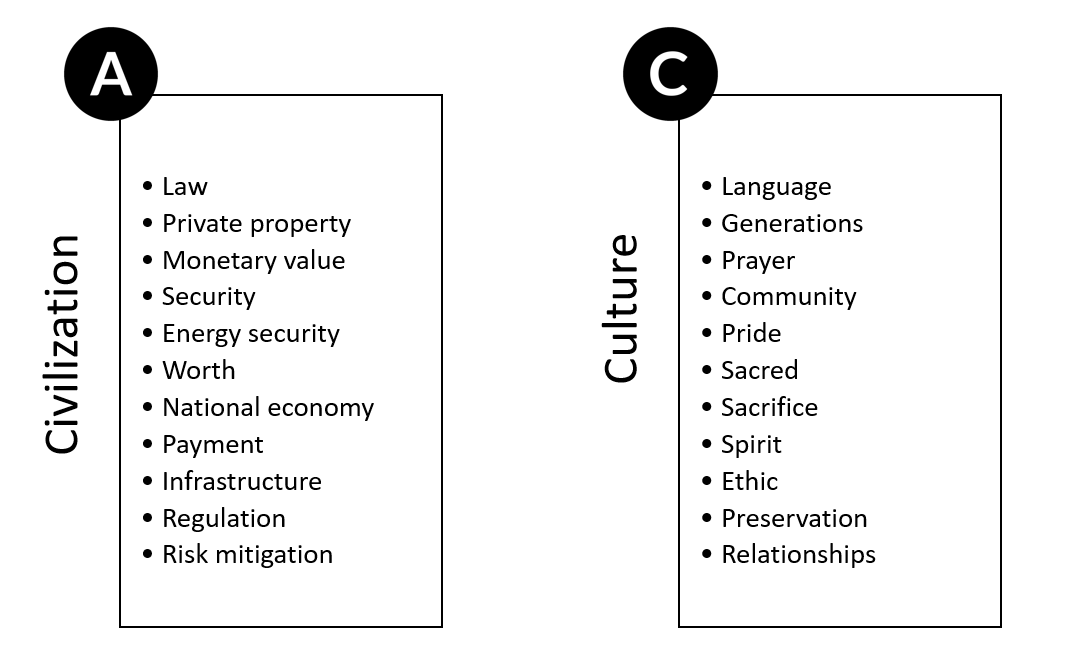
\includegraphics[width=10cm]{Figures/groupcontrast.png}
\caption{Key themes from Groups A and C in Analysis 2 (Chapter 4)}
\label{fig:figure1}
\end{figure}

Given the standpoint of the speakers, the contrast between A and C is not surprising. While those in Group C are speaking as members of civil society or communities, Group A is made up largely of individuals acting in occupational roles, representing state institutions or corporations. Arguably, speakers in Group A are compelled to employ relatively narrow discourses or `talking points'. In this sense, the two groups are playing entirely different language games. 

Between A and C, is Group B, where pipeline opponents invoke notions of trust, fairness, and inequality. Speakers in Group B speak out against an oppressive justice system, corporate power, exclusion, and economic inequality. Group B offers counter discourses to Group A. Speakers are engaging in critical commentary of broader social and institutional structures. In other words, they are expressing malaise with the prevailing civilization. While there are references to cultural groups, these are most often in the context of broken promises and perceived bias; these are not affirmative expressions of cultural identity in the same way as Group C. In terms of cultural discourse, the three groups can be summarized as follows: 

\begin{itemize}
  \item \textbf{Group A} consists of acultural statements representing social/institutional structures.
  \item \textbf{Group B} consists of statements made in reactive opposition to Group A, or challenging the legitimacy of A.
  \item \textbf{Group C} consists of affirmative assertions of culture.
\end{itemize} 
  
Group B is playing a language game compatible with A (call it a language game of civilization or institutions). At the same time, however, speakers are making some cultural assertions related to their identities and values. In this sense, Group B is also a pivot away from the language game of A. The malaise expressed in Group B can be understood as a move towards cultural assertions observed in Group C. Cultural discourse is thus conceived as a turning away from the language games of institutional power structures. Lost of trust and legitimacy with respect to the wider society is restored by a turn toward shared identity and experience.  
 
A similar grouping can be considered in Chapter 5. Here, we note how nonverbal communication operates differently depending on the level of discourse. Nonverbal expressions and their cognitive underpinnings are tied up with a given language game. Cultural language games are often accompanied by expressions of pride, confidence, and empowerment. Like Group C in Analysis 2, the cultural-level statements in Analysis 3 are affirmative. The socio-economic statements, on the other hand, are made in resistance. Rather than affirmative stances, speakers are speaking from a position of vulnerability and even fear. This contrast suggests that the language games operate beyond the content of verbal expressions, and are bound up with cognition and behavior.    
 
Following the argument that cultural language games are distinct from those of civilization, we can consider the aims for discourse analysis. One such aim might be to point out and resist departures from culture in the name of civilization or material progress, where ``civilization'' and ``progress'' do not refer to some more advanced state, but to prevailing ideas or myths of modern societies \citep[e.g.][]{Pollard1971a, Bowden2011a}. This aim entails the preservation of culture against onslaughts in the name of social or economic progress. From a critical standpoint, one could counter this aim, claiming it is suggestive of romantic conservatism or is reactionary to progress. However, it is possible that critical, anti-oppression, emancipatory frameworks are consistent with, perhaps even strengthened by, the idea cultural preservation. Similarly, the notion of an affirmative cultural identity as empowering could be the basis of autonomy in the face of oppression. 

Making a distinction between culture and civilization does not imply that we replace nuance and historical particularity with what could be criticised as a sweeping, Spenglerian narrative. It does, however, imply more measured use of the term `culture'. It is possible that this distinction enriches our understanding of what human cultures are and what they are not. In the contemporary context of global migrations and mass communication, contrasts between discourses of culture and those of civilization could be made; the former being expressive, symbolic, and related to dwelling in a particular time and place; the latter placeless, material, and uprooted from shared meaning. This distinction would challenge the notion of interculturality as internationalization of trade, science, technology, and socioeconomic structures \citep[see][5]{Mall2000a}. Accordingly, in societies often described as `multicultural', much of the discourse of business, media, politics, and science might be more aptly characterized as acultural cosmopolitanism. 

\subsection{Language Games \& Organicism}

The notion of language games emphasizes the diversity of human experiences, world pictures, and ways of using language. If communication is made up of sub-systems or ``games'' then one could raise the question of how mutual understanding is even possible. Underlying the diversity of language games, however, is a shared human form of life. Arguably, our shared life-form is itself constrained by the pre-linguistic, natural world. The relation to the natural world, as expressed in cultural language games, is not one of strict correspondence or \textit{a priori} understanding but is built upon layers of analogy and metaphor. The organic nature of human language has implications for the idea and aims of the ecological level of discourse analysis as well as how scientific statements can be approached in a discourse analytic framework (implications which will be elaborated in a subsequent section).

In a metaphorical sense, culture stands in relation to nature as an organic form. Organic form has a number of overlapping connotations related to artistic expression, human culture, and biological life. As a literary term, it is associated with Coleridge's idea of ``unity in multeity.'' Goethe's morphology is also ``a science of organic forms'' which aims to discover ``unity in the vast diversity of plants and animals'' \citep[xvi]{Miller2009a}. In \textit{Decline of the West}, \cite{Spengler1965a} refers to cultures through world history as the ``waxing and waning of organic forms'' (17-18).

The idea of language as organic form is embedded in the notion of language games. In later writings, Wittgenstein sees language as consisting of ``an inorganic part, the handling of signs'' and ``an organic part...understanding these signs, meaning them, interpreting them, thinking'' (BB, p. 4). The Investigations further develops the organic notion of language: ``In use it is alive'' (PI, \S 432). It is dynamic, with parts dying off and others ``coming into existence'' (PI, \S 23).

The connection between culture and organic form is based on a certain interpretation of \textit{forms of life}. Underlying the diversity of cultural language games is a shared human form of life. There are several interpretations of the meaning of this concept including social, cultural, behavioural, and biological accounts. Forms of life can be understood as patterns and regularities ``in the fabric of human existence on earth'' \citep[132]{Pitkin1985a}. \cite*{Sluga2011a} describes Wittgenstein's philosophy as a kind of naturalism where ``forms of life, worldviews, and language games are ultimately constrained by the nature of the world'' (12-13). However, one could also argue that these constraints are more anthropological than biological. \cite{Keith2012a}, for instance, claims Wittgenstein's position is one where there are no natural constraints on what can count as truth ``unless they are constraints on our shared forms of living'' (487). \cite{Cavell2013a} allows for both perspectives, suggesting forms of life be seen as a relativistic ``sense of agreement'' as well as in a more fixed, biological sense (41-42). It follows that, our shared human lifeform is itself constrained by the prelinguistic, natural world. This relation to the natural world is not one of strict correspondence or a priori understanding but is built upon layers of analogy and metaphor. 

If forms of life are indeed constrained by the nature of the world, then there would be a unifying ``system of reference'' common to all human cultures (PI, \S 206). What is common to all cultures might be activities of eating, drinking, or speaking a language (PI, \S 25). Science and technology might also reflect transcultural, universal truths. Relativistic interpretations of forms of life counter any suggestion of universalism. However, it is important to consider that Wittgenstein does not deny the possibility of a single or universal form of life. Sluga (2011) discusses a ``single form of life'' as a homogenized, unified language game and claims that, according to Wittgenstein, such a life-form would be ``impoverished and almost sub-human'' (61). Insofar as Wittgenstein invokes this possibility, it seems to have been a source of deep pessimism concerning the age in which he lived. Broadly speaking, this pessimism seems directed toward the scientism, positivism, and materialism he sees as characteristic of modern thought. As the antithesis of the organic diversity of language games and forms of life, Wittgenstein is critical of the homogenizing force of modern science and technology:

\begin{quote}
Perhaps science and industry, having caused infinite misery in the process, will unite the world\textemdash I mean condense it into a single unit, though one in which peace is the last thing that will find a home. (CV, 63)  
\end{quote}

\begin{quote}
Science: enrichment \& impoverishment. The one method elbows all others aside. Compared with this they all seem paltry, preliminary stages at best.  (CV, 70)  
\end{quote}

\begin{quote}
The use of the word ``science'' for ``everything that can be said without nonsense'' already betrays this overestimation. For this amounts in reality to dividing utterances into two classes: good \& bad; \& the danger is already there. It is similar to dividing all animals, plants \& rocks into the useful \& the harmful. (CV, 71) 
\end{quote}

These statements do not imply that Wittgenstein was somehow against science. Rather, they are a critique of the notion that the methods and aims of science can (or should) be applied across the range of human thought and forms of life \citep{Read2016}. This criticism is based on a naturalism that seeks complexity and interconnection while resisting reductionism. Similarly, an intercultural discourse analysis might aim to critique reductionism and scientism. This point returns to a previous question of how scientific statements are accounted for in a multilevel discourse framework. Critical analysis of natural scientific discourse is not directed at science \textit{per se}; rather, the ideology of scientism is what is problematic from an intercultural communication standpoint. 

Organic form functions as an ontological metaphor \cite[25]{Lakoff1980a}, whereby our experience of lifeforms is the basis for understanding. For example, we can consider how Coleridge identified organicism in properties of the plant. These properties are explained as five principles by \citeauthor{Abrams1953a} (\citeyear[170-75]{Abrams1953a}). These principles (and the organic form metaphor) might be extended to human cultures as follows:

\begin{enumerate}[i.]
  \item \textit{The whole is prior to the parts}. Although cultures are made up of a multitude of parts (people, groups, practices, beliefs, etc.), the culture itself is irreducible and cannot be understood through individual components separate from the whole.
  \item \textit{The process of growth is conveyed}. Growth as ``the first power'' of living things is manifest in cultures. Human cultures are dynamic, undergoing growth, death, and evolution. 
  \item \textit{Diverse elements are assimilated into the whole}. Human cultures form as individuals and groups combine. The individual elements metamorphize into the whole.
  \item \textit{Form and growth is directed from within}. Cultures evolve spontaneously from within. By contrast, mechanical forms arise through an externally imposed structure.
  \item \textit{Unity in multeity}. In human cultures, a complex interdependency of parts forms a whole. The whole and parts are interdependent, with the whole (culture) relying on the components and vice versa. 
\end{enumerate}

The organic form metaphor for cultures is consistent with an antireductionist and holistic approach that, in the opening of this chapter, was stated as necessary for intercultural research. Nature, as the organic wellspring for cultures, consists of complex forms of life. It follows that culturally imbued statements themselves evoke this complexity which, while expressed through cultural practices, may not be articulated or rationalized.	

\section{Unsurveyability \& Cognitive Bias}
 
The previous discussion deals with philosophical concepts that, one could argue, do not clearly apply to the everyday practice of intercultural communication. In order to sketch out how these concepts might be applied, this section discusses the idea of unsurveyability in terms of cognitive bias. The argument is that, in the three analyses of environmental communication, there is a tendency to move away from the cultural context, towards more defined, measurable ways of framing the topic. This tendency can be seen as a natural cognitive response in the face of complex, unsurveyable phenomena.   

Culture and communication are what \cite*{Sluga2011a} terms ``hyper-complexities'' (146). At most, we can only obtain partial understandings of the language games and multilevel interactions that constitute a given discourse. In the face of complexity, it is natural to reduce and categorize. For instance, from the some 7.5 million colours discernable by the human eye, we assign categories like red, glue, green, etc. \citep[889]{Hinner2017a}. This categorization prevents chaos in the realm of human perception and cognition, allowing us to simplify phenomena to manageable proportions. However, this inherent tendency to simplify and categorize can lead to bias. Cognitive bias arises from heuristics and mental shortcuts in the face of uncertainty and complexity \citep{Kahneman2002a}. Bias may thus be understood as information-processing shortcuts in the face of uncertainty \citep{Tversky1974a} or noisy information \citep{Hilbert2012a}, together with the human brain's limited capacity to process that information \citep{Simon1955a}.

Culture is a hyper-complexity with layers of metaphor and meaning inherent in behaviors and utterances. For example, in the corpus examples we see how cultural statements evoke connotative, contextual, and figurative meanings \citep{Klopf1998a}. Yet, in the face of this complexity it is common for people to frame discourse in narrower, more literal, and more sharply defined terms. This framing often negates the cultural context. This turn away from complexity might be described as a \textit{surveyablity bias} whereby, in the face of complex unsurveyable phenomena, people frame the issue according to a limited perspective. Like other biases, the surveyability bias can be viewed as a mental shortcut in the face of complexity. Unlike the conventional notion of bias as prejudice, surveyability bias is a departure from cultural meanings altogether. For instance, in the GM seed debate which (as we note in Analysis 1) is highly cultural, there is a narrowing of the discourse to issues of safety and efficiency. Due to the complexity of cultural schemas, there is an inherent tendency to perceive and interpret that which is part of the common system of reference while neglecting the culturally variant frame. 

This notion of bias changes the way we might look at intercultural misunderstandings. In intercultural encounters, it is common to refer to cultural bias, which is a preference for one cultural group over another \citep{Yingst2011a}. Similarly, intercultural conflict is conventionally seen as a perceived incompatibility between different cultural communities \citep{TingToomeyS}. However, many conflicts between groups are not intercultural. Likewise, communication from people from different cultural communities often does not necessarily lead to misunderstanding. Rather than looking at how conflict arises from differences among cultural groups, it may be more appropriate to view conflict and misunderstanding in terms of whether the cultural dynamics are even being taken into account. In modern, pluralistic societies people do not express their cultural identities at every turn, at least in the public sphere. In terms of the familiar culture as an iceberg metaphor \citep{Hall1973a,Hall1976a}, daily lives are conducted at the surface. As opposed to viewing communicative interactions as encounters between different cultures, we can consider how culture emerges to the surface at different points.	 

As discussed, human communication can be viewed as an amalgam of different language games. Different language games imply different rules that guide the speech and behaviour; different meanings of words within a system of reference; different human needs that the language game fulfils; and actions to which it corresponds. Along these lines, communicative misunderstandings result from incompatible language games both within and between cultures \citep[10]{Frayne2017a}. More specifically, misunderstandings result when interactants are unaware that entirely different language games are being played. Surveyability bias is precisely this lack of awareness that a language game is indeed cultural.

\subsection{Family Resemblances \& Surveyability Bias}

Like other biases, the surveyability bias is unavoidable and part of our cognitive make up. However, there are certain ways of thinking that can counteract this bias. The remedy for surveyability bias is to obtain a more synoptic view or surveyable representation of complex phenomana like cultures. This ``consists in seeing connections'' (PI, \S 122). Wittgenstein claimed ``our grammar lacks surveyability'' (PI, \S 122), implying the complexity of natural language is such that we cannot grasp it in its entirety. Even though we cannot represent language as a whole system, we can look at its multiple uses. Taken together, these particular uses will reveal relations and patterns of similarities that can be characterized as ``family resemblances'' (PI, \S 67). Family resemblance is a way to confront the challenge of understanding cultures, their language games, and the set of relations that exist within and between them.

Rather than serving as an entirely new idea, family resemblance gives new expression to what is already implied in much intercultural research, particularly comparative approaches. Like language games, cultures can be characterized as having both intercultural and intracultural family resemblances. In other words, when we associate people or things with a culture X, we are saying there is ``no one thing in common which makes us use the same word for all'' but that they are related ``in many different ways'' through ``a complicated network of similarities overlapping and criss-crossing'' (PI, \S 65, 66). In the same way, different cultures form a complicated network. Amid the plurality of cultures and language games, interconnectedness makes communication and understanding possible. Family resemblance need not imply strict biological inheritance. By contrast, it is a general picture that forms when any number of individuals/entities are grouped together by a set of characteristics that may not be common to all \citep{Ginzburg2004a}. Networks of biological descent, family bonds, ethnicities, races and nations might be an important part of this grouping. However, there are other important factors such as citizenship, geography, or shared history \citep{Sluga2011a}. Establishing family resemblance is a matter of sketching out the multiple relationships. The task for intercultural research could be to form a ``genealogy of concepts'' within and between cultures \citep{Canfield1993a}. In this, metaphor and analogy are central since it is in this way that cultures relate back to a shared human form of life.

In Analysis 1, we see examples of the role of metaphor in maintaining agreement and mutual understanding among anti-GM critics. In the keywords, concordances, and the ``Maize Manifesto'' excerpt, there is a bidirectional metaphor between culture and nature. In other words, there is an implicitly understood reciprocal relationship between human culture and nature. The diversity and complexity of each is understood in terms of the other. The function of this biocultural metaphor is to capture the internal complexity of the topic at hand and frame the issue holistically. Thus, even if GM critics do not share a common culture, there is a common set of concepts that create meaning and reconciles worldviews cross-culturally.  

The pipeline debate (Analysis 2) also has a strong cultural element, particularly with respect to the indigenous groups. Here, we see the expression of cultural values, or a set of deeply held beliefs among a cultural group \citep[95]{Martin2010a}. However, non-indigenous voices are also present. We see family resemblances between these different worldviews with respect to, for instance, the spiritual dimensions of nature.

In the three analyses we observe that disagreement and misunderstanding arise from the inability to make connections between worldviews and experiences, not necessarily from cultural differences. At times the source of disagreement is ontological, insofar as it related to underlying assumptions about the nature of reality and categories of being. At other times, the disagreement could best be traced to cognitive factors, in the sense that it goes beyond ontological thinking to also encompass values and emotions \citep[114]{Palmer1996}. 

What we observe from the three analyses is that environmental issues bring clashes and contrasts in worldviews to the forefront. Of course, environmental issues are not unique in this regard. However, there are few topics that expose, like environmental issues do, that worldviews differ even with respect to the human understanding of the natural world. In other words, whereas we might often attribute differing worldviews to subjective interpretations, environmental debates remind us that worldviews operate at the deeper layer of the ontological and epistemological approaches to nature itself.

To summarize, Wittgenstein's thought can help us conceptualize the relation between culture and language. Concepts of language games and unsurveyability allow us to grasp the challenges of understanding one another. We can consider the notion of family resemblance as a framework for overcoming these challenges. For intercultural research, we might also consider the idea that there are discourses of culture and civilization. Implicit in this latter point is that discourses of culture are rich and meaningful in ways that those of civilization are not. This discussion leads to the question of the conditions under which mutually intelligible cultural language games are made possible. To address this, we turn to the idea of the public sphere.

\section{Plurality \& the Public Sphere}

Concepts form Wittgenstein's philosophy help us integrate culture, communication, and language. One potential drawback of these concepts, however, is that have relatively little to say about the political sphere or the socio-economic level of analysis. To account for this, another point of departure for a non-essentialized conception of intercultural communication are Arendt's notions of plurality and the public sphere. Arendt's thought can be placed within the phenomenological and hermeneutic traditions; the former rooted in direct engagement with the world and the latter concerned with interpretation of meaning. Since it emphasizes language and social interaction, hermeneutic phenomenology is especially relevant to communication theory \citep[49]{Littlejohn2011a}. Its emphasis on language as a conduit of meaning also makes this tradition relevant to intercultural understanding.

Plurality is based on the premise that ``nobody is ever the same as anyone else who ever lived, lives, or will live'' \citep[78]{Arendt1958a}. A plurality of perspectives emerges from the radical finitude of each human having been born into a unique place and time. However, this is not an individualized or atomized existence. Our being-in-the-world is characterized by a ``web'' of human relationships within which we experience this plurality \citep[175]{Arendt1958a}. This plurality ``is a blessing'' since the perspective of the others puts one's own perspective ``in relation with the world'' \citep[443]{Gambetti2005}. In the condition of plurality, humans come together and deliberate through the public sphere. The public sphere has the capacity to unite humans in meaningful action while preserving their freedom and plurality. 

Arendt's notions of plurality and the public sphere are pertinent to environmental communication. As the three prior analyses highlight, ecological issues are debated in diverse societies across multiple, unbounded geographic scales. These discourses take place in similarly unbounded intercultural communicative spaces that can be described as the ``global public sphere'' \citep{Volkmer2014}. Deliberations about environmental issues constitute what Arendt described as the two dimensions of the public sphere: (i) the \textit{space of appearance} and (ii) the \textit{common world} \citep{DEntreves2018a}. In an age when political processes are privatized \citep{Wolin2008}; civic institutions eroded \citep[see][]{Putnam1995}; and digital communication commodified \citep{Fuchs2009a}, the physical environment becomes a \textit{space of appearance} for authentic and free deliberation. Moreover, since environmental issues speak to the basic necessities of life (water, food, air, etc.) they are crosscutting themes in pluralistic societies. Amid all the planet's cultural diversity, the earth itself is a basis for common action. The environment is the ground upon which the \textit{common world} of human artifacts and institutions is established.

Arendt's public sphere theory points to the importance of maintaining conditions for free and open discourse. A challenge for pluralistic societies is not only misunderstandings and conflicts that arise within the public sphere due to, for instance, intercultural differences. The challenge also lies in creating and maintaining spaces where free and open communication can even take place. The very spaces that allow for public deliberation are often influenced and thwarted by dominant groups and ideologies in society. Structural and institutional forces can undermine the open and pluralistic character of public spaces. In modern capitalism, these forces often stem from economic interests or the harnessing of political institutions to advance private ends. If we take Arendt's notion of the public sphere as a prerequisite for intercultural communication, then crucial questions for ICC research relate to the political and economic conditions that impede authentic communication from taking place.

Another important question for ICC is the role and influence of scientific discourses in the public sphere. Of course, in the context of environmental issues, there is an indisputable role for scientific discourse to play. However, science is embedded in cultural or political contexts. There is thus a case for viewing science from a humanistic and critical standpoint. \cite*{Peet2011}, for instance, point out that scientific discourse can ``exclude or marginalize'' and be ``partial, reductionist, and instrumental in achieving and maintaining political control over nature'' (31). The specialized characteristic of scientific practice poses a challenge to open and free deliberation in the public sphere since, in many cases, the sciences employ a language of symbols that ``in no way can be translated back into speech'' \citep[4]{Arendt1958a}. There is a role for intercultural communication in understanding these issues and, building on recent research spanning ICC and Science and Technology Studies \citep[e.g.][]{Reyes-Galindo2017a}, it is important to consider communicative issues that arise when science crosses social and cultural boundaries.  

Arendt's notion of the \textit{common world} highlights that establishing shared meaning is imperative for addressing ecological issues. It is within the public sphere\textemdash through language and communication\textemdash that we establish and maintain shared meaning. Meaning is created through authentic discourse that is not ``empty'' or used to ``veil intentions'' but which discloses realities \citep[200]{Arendt1958a}. Arendt highlights the importance of paying close attention to communication in the public sphere and being wary of decisions made in the name of efficiency and technological advancement. 

\begin{quote}
There is no reason to doubt our present ability to destroy all organic life on earth...it is a political question of the first order and therefore can hardly be left to the decision of professional scientists or professional politicians. \citep[3]{Arendt1958a} 
\end{quote}

Arendt wrote this in the wake of WWII, as the Cold War and nuclear proliferation were gaining momentum. For Arendt, the crisis of modernity was a symptom of alienation and loss of meaning and identity. So too can today's ecological crisis be seen as ``earth alienation'' and an accompanying loss of meaning. Of course, there are aspects of Arendt's thought that are problematic from an intercultural standpoint. Whereas Arendt returned to the ancient Greek \textit{polis} to rediscover fragments of lost meaning, an intercultural approach might also look to other cultural traditions. Nonetheless, the core ideas of the public sphere and the role of communication in creating shared meaning can be part of a normative framework for both intercultural and environmental communication.

\section{Redefining the Levels of Discourse}

This dissertation seeks to re-frame how human communication about the environment is analyzed and interpreted. To this end, concepts introduced above can help one understand, evaluate, and interpret language and communication. The ideas of Arendt and Wittgenstein can be employed to guide and orient research, either implicitly or explicitly.

Arendt's notion of the public sphere can be held up as an aim for intercultural discourse. Instances where this aim is undermined can be critically assessed. Scientific and technical language can be analyzed in light of plurality and the public sphere. Based on Arendt's concepts of alienation and meaning, analysis might seek to identify manifestations of ``earth alienation'' and draw out cultural meanings associated with the natural world. Arendt's thinking also informs the political and social critique that are central to discourse analysis.

Wittgenstein's notion of language games serves to highlight the diversity of language and communication. There is an implicit relation between ecology, language, and culture that is based upon the notion of organicism in Wittgenstein's thought. Wittgenstein might also be evoked to understand a type intercultural misunderstanding which results from incompatible language games, examples of which we saw at several points in the corpus analyses. Finally, the unsurveyability of human cultures forms a basis for critiques of reductive thinking and evasion of cultural context.

The opening chapter of this dissertation refers to the need for a conceptual or normative framework for ICC and environmental sustainability. Principles for such a framework are now outlined as:

\begin{itemize}
  \item Preservation of plurality, both cultural and ecological
  \item Maintaining conditions for shared meaning in the public sphere
  \item Appreciation for the complex, unsurveyable nature of human cultures and languages
\end{itemize}

Of course, the concepts outlined here are broad and could be applied and interpreted in many ways. To operationalize these concepts in ICC scholarship, we can consider what these concepts mean in the context of the multilevel analysis. The following section revisits multilevel analysis as a framework for organizing and integrating various high level concepts. Multilevel principles can thus serve as a segue between theory and methods.  

In light of the conceptual principles, we can revisit the four levels of discourse first introduced in Chapter 2. Previously, we looked at the levels in terms of \textit{data} and \textit{analysis}. To further develop these notions with the conceptual framework of this chapter, we draw from \cite*{Blommaert2005a} to explain two more foundational components of each level:   

\begin{enumerate}[i.]
  \item \textit{Concept of discourse} 

Different levels entail different ways of approaching the notions discourse and communication. Thus, the \textit{concept of discourse} aims to outline what discourse is at a given level. This includes what modes of semiosis are employed and how communication stands in relation to the world. These questions also concern what objects of communication are analyzed (speech, body language, etc).

  \item \textit{Aims of analysis} 
  
Here the questions concern the themes/topics that are covered at each level as well as the normative framework against which discourse is analyzed. For example, principles of equality and justice might inform the critical analysis of socioeconomic discourse. By contrast, ecological analysis might be motivated by different evaluative principles, such as species conservation. The cultural level might aim for principles of plurality and preservation of identity.     
\end{enumerate}

From the corpus analyses of previous chapters, we conclude that different levels of discourse often constitute entirely different language games. Thus, we need to distinguish levels not only from the semantic contents of the communication (i.e. data), but the underlying assumptions about communication itself.
 
\subsection{Ecological Level}

\textbf{Concept of Ecological Discourse}

The environmental crisis calls upon us to extended the focus of discourse analysis from social/political to ecological issues. Some researchers have begun this task. Notably, \cite*{Stibbe2014b} outlines an ecolinguistic approach to CDA focused on ``discourses that have (or potentially have) a significant impact not only on how people treat other people, but also on how they treat the larger ecological systems that life depends on'' (118). Ecological CDA inherits many of the premises and aims of social-political variants. The latter is concerned with the way discourse constructs ideologies and worldviews that create social power and hegemony (humans vis-\`a-vis humans) and the former addresses how language-use as a social practice has ecological impacts (humans vis-\`a-vis other species). However, ecological questions challenge some concepts and aims underlying conventional discourse analysis.

In extending analysis from social to ecological questions, the concept of discourse has generally remained consistent to that in conventional CDA. \cite*{Stibbe2014b} introduces ecological discourse as an approach to ecolinguistics with examples that are primarily text-based including advertisements, newspaper reports, industry journals as well as literatures, stories, poetry (122-124). Along the same lines, \cite*{Muhlhausler2006b} explicitly define environmental discourse as linguistic devices, citing examples of product slogans, public and commercial radio/television, corporate and political communications, vernacular used in protest movements, environmental impact assessments, and literature. 

Although these examples cover a wide range, \cite*{Jasanoff2004a} points out two important aspects that remain overlooked in environmental discourse frameworks. First, formal discourses of policy and law are often given analytic priority over vernacular traditions and, second, the discourse framework ``downplays the role of material instruments and that of human interpretive faculties other than language'' (36). What is needed, therefore, is a notion of discourse that more explicitly accounts for the vernacular, material, and nonlinguistic.

Discourse that engages multiple semiotic viewpoints implies more diverse objects of analysis than conventional CDA. For example, ecological discourse encompasses sociocultural as well as geographic space. Whereas conventional CDA analyzes text, speech and multimodal communication, objects of ecological discourse analysis may include scientific models and maps \citep[44-45]{Jasanoff2004a}, the built environment \citep{Rapoport1994}, landscapes and, ultimately, direct experience of nature as semiosis. 

An appropriate broadening of the concept of discourse can be found in ecosemiotic and ecolinguistic literature. Ecolinguistics\textemdash by taking into account both the social and ecological context of language\textemdash does, in fact, emphasize vernacular and ordinary language. Moreover, the material and nonlinguistic aspects of discourse are part of semiotics. Just as CDA can draw from nonlinguistic semiotics by examining several modes of signification and meaning, other branches of semiotics can be considered from the nonhuman world. Particularly appropriate is the emerging field of ecosemiotics, since it studies signs and signification as part of both the human and nonhuman worlds \citep{Noth1998a, Maran2014a}. 

Discourse has conventionally been defined in anthropocentric terms such as that which ``sets us apart from other species'' \citep[4]{Blommaert2005a}, an ecosemiotic view suggests discourse is in dialectic relation to the human and nonhuman worlds. Ecosemiotics is based on Jakob von Uexk\"ull's (\citeyear{VonUexkull1982}) concept of the intersubjective \textit{Umwelt} as well as more recent approaches that synthesize discursive and prediscursive meanings \citep{Kull1999a, Sebeok2001a, Maran2007a}. This implies a synthesis of cultural semiotics (where the point of view remains within the limits of human language and culture) and biosemiotics (which is interested in sign relations between living organisms and their environment) \citep[279]{Maran2007a}. Methodologically, this approach engages multiple semiotic viewpoints and is rooted in the phenomenological lifeworld of humans and other organisms \citep{Buchanan2008a}.

One implication of an ecosemiotic view concerns the relation between discourse and the environment. The question of how discourse constructs social reality (and vice versa) has long been central to CDA. Many in the social sciences argue that language both shapes, and is shaped by, social reality. In light of the Anthropocene and the extent to which human beings can alter planetary life, we can also consider how human communication shapes, and is shaped by, the natural world. In other words, the human and nonhuman worlds are co-constructed through discourse.

\textbf{Aims of Ecological Analysis}

As \cite*{Stibbe2014b} points out, the traditional aims of CDA are not necessarily sufficient in an ecological context: ``freedom and democracy do not automatically lead to sustainable levels of consumption, and peace in a society that exceeds environmental limits will be short lived'' (120). Indeed, the human world is imbued with unique capacities for justice, reciprocity, and forgiveness, but when ``acting into nature'' the consequences may be unpredictable and irreversible \citep[59]{Arendt1958a}. One could also question whether theories and methodologies underlying CDA can be extended to scientific arguments that are central to ecology, particularly given the wide methodological gulf between CDA (which is deliberately not politically neutral) and the natural sciences (which aim to be value-free and objective). Furthermore, a turn to ecological themes invokes longstanding conceptual debates regarding the relation between `nature' and humanity, as well as the normative basis for an environmental ethic.

To establish aims of ecological discourse analysis, we can further consider the dialectical relation between the human and nonhuman worlds. Experience with nature and other species shapes our conceptual understanding and, ultimately, human culture. Conversely, through discourse, human culture transforms and constitutes the environment. Conceptual interpretations of the environment result in symbolic categorizations in human language which, in turn, frame physical (and even biochemical) manipulations of the environment ``leading to the culturization of nature,'' or what is often called ``second nature'' \citep[45]{Maran2014a}. 

Analysis of ecological discourse seeks to point out when this dialectic, communicative relation with nature is disrupted or is otherwise harmful to the biosphere. Critique may be directed towards instances where symbolic categorizations and manipulations of the environment are not conducive to ecological flourishing. Such critique draws on the next analytical level (cultural discourse analysis), since we are interested in how relations to the environment are culturally framed. As argued in the next section, human cultures mediate cultural semiosis (in the human world) and natural semiosis. However, in modern societies natural semiosis becomes eclipsed by human artifacts, technologies, and symbols. This results in humans becoming ``prisoners of the cultural semiotic'' (\citealt{Stibbe2014b} 105; citing \citealt{Halliday1978a}). This closure is characteristic of modern technological existence where human utterances are ``elicited, directly, by humanmade signs'' and ``the larger, more-than-human life-world is no longer a part of the semiotic'' \citep[101]{Abram1997a}. 

Discourse uprooted from ecological context leads to ruptures in the human relation to the earth. Although ecological analysis seeks to critique such uprooting, the ultimate aim of ecological level analysis is not merely to critique communication; rather, the aim is to renew it. Discourse is not merely an object of analysis but language itself is a basis for ecological flourishing. Establishing an authentic human relation to the earth entails ``breathing life'' into language \citep[10]{Clingerman2014a}. Human cultural traditions are imbued with meanings and symbols expressing the human relationship to nature. Beyond critique of ecological destructive discourses, the aim is to understand and preserve those traditions that value and conserve nature.

To summarize, the ecological level challenges us to expand the very notion of communication from the human to more-than-human realms. Natural processes influence human communication and vice-versa. This is to say there is a dialectic relation between nature and culture. An aim of analysis of human communication (i.e. discourse analysis) is to be aware of this dialectic and be critical of ways in which human language and semiosis engenders ecological destruction. 

\subsection{Cultural Level}

\textbf{Concept of Cultural Discourse}

As discussed in previous sections, we can distinguish \textit{cultural} discourse from other levels of analysis. Specifically, a distinction between the cultural and socioeconomic levels can be made. 

While acknowledging that culture is inescapable and ever-present, we can also view it on a continuum, present or absent at various times and to varying degrees. We might also consider that there is much to communication and behaviour that constitutes human culture (i.e. shared by all humans) but does not differentiate one culture from another. Returning to Wittgenstein's terms, there are human forms of life where cultural differences are irrelevant or negligible. These forms of life are what Wittgenstein refers to as ``the common behaviour of [hum]mankind'' and ``the system of reference'' that makes communication possible across languages and cultures (PI, \S 206). Here, to refer back to the ecological level, we point out how the natural world could itself constitute that system of reference.

In addition to a common system of reference, Wittgenstein emphasizes the diversity of human experiences, world pictures, and ways of using language. Although cultures stem from a shared human form of life, they branch out in diverse ways. The cultural level of discourse analysis seeks to understand how this diversity is reflected in human communication. 

The connection between culture and discourses is apparent if the latter are seen as ``culturally infiltrated'' language games \citep[5]{Shi-xu2005a}. In intercultural situations, these games are more likely to be divergent, opposing, and disorienting, thus leading to misunderstandings. It follows that discourse analysis is a useful tool for describing these games, their rules, internal logic, the human needs they serve, etc.  

\textbf{Aims of Cultural Analysis}

A cultural mode of analysis might focus on different types of discourse. In CDA, discursive objects are generally forms of speech or text in larger units than single words and sentences. Critical analysis has also been extended to nonlinguistic or multimodal communication and social semiotics, including gestures, film, media, art, sound, typography, and questions of colour \citep[2, 15]{Wodak2009}. Whereas CDA often concerns textual and discursive artefacts, cultural analysis is more likely to also account for the actual practice of metalinguistic, nonverbal communication and behaviours.	

One aim of cultural discourse analysis is to critique the tendency to look at things too narrowly and decontextualize subject matter. Taking discourse as an object of analysis is to separate it (at least to a degree) from the practices and nonlinguistic forms of life into which language games are interwoven. To be sure, ethnography of communication \citep{Hymes1972a} as well as more the recent frameworks of \cite{Blommaert2005a}, \cite{Shi-xu2005a} and others have done a great deal to bridge this separation \citep[see][for an overview]{Scollo2011a}. Nonetheless, the tendency to drift from deep, culturally embedded meaning and context is everpresent, as is the tendency to avoid consideration of nonlinguistic, nonverbal behaviors and expressions. It could be argued that with digital and internet communication, the distance between language and situated context is greater than ever. As a result, the form of life in which language games have their meaning might be overlooked so as to exacerbate misunderstandings. In response to these challenges, cultural discourse analysis can be a method of metacritique, where language is continuously referred back to its cultural context.

\subsection{Socio-Economic Level}

\textbf{Concept of Socio-Economic Discourse}

In explaining the notion of discourse inherent to CDA, \cite*{Jorgensen2002a} place critical discourse analysis on a continuum between two opposing positions. On one end, based on the theory of Laclau and Mouffe, is the view that discourse is fully constitutive of the social world. Accordingly, discourse is not only text and talk but ``discourse itself is material'' and ``entities such as the economy, infrastructure and institutions are also parts of discourse'' (19). On the opposing end, discourse is fully constituted by the world, that is, ``a mechanical reproduction of other social practices...fully determined by something else such as the economy'' (ibid). This latter view follows from Marxist structural-materialism. In this model, critical discourse analysis is between these opposites in dialectic relation. In other words, discourse shapes our social reality and is determined by it.

\textbf{Aims of Socio-Economic Analysis}

Objects of critique in CDA are political, economic, and social ideologies and structures that result in injustices or inequality based on class, race, gender, and other factors \citep[250]{VanDijk1993}. While these aims certainly apply to the multilevel analysis, focus is also placed on how socioeconomic factors relate to the preceding levels; namely, the ecological and cultural. For instance, in a multilevel framework, the task of critical social analysis can be focused on the social conditions for maintaining authentic intercultural discourse. Thus, returning to Arendt's notions introduced earlier, the socioeconomic level is concerned with conditions to maintain a free and open public sphere where authentic communication can take place.

The notion of authentic communication is where the relation between cultural and socioeconomic levels comes into focus. Communication problems arise from social-institutional factors that act as barriers to a public sphere where authentic dialogue can take place. As mentioned, the socioeconomic level is most closely related to critical theory and CDA. The notion of communication central to critical theory is influenced by Habermas' (\citeyear{Habermas1984a}) idea of reaching mutual understanding in ideal discursive conditions. In terms of communication theory, critical and cultural analysis combines critical-theoretical and phenomenological approaches, respectively. The aim is not to reconcile these two distinct theoretical traditions but to trace the concept of authentic dialogue as a common thread. 

\cite*{Craig1999a} notes how the ideal of dialogue is common between the critical-theoretic and phenomenological models of communication (148). In the phenomenological tradition, communication is the direct, authentic, and unmediated being-with others. The difference, as Craig states, is a gap between the communicative ideal and reality:

\begin{quote}
In a critical perspective, phenomenological dialogue represents an ideal form of communication, but one that existing socio-cultural conditions may render unlikely. \citep[148]{Craig1999a} 
\end{quote}

The concepts of ecological and cultural discourse (as explained in the previous sections) are closely related to what Craig refers to as phenomenological dialogue. Both emphasize deep, unmediated, authentic communication. It follows that barriers to dialogue are also barriers to ecological and cultural well-being. In everyday communication, however, conditions often preclude authentic discourse from taking place. The socioeconomic level of analysis, therefore, aims to uphold conditions for the preceding levels (ecological and cultural).  

In historical terms, much of what might be euphemistically described as intercultural encounters were, in fact, the loss of cultures in the face of pursuits of material gain and power. As examples, we could refer to imperialist histories and deliberate, state-sanctioned attempts to wipe out indigenous and minority cultures. Cultural loss may also result from more subtle failures to reciprocate or encounter `the other' on authentic terms. A more insidious example of present-day cultural loss is the precipitous decline of linguistic diversity \citep{Amano2014c}. To be sure, such cases could be described in cultural terms; for instance, as cultural hegemony \citep{JacksonLears1999a} or the majority vis-\`a-vis minorities \citep[4044]{Ashcroft2000a}. Yet, to refer to oppressive social relations as `cultural' seems to dilute the rich humanistic connotations of the term. To identify pursuits of material gain, oppressive state power, and unchecked globalization as departures from culture (as opposed to cultural encounters) would be compatible with a critical framework.

\subsection{Cognitive}

\textbf{Concept of Cognitive Discourse}

Recent approaches to cognitive science are more conducive to intercultural communication research than has traditionally been the case. For instance, there have been significant efforts to study the impact of culture on cognition \citep{Prinz2016b}. While traditional cognitive science may have been too narrowly conceived to deal with the subtleties of human communication and culture, alternate approaches such as embodied and 4E cognition (embodied, embedded, enactive, and extended) could be compatible with critical and non-reductive intercultural communication research. 

Discourse at the cognitive level can be seen as a reflection of individual mental processes, but also of shared cognition manifested as social structures and cultural beliefs. These structures and beliefs might be considered neurologically `wired' as cognitive frames. The relation between discourse and cognitive frames is significant for intercultural communication for several reasons. The idea implies that words derive their meanings in terms of a frame as opposed to in isolation. In other words, language does not correspond to the world directly but fits into to some frame. Moreover, these frames are variable between different people. Culture, in particular, plays an important role in the way cognitive framing develops \citep{Han2011a}. Of interest for intercultural communication, therefore, is how frames differ by culture; also, how individuals develop shared frames as well as how simple frames connect to form rich, textured meanings. In this light, intercultural misunderstanding might be considered as a misalignment of cognitive frames. Surveyability bias (introduced earlier in this Chapter) might also be understood as the substitution of one or more simpler frames in a communicative situation that is built on rich layers.

\textbf{Aims of Cognitive Analysis}

A cognitive approach to discourse can help us understand various reactions and responses to environmental issues and misunderstandings. For example, ecologically minded observers might decry how climate change skeptics ignore rational scientific evidence. Similarly, one might observe that such debates quickly become partisan or ideological. Cognitive analysis is crucial to understanding ideological divides over environmental (and other) issues. When ideologies are understood as systems of frames, certain words or phrases can activate an entire ideological system \citep[72]{Lakoff2010a}. Moreover, these frames are mostly unconscious, so changing an ideological frame is not easy. Facts and reason alone will not change one's belief system unless they fit within a system of frames \citep[73]{Lakoff2010a}. An aim of the cognitive level of analysis is to place statements within a system of mental frames and thereby consider not only \textit{what} people say, but \textit{why} they are saying it. 

This level of analysis looks at different expressions of cognitive bias in human communication. One way we can study the cultural and communicative dimensions of framing is through conceptual metaphor; that is, metaphor as a conceptual as opposed to linguistic phenomenon. The premise is that conceptual organization and, by consequence, thought itself is metaphorical \citep[303]{Evans2006a}. Metaphor is a mapping between conceptual frames. \cite{Lakoff1980a} showed how everyday language is full of these mappings which are unidirectional from a source domain to a target domain, often corresponding to the concrete and abstract concepts, respectively.

Conceptual metaphor can play an important role in socioeconomic analysis by, for instance, revealing negative biases against certain groups. For example, \cite*{VanDijk2015a} calls attention to ``wave'' metaphors to refer to immigrants. The wave metaphor, which is common in politics and media, invokes the ``fear of downing in so many immigrants'' and thus concretizes a concept in a way that is ``not social and politically innocent'' (75). Another metaphor used historically for political nefarious purposes is the nation state as a human body \citep{Musolff2012a}. The implication is that the state can ``fall ill'' due to ``disease spreading agents'' which as associated with social groups and individuals (303). 

The cultural level can also be informed by metaphor, by paying attention to those which are universal or culturally variable. Conceptual metaphors can be distinguished as primary or complex. Primary metaphors \citep{Grady1992, Grady2005a} are grounded in everyday experience and, with few exceptions, are similar across cultures. These are based on primitive concepts which are universal across languages and cultures. As \cite*{Lakoff2014a} states:  	 

\begin{quote}
Where the experiences are essentially the same across cultures, the metaphor mappings tend to be the same. They appear to be learned by experience via neural learning. (5) 
\end{quote}

To summarize, the cognitive level aims to go beyond surface layers of communication. By placing discourse in conceptual schema, cognitive analysis enhances our understanding of diverse perspectives. Along with cognitive linguistic concepts discussed in earlier chapters (implicature, ICMs, etc.), conceptual metaphor is another important aspect of discourse that can provide insights.

\subsection{Summary}

The preceding sections outline how each level entails different \textit{concepts of discourse} as well as different \textit{aims of analysis} (summary in Table 6.1). Together, the four levels of encompass a very broad scope. Yet, the scope is not too much broader than that of existing ICC research. The only truly new theme for ICC is that which is outlined in the ecological level. Cognition as well as critical/social analysis have long been integrated into ICC. The ecological level, however, adds a new dimension to the study of communication and cultures since, at this level, the realm of communication is expanded to encompass other species and nature as a whole. The ecological level challenges the aims, methods, and philosophical presuppositions of the field.

Of course, to separate the different levels is a simplification. In reality, there are no sharp boundaries between nature, culture, our social/economic lives, and cognition. Distinguishing the levels is merely a way to organize and understand complex, multilayered communication. While discourse analysis is a process of breaking communication down into the separate levels, it also entails uniting the various dimensions of communication into a whole. Ideally, the process leads to greater understanding without decontextualizing communication as it occurs in the \textit{Lebenswelt}.

\begin{table}[h]
\centering
\begin{footnotesize}
\def\arraystretch{1.5}% 
\begin{tabular}{| P{3cm} | P{4cm} | P{4cm} | }  
 \hline
\textbf{Level} & \textbf{Concept of Discourse} & \textbf{Aims of Analysis} \\
 \hline
\textbf{Ecological} & Semiosis in a more-than-human world; Dialectic relation between discourse and nature (discourse constitutes nature and is constituted by nature) & Critique anthropocentric/ environmentally destructive communication; call attention to symbols and meanings that preserve nature \\
 \hline
\textbf{Cultural} & Symbolic meanings, cultural commentary; 'culturally infiltrated' language games; metaphor of organic form; forms of life & Critique of decontextualization, uprootedness, loss of languages and cultural identities \\
 \hline
\textbf{Socio-Economic} & Discourse as power and hegemony; dialectic relation between discourse and society (discourse constitutes the social world and is constituted by the social world) & Expose oppression, exclusion, inequality; maintain conditions for an open and free public sphere for authentic ecological and cultural discourse \\
 \hline
\textbf{Cognitive} & Mental representations and cognitive frames; discourse establishes and reinforces cognitive structures and vice versa & Uncover unconscious components of ideology and communication; analyze communication beyond explicit words and text \\
 \hline
\end{tabular}
\caption{Summary of levels of discourse analysis (revisited from a conceptual standpoint)}
\label{tab:table1}
\end{footnotesize}
\end{table}


\section{Conclusions}
 
The preceding chapters are an attempt to reconcile fuzzy concepts, at the interface of culture, communication, and the natural world. The conclusion is that complexities of communication and culture call for humanistic, interpretive methods. One could claim we are living in a time when, in academic research as well as professional/institutional life, humanistic approaches are overshadowed by those that are explanatory and quantitative. This becomes problematic in instances where the phenomena cannot be quantified or sharply delimited. To put it another way, there is a strong impetus to replace blurred edges of concepts with sharp pictures, even though ``the indistinct one is often exactly what we need'' (PI, \S   71). The false assumption that we have an overview of any of these phenomena leads to misunderstanding. 

In the data, we see complex language games in the public sphere. One key element throughout, is the interaction between the cultural and socio-economic levels. There is a distinction to me made between cultural discourses and the social-economic discourse of global civilization. Communication problems arise when socio-economic factors act as barriers to a public sphere where authentic dialogue can take place. 

Environmental movements and debates are spaces for the expressions of diverse values, identities, and worldviews. However, these spaces are often influenced and undermined by social-structural factors such as class, political institutions, or patterned social behaviour. Whereas cultural analysis interprets expressions of cultural identities, critical analysis deconstructs social-structural forces that thwart a pluralistic, intercultural public sphere. This understanding runs counter to premises common to intercultural communication research. The premise here is that cultural difference does not pervade human communication, even when interactants have different national or ethnic origins. To the contrary, much human communication is largely acultural. However, it is important to consider that these barriers are not always conscious. Rather, these barriers can be understood as a type of cognitive bias. This bias (termed earlier as surveyability bias) is a failure to recognize the cultural context. % Conceptual Framework

\chapter{Discussion: Implications for Intercultural Communication Research}
\lhead{\textit{Discussion: Implications for Intercultural Communication Research}}

\textit{\textbf{Chapter Summary:} This final chapter discusses how the key research conclusions can be placed within intercultural communication research. It does this by focusing on three themes (i) methodological implications, (ii) the topic of the nature within ICC, and (iii) intercultural competence. Directions for further research are then discussed to conclude the dissertation.}
\newline

Chapter 2 outlined the historical evolution of intercultural communication as a field of study. The various turns in the discipline since the mid-twentieth century led us to a multilevel framework that accounted for the macro-context as well as the cognitive micro-context of communicative interactions. This framework was then applied to analyze real-word communication data. The stated research aim was to lay a conceptual groundwork for understanding ecological issues in the context of human culture and communication. This groundwork was summarized in the preceding chapter. 

This research question is relevant to corpus and applied linguistics, environmental communication, ecolinguistics, and related sub-fields. The research question also touches on intercultural philosophy. However, the aims and methods employed are rather unconventional when it comes to more applied intercultural communication research. That said, there are several insights more directly related to intercultural communication practice. This chapter discusses these insights, aiming to more explicitly place this research among intercultural communication literature and practice.

The chapter sections, and the intercultural communication questions they relate to, are as follows: 

\begin{itemize}

    \item \textit{Methodological Implications}: ICC is faced with the challenge of studying culture in an age when people have multiple identities. Based on the analyses in this dissertation, what are some possible departure points for ICC research? What are the prospects for corpus-based methods in intercultural communication research?

    \item \textit{Nature within ICC Research}: comparative intercultural research has been premised on dimensions of cultures (e.g. time orientation, power distance, individualism-collectivism) \citep{Hofstede2010a, House2004}. Can the natural world be considered a dimension of culture? How can the natural world be part of ICC scholarship?
    
    \item \textit{Intercultural Competence}: Does this research offer new insights into behaviours and communication styles that promote mutual understanding? 

    \item \textit{Directions for Further Research}: How could the questions raised in this dissertation be further pursued as part of an ICC research program? 
    
\end{itemize}

\section{Methodological Implications}

As alluded to in previous chapters, intercultural communication research faces considerable ``theoretical turbulence'' \citep{Poutiainen2014}. Quantitative and positivist approaches, exemplified in the work of \cite{Hofstede2010a} or \cite{House2004}, aim to objectively measure cultures. Interpretive approaches, by contrast, argue that cultures are better understood through qualitative methods. Critical theorists would challenge positivist methods on the basis that they omit analysis and deconstruction of social and political power. Theoretical turbulence inevitably leads to methodological turbulence, since how we study interculturality will depend on how we frame it conceptually.  

The multilevel framework used in this dissertation aims to strike a balance between interpretive and critical approaches. By isolating socio-economic and cultural analyses, the researcher is compelled to take both approaches (interpretive and critical) into account. Moreover, corpus methods lend themselves to quantitative research, albeit in a quite different manner than has been most common in ICC studies, namely the statistical interpretation of survey data as in \cite{Hofstede2010a} or \cite{House2004}. The methods in these latter studies are comparative across cultures, where culture is largely defined in terms of nation-state or geographic region. \cite{Hofstede2010a}, for instance, distinguishes cultures as Latin, African, East-Asian, North American, Germanic, and so on. 

This present dissertation departs from conventional ICC research and common notions of what constitutes intercultural communication. The analyses looked exclusively at communication in the English language. The artifacts and data emerge almost exclusively from Anglo-American culture with two of the three analyses geographically centred in the United States. Accordingly, one might question what is explicitly intercultural about the communication in the three analyses presented in this dissertation. 

There are two answers to this question. The first, and perhaps most obvious, is that modern nation states are a mosaic of cultures and identities. In the analysis of the Dakota Access Pipeline, for instance, we saw references to indigenous, African American, and white Christian identities. It is imperative for intercultural communication research to account for the complex ways in which multiple identities combine, both at the societal level as well as hybrid identities within individuals. A second, perhaps less obvious reason that the preceding analyses connect with intercultural communication, is the conviction that intracultural or intergroup communication issues need to be looked at alongside the intercultural. The reason for close alignment with intergroup communication relates to identifying the variables and context of intercultural encounters.

\subsection{Variables \& Context}

\cite{Gudykunst2001} explains how intercultural communication is one subtype of intergroup communication. As was apparent in various analyses in this dissertation, contemporary communicative misunderstandings occur along the intersecting lines of class, region, ideology, profession, etc. This is not to suggest all such communication be considered intercultural; rather, these factors are crucial in understanding the context of intercultural communication. As \cite{Barnett2001} explain:

\begin{quote}
Context is a crucial concern for intercultural research. It includes economic, political, educational, and religious factors (Parsons, 1968), as well as the family and the media, society's level of technology, and society's infrastructure. Knowledge of the factors influencing the process of intercultural interaction is important to specify the relationship among intercultural variables. (283) 
\end{quote}

The methodological implication is that we do not begin by assuming that the intercultural dimension is the primary and only source of misunderstanding. In intercultural communication, cultural identities are often the starting and end points of analysis. The relevancy of these categories in each interaction is often not taken into account \citep{Nishizaka1999,Nishizaka1995}. As a result, some intercultural approaches might be criticised for failing to reflect the complexities of everyday, intergroup interactions \citep{Frame2014}.

A multilevel methodology specifies the context by deliberately omitting assumptions of cultural identity. In other words, the researcher does not assume that misunderstandings are due to cultural differences. By bracketing the socio-economic and cognitive levels, the researcher is considering a range of factors that may lead to misunderstanding. The ecological level likewise considers physical environment, infrastructure, and technology. Consequently, when the intercultural factors do come into play they can be more precisely identified and any misunderstandings understood in a wider context. 

Consider the analysis of GM seed discourse in Chapter 3. The starting point for this analysis is not communication from different cultural groups. We begin with the communication itself and identify many sources of misunderstanding including communities of practice, economic inequality, and cognitive frames. The intercultural aspects of this debate are then embedded within these many factors. By first identifying these factors, intercultural aspects could then be specified, such as differences in connotative meanings, symbolism, and time orientation.

The multilevel discourse approach begins by looking at the richness and variety of communication itself. \cite{Dacheux} argues ICC scholars have often focused on the intercultural side of the equation and communication has been reduced to transfer of messages. This reduction might lead to simplistic assumptions about overcoming differences, whereby mutual understanding is a matter of adopting behaviours and styles that overcome otherwise mutually intelligible, transparent messages. The conceptual framework proposed in the previous chapter rebukes the notion that human communication can be reduced to information transfer. In multilevel discourse analysis, the communication itself is considered from multiple angles before intercultural factors even come into play. 

\subsection{ICC \& the Crisis of Globalization}

Another reason for a multilevel, intergroup approach relates to contemporary trends of globalization. A common narrative is that globalization has increased linkages among different cultural groups and has facilitated cross-border communication. In terms of a structural model of intercultural communication \citep{Barnett2001,Barnett2005}, the bridges (points a and b in Figure 7.1) and liaisons (point c) that exist between groups have become more numerous and their communicative exchanges more frequent. Similarly, an increase in the number and variety of mass media outlets has created more opportunities for transmission of cultural information within and between groups (Media A and Media B in Figure 7.1). One could make a similar argument for international organizations, since the numbers of both government and non-governmental organizations have increased in recent decades \cite[][15, citing data from www.uia.be]{Marshall2011}. From this structural theoretical standpoint, one might optimistically argue that globalization promotes intercultural communication by reducing uncertainty and allowing people to interpret and evaluate intercultural encounters more effectively \citep{Barnett2001}.

However, the optimistic argument is countered by what some have described as a crisis of globalization. Offshoring of jobs, trade deficits, migration, and inequality have led to opposition to globalization \citep{Cerna2015,Martin2018}. The rise of nationalism and populism in Europe and the Anglosphere \citep{Bieber2018, Bonikowski2019} is often attributed to a growing malaise with the globalization model that has been adopted since roughly the 1970s. 

It is incumbent on ICC researchers to understand this backlash and how it impacts intercultural interactions. There is little doubt that the decline of trust in media and institutions \citep{Lenard2005} changes the types of linkages we see in the structural model (Figure 7.1). Moreover, it is also possible that media and institutional actors perpetuate bias, stereotype, or other frames that run counter to effective intercultural communication. Accordingly, the critical analysis of socio-economic discourse, as well as cognitive structures such as ideologies and frames, are integral to ICC research.

\begin{figure}[H]
\centering
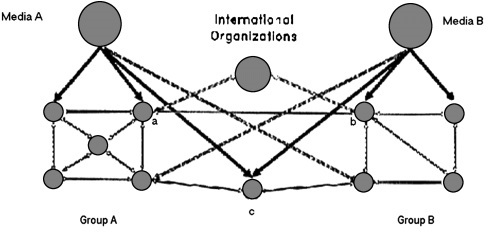
\includegraphics[width=10cm]{Figures/structuralmodel.jpg}
\caption{Structural Model of intercultural communication \citep{Barnett2005}}
\label{fig:figure1}
\end{figure}

In each of the three corpus analyses, we see examples of how global institutions and media shape the intercultural context. In the GM seed debate, a key theme is the dominance of global corporations and, in particular, the patent rights that have been granted through waves of international trade agreements and accompanying legislation. In the pipeline and mining debates, we consider the role of media in advancing stereotypes and contributing to in-group/out-group perceptions. In some cases, the presence of international institutions is used to label critics and environmentalists as outsiders who have little direct concern for the local community. 

To summarize, while conventional structural models suggest increased globalization will facilitate and ease intercultural encounters, contemporary reactions against globalization question this assumption. A multilevel discourse approach allows the researcher to carefully consider challenges globalization and mass media pose to effective intercultural communication.   

\subsection{The Role of Corpus-Based Methods}

A final methodological implication to consider is the role of corpus-based methods in intercultural research. Using secondary, corpus data runs counter to much ICC research given that many scholars in the field have limited intercultural communication to face-to-face interactions \cite[179]{Gudykunst2001}. However, in light of advances of globalization and information technology, we can consider that most intercultural interactions are now mediated by electronic devices, social media, and other technologies. Corpus methods allow for the systematic study of these interactions. Moreover, multimodal and audio-visual data permit the study of face-to-face interactions via corpus methods. However, it may be the case that corpus methods are not the entirety of an intercultural analysis. For instance, corpus data might be used to identify the context of intercultural communication, while the communicative interactions themselves are investigated through more direct methods and primary sources. 

The three corpora in this dissertation are a testament to the variety of topics and aspects of human communication that can be studied. Each corpus is quite distinct in terms of its contents as well as the dimensions of human communication contained within. The volume of data on the World Wide Web allows for the creation of specialized corpora. The data then provide a window into regions of language and communication that would otherwise be difficult to study had other data sources been used. That said, drawbacks of internet data must be kept in mind. When data is distributed via commercial search engine algorithms, issues of diversity, bias, and representativeness must be carefully considered. Given the plethora of search engine optimization and advertising copy, one must be aware of how the ``discourse of advertising'' \citep[99]{CurtisCollins2019} might overshadow authentic communication.

\section{Nature within ICC Research}

This dissertation has implications for how the natural world is approached in ICC research. While the previous chapter outlined conceptual principles along these lines, it remains unclear how these principles can be integrated into the main currents of intercultural communication research. This section will discuss the theme further, this time with more explicit reference to ICC literature.  

Part of the motivation for this dissertation is that ecology has not been a common theme in ICC research. This is not to say it has been entirely absent; rather, the topic is in need of a more firm grounding in the discipline. Where it has been factored into ICC research, nature has often been considered as a dimension of culture. In their \textit{Cultural Orientation Framework}, \cite{Kluckhohn1961} include ``orientation'' to the environment as one of six dimensions with which a society can be categorized. These authors identify subjugation, harmony, and mastery as culturally variable orientations to nature. Even if not assigned its own dimension, nature also falls under other categories. For instance, protection of the environment is considered under ``Universalism'' as a value priority with which Schwartz and colleagues compare countries \citep{Sagiv2000}. In the more recent \textit{Globe Study} \citep{House2004}, concern for the natural world could be considered part of the ``Future Orientation,'' one of the nine dimensions of cultural variability.

\subsection{Interpretive \& Critical Scholarship}

Previous studies have often approached orientation to nature as a statistical variable. The studies mentioned above, for example, use survey data as well as interviews to place different cultures on a relative scale. By contrast, the multilevel framework, together with conceptual principles proposed in the previous chapter, asks us to take a different methodological approach to nature than has been commonly observed in ICC research. Rather than viewing nature as among a handful of horizontal cultural variables, a multilevel approach hierarchically organizes the variables (as levels) from the macro to micro context. The ecological context is the macro level and is thus a starting point for understanding human communication. Nature and the environment form nothing less than semiotic context of human culture and communication. The environment is thus no longer one cultural variable among others, but analysis of human communication begins at the ecological level. The ecological level might focus on specific ecological themes and issues (as is the case in this dissertation), but could also include physical location, infrastructure, technology, soundscape, and other precursors to human communication.  

Based on the observations in this dissertation, we can conclude that the role of nature in communication and culture is too nuanced and complex to treat it as a quantitatively measured category. Qualitative, interpretive work is necessary before making generalizations about the meaning of nature for particular groups and cultures. Moreover, when collecting data through interviews and surveys, scholars need to be weary of \citeauthor{Beattie2016}'s (\citeyear{Beattie2016}) observation that there is a difference between what people explicitly say and how they feel about environmental issues. This observation is supported by the nonverbal study in Chapter 5, where we see how feelings and emotions associated with place and environment are often best understood through nonverbal, cognitive level analysis. Alongside primary sources (which may include interviews and surveys), multimodal corpus data of real communication events may be necessary to capture implicit feelings and attitudes.

With respect to critical approaches, this dissertation points to the importance of the analysis of political and economic dimensions of environmental issues and how these intersect with culture. Environmental and natural resource issues lie at the core of livelihoods and political/economic power. Alongside interpretive approaches, there is a need for the critical analysis of ecological-related communication. In each of the three analyses in this dissertation, the economic aspect was arguably the most contentious and gave rise to the strongest emotions. Critical approaches are needed to consider how culture is constructed in environmental discourse and how these constructions benefit certain interests.    

\subsection{Environmental Movements as Intercultural Spaces}

ICC scholarship is concerned with forums and spaces in which intercultural encounters take place. These forums and spaces are many and are evolving rapidly in global, technological society. At the same time, spaces for free, authentic communication are under threat. In line with critical analysis, we can consider that many communicative spaces are mediated and controlled by private interests. Social media, mobile networks, the built environment, etc., are most often owned and managed by corporate interests. One might question, therefore, where genuine intercultural encounters can take place.

In the previous chapter, the idea of the public sphere was introduced as precondition for deliberation. Specifically, it is proposed that the public sphere is a requirement for intercultural communication. Of particular interest for intercultural scholarship is how environmental protest movements are \textit{spaces of appearance} that reestablish the public sphere in societies where discursive spaces have been largely privatised. \cite*{Arendt1958a} describes space of appearance as ``the space where I appear to others as others appear to me, where men exist not merely like other living or inanimate things but make their appearance explicitly'' (198). The space of appearance is a precondition for the public sphere insofar as it ``precedes all formal constitution of the public realm and the various forms of government'' (199).

The notion of public sphere is particularly important in understanding communication related to the Dakota Access Pipeline. As discussed in Chapter 4, discourses in this corpus indicate a turning away form, and critique of, prevailing social institutions. The communication of pipeline opponents might be understood as an attempt to form alternative ``discursive spaces'' \citep[61]{Hauser1999a}. When peaceful pipeline demonstrators set up encampments in North Dakota, they were creating a discursive space. This can be understood as an establishment of the public sphere, after more official mechanisms (political, legal, media, etc.) were deemed futile. The socio-economic level of analysis in Chapter 4 discusses the closing off or denial of the public sphere. Quotes reveal how the pipeline protesters re-created the public sphere through a \textit{space of appearance}. 

Certain statements of protestors refer to a lack of voice and representation. The closing off of the public sphere, discussed in the socio-economic level of analysis, is expressed in the following statements:   

\begin{footnotesize}
\begin{itemize}
\item[] \texttt{We don't ever hear the narrative of indigenous people. We hear people writing our narratives for us.\newline 
\textit{-Eryn Wise, Council communications director}}
\newline
\item[] \texttt{It's just been escalating to that point where we have to use our phones to just show our side of our story. \newline 
\textit{-E'sha Hoferer, protester}}
\end{itemize}
\end{footnotesize} 

The denial of the public sphere experienced by protestors results in a sense of distance or alienation from social/institutional structures (i.e. civilization). As \cite*{Arendt1958a} states, ``alienation is the atrophy of the space of appearance'' (209). In other words, as alienation in a society grows, the space of appearance declines, and vice versa.

The protest site can be seen as the reestablishment of a place of appearance for those who felt it had been denied in the wider society. In Spring 2016, Standing Rock Sioux elder LaDonna Brave Bull Allard established a camp both as a centre of resistance to the pipeline and as a defense of sovereignty. By the summer, the camp had grown to thousands of people. Those at the camp referred to themselves as ``Water Protectors.'' In light of the negative connotations of ``protester'' (as discussed in the cognitive-level of analysis), the ``Water Protectors'' moniker can be seen as a way to re-frame how pipelines opponents are perceived and understood. 

To conclude, this dissertation calls for a reconsideration of the topic of the natural world within ICC research. Through both interpretive and critical approaches, the natural world can be given a central place in the discipline. At a more practical level, debates about infrastructure and natural resources are important intercultural spaces where expressions of identity take place in the public sphere. 

\section{Intercultural Competence}

In response to the three analyses in this dissertation, one might ask how these or similar misunderstandings could be overcome. In other words, are there principles or best practices that would enable mutual understanding in the context of environmental and resource issues? The premise of this question is that improved, more effective communication is possible on the part of various individuals and groups involved in these debates. In this section we consider this question by way of the concept \textit{intercultural competence}. In the discussion that follows, the concept of intercultural competence is seen as helpful but also in need of reconsideration. It is helpful in that there are principles of intercultural competence that are crucial in these contexts. However, we also argue that some principles and normative underpinnings of intercultural competence may need to be reconsidered in light of environmental issues. 

In short, we argue that many competence models, particularly those employed in stakeholder and public relations, have premises and underpinnings which do not transfer well to communication about ecological issues. There has been a recognition of the need for ICC research and models which are distinct to professional disciplines, notably medicine and education. In the same way, this section argues for ICC to be investigated more specifically in the domain of natural resources and ecology.       

\subsection{Cognitive Complexity \& Intercultural Competence}

Intercultural competence is a term to describe ``appropriate and effective communication and behavior in intercultural situations'' \cite[xi]{Deardorff2009}.  Competent communication has referred to an ability to identify and obtain goals, predict the behaviors and responses of the other communicator, choose effective communication strategies, and so on. It entails an understanding of acceptable behavior and meeting expectations and demands of situations \citep[209]{Wiseman2001}. A definition of intercultural competence that is consistent with the intergroup/intercultural concepts of this dissertation is that of \cite*{Spitzberg2009}: 

\begin{quote}
 the appropriate and effective management of interaction between people who, to some degree or another, represent different or divergent affective, cognitive, and behavioral orientations to the world. (7)   
\end{quote}


Various characteristics and behaviors of intercultural competence have been developed by ICC scholars as well as in related fields such as communication, psychology, foreign language, and management studies \cite[53-78]{Spencer-Oatey2009}. This includes research in applied linguistics and discourse studies which address problematic communication (ibid, 65). Research on intercultural competence has generally found that it results from a combination of personal capacities (e.g. flexibility, language skills, open-mindedness) and contextual factors (e.g. shared goals, perceptions) \citep{Arasaratnam}. 

\cite{Ruben1976} identifies several elements of intercultural competence in the context of overseas assignments: empathy, respect, role behavior flexibility, orientation to knowledge, interaction posture, interaction management, and tolerance for ambiguity. Similarly, \cite{Hammer1978} identify three key abilities: dealing with psychological stress, communicating effectively, and establishing interpersonal relationships. \cite{Martin1993} develops a three-level typology for assessing intercultural competence in a consistent and comparable manner. At the most global level is higher-order cognition and behaviors. The next level consists of mid-range behaviors such as interaction management and rule conformity. The third consists of micro behaviors such as body language and proxemics \citep[see][210-11 for an overview]{Wiseman2001}. 

From the definitions and previous research, we can begin to see how intercultural competence is highly relevant to environmental debates. In line with Spitzberg and Chagnon's definition which addressed ``different or divergent affective, cognitive, and behavioral orientations to the world,'' the types of interactions we examine in this dissertation exemplify different affective, cognitive, and behavioral orientations to the \textit{natural} world. Each corpus analysis shows that people have divergent feelings and attitudes about the environment (affective); they often conceptualize and understand the natural world in very different ways (cognitive); finally, different people behave differently within and toward the biophysical environment and other species (behavioral). We can also see how competency skills and factors would contribute to understanding and positive outcomes in these situations. For instance, flexibility and open-mindedness are important in the cognitive orientation, facilitating understanding of the different ways people perceive and relate to nature. Empathy would be important in relation to the affective aspects of these issues, such as concerns about impacts on livelihoods or health. The contextual factors in competency models are also crucial in reaching positive outcomes. For instance, without identifying some shared goals between proponents and opponents, communication around natural resource projects will be doomed to fail.      

In light of the analyses in this dissertation, one aspect of intercultural competency that stands out is cognitive complexity. Cognitive complexity (or flexibility) is the ability to form versatile and nuanced perceptual categories and constructs \citep{Bieri1955}. \cite*{Pervin1984} defines this ability as 

\begin{quote}
an aspect of a person's cognitive functioning which at one end is defined by the use of many constructs with many relationships to one another (complexity) and at the other end by the use of few constructs with limited relationships to one another (simplicity). (507)
\end{quote} 

In intercultural competence, cognitive complexity has been identified as important in avoiding stereotypes and being perceptive to subtle racism \citep{Read2016}. \cite*{Gudykunst1995} also identifies cognitive complexity as crucial to managing uncertainty and anxiety in intercultural communication. While these aspects certainly apply to the observations in the present dissertation, there are other dimensions of cognitive complexity which could be emphasized when it comes to ecological issues. While intercultural communication has emphasized cognitive complexity as perceptual and communicative skills (e.g. perceiving nuanced differences), the analyses in this dissertation also points to the need for complexity in terms of abstract mental structures and frames. 

In the previous chapter we introduced the notion of surveyability and how surveyability bias is a barrier to understanding and communication. We propose that many misunderstandings we find in the corpus analyses are the result of different language games being played. For instance, if someone operating within a positivist/scientific language game is confronted with a statement expressing cultural identity, they will need to recognize that the entire framework of meaning has changed. In addition to this recognition, a new set of cognitive structures is necessary to communicate effectively within the `new' language game. As in the discourse on GM seed, these structures are often embodied and deeply embedded in a form of life.      

Cognitive complexity, then, might be described as an ability to navigate language games. It is an ability to avoid surveyability bias; that is, continuously questioning the assumption that one has the whole picture and context. This notion of complexity is consistent with that in existing intercultural competency literature, in that understanding others requires changing one's frame of reference \citep{Friedman2014}. This view of complexity diverges somewhat from prevailing models in that it places emphasis on abstract mental processes prior to perception and communication skills. This view of complexity also proposes a distinction between language facility and communicative skills versus the ability to recognize and `play' different language games.     

\subsection{Critiques of Intercultural Competence Theories}

Above we discussed cognitive complexity as an aspect of ICC competence that is transferable to ecological debates, albeit perhaps with a new emphasis. Here we consider more fundamental issues if ICC principles are applied to ecological debates of the type analyzed in this dissertation. There are two main issues discussed below. First, is the possibility that cultural blindness (avoiding the cultural context or frames) is a deliberate discourse strategy. Second, we propose that ICC competence has inherited some problematic premises from the rhetorical tradition in communication theory. These issues are briefly presented as a segue into the next section, ``Revisiting Intercultural Competence,'' which is a positive formulation of what might constitute ICC competence when it comes to ecological debates.   

\textbf{Intercultural Incompetence as a Deliberate Discourse Strategy}

Of course, the opposite of intercultural competence is intercultural \textit{in}competence. This incompetence might more aptly be described as a set of communicative and behavioural shortcomings. From a critical standpoint, one issue we encounter is the source or motivation of these shortcomings. Failures of intercultural communication have often been described as inadvertent oversights, due to some lack of awareness or communicative ability. However, there may also be cases where intercultural blindness is deliberate and strategic. In each of the analyses in the dissertation, we conclude that a principle source of misunderstanding is a tendency to shift away from the cultural context and frame the issues in more definitive and measurable terms. In all the analyses, one could postulate that this shift is strategic and beneficial to certain actors. Decontextualizing might be seen as a way of managing the discourse. Keeping the subject bound within the expertise of given groups (e.g. institutions, professional communities, corporations) helps ensure the legitimacy and authority of those groups is maintained.

The types of debates we examine in this dissertation are very high stakes economically. GM seed, pipelines, and mining projects all involve many billions of dollars. It can, therefore, be assumed that great care is taken with regard to how these topics are presented and discussed in the media and in public forums. To embed the discourse in entire histories and belief systems would be to acknowledge dimensions of the issues that might be problematic for proponents. For instance, if agrochemical corporations were to fully engage with the issues raised by peasant farmers in the Global South they would likely be undermining their own messaging. Similarly, if a mining or pipeline company were to discuss the time scale of a project in terms of multiple generations, the authority and certainty of their scientific claims would be undermined. The fundamental point is that notions of intercultural communication competency that stress individual capacities (e.g, language ability, openness) are not sufficient if avoiding the cultural context is a deliberate discourse strategy. 

\textbf{Intercultural Competency \& the Rhetorical Tradition}

A discussion of the strategic management of communication leads us to another aspect of ICC competence; namely, the theories and criteria used to determine what competent communication is. Based on \citeauthor{Craig1999a}'s (\citeyear{Craig1999a}) seven traditions in communication theory, we propose that common ICC competence theories are most closely aligned with the rhetorical tradition. Though perhaps implicitly, much competency research is based on notions of communication as a skill to achieve an end. In other words, communication is artful persuasion for the purpose of achieving one's goals. 

A rhetorical focus is understandable given the origins of the research. Traditionally intercultural communication research has been motivated by diplomacy, trade, going abroad, and intercultural business management \citep{Jensen2014}. Effective communication has been inseparable from the success of the institution, mission, or enterprise. Accordingly, effective communication is associated with the ability to achieve desired outcomes. Competent communication is described as the ability ``to control and manipulate'' one's social environment to obtain goals \cite[209]{Wiseman2001}. This emphasis is also not a surprise given that the rhetorical tradition is deeply embedded in Western scholarship. As \cite*{Littlejohn1996} points out, rhetoric is the ``primary source of ideas about communication...dating back to ancient times'' (117). 

Granted, the wide variety of intercultural competency theories do not all conform to an instrumental view of communication. Yet, much of the research does operate under the assumption that with enough knowledge, it is possible to predict how to behave in intercultural settings \citep{Jensen2014}. The implicit assumption is that communication is a skill and art.

With respect to ecological communication, we propose that intercultural competency take a sharper turn away from the rhetorical tradition. The critiques of this tradition are not new, but brought into focus in ecological discourses. The following are three perspectives adapted from \citeauthor{Craig1999a} (\citeyear[134]{Craig1999a}), that are particularly relevant in light of the analyses in this dissertation.

\begin{itemize}

    \item \textit{Phenomenological perspective}: strategic communication is inauthentic and often counterproductive. In debates analyzed in previous chapters, we saw that trust is a major issue. People are able to `see through' impression management and this type of communication does more harm than good.
    
    \item \textit{Critical perspective}: rhetoric reflects instrumentalist and individualist ideologies. The rhetorical management of communication is an instrument of power. Moreover, we can consider that communication competency is often a skill that an individual has. In environmental debates, there is a need for notions of competent communication in terms of collective cognition of communities and groups.  
    
    \item \textit{Cybernetic perspective}: complex systems involve technical problems rhetoric fails to grasp. Ecological systems are complex and technical. It is simplistic and even dangerous to view communication about these systems as strategic and persuasive.

\end{itemize}

Based on three perspectives from traditions in communication theory (cybernetic, phenomenological, and critical) we can develop notions of competency that counter the rhetorical emphasis which is commonplace today. Below these perspectives are outlined in order to sketch out a notion of intercultural competence that is compatible with ecological discourse.

\subsection{Revisiting Intercultural Competence}

In response to the above critiques, one could ask what effective communication looks like in the context of environmental debates. The short answer is that, at least when it comes to multilevel issues of the type we see in this dissertation, there is not a simple list of traits or principles. At the same time, effective communication in environmental debates will not be a complete departure from existing research on intercultural competence. While strategic and instrumental modes of communication are to be avoided, there are other aspects of competency that remain essential.

\textbf{Phenomenology, Mindfulness and Cognitive Complexity}

One such aspect, introduced above, is cognitive complexity. One might ask for a more specific characterization of cognitive complexity with some details as to how it can be measured or developed. It can be stressed that the cognitive complexity we are referring to is not a matter of obtaining more systematic knowledge or technical skills. It would seem, rather, to entail a capacity to transcend one's own assumptions, frames, and categorization schema. We might consider how authentic communication, as understood in the phenomenological tradition, is reflective of this capacity. In this tradition, understanding begins with prereflective experience, embodied in a shared lifeworld \cite[138]{Craig1999a}. 

To help operationalize the phenomenological tradition, we can relate it to the notion of mindfulness. Though mindfulness is a relatively recent topic in communication theory, it can be situated within a long-standing discussion of phenomenology or the conscious processing of phenomena \citep{Brown2009}. \citeauthor{Ting-Toomey2015} (\citeyear{Ting-Toomey2015}) makes an explicit connection between mindfulness and intercultural competence. Mindfulness involves an in-the-moment, holistic presence in order to ``tune in to our own cultural and personal habitual assumptions in scanning a communication scene'' (620). \citeauthor{Ting-Toomey2015} describes mindfulness as being present within a ``multilayered cultural system'' with deep understanding of ``micro and macro layers'' of culture (621-24). Here, we can see parallels with the multilevel framework employed in this dissertation. Cognitive complexity involves perception of the nuanced lifeworld together with a holistic overview of how multilayered dimensions hang together. 

Specifics of how to build and implement this type of cognition are beyond the current scope and perhaps a direction for additional research. One avenue for research is the development of cognitive complexity, which might entail humanities education, interdisciplinary thinking, and learning that facilitates embodied awareness.         

\textbf{Critical Theory and the Communicative Context}

Previously we discussed a number of possible aspects of ICC competence that are best addressed by a critical theoretical approach. Specifically, these aspects relate to strategic and managed communication, often with the goal of material gain or power. One could argue that the mindfulness/phenomenological approach described above is somewhat naive when faced with realities of injustice, oppression, or manipulation. Accordingly, we propose that there is an crucial element of ICC competence that involves unmasking discourse and taking part in reflective social action.

Unmasking involves awareness and opposition to conditions that inhibit authentic dialogue. From a critical standpoint, mindful and authentic communication are worthy ends but often not achievable in reality: ``phenomenological dialogue represents an ideal form of communication, but one that existing sociocultural conditions may render unlikely'' \cite[148]{Craig1999a}. In the previous chapter, we discuss the public sphere as a precondition for intercultural communication and how, in the contemporary neoliberal order, the public sphere is encroached upon by private interests. ICC competence might involve a critical/contextual awareness of how power and material interest play into communication. To take this a step further, competence could involve a fostering of alternative communicative spaces.      

More than other traits discussed thus far, this critical notion of ICC competence departs from conventional competency research. In contrast to communication competency focused on operating successfully in the social world, a critical perspective seeks change and action. The critical approach further compels us to question the aims and assumptions behind competency, particularly given that intercultural competence research has been most strongly influenced by research from economically developed parts of the world \citep{Arasaratnam}. The goal of maintaining a positive social impression is overshadowed by the possibility that people in less powerful positions may be disadvantaged in terms of maintaining a positive impression \citep{Spencer-Oatey2009}.

With these critical considerations, characteristics important to ICC competence might include: awareness of power and privilege, willingness to challenge convention, and the ability to foster spaces for authentic dialogue in the public sphere. 

\textbf{Cybernetics and the Ecological System}

The final consideration for ICC competence in ecological debates is the technical and scientific nature of the subject. Effective communication will need to convey how human and natural systems interact. Communication in the cybernetic tradition ``explains how all kinds of complex systems, whether living or nonliving...are able to function, and why they often malfunction'' \cite[141]{Craig1999a}. Without requiring expert knowledge of the biological and ecological sciences, cybernetics draws analogies between human communication, artificial and natural systems. The cybernetic tradition may help us formulate an idea of effective communication in the Anthropocene. Though an area in need for further study, interactions between the physical environment and consciousness in terms of both information transfer and semiotics could expand the scope of ICC research.     


\section{Conclusion}

The primary aim of this dissertation was to develop conceptual principles that could form the basis of future work. It goes without saying, therefore, that the directions for further research are wide open. Before venturing into new directions it is necessary to acknowledge some of the limitations of this present dissertation, which might compel one to revisit the premises and methods that were employed to arrive at the conclusions. 

\subsection{Limitations}

Two of the most apparent limitations are (i) the reliance on secondary sources and lack of field work; and (ii) the composition of the corpora. 

\begin{itemize}

    \item \textit{Secondary sources}: One limitation, already discussed in Chapter 2, is that this dissertation did not involve field work. The reliance on secondary sources was deliberate and consistent with the aims of the corpus analysis. However, these methods precluded depth in ethnographic analysis. Accordingly, further research might combine the methods employed in this dissertation with interviews or field research where questions are pursued in more depth and validated through follow up interviews. 
    
    \item \textit{Composition of corpora}: There are also a number of limitations related to the corpora. As highlighted in a previous section, the corpora were confined to the English language and their status as intercultural corpora could be questioned. The corpora were constructed according to ecological themes, rather than cultural/linguistic factors. For intercultural research, explicitly assembling a corpora consisting of language from different cultural backgrounds could be advantageous. Also, given that data was taken from media sources, communication was not part of the flow of everyday interactions. Further corpus research might aim at gathering more data in the form of dialogue and raw linguistic data. 
    
    \item \textit{Theoretical focus}: The stated aim was to develop a conceptual framework. However, the communication problems are very real and the ecological issues urgent. One could see the focus on concepts and theory as a limitation of this dissertation. There are no prescriptive solutions proposed. That said, there is no reason why the approach used here could not be applied by practitioners involved in current and future environmental debates. 
    
\end{itemize}

\subsection{Directions for Further Research}

The underlying message of this dissertation is that the relationship between human culture, communication, and the natural world is full of complexity and richness. The relation between identity and the environment is one that emerged throughout the dissertation and could be explored in much more depth. More specifically, the connection with self esteem could be pursued.

As mentioned in the opening of this section, previous intercultural communication studies have treated the environment as a variable in cross-cultural comparisons. This dissertation makes the case that nature take more central, crucial place in culture and identity. Throughout the corpora, we found examples of how the natural world is closely bound with cultural identity. Moreover, this fusion of culture and nature seems to be a source of confidence and self esteem. In modern, pluralistic societies, cultural identity is often beneath the surface and something that we do not explicitly state. In environmental debates, cultural identity does seem to come to the surface, however. Why this is the case remains uncertain, but the link to self esteem might be considered. \cite{camilleri1990stratégies} outline ways in which migrants manage their identities in everyday interactions (at times minimizing it, or highlighting it) to preserve or enhance self esteem \citep{Frame2014}. The proceeding corpus analyses suggest that in natural resource debates cultural identity is often highlighted as a source of self esteem.

Another avenue for further research is the relation between cultural constructions and political/economic power. This might take the form of an historical, postcolonial analysis of how cultural groups were (and continue to be) marginalized due to the pursuit of land and extraction of natural resources. Given the depth and complexity of this theme, a more specific thread might be pursued such as, for instance, historical corpus analyses of natural resource discourses. Along the same lines, a theme for further consideration is the material/economic drivers of cultural discourses. Earlier in the chapter it was proposed that culture might be deliberately avoided as a discourse strategy. Further research might ask if there is a material interest in not addressing the cultural context. Or, similarly, one might ask if there are interests in reducing culture to customs, artifacts, and behaviours that are more or less divorced from the often difficult issues related to economic and political power. 

Finally, an implication for further research is the need for intercultural scholarship that combines the critical and humanistic traditions. Intercultural scholarship demands modes of thinking that are fostered through the humanities and the arts: grappling with nuances, thinking critically, awareness of one's own epistemological position, and remaining open to diverse perspectives \citep{Nussbaum1997a,Nussbaum2010a}. At the same time, scholarship can identify social and economic structures that oppress not only human cultures, but the natural world. 
  % Results and Discussion

%% ----------------------------------------------------------------
% Now begin the Appendices, including them as separate files

\addtocontents{toc}{\vspace{2em}} % Add a gap in the Contents, for aesthetics

\appendix % Cue to tell LaTeX that the following 'chapters' are Appendices

\chapter{Appendix 1}
\lhead{\textit{Appendix 1}}
This appendix contains the data analysis (using Python) for the analysis described in Chapter 3. The data is a corpus consisting of articles and webpages representing different perspectives on Genetically Modified (GM) Seed. The data was collected manually using a search engine. Resulting webpages were then determined as representing either anti-GM or pro-GM seed perspectives. The text was then cleaned and saved in 2 separate files: \textit{anti-gmo.txt} and \textit{pro-gmo.txt}.



Raw data is available in the folder \textit{Analysis 1} in a in a GitHub repo: \href{https://github.com/craigmateo/multilevel_corpus}{https://github.com/craigmateo/multilevel\_corpus}

The sections below contain a description of each analysis carried out as well as the corresponding Python code and the output from running that code. 

\section{Pre-processing}

The code below reads the 2 \textit{txt} files and does preprocessing on the text. The preprocessing consists of:

1. \textbf{Noise removal} (removal of punctuation, special characters, digits)
2. \textbf{Normalization} (stemming, lemmatization, removal of stopwords) 

Exceprts from the each preprocessed subcorpus are then printed.

\textbf{Code: Pre-processing}

\begin{lstlisting}
# Open the anti_gmo.txt supcorpus
anti_file = open("anti_gmo.txt", "r", encoding="UTF-8")
anti_lines = anti_file.readlines()
# Open the anti_gmo.txt supcorpus
pro_file = open("pro_gmo.txt", "r", encoding="UTF-8")
pro_lines = pro_file.readlines()
anti_lines = [line[:-1] for line in anti_lines]
pro_lines = [line[:-1] for line in pro_lines] 
# Libraries for text preprocessing
import re
import nltk
#nltk.download('stopwords')
from nltk.corpus import stopwords
from nltk.stem.porter import PorterStemmer
from nltk.tokenize import RegexpTokenizer
#nltk.download('wordnet') 
from nltk.stem.wordnet import WordNetLemmatizer
##Creating a list of stop words
stop_words = set(stopwords.words("english"))
corpus_antiPRE = []
corpus_anti = []
for i in range(0, len(anti_lines)):
    #Remove punctuation
    text = re.sub('[^a-zA-Z]', ' ', anti_lines[i])
    #Convert to lowercase
    text = text.lower()
    #remove tags
    text=re.sub("&lt;/?.*?&gt;"," &lt;&gt; ",text)
    # remove special characters and digits
    text=re.sub("(\\d|\\W)+"," ",text)
    corpus_antiPRE.append(text)
    ##Convert to list from string
    text = text.split()
    ##Stemming
    ps=PorterStemmer()
    #Lemmatisation
    lem = WordNetLemmatizer()
    text = [lem.lemmatize(word) for word in text if not word in  
            stop_words] 
    text = " ".join(text)
    corpus_anti.append(text)
corpus_proPRE = []
corpus_pro = []
for i in range(0, len(pro_lines)):
    #Remove punctuation
    text = re.sub('[^a-zA-Z]', ' ', pro_lines[i])
    #Convert to lowercase
    text = text.lower()
    #remove tags
    text=re.sub("&lt;/?.*?&gt;"," &lt;&gt; ",text)
    # remove special characters and digits
    text=re.sub("(\\d|\\W)+"," ",text)
    corpus_proPRE.append(text)
    ##Convert to list from string
    text = text.split()
    ##Stemming
    ps=PorterStemmer()
    #Lemmatisation
    lem = WordNetLemmatizer()
    text = [lem.lemmatize(word) for word in text if not word in  
            stop_words] 
    text = " ".join(text)
    corpus_pro.append(text)
anti_text = " ".join(corpus_anti)
pro_text = " ".join(corpus_pro)
print("Anti-GM Seed Excerpt:" + "\n" + "-"*30 + "\n" + anti_text[1000:1100])
print("\n")
print("Pro-GM Seed Excerpt:" + "\n" + "-"*30 + "\n" + pro_text[1000:1100])
\end{lstlisting}

\textbf{Output: Text excerpts}
\begin{footnotesize}
Anti-GM Excerpt:\newline
--------------------\newline
e small scale farmer form cooperative wanted support department make attractive offer provide farmin

Pro-GM Excerpt:\newline
--------------------\newline
ogy frequently asked question gmos blame mass suicide indian farmer find suicide rate male indian fa
\end{footnotesize}

\section{Word Counts}
Separate word counts are taken for each subcorpus. One count is taken with only noise removal and another with both noise removal and normalization. 

\textbf{Code: Word counts}

\begin{lstlisting}
anti_textPre = " ".join(corpus_antiPRE)
pro_textPre = " ".join(corpus_proPRE)
num_words_antiPRE = format(len(anti_textPre.split()),",")
num_words_proPRE = format(len(pro_textPre.split()),",")
num_words_anti = format(len(anti_text.split()),",")
num_words_pro = format(len(pro_text.split()),",")
print("\n" + 'Noise Removal:' + "\n" + "-"*30)  
print("anti_gmo.txt: " + str(num_words_antiPRE))
print("pro_gmo.txt: " + str(num_words_proPRE))
print("\n" + 'Noise Removal & Normalization:' + "\n" + "-"*30)  
print("anti_gmo.txt: " + str(num_words_anti))
print("pro_gmo.txt: " + str(num_words_pro))
\end{lstlisting}

\textbf{Output: Word counts for each subcorpus}
\begin{footnotesize}
Noise Removal:\newline
--------------------\newline
anti-gmo.txt: 224,883\newline
pro-gmo.txt: 162,850

Noise Removal \& Normalization:\newline
--------------------\newline
anti-gmo.txt: 134,844\newline
pro-gmo.txt: 101,238
\end{footnotesize}

\section{Url Domain Analysis}

The files urls-anti-gmo.txt and urls-pro-gmo.txt list the urls used to collect the data. The two cells below parse the urls to determine distribution of top-level domains (tlds) and then plot the results in a pie chart. A random sample of 3 urls is also printed.

The plot clearly shows that the anti-gmo.txt consists of more .org domains and the pro-gmo.txt consists of more .com domains. This is might suggest that the anti-gmo data is more likely to come from NGOs or non-corporate institutions.

\textbf{Code: tlds (anti-GM)}

\begin{lstlisting}
# Open the anti
anti_urls = open("...\urls_anti_gmo.txt", "r", encoding="UTF-8")
anti_urls_lines = anti_urls.readlines()
tld_file = open("..\tlds.txt", "r", encoding="UTF-8")
tlds = tld_file.readlines()
import re
import matplotlib.pyplot as plt
tld_counts_anti = []
for url in anti_urls_lines:
    ind = [m.start() for m in re.finditer('/', url)][2]
    if url[ind-4] == ".":
        tld_counts_anti.append(url[ind-3:ind])
    if url[ind-3] == ".":
        tld_counts_anti.append(url[ind-2:ind])
from collections import Counter
counts_anti = Counter(tld_counts_anti)
print("total urls: " + str(len(anti_urls_lines))+"\n" )
print("Random sample of anti_gm urls:")
from random import sample
chosen_anti = sample(anti_urls_lines, 3)
for url in chosen_anti:
    print(url[0:-1])
print(counts_anti.most_common())
plot1 = plt.pie([float(v) for v in counts_anti.values()],... 
labels=[k for k in counts_anti], labeldistance=1.05, radius=1.8)
\end{lstlisting}

\textbf{Output: tlds (anti-GM)}


\begin{footnotesize}
total urls: 89

Random sample of anti-gm urls:

https://www.fondazioneslowfood.com/en/protecing-food-biodiversity-in-colombia/\newline
https://www.independentsciencenews.org/health/millions-spent-who-is-to-blame-failure-gmo-golden-rice/\newline
http://www.ipsnews.net/2008/07/agriculture-south-africa-small-farmers-pushed-to-plant-gm-seed


Top Level Domains (Anti-GM)\newline
----------------------------\newline
[('org', 39), ('com', 29), ('net', 5), ('edu', 4), ('ca', 3), ('uk', 2), ('nl', 2), ('br', 1), ('eu', 1), ('io', 1), ('za', 1)]
\end{footnotesize}

\begin{figure}[H]
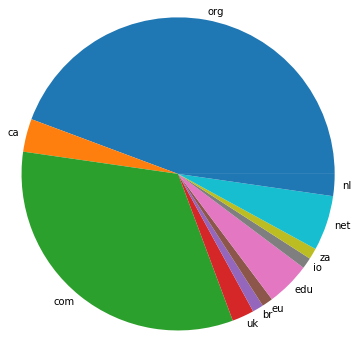
\includegraphics[width=7cm]{Figures/urls_1.png}
\end{figure}

\textbf{Code: tlds (pro-GM)}

\begin{lstlisting}
pro_urls = open("...\urls_pro_gmo.txt", "r", encoding="UTF-8")
pro_urls_lines = pro_urls.readlines()
tld_counts_pro = []
for url in pro_urls_lines:
    ind = [m.start() for m in re.finditer('/', url)][2]
    if url[ind-4] == ".":
        tld_counts_pro.append(url[ind-3:ind])
    if url[ind-3] == ".":
        tld_counts_pro.append(url[ind-2:ind])
print("total urls: " + str(len(pro_urls_lines))+"\n" )
print("Random sample of pro_gm urls:")
from random import sample
chosen_pro = sample(pro_urls_lines, 3)
for url in chosen_pro:
    print(url[0:-1])
counts_pro = Counter(tld_counts_pro)
print(counts_pro.most_common())
import matplotlib.pyplot as pyplot
plot2 = plt.pie([float(v) for v in counts_pro.values()],... 
labels=[k for k in counts_pro], labeldistance=1.05, radius=1.8)
\end{lstlisting}

\textbf{Output: tlds (pro-GM)}
\begin{footnotesize}
total urls: 91

Random sample of pro-gm urls:

https://bizfluent.com/info-8082116-positives-gmo.html\newline
https://www.marketplace.org/2016/08/09/world/sugar-beet-farmers-mull-objections-gmos\newline
https://www.bayer.com/en/position-on-genetic-engineering-straightforward.aspx
\end{footnotesize}

Top Level Domains (Pro-GM)\newline
----------------------------\newline
[('com', 50), ('org', 25), ('edu', 5), ('ca', 3), ('uk', 2), ('gov', 1), ('net', 1), ('cl', 1), ('in', 1), ('au', 1), ('ie', 1)]

\begin{figure}[H]
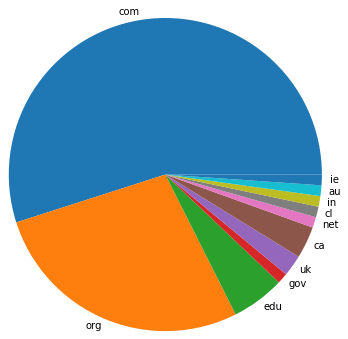
\includegraphics[width=7cm]{Figures/urls_2.png}
\end{figure}

\section{Keywords and top N-grams}

Top n-grams (sequences of \textit{n} words) were determined by taking the top frequencies on an absolute basis (i.e., not using a reference corpus for comparison). After removing stop words, the 20 most frequent uni-grams, bi-grams, and tri-grams (1-, 2-, and 3-word sequences) are determined for each corpus.

Code in this section is adapted from:\newline 
\small{https://medium.com/analytics-vidhya/
automated-keyword-extraction-from-articles-using-nlp-bfd864f41b34}

\textbf{Code: Keywords (anti-GM)}

\begin{lstlisting}

from sklearn.feature_extraction.text import CountVectorizer
import re
cv=CountVectorizer(max_df=0.8,stop_words=stop_words,
max_features=10000, ngram_range=(1,3))
X=cv.fit_transform(corpus_anti)
list(cv.vocabulary_.keys())[:10]
import pandas
#Most frequently occuring words
def get_top_n_words(corpus, n=None):
    vec = CountVectorizer().fit(corpus)
    bag_of_words = vec.transform(corpus)
    sum_words = bag_of_words.sum(axis=0) 
    words_freq = [(word, sum_words[0, idx]) for word, idx in      
                   vec.vocabulary_.items()]
    words_freq =sorted(words_freq, key = lambda x: x[1], 
                       reverse=True)
    return words_freq[:n]
#Convert most freq words to dataframe for plotting bar plot
top_words = get_top_n_words(corpus_anti, n=20)
top_df = pandas.DataFrame(top_words)
top_df.columns=["Word", "Freq"]
print(top_df)
#Barplot of most freq words
import seaborn as sns
sns.set(rc={'figure.figsize':(13,8)})
g = sns.barplot(x="Word", y="Freq", data=top_df)
g.set_xticklabels(g.get_xticklabels(), rotation=30)
\end{lstlisting}

\textbf{Output: Keywords (anti-GM)}

\begin{table}[H]
\begin{footnotesize}
\begin{tabular}{lll}
0  & seed        & 1749 \\
1  & food        & 1678 \\
2  & crop        & 1316 \\
3  & gm          & 1205 \\
4  & indigenous  & 1142 \\
5  & farmer      & 1107 \\
6  & people      & 1001 \\
7  & monsanto    & 656  \\
8  & right       & 630  \\
9  & traditional & 608  \\
10 & plant       & 540  \\
11 & use         & 510  \\
12 & also        & 499  \\
13 & land        & 483  \\
14 & genetically & 468  \\
15 & maize       & 465  \\
16 & cultural    & 454  \\
17 & company     & 424  \\
18 & community   & 416  \\
19 & corn        & 416 
\end{tabular}
\end{footnotesize}
\end{table}

\begin{figure}[H]
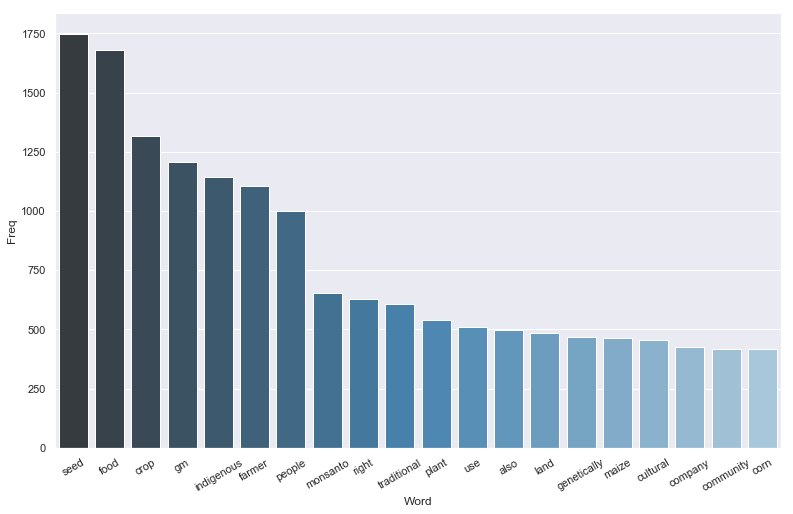
\includegraphics[width=14cm]{Figures/bar1.png}
\end{figure}

\textbf{Code: Keywords (pro-GM)}

\begin{lstlisting}
X=cv.fit_transform(corpus_pro)
list(cv.vocabulary_.keys())[:10]
#Convert most freq words to dataframe for plotting bar plot
top_wordsPRO = get_top_n_words(corpus_pro, n=20)
top_dfPRO = pandas.DataFrame(top_wordsPRO)
top_dfPRO.columns=["Word", "Freq"]
print(top_dfPRO)
#Barplot of most freq words
sns.set(rc={'figure.figsize':(13,8)})
g1 = sns.barplot(x="Word", y="Freq", data=top_dfPRO,  palette="Blues_d")
g1.set_xticklabels(g1.get_xticklabels(), rotation=30)
\end{lstlisting}

\textbf{Output: Keywords (pro-GM)}

\begin{table}[H]
\begin{footnotesize}
\begin{tabular}{lll}
0  & crop       & 1979 \\
1  & gm         & 1977 \\
2  & ha         & 1120 \\
3  & impact     & 991  \\
4  & technology & 712  \\
5  & million    & 708  \\
6  & use        & 688  \\
7  & food       & 685  \\
8  & ht         & 666  \\
9  & farmer     & 639  \\
10 & soybean    & 627  \\
11 & herbicide  & 618  \\
12 & year       & 617  \\
13 & cotton     & 566  \\
14 & cost       & 507  \\
15 & farm       & 498  \\
16 & carbon     & 498  \\
17 & yield      & 486  \\
18 & seed       & 469  \\
19 & country    & 456 
\end{tabular}
\end{footnotesize}
\end{table}

\begin{figure}[H]
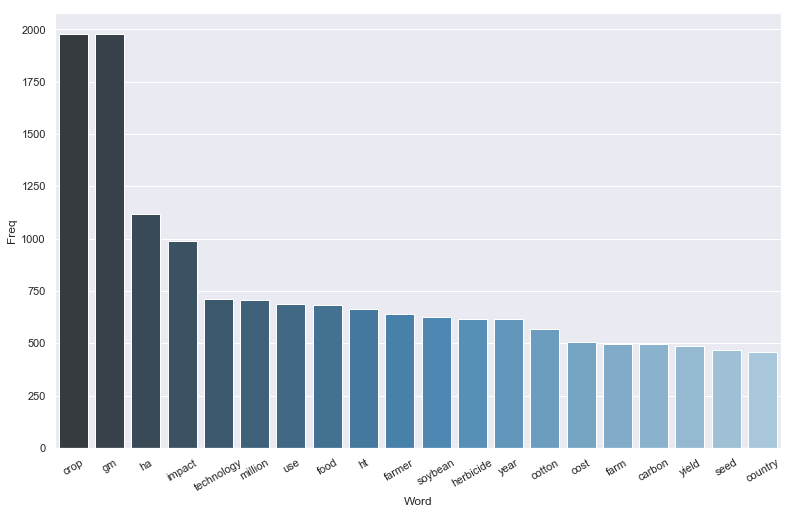
\includegraphics[width=14cm]{Figures/bar2.png}
\end{figure}

\textbf{Code: Bi-grams (anti-GM)}

\begin{lstlisting}
#Most frequently occurring Bi-grams
def get_top_n2_words(corpus, n=None):
    vec1 = CountVectorizer(ngram_range=(2,2),  
            max_features=2000).fit(corpus)
    bag_of_words = vec1.transform(corpus)
    sum_words = bag_of_words.sum(axis=0) 
    words_freq = [(word, sum_words[0, idx]) for word, idx in     
                  vec1.vocabulary_.items()]
    words_freq =sorted(words_freq, key = lambda x: x[1], 
                reverse=True)
    return words_freq[:n]
top2_words = get_top_n2_words(corpus_anti, n=20)
top2_df = pandas.DataFrame(top2_words)
top2_df.columns=["Bi-gram", "Freq"]
print(top2_df)
#Barplot of most freq Bi-grams
import seaborn as sns
sns.set(rc={'figure.figsize':(13,8)})
h=sns.barplot(x="Bi-gram", y="Freq", data=top2_df, palette="Blues_d")
h.set_xticklabels(h.get_xticklabels(), rotation=45)
\end{lstlisting}

\textbf{Output: Bi-grams (anti-GM)}

\begin{table}[H]
\begin{footnotesize}
\begin{tabular}{lll}
0  & indigenous people      & 576 \\
1  & gm crop                & 389 \\
2  & genetically modified   & 298 \\
3  & food sovereignty       & 164 \\
4  & per cent               & 159 \\
5  & non gm                 & 147 \\
6  & traditional food       & 141 \\
7  & genetically engineered & 129 \\
8  & indicator area         & 114 \\
9  & http www               & 112 \\
10 & food security          & 111 \\
11 & biocultural diversity  & 104 \\
12 & united state           & 92  \\
13 & right food             & 80  \\
14 & food system            & 79  \\
15 & traditional knowledge  & 77  \\
16 & indigenous community   & 72  \\
17 & et al                  & 72  \\
18 & non gmo                & 70  \\
19 & food production        & 67 
\end{tabular}
\end{footnotesize}
\end{table}

\begin{figure}[H]
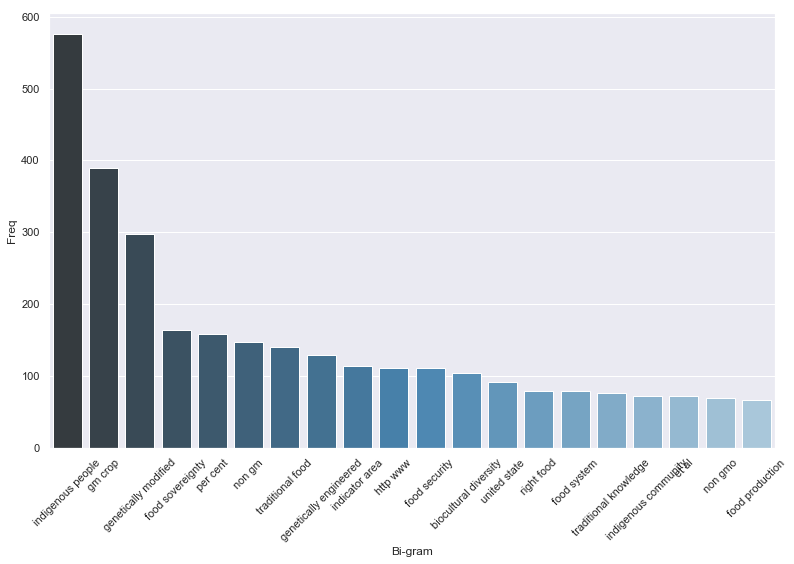
\includegraphics[width=14cm]{Figures/bar3.png}
\end{figure}

\textbf{Code: Bi-grams (pro-GM)}

\begin{lstlisting}
#Most frequently occurring Bi-grams
top2_wordsPRO = get_top_n2_words(corpus_pro, n=20)
top2_dfPRO = pandas.DataFrame(top2_wordsPRO)
top2_dfPRO.columns=["Bi-gram", "Freq"]
print(top2_dfPRO)
#Barplot of most freq Bi-grams
import seaborn as sns
sns.set(rc={'figure.figsize':(13,8)})
h=sns.barplot(x="Bi-gram", y="Freq", data=top2_dfPRO, palette="Blues_d")
h.set_xticklabels(h.get_xticklabels(), rotation=45)
\end{lstlisting}

\textbf{Output: Bi-grams (pro-GM)}

\begin{table}[H]
\begin{footnotesize}
\begin{tabular}{lll}
0  & gm ht                  & 569 \\
1  & gm crop                & 512 \\
2  & gm ir                  & 277 \\
3  & et al                  & 252 \\
4  & farm income            & 241 \\
5  & pg economics           & 209 \\
6  & crop impact            & 200 \\
7  & economics ltd          & 199 \\
8  & genetically modified   & 182 \\
9  & field eiq              & 175 \\
10 & ha ha                  & 162 \\
11 & ht soybean             & 158 \\
12 & biotech crop           & 138 \\
13 & million kg             & 136 \\
14 & environmental impact   & 134 \\
15 & active ingredient      & 129 \\
16 & cost saving            & 124 \\
17 & national academy       & 122 \\
18 & genetically engineered & 121 \\
19 & eiq ha                 & 120
\end{tabular}
\end{footnotesize}
\end{table}

\begin{figure}[H]
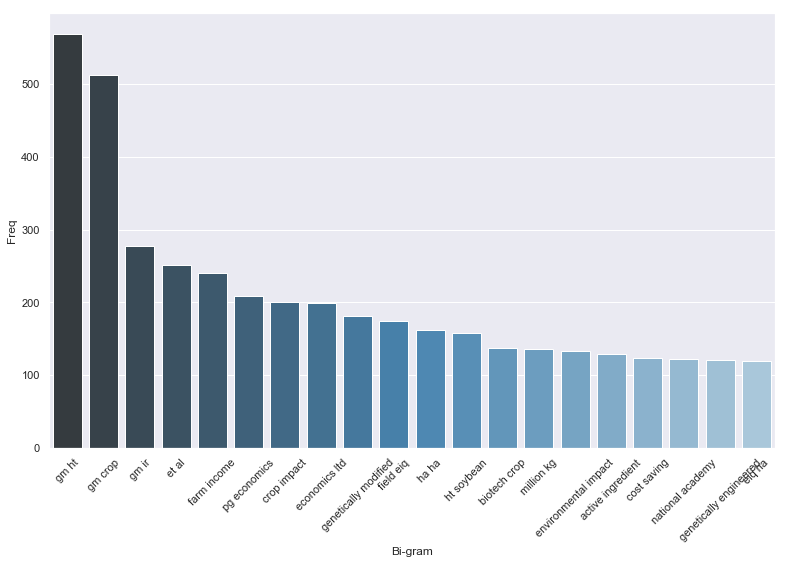
\includegraphics[width=14cm]{Figures/bar4.png}
\end{figure}

\textbf{Code: Tri-grams (anti-GM)}

\begin{lstlisting}
#Most frequently occurring Tri-grams
def get_top_n3_words(corpus, n=None):
    vec1 = CountVectorizer(ngram_range=(3,3), 
           max_features=2000).fit(corpus)
    bag_of_words = vec1.transform(corpus)
    sum_words = bag_of_words.sum(axis=0) 
    words_freq = [(word, sum_words[0, idx]) for word, idx in     
                  vec1.vocabulary_.items()]
    words_freq =sorted(words_freq, key = lambda x: x[1], 
                reverse=True)
    return words_freq[:n]
top3_words = get_top_n3_words(corpus_anti, n=20)
top3_df = pandas.DataFrame(top3_words)
top3_df.columns=["Tri-gram", "Freq"]
print(top3_df)
#Barplot of most freq Tri-grams
import seaborn as sns
sns.set(rc={'figure.figsize':(13,8)})
j=sns.barplot(x="Tri-gram", y="Freq", data=top3_df, palette="Blues_d")
j.set_xticklabels(j.get_xticklabels(), rotation=45)
\end{lstlisting}

\textbf{Output: Tri-grams (anti-GM)}

\begin{table}[H]
\begin{footnotesize}
\begin{tabular}{lll}
0  & genetically modified organism & 51 \\
1  & genetically modified seed     & 48 \\
2  & biocultural diversity toolkit & 44 \\
3  & genetically modified crop     & 42 \\
4  & genetically modified food     & 38 \\
5  & non gm crop                   & 37 \\
6  & agro ecological system        & 36 \\
7  & food agro ecological          & 34 \\
8  & growing gm crop               & 32 \\
9  & anti gm activism              & 31 \\
10 & indigenous people right       & 29 \\
11 & genetically engineered food   & 28 \\
12 & genetically engineered crop   & 28 \\
13 & food sovereignty critical     & 28 \\
14 & nd global consultation        & 27 \\
15 & intellectual property right   & 27 \\
16 & sovereignty critical dialogue & 27 \\
17 & gm activism mexico            & 26 \\
18 & right indigenous people       & 25 \\
19 & activism mexico colombia      & 25 \\
\end{tabular}
\end{footnotesize}
\end{table}

\begin{figure}[H]
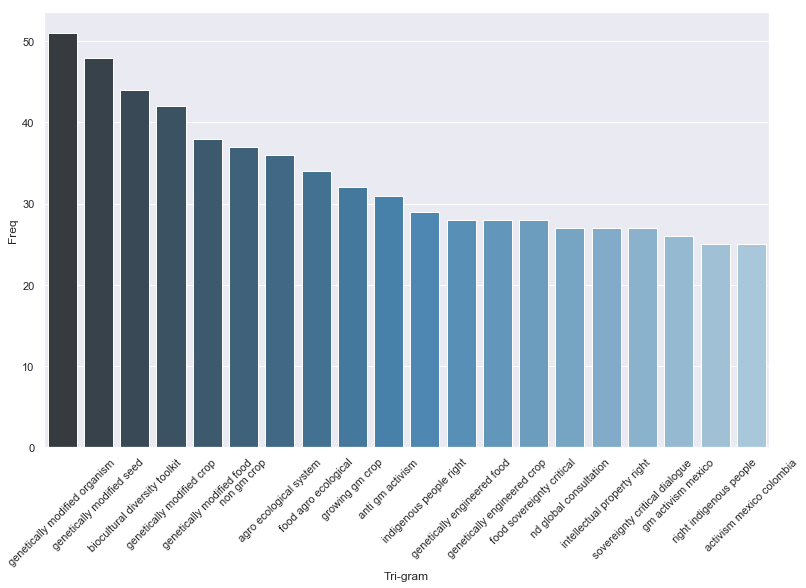
\includegraphics[width=14cm]{Figures/bar5.png}
\end{figure}

\textbf{Code: Tri-grams (pro-GM)}

\begin{lstlisting}
#Most frequently occurring Tri-grams
top3_wordsPRO = get_top_n3_words(corpus_pro, n=20)
top3_dfPRO = pandas.DataFrame(top3_wordsPRO)
top3_dfPRO.columns=["Tri-gram", "Freq"]
print(top3_dfPRO)
#Barplot of most freq Tri-grams
import seaborn as sns
sns.set(rc={'figure.figsize':(13,8)})
j=sns.barplot(x="Tri-gram", y="Freq", data=top3_dfPRO, palette="Blues_d")
j.set_xticklabels(j.get_xticklabels(), rotation=45)
\end{lstlisting}

\textbf{Output: Tri-grams (pro-GM)}

\begin{table}[H]
\begin{footnotesize}
\begin{tabular}{lll}
0  & pg economics ltd             & 199 \\
1  & gm crop impact               & 198 \\
2  & gm ht soybean                & 139 \\
3  & field eiq ha                 & 99 \\
4  & gm ir cotton                 & 95 \\
5  & genetically engineered crop  & 71 \\
6  & using gm ht                  & 71 \\
7  & impact using gm              & 69 \\
8  & farm income gain             & 65 \\
9  & national academy science     & 63 \\
10 & gm ir maize                  & 61 \\
11 & kg carbon ha                 & 61 \\
12 & farm income benefit          & 58 \\
13 & academy science engineering  & 54 \\
14 & science engineering medicine & 54 \\
15 & income impact using          & 53 \\
16 & carbon ha year               & 52 \\
17 & gm ht maize                  & 51 \\
18 & genetically modified crop    & 49 \\
19 & national academy press       & 49 \\
\end{tabular}
\end{footnotesize}
\end{table}


\begin{figure}[H]
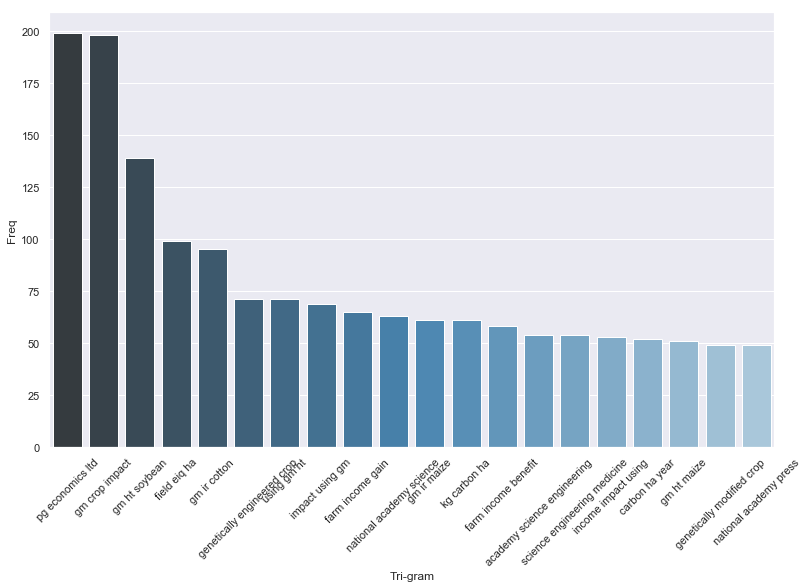
\includegraphics[width=14cm]{Figures/bar6.png}
\end{figure}

\section{Type-Token Ratio}
Lexical diversity is calculated through the type-token ratio (TTR). For this, the non-preprocessed texts were used so TTR values could be compared with other corpora/texts.

\textbf{Code: TTR}

\begin{lstlisting}
antiList = " ".join(anti_lines).split()
proList = " ".join(pro_lines).split()
# Yield successive n-sized 
# chunks from l. 
def divide_chunks(l, n): 
    # looping till length l 
        for i in range(0, len(l), n): 
            yield l[i:i + n] 
# n = how many elements in each list 
n = 2000
x = list(divide_chunks(antiList, n)) 
y = list(divide_chunks(proList, n)) 
TTRs = []
for chunk in x:
    wordsUnique = []
    for word in chunk:
        if word not in wordsUnique:
            wordsUnique.append(word)
    ttr=len(wordsUnique)/len(chunk)
    TTRs.append(ttr)
TTRsPro = []
for chunk in y:
    wordsUnique = []
    for word in chunk:
        if word not in wordsUnique:
            wordsUnique.append(word)
    ttr=len(wordsUnique)/len(chunk)
    TTRsPro.append(ttr)
antiLD = sum(TTRs) / len(TTRs)
proLD = sum(TTRsPro) / len(TTRsPro)
print("anti-GM Corpus: " + str(round(antiLD,2)))
print("pro-GM Corpus:  " + str(round(proLD,2)))
\end{lstlisting}

\textbf{Output: TTR for each subcorpus}

\begin{footnotesize}
anti-GM Corpus: 0.45\newline
pro-GM Corpus:  0.42
\end{footnotesize}

\section{Specialized Terminology}
A more direct measure of the presence of scientific terminology is comparison of the corpora with a dictionary of scientific terms. To conduct such a comparison, a molecular biology glossary is used which comprised of 170 terms. For each subcorpora, counts were taken for the frequency of glossary terms. 

To account for the different sizes of corpora, frequencies are based on a random sample of 100,000 tokens from each corpus. The average frequency was then calculated over 100 random samples.

For each corpus we output the counts (e.g., {gene:445}) to determine precisely which molecular biology terms appeared in each subcorpus. 

\textbf{Code: Specialized Terms}

\begin{lstlisting}
import random
from collections import Counter
f= open("...allTerms.txt", "r", encoding="UTF-8")
terms = f.readlines()
allTerms = [x.lower() for x in terms]
allTerms= [x.replace('\n', '') for x in allTerms]
print(str(len(terms)) + " terms in the dictionary\n") 
from random import sample
print("Random sample of terms:")
chose_terms = sample(terms, 3)
for i in chose_terms:
    print("-"+i[0:-1])
print("\n")
subList = []
counts_anti = []
counts_pro = []
words_anti = []
words_pro = []
size=100000
print("taking " + str(10)+ " samples of " +str(size) + " tokens..." + "\n")
def getCount(corpus, lst, words):
    for y in allTerms:
        if corpus.count(y) > 1:
            subList.append(y)
    samples = []
    i=0
    while i < 10:
        sampleRand=random.sample(corpus.split(), size)
        samples.append(sampleRand)
        i=i+1
    for sample in samples:
        count=0
        for z in subList:
            for q in sample:
                if z==q:
                    count=count+1
                    words.append(z)
        lst.append(count)
getCount(anti_textPre, counts_anti, words_anti)    
getCount(pro_textPre, counts_pro, words_pro)    
average = sum(counts_anti)/len(samples)
average_pro = sum(counts_pro)/len(samples)
print("average frequency (anti-GM): " +str(round(average,10)))
print("average frequency (pro-GM): " +str(round(average_pro,10)))
d1 = dict()
for i in words_anti:
  d1[i] = d1.get(i, 0) + 1
d2 = dict()
for i in words_pro:
  d2[i] = d2.get(i, 0) + 1
import operator
sorted_d1 = sorted(d1.items(), key=operator.itemgetter(1), reverse=True)
sorted_d2 = sorted(d2.items(), key=operator.itemgetter(1), reverse=True)
print("\n" + "Terms in the anti-GM corpus:")
print(sorted_d1)
print("\n" + "Terms in the pro-GM corpus:")
print(sorted_d2)
\end{lstlisting}

\textbf{Output: Specialized Terms (Molecular Biology)}
\begin{footnotesize}

170 terms in the dictionary

Random sample of terms:\newline
-Anneal\newline
-BAC\newline
-Acrylamide gels

taking 10 samples of 100000 tokens...

average frequency (anti-GM): 101.7\newline
average frequency (pro-GM): 439.0

Terms in the anti-GM corpus:
[('gene', 477), ('expression', 99), ('genome', 87), ('hybridization', 66), ('processing', 54), ('message', 35), ('insert', 34), ('restriction', 34), ('sequence', 25), ('marker', 23), ('library', 16), ('primer', 13), ('promoter', 13), ('translation', 13), ('cap', 9), ('nt', 8), ('plasmid', 6), ('genotype', 5)]

Terms in the pro-GM corpus:
[('nt', 2334), ('gene', 1234), ('genome', 228), ('sequence', 128), ('expression', 124), ('processing', 94), ('cap', 90), ('message', 46), ('insert', 40), ('marker', 32), ('lambda', 10), ('screening', 10), ('hybridization', 7), ('library', 7), ('promoter', 6)]
\end{footnotesize}

\textbf{Code: Concondance lines of \textit{NT}}

The output above suggests that the pro-GM corpus has over 4 times the number of terms. However, from the output counts we see that 'NT' (abbr. for nucleotide) is disproportionate in the pro-GM corpus. To investigate we look at the context of where 'NT' appears in the text.

Below we take a random sample of concordances of 'NT'. We see that is not used as an abbreviation for nucleotide; rather, it NT means frequently means no-till in this corpus. Moreover, we see that there are only 128 matches, far fewer than indicated in the counts above. This means that 'nt' (as a lowercase substring) was counted above where is had little to do with 'NT' meaning nucleotide.
\newline
\begin{lstlisting}
nt_concord = []
for i in range(0,len(proList)):
    if proList[i] == "NT":
        snippet = " ".join(proList[i-15:i+15])
        loc = snippet.index("NT")
        line = snippet[loc-25:loc+32]
        if line not in nt_concord:
            nt_concord.append(line)
print("count:" +str(len(nt_concord))+ "\n")
print('Random sample:' ) 
from random import sample
chosen_nt = sample(nt_concord, 10)
for i in chosen_nt:
    print(i)
\end{lstlisting}

\textbf{Output: Concondance lines of \textit{NT}}

\begin{footnotesize}
count:128

Random sample:

relating to the use of NT systems 111) and this identif\newline
\ \ ith the premise that NT results in positive carbon se\newline
.......... systems. The NT system stored and retained 7.\newline
\ area is in continuous NT crop rotation, the full SOC b\newline
estimated that RT or NT typically uses 19 to 38 litre\newline
been by farmers using NT systems (GM HT cultivars acco\newline
8) work also compared NT and full-inversion tillage (F\newline
Mathew et al. (2012)). NT soils are more biologically a\newline
014 Total Assumption: NT = +175 kg carbon/ha/yr, CT = \newline
rch comparing CT with NT has demonstrated that NT resu\newline
\end{footnotesize}

\textbf{Code: Terms (Molecular Biology) - Adjusted}

\begin{lstlisting}
allTerms.remove('nt')
subList = []
counts_anti = []
counts_pro = []
words_anti = []
words_pro = []
getCount(anti_textPre, counts_anti, words_anti)    
getCount(pro_textPre, counts_pro, words_pro)
average = sum(counts_anti)/len(samples)
average_pro = sum(counts_pro)/len(samples)
print("Results after removing 'NT' from the terms:\n")   
print("average frequency (anti-GM): " +str(round(average,10)))
print("average frequency (pro-GM): " +str(round(average_pro,10)))
\end{lstlisting}

\textbf{Output: Terms (Molecular Biology) - Adjusted}

\begin{footnotesize}
Results after removing 'NT' from the terms:

average frequency (anti-GM): 79.3\newline
average frequency (pro-GM): 205.6
\end{footnotesize}

\textbf{Code: Terms (Agrochemicals)}

The same dictionary process was repeated with a glossary of agrochemicals. Common names of 2,498 herbicides and pesticides were collected and frequencies obtained for both subcorpora.

\begin{lstlisting}
g= open("...herbPestNames.txt", "r", encoding="UTF-8")
termsHerb = g.readlines()
allTerms = [x.lower() for x in termsHerb]
allTerms= [x.replace('\n', '') for x in allTerms]
print(str(len(termsHerb)) + " terms in the dictionary\n") 
from random import sample
print("Random sample of terms:")
chose_termsHerb = sample(termsHerb, 3)
for i in chose_termsHerb:
    print("-"+i[0:-1])
print("\n")
subList = []
counts_anti = []
counts_pro = []
words_anti = []
words_pro = []
size=100000
print("taking " + str(10)+ " samples of " +str(size) + " tokens..." + "\n")
getCount(anti_textPre, counts_anti, words_anti)    
getCount(pro_textPre, counts_pro, words_pro)
average = sum(counts_anti)/len(samples)
average_pro = sum(counts_pro)/len(samples)
print("average frequency (anti-GM): " +str(round(average,10)))
print("average frequency (pro-GM): " +str(round(average_pro,10)))
d1 = dict()
for i in words_anti:
  d1[i] = d1.get(i, 0) + 1
d2 = dict()
for i in words_pro:
  d2[i] = d2.get(i, 0) + 1
import operator
sorted_d1 = sorted(d1.items(), key=operator.itemgetter(1), reverse=True)
sorted_d2 = sorted(d2.items(), key=operator.itemgetter(1), reverse=True)
print("\n" + "Terms in the anti-GM corpus:")
print(sorted_d1)
print("\n" + "Terms in the pro-GM corpus:")
print(sorted_d2)
\end{lstlisting}

\textbf{Output: Terms (Agrochemicals)}

\begin{footnotesize}

2498 terms in the dictionary

Random sample of terms:\newline
-proparthrin\newline
-cicloheximide\newline
-jasmolin II

taking 10 samples of 100000 tokens...

average frequency (anti-GM): 91.9\newline
average frequency (pro-GM): 595.6

Terms in the anti-GM corpus:\newline
[('glyphosate', 710), ('glufosinate', 102), ('dicamba', 32), ('paraquat', 22), ('atrazine', 22), ('ddt', 21), ('dep', 10)]

Terms in the pro-GM corpus:\newline
[('glyphosate', 3744), ('glufosinate', 660), ('atrazine', 232), ('clethodim', 138), ('fomesafen', 114), ('chlorimuron', 102), ('flumioxazin', 100), ('trifluralin', 96), ('acetochlor', 80), ('pendimethalin', 64), ('prometryn', 58), ('dicamba', 52), ('sulfentrazone', 50), ('metolachlor', 39), ('imazethapyr', 36), ('metsulfuron', 36), ('imidacloprid', 35), ('diuron', 32), ('cypermethrin', 31), ('methomyl', 30), ('acetamiprid', 26), ('chlorpyrifos', 26), ('acc', 26), ('diafenthiuron', 17), ('deltamethrin', 16), ('buprofezin', 14), ('acephate', 12), ('endosulfan', 12), ('phoxim', 12), ('abamectin', 12), ('metaflumizone', 11), ('parathion', 11), ('cyhalothrin', 10), ('monocrotophos', 9), ('chlorfenapyr', 7), ('cma', 6)]

\end{footnotesize}

\section{Concordances of \textit{ecological} \& \textit{biological}}
Concordances of the words \textit{ecological} and \textit{biological} can provide insight into how living systems are referred to linguistically. 

\textbf{Code: Concordances of \textit{ecological}}

\begin{lstlisting}
anti_low = anti_text.lower()
anti_list = anti_low.split()
culture_concord = []
for i in range(0,len(anti_list)):
    if anti_list[i] == "culture":
        snippet = " ".join(anti_list[i-15:i+15])
        loc = snippet.index("culture")
        line = snippet[loc-25:loc+32]
        if line not in culture_concord:
            culture_concord.append(line)
print('ANTI-GM Corpus' + "\n--------------" + "\n")             
print("Total unqiue lines: " + str(len(culture_concord)) + "\n")
print('Random sample:' + "\n") 
from random import sample
chosen_cult = sample(culture_concord, 10)
for i in chosen_cult:
    print(i)
pro_low = pro_text.lower()
pro_list = pro_low.split()
culture_concord_pro = []
for i in range(0,len(pro_list)):
    if pro_list[i] == "culture":
        snippet = " ".join(pro_list[i-15:i+15])
        loc = snippet.index("culture")
        line = snippet[loc-25:loc+32]
        if line not in culture_concord_pro:
            culture_concord_pro.append(line)
print('\nPRO-GM Corpus' + "\n--------------" + "\n")            
print("Total unqiue lines: " + str(len(culture_concord_pro)) + "\n")
for i in culture_concord_pro:
    print(i)
\end{lstlisting}

\textbf{Output: Concordances of \textit{ecological}}

\begin{footnotesize}
ANTI-GM Corpus\newline
-----------------------

Total unique lines: 107

Random sample:

g role culture food agro ecological system sound alert po\newline
tion meet need community ecological refugia pastoral netw\newline
ustomary law traditional ecological knowledge legal frame\newline
pacific northwest social ecological system ecology societ\newline
challenge coupled social ecological system address challe\newline
ge traditional food agro ecological system number differe\newline
ay france gmos demanding ecological approach agriculture \newline
shock like flood drought ecological farming model based b\newline
igenous people food agro ecological system indigenous peo\newline
on feeding volatile city ecological sustainability subsis\newline
ing haiti cannot sustain ecological destruction impositio\newline
m assessment traditional ecological knowledge zerner godo\newline
nsidered necessary sound ecological management riddell ec\newline
ell song dance myth agro ecological food system offer sig

PRO-GM Corpus\newline
-----------------------

Total unique lines: 14

edness combined volatile ecological climate socioeconomic\newline
tton htm shetty pk socio ecological implication pesticide\newline
 industrial biotech agro ecological paradigm drawing aspe\newline
 different crop one many ecological farming practice us k\newline
g people real food based ecological agriculture address m\newline
esting climate resilient ecological agriculture empowerin\newline
 sheet describing health ecological environmental effect \newline
onent consumer component ecological component component e\newline
age farm worker consumer ecological component eiq c dt dt\newline
e ability absorbed plant ecological component model compo\newline
ion farm worker consumer ecological average eiq value pre\newline
et al assessing economic ecological impact herbicide tole\newline
hed march concluded agro ecological farming system feed w
\end{footnotesize}

\textbf{Code: Concordances of \textit{biological}}

\begin{lstlisting}
getConcord("biological", bio_concord, bio_concord_pro)
print('ANTI-GM Corpus' + "\n--------------" + "\n")             
print("Total unique lines: " + str(len(bio_concord)) + "\n")
print('Random sample:' + "\n") 
from random import sample
chosen_bio = sample(bio_concord, 10)
for i in chosen_bio:
    print(i)
pro_low = pro_text.lower()
pro_list = pro_low.split()
print('\nPRO-GM Corpus' + "\n--------------" + "\n")            
print("Total unique lines: " + str(len(bio_concord_pro)) + "\n")
for i in bio_concord_pro:
    print(i)
\end{lstlisting}

\textbf{Output: Concordances of \textit{biological}}

\begin{footnotesize}

ANTI-GM Corpus\newline
-----------------------

Total unique lines: 94

Random sample:

rge share world cultural biological diversity yet largely\newline
y human culture language biological cultural linguistic b\newline
tal knowledge convention biological diversity hlclep firs\newline
or due instance chemical biological function kill growing\newline
ranking position country biological language diversity co\newline
ndigenous culture people biological productive resource s\newline
ervation sustainable use biological diversity promote wid\newline
used organic farmer form biological pest control crop gen\newline
ference party convention biological diversity prepared dr\newline
mmunication need however biological specie human language

PRO-GM Corpus\newline
-----------------------

Total unique lines: 10

sustainable modification biological resource going much p\newline
 really dad arguing need biological solution like gm redu\newline
truction expand research biological science based program\newline
enta innovative chemical biological solution aligning new\newline
peed automated synthesis biological method prepare quanti\newline
 change plant metabolism biological activity complex regi\newline
anic farmer e g new type biological control tested decade\newline
 country use alternative biological cultural control meas\newline
examination data diverse biological societal aspect curre\newline
arch study found adverse biological social effect ge crop
\end{footnotesize}

\textbf{Code: Concordances of \textit{culture}}

\begin{lstlisting}
culture_concord = []
culture_concord_pro = []
getConcord("culture", culture_concord, culture_concord_pro)
print('ANTI-GM Corpus' + "\n--------------" + "\n")             
print("Total unique lines: " + str(len(culture_concord)) + "\n")
print('Random sample:' + "\n") 
from random import sample
chosen_culture = sample(culture_concord, 10)
for i in chosen_culture:
    print(i)
pro_low = pro_text.lower()
pro_list = pro_low.split()
print('\nPRO-GM Corpus' + "\n--------------" + "\n")            
print("Total unique lines: " + str(len(culture_concord_pro)) + "\n")
for i in culture_concord_pro:
    print(i)
\end{lstlisting}

\textbf{Output: Concordances of \textit{culture}}

\begin{footnotesize}

ANTI-GM Corpus\newline
-----------------------

Total unique lines: 211

Random sample:

ation science technology culture including seed medicine\newline 
nt emphasizes importance culture needed value identified\newline
 world difference nature culture benefit human life yet m\newline
 people without language culture cannot survive assembly\newline 
edge connection language culture environment local level\newline 
 corn core rural mexican culture millennium every ground\newline 
able training accordance culture order achieve technical\newline 
g deemed legal done harm culture community gmos different\newline
t recognition importance culture development un education\newline
 acceptable within given culture accessibility food way s

PRO-GM Corpus\newline
-----------------------

Total unique lines: 4

gy seed teach farmer new culture practice get completely\newline
op tool including tissue culture diagnostics genomics mol\newline
formed cell grown tissue culture become plantlet eventual\newline
icroorganism e g starter culture changed precisely random
\end{footnotesize}


\textbf{Code: Concordances of \textit{culture}}

\begin{lstlisting}
indig_concord = []
indig_concord_pro = []
getConcord("indigenous", indig_concord, indig_concord_pro)
print('ANTI-GM Corpus' + "\n--------------" + "\n")                     
print("Total unique lines: " + str(len(indig_concord)) + "\n")
print('Random sample:' + "\n") 
from random import sample
chosen_indig = sample(indig_concord, 10)
for i in chosen_indig:
    print(i)
pro_low = pro_text.lower()
pro_list = pro_low.split()
print('\nPRO-GM Corpus' + "\n--------------" + "\n")            
print("Total unique lines: " + str(len(indig_concord_pro)) + "\n")
for i in indig_concord_pro:
    print(i)
\end{lstlisting}

\textbf{Output: Concordances of \textit{indigenous}}

\begin{footnotesize}

ANTI-GM Corpus\newline
-----------------------

Total unique lines: 784

Random sample:

deral level exist mexico indigenous population living wit\newline
support system mean many indigenous migrant live distress\newline
uld undermine livelihood indigenous people genetic use re\newline
y program restrict limit indigenous people use access lan\newline
n implemented adequately indigenous people adopted vote f\newline
meet cultural aspiration indigenous people livestock rais\newline
g common property regime indigenous local community terri\newline
subsistence food carried indigenous people percentage tra\newline
ce however effect factor indigenous people role indigenou\newline
ecognized un declaration indigenous people rarely consult

PRO-GM Corpus\newline
-----------------------

Total unique lines: 0

\end{footnotesize}


\section{Distribution of Geographic Entities}
Some quantitative analysis provides a better view concentration and distribution of countries in the corpus. Using the Python software package \textit{geotext} country and city names are extracted from each subcorpus. City names are counted only if the population is greater than 500,000. The cities are then referenced back to their countries and the resulting countries are counted and sorted for each subcorpus.

\textbf{Code: Countries in the Corpus}

\begin{lstlisting}
# import libraries for entity recognition and country codes
import sys
from geotext import GeoText
from iso3166 import countries
from tabulate import tabulate
# read corpus and data
anti_file = "...\anti_gmo.txt"
pro_file = "...\pro_gmo.txt"
cities_file = "...worldcities.csv"
# create lists as global 
freqMaster = {}
freq_anti = {} 
freq_pro = {} 
freqCities_anti = {}
freqCities_pro = {}
countByCit_anti = []
countByCit_pro = []
# define function
def geo(corpusFile, targList, wc, freq, freqCities):
    with open (corpusFile, "r", encoding="utf8") as f:
        lines = f.readlines()
        text=" ".join(lines)
        wordCount = len(text.split())/1000
        wc.append(wordCount)
        # get reference list of all country names (iso3166)
        refList = []
        for c in countries:
            refList.append(c[-1])
        # get countries and cities from corpus 
        places = GeoText(text)
        countriesAll = places.countries
        citiesAll = places.cities
        # import cities to cross-reference
        import pandas
        colnames = ["city","city_ascii","lat","lng","country","iso2","iso3",
        "admin_name","capital","population","id"]
        data = pandas.read_csv(cities_file, names=colnames)
        names = data.city.tolist()
        country = data.country.tolist()
        population = data.population.tolist()
        countriesByCities = []
        for city in citiesAll:
            if city in names:
                ind=names.index(city)
                if float(population[ind]) > 500000:
                    #print(names[ind] + "," + " " + country[ind] +"," + " " +
                    str(population[ind]))
                    countriesByCities.append(country[ind])
        # custom replace country names of with iso3166
        countriesAll = ["Bolivia, Plurinational State of" if x=="Bolivia" 
        else x for x in countriesAll]
        countriesAll = ["United States of America" if x=="United States" 
        else x for x in countriesAll]
        countriesByCities = ["United States of America" if x=="United States" 
        else x for x in countriesByCities]
        countriesAll = ["Tanzania, United Republic of" if x=="Tanzania" 
        else x for x in countriesAll]
        countriesAll = ["Venezuela, Bolivarian Republic of" if x=="Venezuela" 
        else x for x in countriesAll]
        countriesByCities = ["Venezuela, Bolivarian Republic of" if x=="Venezuela"
         else x for x in countriesByCities]
        countriesAll = ["Viet Nam" if x=="Vietnam" else x for x in countriesAll]
        countriesAll = ["Syrian Arab Republic" if x=="Syria" 
        else x for x in countriesAll]
        countriesAll = ["United Kingdom of Great Britain and Northern Ireland" 
        if x=="United Kingdom" else x for x in countriesAll]
        countriesByCities = ["United Kingdom of Great Britain and Northern Ireland"
        if x=="United Kingdom" else x for x in countriesByCities]
        countriesAll = ["Korea, Republic of" if x=="South Korea" 
        else x for x in countriesAll]
        countriesAll = ["Czechia" if x=="Czech Republic" else x for x in countriesAll]
        countriesAll = ["Russian Federation" if x=="Russia" else x for x in countriesAll]
        countriesAll = ["Micronesia, Federated States of" if x=="Micronesia" 
        else x for x in countriesAll]
        if "Vatican" in countriesAll:
            countriesAll.remove("Vatican")
        # find country names in the corpus that do not correspond to an iso3166 name
        # print any suggestions for custom name replace
        noFits = []
        for x in countriesAll:
            if x not in refList:
                if x not in noFits:
                    noFits.append(x)
        if len(noFits)>0:
            print("No country code found for: ")
            for x in noFits:
                print(x)
        for x in noFits:
            for y in refList:
                if x in y:
                    print("try: " + y)
        # create dict with country counts {"CAN":23, USA:89, ...} 
        # dict for both country mentions and city mentions
        for c in countriesAll: 
            item = countries.get(c)[2]
            if (item in freq): 
                freq[item] += 1
            else: 
                freq[item] = 1
            if (item in freqMaster): 
                freqMaster[item] += 1
            else: 
                freqMaster[item] = 1
        for c in countriesByCities: 
            item = countries.get(c)[2]
            if (item in freqCities): 
                freqCities[item] += 1
            else: 
                freqCities[item] = 1
            if (item in freqMaster): 
                freqMaster[item] += 1
            else: 
                freqMaster[item] = 1
        tab = []
        sorted_freqMaster = sorted(freqMaster.items(), 
        key=operator.itemgetter(1), reverse=True)
        for key, value in sorted_freqMaster[0:10]:
            tab.append([countries.get(key)[0], round(value/wc[0],2)]])
        print(tabulate(tab, headers=['Country', 'Freq.']))
        for i in countriesByCities:
            targList.append(i)
print('ANTI-GM Corpus' + "\n")   
geo(anti_file, countByCit_anti, wc_anti, freq_anti, freqCities_anti)
print("\n"+'PRO-GM Corpus' + "\n")   
geo(pro_file, countByCit_pro, wc_pro, freq_pro, freqCities_pro)
\end{lstlisting}

\textbf{Output: Countries in the Corpus}

\begin{footnotesize}
ANTI-GM Corpus\newline
-----------------------

\begin{table}[H]
\begin{footnotesize}
\begin{tabular}{ll}

\textbf{Country}         & \textbf{Freq.} \\
Mexico                   & 0.82            \\
United States of America & 0.70           \\
Canada                   & 0.45           \\
India                    & 0.39           \\
Colombia                 & 0.30           \\
Nepal                    & 0.28           \\
Argentina                & 0.27           \\
Haiti                    & 0.25           \\
Brazil                   & 0.20           \\
Guatemala                & 0.17

\end{tabular}
\end{footnotesize}
\end{table}

PRO-GM Corpus\newline
-----------------------

\begin{table}[H]
\begin{footnotesize}
\begin{tabular}{ll}

\textbf{Country}         & \textbf{Freq.} \\
Argentina                & 1.04            \\
Canada                   & 0.91           \\
United States of America & 0.77            \\
Brazil                   & 0.67            \\
India                    & 0.60           \\
Australia                & 0.39           \\
South Africa             & 0.38           \\
Mexico                   & 0.34           \\
China                    & 0.32            \\
Philippines              & 0.29

\end{tabular}
\end{footnotesize}
\end{table}

\end{footnotesize}


\textbf{Code: North/South Geographic Split}

\begin{lstlisting}
import country_converter as cc
def nsSplit(freq, wc, freqCities, countByCit):
    cont = cc.convert(names = countByCit, to = 'UNregion')
    globNorth = 0
    globSouth = 0
    for c in cont:
        if c=="Northern America" or "Europe" in c:
            globNorth=globNorth+1
        else:
            globSouth=globSouth+1
    tab = []
    tab.append([round(100*globNorth/len(cont),2), round(100*globSouth/len(cont),2)])
    print(tabulate(tab, headers=['North (%)', 'South (%)']))
    ## get variation coefficient ##
    import statistics 
    # calculating deviation and variance
    sample = [] 
    countryFreqs = freq.values()
    for i in countryFreqs:
        sample.append(i/wc[0])
    mean = sum(sample)/len(sample)
    stdev = statistics.stdev(sample)
    coeff =stdev/mean
    # Prints standard deviation 
    # xbar is set to default value of 1 
    stddev = statistics.stdev(sample)
    print("\n"+"For the countries: ")
    print("Standard Deviation is % s " % (round(stddev,2))) 
    print("The coefficient of variation (CV) is " +  str(round(coeff,2)) +  "\n") 
    sample2 = [] 
    cityFreqs = freqCities.values()
    for i in cityFreqs:
        sample2.append(i/wc[0])
    mean2 = sum(sample2)/len(sample2)
    stdev2 = statistics.stdev(sample2)
    coeff2=stdev2/mean2
print('ANTI-GM Corpus' + "\n")       
nsSplit(freq_anti, wc_anti, freqCities_anti, countByCit_anti)
print('\nPRO-GM Corpus' + "\n")       
nsSplit(freq_pro, wc_pro, freqCities_pro, countByCit_pro)
\end{lstlisting}

\textbf{Output: North/South Geographic Split}

\begin{footnotesize}

ANTI-GM Corpus

\begin{table}[h]
\begin{footnotesize}
\begin{tabular}{ll}
\textbf{North (\%)} & \textbf{South (\%)} \\
61.99              & 38.01             
\end{tabular}
\end{footnotesize}
\end{table}

Standard Deviation is 0.12 \newline
The coefficient of variation (CV) is 1.87

PRO-GM Corpus

\begin{table}[h]
\begin{footnotesize}
\begin{tabular}{ll}
\textbf{North (\%)} & \textbf{South (\%)} \\
87.39            & 12.61             
\end{tabular}
\end{footnotesize}
\end{table}

Standard Deviation is 0.21 \newline
The coefficient of variation (CV) is 1.75

\end{footnotesize}

\textbf{Code: Shannon's Diversity Index}

\begin{lstlisting}
## calculating diversity of data
def divers(freqCities, wc):
    countryFreqs = []
    for i in freqCities.values():
        countryFreqs.append(i/wc)
    sumFreqs=sum(countryFreqs)
    n=len(countryFreqs)
    #average=sum(countryFreqs)/len(countryFreqs)
    proportions=[]
    for i in countryFreqs:
        proportions.append(i/sumFreqs)
    #print(proportions)
    import math
    listofzeros = [0] * (195-len(proportions))
    calcs = []
    for p in proportions:
        calc = p*(math.log(p))
        calcs.append(calc)
    final=listofzeros+calcs
    H1=-1*sum(final)
    print(round(H1,2))
    E=H1/math.log(195)
    print(round(E,2))
print('ANTI-GM Corpus') 
divers(freqCities_anti,wc_anti[0]*1000)
print('\nPRO-GM Corpus') 
divers(freqCities_pro,wc_pro[0]*1000
\end{lstlisting}

\textbf{Output:  Shannon's Diversity Index}
\begin{footnotesize}


ANTI-GM Corpus\newline
2.61\newline
0.49

PRO-GM Corpus\newline
1.3\newline
0.25

\end{footnotesize}


\section{Temporal Horizons \& Historical Context}

\textbf{Code: Concordances of \textit{centur*}}

\begin{lstlisting}
anti_file = "...\anti_gmo.txt"
pro_file = ...\pro_gmo.txt"
centur_concord = []
centur_concord_pro = []
def getConcordWildcard(file, targTerm, c1):
    with open (file, "r", encoding="utf8") as f:
        lines = f.readlines()
        text=" ".join(lines)
        low = text.lower()
        listsp = low.split()
        for i in range(0,len(listsp)):
            if targTerm in listsp[i]:
                snippet = " ".join(listsp[i-15:i+15])
                loc = snippet.index(targTerm)
                line = snippet[loc-25:loc+32]
                if line not in c1:
                    c1.append(line)
getConcordWildcard(anti_file, 'centur', centur_concord)
print('ANTI-GM Corpus' + "\n--------------" + "\n")                     
print("Total unique lines: " + str(len(centur_concord)) + "\n")
for i in centur_concord:
    print(i)
getConcordWildcard(pro_file, 'centur', centur_concord_pro)
print('\nANTI-GM Corpus' + "\n--------------" + "\n")                     
print("Total unique lines: " + str(len(centur_concord_pro)) + "\n")
for i in centur_concord_pro:
    print(i)
\end{lstlisting}

\textbf{Output: Concordances of \textit{centur*}}
\begin{footnotesize}
ANTI-GM Corpus\newline
-----------------------

Total unique lines: 34

e been enriched over the centuries through the abundant b\newline
ict (spanish in the 16th century, expropriation of land i\newline
economies since the 16th century, they have retained exte\newline
hich are the products of centuries of deliberate breeding\newline
eations that encapsulate centuries of historical events a\newline
odels at the turn of the century: individual property mod\newline
nt in panama in the 21st century. bioscience 51: 389-398.\newline
e first half of the 20th century, seeds were overwhelming\newline
llion by the turn of the century and that almost 1 billio\newline
eceived in the last half century. sustainable agriculture\newline
 that have been used for centuries. no-till farming is pr\newline
lture over the course of centuries, europeans have found \newline
nineteenth and twentieth centuries in europe, the man-mad\newline
in it. in mid-nineteenth century america, the natural won\newline
. in the late nineteenth century, the preservation of unt\newline
nforced in the twentieth century through the ways that ea\newline
tices sustain. twentieth-century philosophy in central eu\newline
 motifs of the twentieth century — that technology by its\newline
st half of the twentieth century to exercise precaution a\newline
y had depended on it for centuries. therefore it was very\newline
rsity over the twentieth century. now,just nine crops com\newline
to local conditions over centuries). these were rejected \newline
eds from their crops for centuries is at stake (as gmo cr\newline
ans beginning in the 8th century. 3. the ideological pare\newline
s, “during the past five centuries, while our people have\newline
r the course of the 20th century, according to the fao, a\newline
r they are the result of centuries of traditional plant b\newline
oped throughout the 20th century owe their origin to publ\newline
users guide for the 21st century31 argue, such a mindset \newline
ser’s guide for the 21st century. harry n. abrams, inc. 3\newline
he beginning of the 20th century, the world has lost 90\%\newline
rsity over the twentieth century. now, just nine crops co\newline
ich emerged in sixteenth century europe. i prefer the com\newline
l mexico. in the late 19 century into the contemporary pe

PRO-GM Corpus\newline
-----------------------

Total unique lines: 9

erspectives for the 21st century. session 17. 497-499. qa\newline
obal) by the end of this century in 2100 – global food se\newline
techniques in eighteenth century britain that brought abo\newline
ited states reflect many centuries of plant modification \newline
70 and 100 percent by midcentury. in particular, the rapi\newline
ple by the middle of the century. in one of his most ambi\newline
n the middle of the 20th century are the main reason that\newline
at have been planted for centuries. doohan looks at them \newline
 human foods in the 21st century: a review. biotechnol. a
\end{footnotesize}

\textbf{Code: Years in the Corpus}

\begin{lstlisting}
from operator import itemgetter
from collections import defaultdict
yearsf = "...\xseries.csv"
def plot_timeline(dataset, **kwargs):
    outpath = kwargs.pop('savefig', None)  # Save the figure as an SVG
    colors  = kwargs.pop('colors', {})     # Plot the colors for the series.
    series  = set([])                      # Figure out the unique series
    # Bring the data into memory and sort
    dataset = sorted(list(dataset), key=itemgetter(0))
    # Make a first pass over the data to determine number of series, etc.
    for _, source, category in dataset:
        series.add(source)
        if category not in colors:
            colors[category] = 'k'
    # Sort and index the series
    series  = sorted(list(series))
    # Create the visualization
    x = []  # Scatterplot X values
    y = []  # Scatterplot Y Values
    c = []  # Scatterplot color values
    # Loop over the data a second time
    for timestamp, source, category in dataset:
        x.append(timestamp)
        y.append(series.index(source))
        c.append(colors[category])
    plt.figure(figsize=(16,6))
    plt.title(kwargs.get('title', "Years in the Corpus"))
    plt.ylim((-1,len(series)))
    plt.xlim((1800, dataset[-1][0]+10))
    plt.yticks(range(len(series)), series)
    plt.scatter(x, y, color=c, alpha=0.85, s=10)
    if outpath:
        return plt.savefig(outpath, format='svg', dpi=1600)
    return plt
if __name__ == '__main__':
    colors = {'red': 'r', 'blue': 'b', 'green': 'g'}
    with open(yearsf, 'r') as f:
        reader = csv.reader(f)
        plt = plot_timeline([
            (float(row[0]), row[1], row[2])
            for row in reader
        ], colors=colors)
        plt.show()
\end{lstlisting}

\textbf{Output: Years in the Corpus}
\begin{figure}[h]
\centering
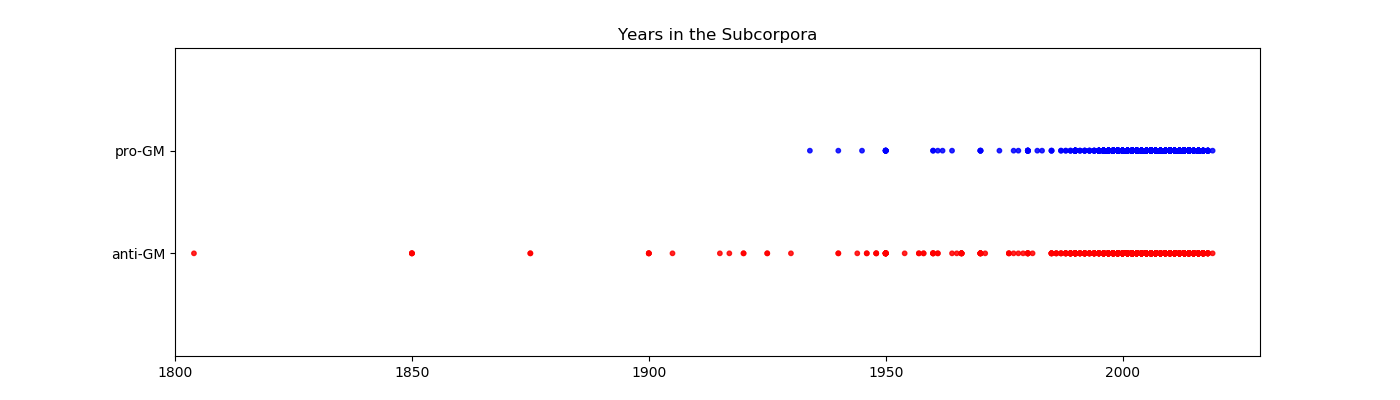
\includegraphics[width=16cm]{Figures/years.png}
\end{figure}

\section{Socio-Economic Context}

\textbf{Code: Concordances of \textit{income}}
\begin{lstlisting}
income_concord = []
income_concord_pro = []
getConcord("income", income_concord, income_concord_pro)
print('ANTI-GM Corpus' + "\n--------------" + "\n")                     
print("Total unique lines: " + str(len(income_concord)) + "\n")
print('Random sample:' + "\n") 
from random import sample
chosen_income = sample(income_concord, 10)
for i in chosen_income:
    print(i)
print('\nPRO-GM Corpus' + "\n--------------" + "\n")            
print("Total unique lines: " + str(len(income_concord_pro)) + "\n")
print('Random sample:' + "\n") 
from random import sample
chosen_income = sample(income_concord, 10)
for i in chosen_income:
    print(i)
\end{lstlisting}

\textbf{Output: Years in the Corpus}

\begin{footnotesize}

ANTI-GM Corpus\newline
--------------

Total unique lines: 58

Random sample:

y negative impact spread income farmer congress consideri\newline
ity rather lack adequate income access food country nativ\newline
hn resulted monsanto net income increasing million net in\newline
vailability access trade income generation purchasing foo\newline
 setting level necessary income also sought ensure farmer\newline
 rape sector canada lost income organic gm free producer \newline
 number household report income source outside community \newline
t climate change adapted income earning activity etc way \newline
ommodity price push farm income percent year billion lowe\newline
 bushel acre would meant income c end plant barley earned

PRO-GM Corpus\newline
--------------

Total unique lines: 237

Random sample:

ure livelihood outcome r income e increased wellr reduced\newline
overall effect crop farm income negative feedback farmer \newline
ity rather lack adequate income access food country nativ\newline
ience ht crop translated income benefit positive aspect i\newline
 agrochemical use farmer income look indirect impact deve\newline
rent indigenousgenerated income earning activity member a\newline
odity price pushing farm income expected lowest level six\newline
hn resulted monsanto net income increasing million net in\newline
vailability access trade income generation purchasing foo\newline
d reduce potential gross income sale fewer larger farm re

\end{footnotesize}

\textbf{Code: Collocates of \textit{corporate}}
\begin{lstlisting}
corporate_concord = []
corporate_concord_pro = []
corp_anti = []
corp_pro = []
getConcordWildcard(anti_file, 'corporate', corporate_concord) 
getConcordWildcard(pro_file, 'corporate', corporate_concord_pro) 
def getCorp(lst1, lst2):
    for i in lst1:
        if len(i) > 1:
            j=i.split()
            if("corporate" in j):
                ind = j.index("corporate")
                s = j[ind+1]
                s = re.sub(r'[^\w\s]','',s)
                lst2.append(s)
    d1a = dict()
    for i in lst2:
      d1a[i] = d1a.get(i, 0) + 1
    sorted_d1a = sorted(d1a.items(), key=operator.itemgetter(1), reverse=True)
    out = []
    for key, value in sorted_d1a:
        if value>1:
            out.append([key, value])
    print(tabulate(out, headers=['Collocate', 'Freq.']))
print('ANTI-GM Corpus:' + "\n")                     
print("Total unique lines: " + str(len(corporate_concord)) + "\n")
getCorp(corporate_concord, corp_anti)      
print('\nPRO-GM Corpus:' + "\n")            
print("Total unique lines: " + str(len(corporate_concord_pro)) + "\n")
getCorp(corporate_concord_pro, corp_pro) 
\end{lstlisting}

\textbf{Output: Collocates of \textit{corporate}}

\begin{footnotesize}
ANTI-GM Corpus:

Total unique lines: 87
\end{footnotesize}

\begin{table}[H]
\begin{footnotesize}
\begin{tabular}{ll}
\textbf{Collocate} & \textbf{Freq.} \\
sector             & 10             \\
control            & 8              \\
power              & 4              \\
seed               & 4              \\
agriculture        & 3              \\
sectors            & 2              \\
greed              & 2              \\
subsidies          & 2              \\
takeover           & 2              \\
consolidation      & 2             
\end{tabular}
\end{footnotesize}
\end{table}
\begin{footnotesize}
Pro-GM Corpus:

Total unique lines: 23
\end{footnotesize}

\begin{table}[H]
\begin{footnotesize}
\begin{tabular}{ll}
\textbf{Collocate} & \textbf{Freq.} \\
watch      & 2             
\end{tabular}
\end{footnotesize}
\end{table}


\textbf{Code: Income Split}

\begin{lstlisting}
gdp_file = "C:...\gdp.csv"
import pandas
colnames1 = ["rank","country","gdp"]
data_gdp = pandas.read_csv(gdp_file, names=colnames1)
rank_gdp = data_gdp["rank"].tolist()
countries_gdp = data_gdp["country"].tolist()
gdp = data_gdp["gdp"].tolist()
countries_gdp = [w.replace('\xa0', '') for w in countries_gdp]
ranks = dict(zip(countries_gdp, rank_gdp))
gdps = dict(zip(countries_gdp, gdp))
quart = int(0.25*len(countries_gdp))
quartile_top = countries_gdp[0:quart]
quartile_bottom = countries_gdp[2*quart:4*quart]
def sumRanks(dic, master):
    keysC = []
    valuesC = []
    countr = []
    sorted_dic = sorted(dic.items(), key=operator.itemgetter(1), reverse=True)
    for key, value in sorted_dic:
        keysC.append(countries.get(key)[0])
        valuesC.append(value)
        if countries.get(key)[0] not in countries_gdp:
            print(countries.get(key)[0])
    tot_dic = 0
    for c in master:
        tot_dic=tot_dic+int(ranks.get(c))
    print("avg rank: " + str(int(tot_dic/len(master))))
    tot_gdp = 0
    for c in master:
        #print(c)
        tot_gdp=tot_gdp+int(gdps.get(c))
    print("avg gdp " + str(round(tot_gdp/len(master),2)))
    count_top = 0
    count_bottom = 0
    for c in master:
        if c in quartile_top:
            count_top = count_top+1
        if c in quartile_bottom:
            count_bottom = count_bottom+1 
    print("% in top quartile: " + str(100*round(count_top/len(master),2)))
    print("% in bottom quartile: " + str(100*round(count_bottom/len(master),2)))
    #print(len(keysC))
print('ANTI-GM Corpus' + "\n")  
sumRanks(freq_anti, master_anti)
print("\n"+'PRO-GM Corpus' + "\n")  
sumRanks(freq_pro, master_pro)

\end{lstlisting}


\textbf{Output: Income Split}

\begin{footnotesize}
ANTI-GM Corpus

avg rank: 90\newline
avg GDP: 20765.94\newline
\% in top quartile: 32.0\newline
\% in bottom quartile: 38.0

PRO-GM Corpus

avg rank: 81\newline
avg GDP: 22370.72\newline
\% in top quartile: 35.0\newline
\% in bottom quartile: 32.0
\end{footnotesize} % Appendix A

\chapter{Appendix 2}
\lhead{\textit{Appendix 2}}
This appendix contains the data analysis (using Python) for the analysis described in Chapter 4. The data is a corpus consisting of articles and webpages covering the Dakota Access Pipeline (DAP). The data was collected manually using a search engine. Results were saved as separate txt files. 

Raw data is available in the folder \textit{Analysis 2} in a in a GitHub repo: \href{https://github.com/craigmateo/multilevel_corpus}{https://github.com/craigmateo/multilevel\_corpus}

The sections below contain a description of each analysis carried out as well as the corresponding Python code and the output from running that code. 

\section{Pre-processing}

The code below reads the 2 \textit{txt} files and does preprocessing on the text. The preprocessing consists of:

1. \textbf{Noise removal} (removal of punctuation, special characters, digits)
2. \textbf{Normalization} (stemming, lemmatization, removal of stopwords) 

Excerpts from the each preprocessed subcorpus are then printed.

\textbf{Code: Pre-processing}

\begin{lstlisting}
import pandas as pd
import glob
total=0
txt_files = glob.glob("C:...\\corpus\\*.txt")
raw_lines = []
#txt_files = glob.glob("*.txt")
for filename in txt_files:
	with open(filename, "r", encoding="utf-8") as f:
		x = f.readlines()
		for line in x:
			raw_lines.append(line)
# Libraries for text preprocessing
import re
import nltk
#nltk.download('stopwords')
from nltk.corpus import stopwords
from nltk.stem.porter import PorterStemmer
from nltk.tokenize import RegexpTokenizer
#nltk.download('wordnet') 
from nltk.stem.wordnet import WordNetLemmatizer
##Creating a list of stop words
stop_words = set(stopwords.words("english"))
corpus_PRE = []
corpus = []
for i in range(0, len(raw_lines)):
    #Remove punctuation
    #text = re.sub('[^a-zA-Z]', ' ', raw_lines[i])
    #remove tags
    text=re.sub("&lt;/?.*?&gt;"," &lt;&gt; ", raw_lines[i])
    #Convert to lowercase
    text = text.lower()
    # remove special characters and digits
    text=re.sub("(\\d|\\W)+"," ",text)
    corpus_PRE.append(text)
    ##Convert to list from string
    text = text.split()
    ##Stemming
    ps=PorterStemmer()
    #Lemmatisation
    lem = WordNetLemmatizer()
    text = [lem.lemmatize(word) for word in text if not word in  
            stop_words] 
    text = " ".join(text)
    corpus.append(text)
text = " ".join(corpus)
print("Excerpt:" + "\n\n" + text[1100:1200])
\end{lstlisting}


\textbf{Output: Text excerpt}

\begin{footnotesize}

Excerpt:
ric preservation asked army corp engineer conduct formal environmental impact assessment issue envir
\end{footnotesize}


\section{Word Count}
One count is taken with only noise removal and another with both noise removal and normalization.

\textbf{Code: Word Count}

\begin{lstlisting}
textPre = " ".join(corpus_PRE)
num_words_PRE = format(len(textPre.split()),",")
num_words = format(len(text.split()),",")
print("\n" + 'Noise Removal:' + "\n")  
print(str(num_words_PRE))
print("\n" + 'Noise Removal & Normalization:' + "\n")  
print(str(num_words))
\end{lstlisting}

\textbf{Output: Word Count}

\begin{footnotesize}

Noise Removal:
291,856

Noise Removal \& Normalization:
174,974

\end{footnotesize}






\section{Quotations}
Quotations are extracted from the corpus using regular expression matching. 500 characters before and after each quotation are also extracted so, for each quote, the context as well as the speaker could be identified.

\textbf{Code: Quotations}

\begin{lstlisting}
quotesList = []
quoteContext = []
total=0
raw_text = []
for line in raw_lines:
    raw_text.append(line)
alltext = " ".join(raw_text)
quotes = re.findall(r'"(.*?)"', alltext)
for i in quotes:
    ind = alltext.index(i)
    start=ind-500
    end=(ind+len(i))+100
    context=alltext[start:end]
    context = context.replace("\n","")
    quotesList.append(i)
    quoteContext.append([i,context])
    total=total+1
print("\n" + 'Total Quotations:' + "\n") 
print(total)
print("\n" + 'Sample of Quotation (with context below):' + "\n") 
print('"' + quotesList[0] + '"' +"\n")
print(quoteContext[0][1])
\end{lstlisting}

\textbf{Output: Quotations}

\begin{footnotesize}

Total Quotations:
1101

Sample of Quotation (with context below):

"reshaping the national conversation for any environmental project that would cross the Native American land."

ny in the Standing Rock tribe considered the pipeline and its intended crossing of the Missouri River to constitute a threat to the region's clean water and to ancient burial grounds. In April 2016, Standing Rock Sioux elder LaDonna Brave Bull Allard established a camp as a center for cultural preservation and spiritual resistance to the pipeline; over the summer the camp grew to thousands of people.  The protests drew considerable  national and international attention and have been said to be "reshaping the national conversation for any environmental project that would cross the Native American land."[5] The U.S. Army Corps of Engineers had conducted a limited review of the route and found no sign

\end{footnotesize}

\textbf{Code: Manual Cleaning}

The initial list of 1101 quotes was manually cleaned by removing noise and lines that were obviously not spoken quotations. Duplicates were also removed. The result was a list of 660 quotes.

\begin{lstlisting}
import pandas
colnames = ['QUOTE', 'REMOVE']
data = pandas.read_csv("C:...\\remove.csv", names=colnames)
quotes = data.QUOTE.tolist()
remove = data.REMOVE.tolist()
cleanQuotes = []
totalRemoved = 0
for q in quotes:
	ind = quotes.index(q)
	if remove[ind]!="X":
		if q not in cleanQuotes:
			cleanQuotes.append(q)
	else:
		totalRemoved=totalRemoved+1
print("Original number: " + str(len(quotes)))
print("Number removed: " + str(totalRemoved))
print("Final list (deduped): " +str(len(cleanQuotes)))
\end{lstlisting}

\textbf{Output: Manual Cleaning}

\begin{footnotesize}
Original number: 988

Number removed: 255

Final list (deduped): 660
\end{footnotesize}


\textbf{Code: Grouping}

The 660 quotes were then further reduced manually and qualitatively. Similar quotes (i.e. similar themes/speakers) were removed. Also very short or one-word quotes were generally removed. The 100 or so remaining quotes were then separated into one of three groups:

* Group A: proponents who either actively voices support for the pipeline (e.g., company representatives) or took a legal or institutional stand against the pipeline protesters (e.g., law enforcement)
* Group B: protesting opponents of the pipeline, most notably the affected Indigenous peoples, but also others who came to Standing Rock, North Dakota to voice opposition
* Group C: supporters and allies of protesters, such as NGOs and politicians who spoke out against the pipeline/in support of protesters

\begin{lstlisting}
colnames = ['Quote', 'Speaker','Group']
data = pandas.read_csv("C:...\\grouped.csv", names=colnames)
quotes = data.Quote.tolist()
speakers = data.Speaker.tolist()
groups = data.Group.tolist()
print("total quotes: " +str(len(quotes)-1))
data.head() 
\end{lstlisting}

\textbf{Output: Grouping}

\begin{footnotesize}
total quotes: 92

\begin{table}[H]
\resizebox{\textwidth}{!}{%
\begin{tabular}{|l|l|l|}
\hline
\textbf{Quote}                                    & \textbf{Speaker}                              & \textbf{Group} \\ \hline
Protesters' escalated unlawful behavior this w... & Morton County Sheriff's Department            & A              \\ \hline
...damage caused after protesters set numerous... & Morton County Sheriff's Department            & A              \\ \hline
[The police said the protesters had been] very... & Morton County Sheriff's Department            & A              \\ \hline
...multiple archaeological studies conducted w... & Kelcy Warren, CEO of Energy Transfer Partners & A              \\ \hline
\end{tabular}%
}
\end{table}
\end{footnotesize}


\section{Keywords}

\textbf{Code: Keywords}

\begin{lstlisting}
groupA = []
groupB = []
groupC = []
for i in range(0,len(quotes)):
    if groups[i]=="A":
        groupA.append(quotes[i])
    if groups[i]=="B":
        groupB.append(quotes[i])
    if groups[i]=="C":
        groupC.append(quotes[i])
def process(group):
    post = []
    for i in range(0, len(group)):
        #Remove punctuation
        text = re.sub('[^a-zA-Z]', ' ', group[i])
        #Convert to lowercase
        text = text.lower()
        #remove tags
        text=re.sub("&lt;/?.*?&gt;"," &lt;&gt; ",text)
        # remove special characters and digits
        text=re.sub("(\\d|\\W)+"," ",text)
        ##Convert to list from string
        text = text.split()
        ##Stemming
        ps=PorterStemmer()
        #Lemmatisation
        lem = WordNetLemmatizer()
        text = [lem.lemmatize(word) for word in text if not word in  
                stop_words] 
        text = " ".join(text)
        post.append(text)
    group.append(post)
process(groupA)
process(groupB)
process(groupC)
from sklearn.feature_extraction.text import CountVectorizer
import re
cv=CountVectorizer(max_df=0.8,stop_words=stop_words, max_features=10000, ngram_range=(1,3))
X=cv.fit_transform(groupA[-1])
list(cv.vocabulary_.keys())[:10]
#Most frequently occurring words
def get_top_n_words(corpus, n=None):
    vec = CountVectorizer().fit(corpus)
    bag_of_words = vec.transform(corpus)
    sum_words = bag_of_words.sum(axis=0) 
    words_freq = [(word, sum_words[0, idx]) for word, idx in      
                   vec.vocabulary_.items()]
    words_freq =sorted(words_freq, key = lambda x: x[1], 
                       reverse=True)
    return words_freq[:n]
#Convert most freq words to dataframe for plotting bar plot
top_wordsA = get_top_n_words(groupA[-1], n=20)
top_wordsB = get_top_n_words(groupB[-1], n=20)
top_wordsC = get_top_n_words(groupC[-1], n=20)
top_dfA = pandas.DataFrame(top_wordsA)
top_dfA.columns=["Word", "Freq"]
top_dfB = pandas.DataFrame(top_wordsB)
top_dfB.columns=["Word", "Freq"]
top_dfC = pandas.DataFrame(top_wordsC)
top_dfC.columns=["Word", "Freq"]
print("\n Group A \n")
print(top_dfA)
print("\n Group B \n")
print(top_dfB)
print("\n Group C \n")
print(top_dfC)
\end{lstlisting}

\textbf{Output: Manual Cleaning}

\begin{footnotesize}


\begin{table}[H]
\begin{tabular}{|l|l|l|l|l|l|}
\hline
\multicolumn{2}{|l|}{\textbf{Group A}}           & \multicolumn{2}{l|}{\textbf{Group B}}            & \multicolumn{2}{l|}{\textbf{Group C}}            \\ \hline
\textit{\textbf{Word}} & \textit{\textbf{Freq.}} & \textit{\textbf{Word}} & \textit{\textbf{Freq.}} & \textit{\textbf{Word}} & \textit{\textbf{Freq.}} \\ \hline
protester              & 4                       & people                 & 9                       & people                 & 13                      \\ \hline
energy                 & 4                       & nation                 & 6                       & going                  & 10                      \\ \hline
law                    & 4                       & iowa                   & 6                       & camp                   & 8                       \\ \hline
state                  & 3                       & indigenous             & 5                       & water                  & 7                       \\ \hline
transfer               & 3                       & dakota                 & 5                       & protect                & 7                       \\ \hline
partner                & 3                       & government             & 5                       & pipeline               & 6                       \\ \hline
federal                & 3                       & right                  & 5                       & prayer                 & 6                       \\ \hline
people                 & 3                       & water                  & 4                       & right                  & 6                       \\ \hline
think                  & 3                       & project                & 4                       & something              & 6                       \\ \hline
others                 & 3                       & going                  & 4                       & fight                  & 5                       \\ \hline
company                & 3                       & land                   & 4                       & life                   & 5                       \\ \hline
behavior               & 2                       & trying                 & 3                       & indigenous             & 5                       \\ \hline
safety                 & 2                       & would                  & 3                       & future                 & 5                       \\ \hline
caused                 & 2                       & say                    & 3                       & sacred                 & 4                       \\ \hline
police                 & 2                       & industry               & 3                       & think                  & 4                       \\ \hline
said                   & 2                       & get                    & 3                       & human                  & 4                       \\ \hline
aggressive             & 2                       & far                    & 3                       & need                   & 4                       \\ \hline
would                  & 2                       & pipe                   & 3                       & mother                 & 4                       \\ \hline
cannot                 & 2                       & force                  & 3                       & earth                  & 4                       \\ \hline
\end{tabular}
\end{table}


\end{footnotesize}


\begin{footnotesize}
\begin{spacing}{1}
\begin{longtable}{| p{.60\textwidth} | P{.25\textwidth} | p{.07\textwidth}|} 
\hline
Quote           & Speaker                                      & Group          \\ \hline
\endfirsthead
%
\endhead
%
Protesters' escalated unlawful behavior this weekend by setting up illegal roadblocks, trespassing onto private property...this is a public safety issue.               & Morton County Sheriff's Department           & A              \\ \hline
...damage caused after protesters set numerous fires.                                               & Morton County Sheriff's Department           & A              \\ \hline
[The police said the protesters had been] very aggressive                                           & Morton County Sheriff's Department           & A              \\ \hline
...multiple archaeological studies conducted with state historic preservation offices found no sacred items along the route                                           & Kelcy Warren, CEO of Energy Transfer Partners                                                                  & A              \\ \hline
...political interference...further delay in the consideration of this case would add millions of dollars more each month in costs which cannot be recovered.           & Energy Transfer Partners                     & A              \\ \hline
...will only prolong the disruption in the region caused by protests and make life difficult for everyone who lives and works in the area.                            & North Dakota Senator John Hoeven             & A              \\ \hline
[Energy Transfer Partners alleges Greenpeace and other] eco-terrorist groups [tried to block its pipeline with] campaigns of misinformation.                          & Energy Transfer Partners                     & A              \\ \hline
The protesters' sprawling encampments, with virtually no sanitation facilities, and their contamination of the land and water during their `occupation,' were all in violation of federal law.                                                            & Attorney General Wayne Stenehjem             & A              \\ \hline
a gift to the people of North Dakota (referring to a donation from Energy Transfer partners)        & Attorney General Wayne Stenehjem             & A              \\ \hline
We think this is a great step forward for energy security in America.                               & Ron Ness, the council's president            & A              \\ \hline
We are very pleased to bring this important infrastructure project that benefits all Americans and our national economy into service on June 1.                       & Energy Transfer spokeswoman Lisa Dillinger   & A              \\ \hline
There were some that would have liked to have it zigzag through their farms, mainly because of what they got paid.                                                    & MAIN Coalition Chairman Ed Wiederstein       & A              \\ \hline
We think that this is a better and safer way to do it.... We have thousands of miles of pipeline through the state of Iowa...the newer approach that was used in this pipeline I think will be a lot safer.                                                   & Iowa Gov. Terry Branstad                     & A              \\ \hline
While we can expect to see the continued spread of the anti-DAPL diaspora ... aggressive intelligence preparation of the battlefield and active coordination between intelligence and security elements are now a proven method of defeating pipeline insurgencies,                                                           & TigerSwan documents [private security firm]  & A              \\ \hline
Unfortunately, a lot of times these things can be overwhelmed from outside groups.                  & Sen. Scott Martin                            & A              \\ \hline
...developed response and action plans, and will include several monitoring systems, shut-off valves, and other safety features to minimize the risk of spills....     & Energy Transfer Partners                     & A              \\ \hline
a large component [of protestors] is very violent, very confrontational...we hopefully will see federal agents helping police.... When you have that many people engaged in that kind of behavior, inciting others to break the law, cheering others on as they do break the law, refusing to leave when they're asked to leave, that's not a protest.                                                              & Cass County Sheriff Paul Laney               & A              \\ \hline
Energy Transfer Partners said the project meets ``all applicable federal, state and local environmental laws, regulations and standards,'' according to a company fact sheet. ``We continually seek ways to enhance our operations in the areas of environmental and resource protection and conservation,'' the company says.  & Energy Transfer Partners                     & A              \\ \hline
There is an element there of people protesting who are frightening. It's time for them to go home.                                                                    & North Dakota Attorney General Wayne Stenehjem                                                                  & A              \\ \hline
We cannot let the politics of extreme activists, or the narcissistic antics of celebrities, harm what should be our most important goal, which is comity between tribal and non-tribal communities and a unified, neighborly spirit as North Dakotans.    & Rob Port, blogger                            & A              \\ \hline
Today's unfortunate decision sends a very chilling signal to others who want to build infrastructure in this country.                                                 & Rep. Kevin Cramer                            & A              \\ \hline
This action is motivated purely by politics at the expense of a company that has done nothing but play by the rules it was given,                                     & Energy Transfer Partners CEO, Kelcy Warren   & A              \\ \hline
We're not in a position where we can agree to any kind of stopping of the pipeline.                 & David Debold, a lawyer for Dakota Access     & A              \\ \hline
We don't ever hear the narrative of indigenous people. We hear people writing our narratives for us. & Eryn Wise, Council communications director                                                         \\ \hline
The cops watched the whole thing from up on the hills. It felt like they were trying to provoke us into being violent when we're peaceful.                            & Woman protestor                              & B              \\ \hline
North Dakota regulators are really, I would say, in bed with the oil industry and so they have looked the other way.                                                  & Winona LaDuke, Ojibwe activist, Green Party candidate                                                          & B              \\ \hline
Confronting men, women, and children while outfitted in gear more suited for the battlefield is a disproportionate response.                                          & Archambault                                  & B              \\ \hline
[my daughter was] strip-searched in front of multiple male officers, then left for hours in her cell, naked and freezing.                                             & Brave Bull Allard                            & B              \\ \hline
If you're white, you can occupy federal property ... and get found not guilty. No teargas, no tanks, no rubber bullets ... If you're indigenous and fighting to protect our earth, and the water we depend on to survive, you get tear gassed, media blackouts, tanks and all that.                                         & Black lives matter organizer Alicia Garza    & B              \\ \hline
The granting of an easement, without any environmental review or tribal consultation, is not the end of this fight — it is the new beginning. Expect mass resistance far beyond what Trump has seen so far. ... Our tribal nations and Indigenous grassroots peoples on the front lines have had no input on this process.  & The director of the Indigenous Environmental Network                                                           & B              \\ \hline
The U.S. must recognize that we have political equality.                                            \& This is much larger than a specific infrastructure project. It goes to the fundamental relationship.           & Fawn Sharp, president of the Quinault Indian Nation and the Affiliated Tribes of Northwest Indians & B \\ \hline
Chief Arvol Looking Horse, spiritual leader and Keeper of the Sacred Pipe Bundle of the Lakota/Dakota/Nakota Nations, invoked his role as the voice of traditional government of the Great Sioux Nation and called upon President Barack Obama to communicate "nation to nation, as indicated by our treaties."             & Chief Arvol Looking Horse                    & B              \\ \hline
assault and intimidation at the hands of the militarized police force.                              & Veterans Stand for Standing Rock             & B              \\ \hline
We are prepared to put our bodies between Native elders and a privatized military force. We've stood in the face of fire before. We feel a responsibility to use the skills we have.                                                                      & Air force veteran Elizabeth Williams         & B              \\ \hline
the oil companies and the government of the United States have failed to respect our sovereign rights.                                                                & Chief Archambault                            & B              \\ \hline
It's just been escalating to that point where we have to use our phones to just show our side of our story.                                                           & protester E'sha Hoferer                      & B              \\ \hline
Because of the Dakota Access pipeline protest we that live here have to deal with racism or prejudice more now than before up in Bismarck,.... The casino is still impacted by this. And our casino is one of our primary economic drivers,               & Edward Swifthorse, who lives in Cannon Ball, the reservation community nearest the camps                       & B              \\ \hline
about how the people have the right to overthrow the government if it abuses its power. Who said that?                                                                & Rattler, native activist                     & B              \\ \hline
We're going to be on the lookout. We're going to be watchdogs,.... because we have no faith in the Iowa Utilities Board or Dakota Access.                             & Matt Ohloff, an organizer with Iowa Citizens for Community Improvement, a vocal opponent of the pipeline       & B              \\ \hline
They have just almost limitless funds for their legal process and we don't.... To me, that's taking away our rights, and taking it away from our children.            & Dick Lamb, "landowner"                       & B              \\ \hline
Documents prove the private security firm collaborated with Iowa Fusion Center, Iowa law enforcement, Iowa FBI regional offices, etc. - all of those agencies must also have documents                                                                    & David Goodner, an Iowa activist who helped to plan anti                                                        & B              \\ \hline
Adam Mason, state policy director for Iowa Citizens for Community Improvement, said The Intercept report confirms his belief that "big business and big ag" are pulling the levers of government in Iowa."This is the perfect example where you see law enforcement and public safety officials working together for big corporations to the detriment of everyday people,"                                     & Adam Mason, state policy director for Iowa Citizens for Community Improvement                                  & B              \\ \hline
We do not trust the government, period,                                                             & Michael Her Many Horses, a Lakota historian and former executive director of the Oglala Sioux Tribe in South Dakota                                                                                & B              \\ \hline
they're gonna bring trumped up charges. They're going to use this to say the 'water protectors' are illegal in every form, so they can bring the feds in, the ATF in. & Cody Hall, a member of the Lakota tribe who has been active in the pipeline protests                           & B              \\ \hline
It is because of the behavior of the state that these tensions are heightened,                      & Archambault                                  & B              \\ \hline
There have been over 200 arrests thus far, and not one weapon produced.                             & Goldtooth                                    & B              \\ \hline
Trump's reversal of that decision continues a historic pattern of broken promises to Indian tribes and violation of treaty rights. They will be held accountable in court.                                                                                & Hasselman                                    & B              \\ \hline
We know in Flint that water is in dire need,...In North Dakota, they're trying to force pipes on people. We're trying to get pipes in Flint for safe water.           & Art Woodson and two other veterans drove 17 hours straight from Flint, Michigan,                               & B              \\ \hline
We are going around and sharing our stories as well as talking to the banks here in Europe that are invested in the fossil fuel projects on our lands,.... They are invested in the fossil fuel projects on our lands that again continue to oppress our people. So we are here to send a message to Credit Suisse that they need to divest from these projects, as well as invest in policies that protect our indigenous nations,... We were not welcomed,... We were muffled out. We were booed. Some of the board members that were present avoided us. They went around the room and tried to avoid our question. They would not answer it,.... They did not say they would divest. They did not respond to us at all. & Rachel Heaton, a member of the Muckleshoot Tribe                                                               & B              \\ \hline
We are suffering the highest rates of cancer. We are suffering the highest rates of sex trafficking per capita. We are suffering the highest rates of suicide per capita.                                                                                 & Nataanii Means, an Oglala Sioux and Navajo activist and hip-hop artist                                         & B              \\ \hline
treating the original inhabitants of this land as though we are less than human, as though our lives and lands are something to be ignored and discarded in the never-ending quest for profit.                                                            & Iron Eyes                                    & B              \\ \hline
Indigenous leaders, landowners and climate activists are ready to challenge this decision in the courts and in the streets - as we have each time the fossil fuel industry steamrolls over human rights for their own profits.                            & May Boeve, executive director of 350.org     & B              \\ \hline
Their whole philosophy for dealing with this situation - and anyone that stands in the way of them and their profits - is based on things like intimidation, instigation and violence. But that's the power of people protest - they don't know what to do when we refuse to give up nonviolence as our main approach.      & Anthony Diggs, communications director for Veterans Stand and a former Marine                                  & B              \\ \hline
Our people are continuously brushed aside for an industry advancement that will only line the pockets of the top 1 percent,                                           & Allison Renville, an activist from the Lakota nation                                                           & B              \\ \hline
Go home. We're here to fight the pipeline, not these people, and we can only win this with prayer.                                                                    & Elder                                        & C              \\ \hline
We are not opposed to energy independence. We are opposed to reckless and politically motivated development projects, like DAPL, that ignore our treaty rights and risk our water. Creating a second Flint does not make America great again. & Archambault  & C    \\ \hline
As Indian people, we have a right to protect our lands and protect our water rights. That's our responsibility to the next seven generations.                         & Principal Chief Bill John Baker of the Cherokee Nation                                                         & C              \\ \hline
putting their whole lives and everything that they had on the line for the protection of their community,                                                             & Alexandria Ocasio-Cortez                     & C              \\ \hline
I can be proud of this life I lived.                                                                & Dustin Monroe, a Native American who fought in Iraq                                                            & C              \\ \hline
There's a sense of liberation, a sense of freedom, and a sense of worth. I can actually do something. I'm actually free?                                              & Archambault                                  & C              \\ \hline
The lessons I learned here: how to listen, how to stay humble, stay in prayer,...It's a very sacred space, always will be,...I'll always stop here when I get a chance, probably for the rest of my life                                                      & Dave Lillis, pointing to spot near a line of trees. Lillis, 39, is from Washington state and said he lived in the camp for five months                                                             & C              \\ \hline
A year and a half ago we were invisible, we were invisible people,.... And I think that we have decided that visibility is a gift. And we are going to use it for the greater good. We actually had people who live in the local area who were not even in camp or weren't really even interested in what was going on at camp who would come to camp just to receive health care because, it was free first of all, but also I think it just really touched a part of them that traditional western health care doesn't,                                               & Linda Black Elk, a teacher at Sitting Bull College                                                             & C              \\ \hline
It gave me a purpose. I have a purpose in this world again. How often is this opportunity going to come along again where I can say I did something good with my life?                                                                                    & Sherman Alexander, Cheyenne River reservation Our sacrifices up on Standing Rock humbled me,... I learned how to control my anger.                                                                   & C              \\ \hline
The unity, the love and the compassion. The pride of just uniting all of us. Different races, indigenous people from all over the world. It was beautiful,.... This isn't going to go away. This is embedded in our hearts,.... It's something we have to do. To save our planet. To save the human race.                       & Hoka Luta Win, or Red Badger Woman           & C              \\ \hline
It's not this hippy dippy thing, and it's not this New Age thing. It's something completely new. It's really releasing that inner warrior, that spiritual warrior,.... We've recognized that human spirit within each other. Because that human spirit doesn't have a color.                                                  & Joye Braun, community organizer for the Minnesota based Indigenous Environmental Network                       & C              \\ \hline
We have lived for generations in this setting. That is our camp. We will continue to provide for our people there, .... This is treaty territory, and no one else has jurisdiction there.                                                                   & Standing Rock Sioux spokesperson Phyllis Young                                                                 & C              \\ \hline
A lot of our people want to be here and pray for our future,.... There's a lot of sadness right now. We have to leave our second home,....                                & tribal chairman Harold Frazier               & C              \\ \hline
We are not going to do anything negative. It's about prayer.                                        & Charles Whalen, 50, an alcohol and drug counsellor from Mille Lacs, Minn.                                      & C              \\ \hline
People have been surviving here for hundreds and hundreds of years ... so if I back down, what would I look like?                                                       & Matthew Bishop, of Ketchikan, Alaska         & C              \\ \hline
There are still prayer and healing ceremonies occurring at the camp, and the future of the camp is dependent on the litigation,                                       & tribal spokesman Remi Bald Eagle             & C              \\ \hline
but for some of us, it's strengthening our resolve as well. We know we still need to be here and we are going to be as active, if not more, in the future.            & Glenn Williamson, a 41-year-old camp member from Sioux Falls, S.D.                                             & C              \\ \hline
We can't just fight. We can't just resist, We have to offer an alternative. We have an alternative here.                                                              & Matthew Gordon, a native of the Quad Cities  & C              \\ \hline
I came here to kill the snake.                                                                      & Helen Red Feather, 60, of Pine Ridge, South Dakota                                                             & C              \\ \hline
This is sacred ground, We are claiming eminent domain.                                              & Robby Romero                                 & C              \\ \hline
spiritual battle... This is a protest about the stewardship of God's creation and justice for the indigenous peoples of the Great Plains,                               & Bruce Ough, a Methodist bishop responsible for the Dakotas and Minnesota                                       & C              \\ \hline
the most powerful experience I have had in 25 years at Standing Rock                                & Mr Floberg                                   & C              \\ \hline
Just because someone is protesting one type of technological intrusion doesn't mean that their embrace of other technologies is somehow ironic. It's a sign of technological sophistication, not a fruitless protest against modernity, as I think is sometimes shown in the media,                                         & author Vine Deloria                          & C              \\ \hline
The idea of small-is-beautiful is important here I think,.... This was an ethic popularized by the American counterculture but quickly adopted by indigenous peoples globally as a means of reconciling nature, culture and technology.                     & Andrew Kirk, a history professor at the University of Nevada                                                   & C              \\ \hline
But we will continue this fight until we are heard and the world knows what happened to us.         & Danielle Ta'Sheena Finn, a spokeswoman for the Standing Rock Sioux                                             & C              \\ \hline
We are going to keep it going, keep organizing meetings and find a way to be able to take care of the health and welfare of our people, and preserve land and water.  & Ivan Lookinghorse, a medicine man from the Cheyenne River Reservation                                          & C              \\ \hline
On the day I was arrested, it was during a prayer walk away from the pipeline.                      & Manuel                                       & C              \\ \hline
If I don't stand up for my rights and our title as a Secwepemc woman and as a mother, I'm leaving this fight even greater for my children. I love my children so much that I'll do whatever I can to protect their water and their salmon for all of their future.                                                          & Kanahus Manuel of the Secwepemc Nation in British Columbia                                                     & C              \\ \hline
This is a fight for water, and for sacred land. They're still going to need support here.           & Tiger Forest, who's been staying with the Lakota Sioux                                                         & C              \\ \hline
But keep the coalitions together, because there are more pipelines proposed, and we must protect our Mother Earth for our future generations.                         & Gay Kingman, the executive director of the Great Plains Tribal Chairman's Association                          & C              \\ \hline
If you don't know very much about Native American people, you wouldn't understand that this is something that's kind of natural to us,... When we have ceremonies, we do camps like this. It's something that we've always known how to do, going back to pre-colonial times.                                                 & Hopkins, who is enrolled in the Sisseton Wahpeton Oyate Nation and was born on the Standing Rock Reservation   & C              \\ \hline
We're here today to send a message that we, as human beings, are indigenous to the earth. The earth is our mother. Your relationship with the mother is forever. The earth gives us our water, our air, our food, our shelter. We need to protect it.     & Cassandra Begay, 31, a member of the Navajo tribe                                                              & C              \\ \hline
The [archaeological] firm that came through here walked over these. They do not have a connection that we have to our spiritual walk of life.                         & Mentz                                        & C              \\ \hline
It's my hope that the federal government, working with the various (tribal) nations who are affected by the pipeline, and working with the company involved, can come to a reasonable resolution, one that honors the need for energy but that does so in ways that protect the environment that God has given all of us and that respects sacred burial grounds of the native, indigenous people that live there.                                                                & bishop Michael Curry                         & C              \\ \hline
To put that pipeline in the ground would be irreparable harm for us in our culture,...                & Cheyenne River Chairman Harold Frazier       & C              \\ \hline
The mere presence of the oil in the pipeline renders the water spiritually impure,                  & Nicole Ducheneaux, lawyer for the Cheyenne River Sioux tribe                                                   & C              \\ \hline
in peaceful prayer and in dignity as we assert our rights to protect our environment, our economy and our sovereignty.                                                & American Indian activist Chase Iron Eyes     & C              \\ \hline
Our camp is gone, but our spirit is not broken,                                                     & Sioux member Floris Bull White               & C              \\ \hline
\end{longtable}
\end{spacing}
\end{footnotesize} % Appendix B

\chapter{Appendix 3}
\lhead{\textit{Appendix 3}}
This appendix contains the data analysis (using Python) for the analysis described in Chapter 5. For this corpus, recordings were collected consisting of audio and video representing different perspectives on mining and natural resource development. Below are the segments analysed as well as links to the original media.


Raw data and analysis is available in the folder \textit{Analysis 3} in a GitHub repo: \href{https://github.com/craigmateo/multilevel_corpus}{https://github.com/craigmateo/multilevel\_corpus}

\section{Annotation Scheme}

\begin{table}[H]
\begin{footnotesize}
\centering
\def\arraystretch{.9}% 
\begin{tabular}{ | P{2cm} P{3cm} P{6cm}|}  
\hline
(.)             & Micro-pause                    & A brief pause, usually less than 0.2 seconds.                                                                      \\ \hline
. or down arrow & Period or Down Arrow           & Indicates falling pitch or intonation.                                                                             \\ \hline
? or up arrow   & Question Mark or Up Arrow      & Indicates rising pitch or intonation.                                                                              \\ \hline
,               & Comma                          & Indicates a temporary rise or fall in intonation.                                                                  \\ \hline
!-              & Hyphen                         & Indicates an abrupt halt or interruption in utterance.                                                             \\ \hline
>text<          & Greater than/Less than symbols & Indicates that the enclosed speech was delivered more rapidly than usual for the speaker.                          \\ \hline
<text>          & Less than/Greater than symbols & Indicates that the enclosed speech was delivered more slowly than usual for the speaker.                          \\ \hline
\degree         & Degree symbol                  & Indicates whisper, reduced volume or quiet speech.                                                                 \\ \hline
ALL CAPS        & Capitalized text               & Indicates shouted or increased-volume speech                                                                       \\ \hline
underline       & Underlined text                & Indicates the speaker is emphasising or stressing the speech.                                                      \\ \hline
:::             & Colon(s)                       & Indicates prolongation of a sound.                                                                                 \\ \hline
hhh             &                                & Audible exhalation                                                                                                 \\ \hline
.hhh            &                                & Audible inhalation                                                                                                 \\ \hline
(text)          & Parentheses                    & Speech which is unclear or in doubt in the transcript.                                                             \\ \hline
[text]          & Square brackets                & Speech within square brackets is accompanied by the meaningful part of the gesture - the so-called `stroke phase'. \\ \hline
\end{tabular}
\caption{Gail Jefferson's (\citeyear{Jefferson2004}) annotation scheme \\ as adapted by \cite[5]{Beattie2016}. }
\label{tab:table1}
\end{footnotesize}
\end{table}



\section{Ecological-Level}

\subsection{Ecological Level - Example 1}

\begin{footnotesize}

Source: \url{https://www.youtube.com/embed/-UPjsuuyvD4?start=632&end=653}\\
\textit{Embeded videos require Adobe Flash.}
\begin{center}
\includemedia[width=9.60cm,height=5.40cm,activate=pageopen,
passcontext,
transparent,
addresource=Figures/05.mp4,
flashvars={source=Figures/05.mp4}
]{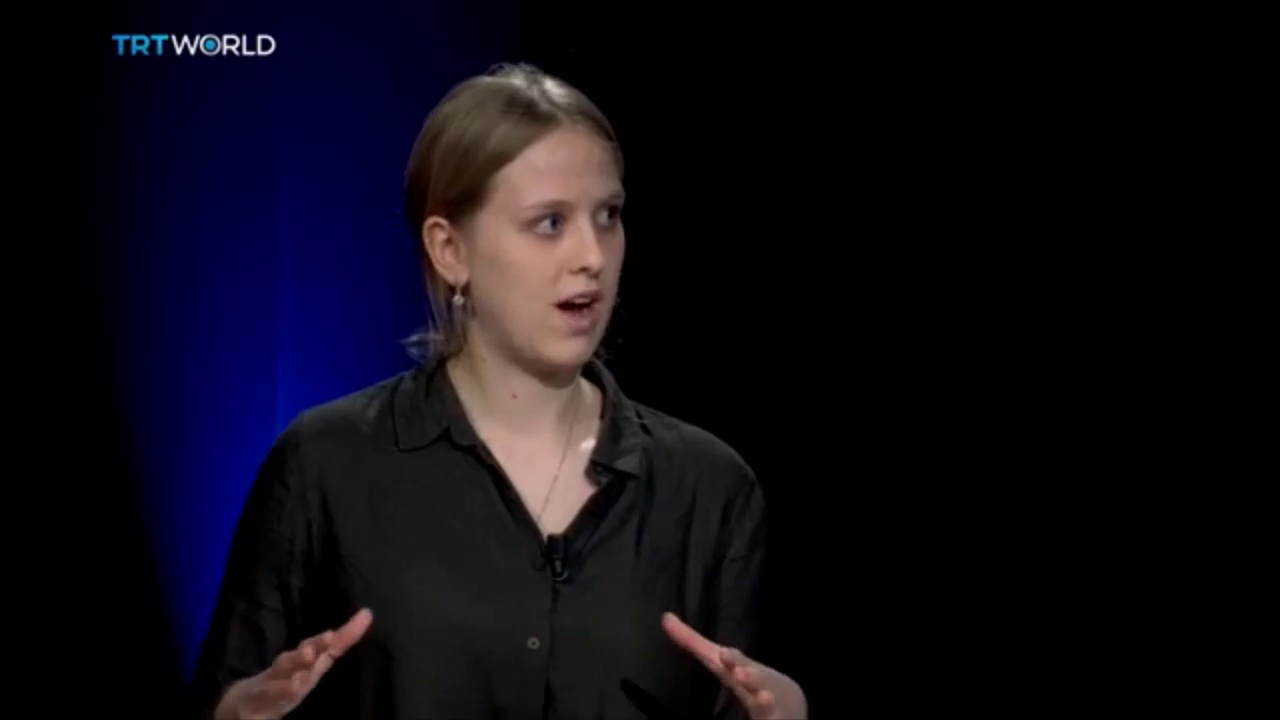
\includegraphics{Figures/play1.png}}{VPlayer.swf}
\end{center}

\texttt{[the] \annotate{direct impact}\textsuperscript{1} will likely result in biodiversity loss that will be very difficult to \annotate{recover from}\textsuperscript{2} but we really don't understand is any of the \annotate{wider impacts}\textsuperscript{3} as well, so outside the \annotate{area of}\textsuperscript{4} mining itself how will this \annotate{affect the ecosystem at large how will this feedback into the oceans}\textsuperscript{5} we think that the deep sea...}

\end{footnotesize}

\begin{footnotesize}
\begin{enumerate}
   \item HAND downward in swift movement, fingers pointed outward
   \item HANDS in cycling motion forward
   \item HANDS expanding outwards
   \item HAND in wide circular movement with palm down
   \item HANDS in cycling movement with palms inwards
\end{enumerate}
\end{footnotesize}

\begin{figure}[H]
\centering
\begin{tabular}{llll}
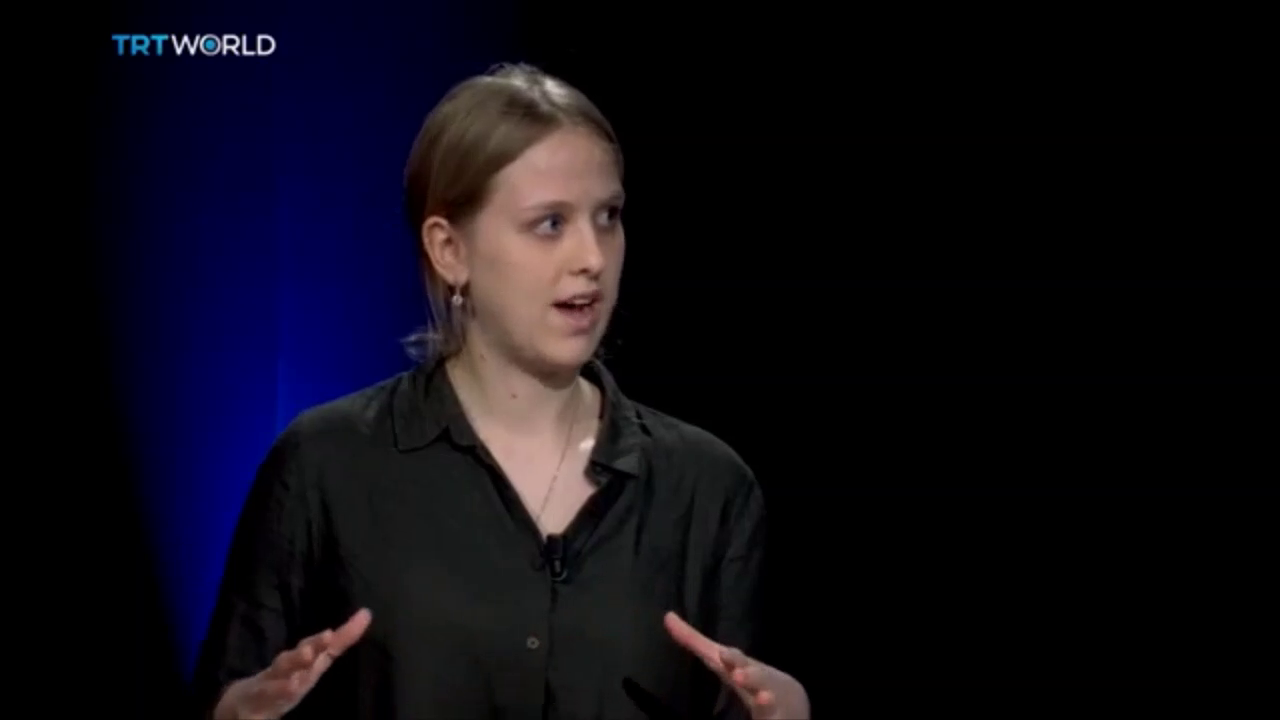
\includegraphics[width=4.2cm]{Figures/mmEco/frame207.png} & 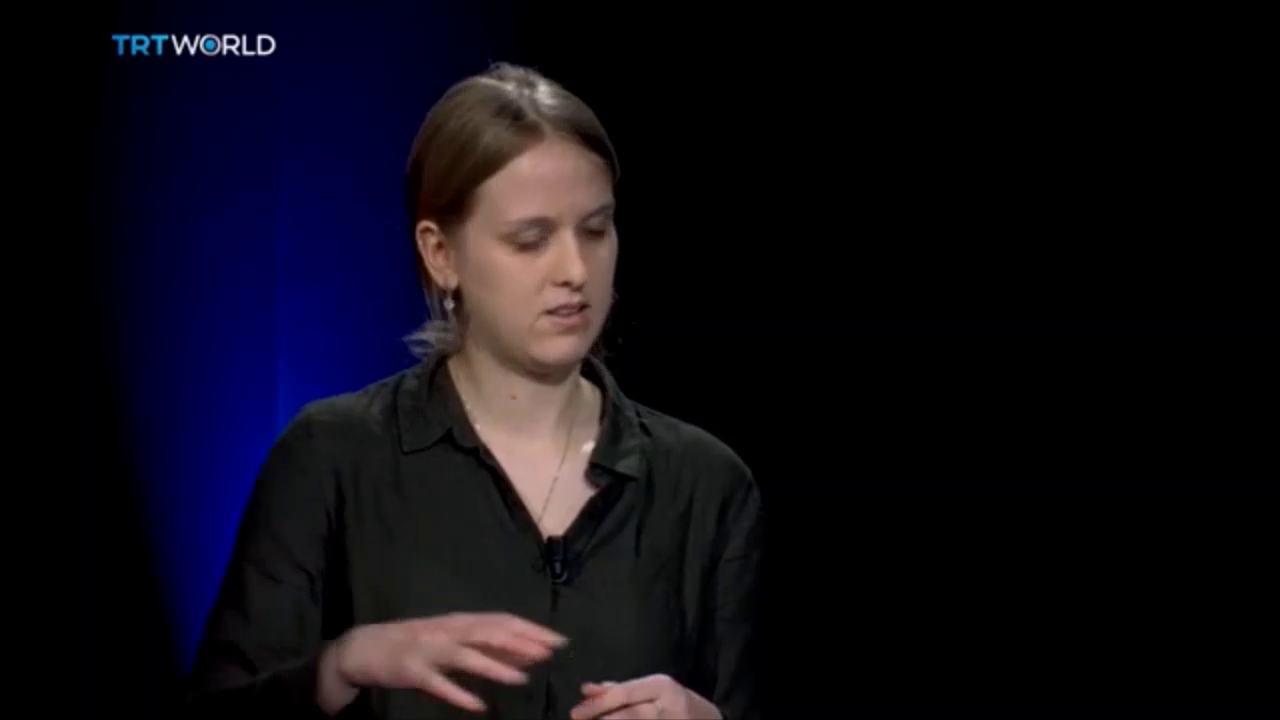
\includegraphics[width=4.2cm]{Figures/mmEco/frame252.png} & 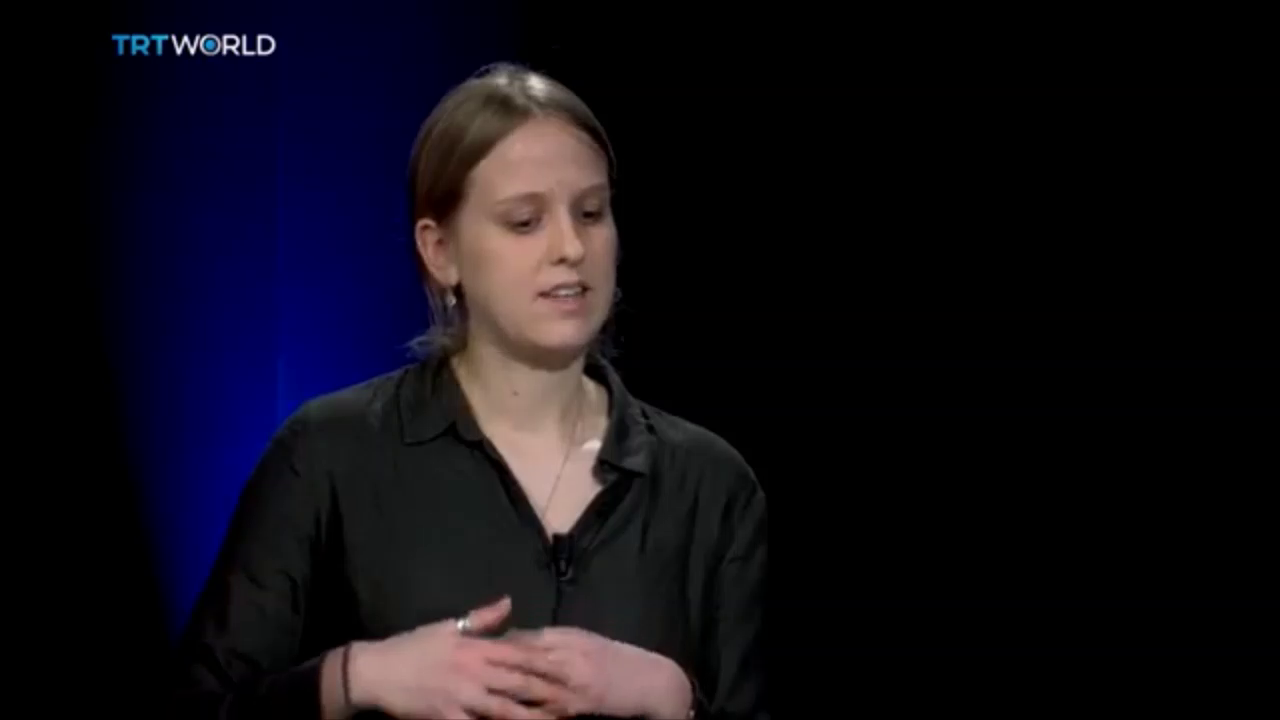
\includegraphics[width=4.2cm]{Figures/mmEco/frame392.png} 

\end{tabular}
\caption{Ecological Level - Example 1}

\begin{footnotesize}
Left: hands open palms down gesture with fingers extended to emphasize direct ecological impacts. Middle, Right: Hands loosened, palms inward/down in a cycling motion to reflect less certain long term ecological processes and feedback mechanisms.


\end{footnotesize}



\label{fig:figure1}
\end{figure}

\subsection{Ecological Level - Example 2}

\begin{footnotesize}
Source: \url{https://www.youtube.com/embed/Sh0_Wf8F4RM?start=857&end=888)}\\
\textit{Embeded videos require Adobe Flash.}
\begin{center}
\includemedia[width=9.60cm,height=5.40cm,activate=pageopen,
passcontext,
transparent,
addresource=Figures/10.mp4,
flashvars={source=Figures/10.mp4}
]{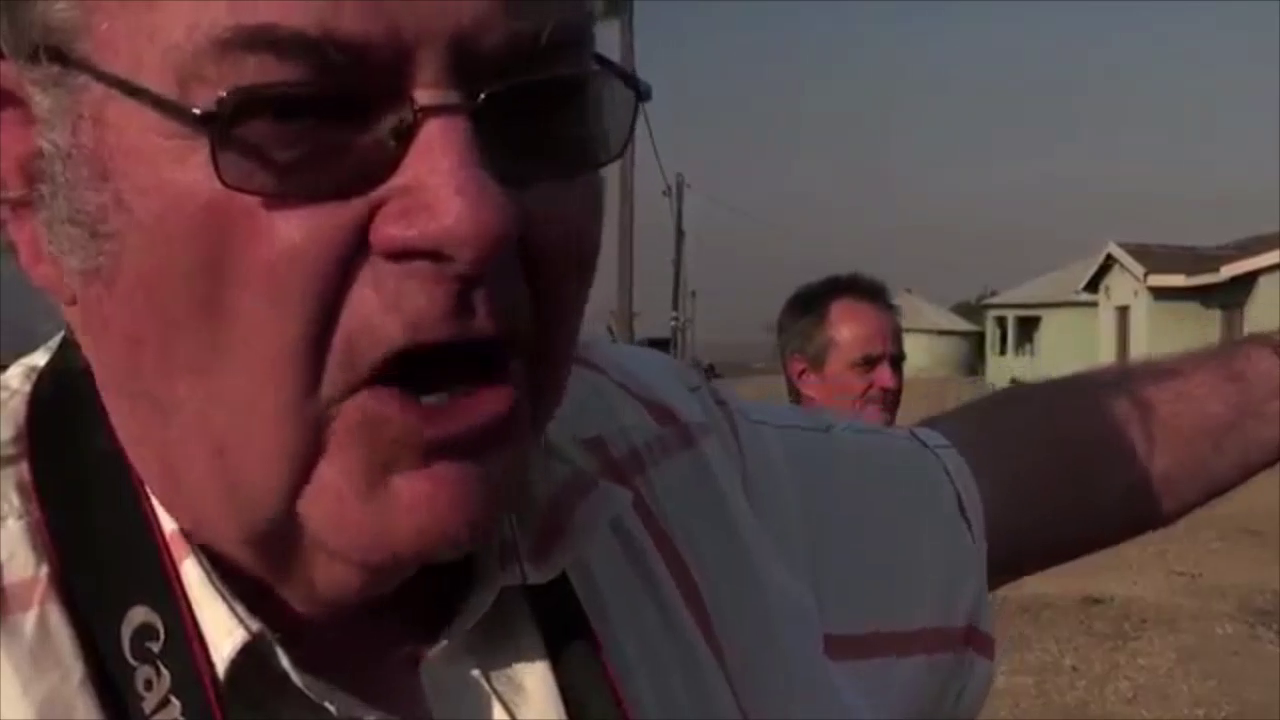
\includegraphics{Figures/play2.png}}{VPlayer.swf}

\end{center}
\end{footnotesize}


\begin{footnotesize}
\texttt{Where our [concern lies is with respect to \annotate{dust}!- because there's no analysis of the dust(.) in terms of the toxic components in that dust]\textsuperscript{1} given the coal mining and the blasting and that sort of thing\degree. Now, you can feel [\annotate{this wind}. <This wind>]\textsuperscript{2} (.) is blowing across us [right into the game reserve]\textsuperscript{3}, so [if] they mine here, this south-easterly wind will carry the dust and the fallout will be in the park, >in the wilderness area<.}   
\end{footnotesize}

\begin{footnotesize}
\begin{enumerate}
   \item Hand in front facing inwards palms open thumbs up
   \item Hands pointing left hand to left
   \item Hand (right) pointing to the right
\end{enumerate}
\end{footnotesize}

\begin{figure}[H]
\centering
\begin{tabular}{llll}

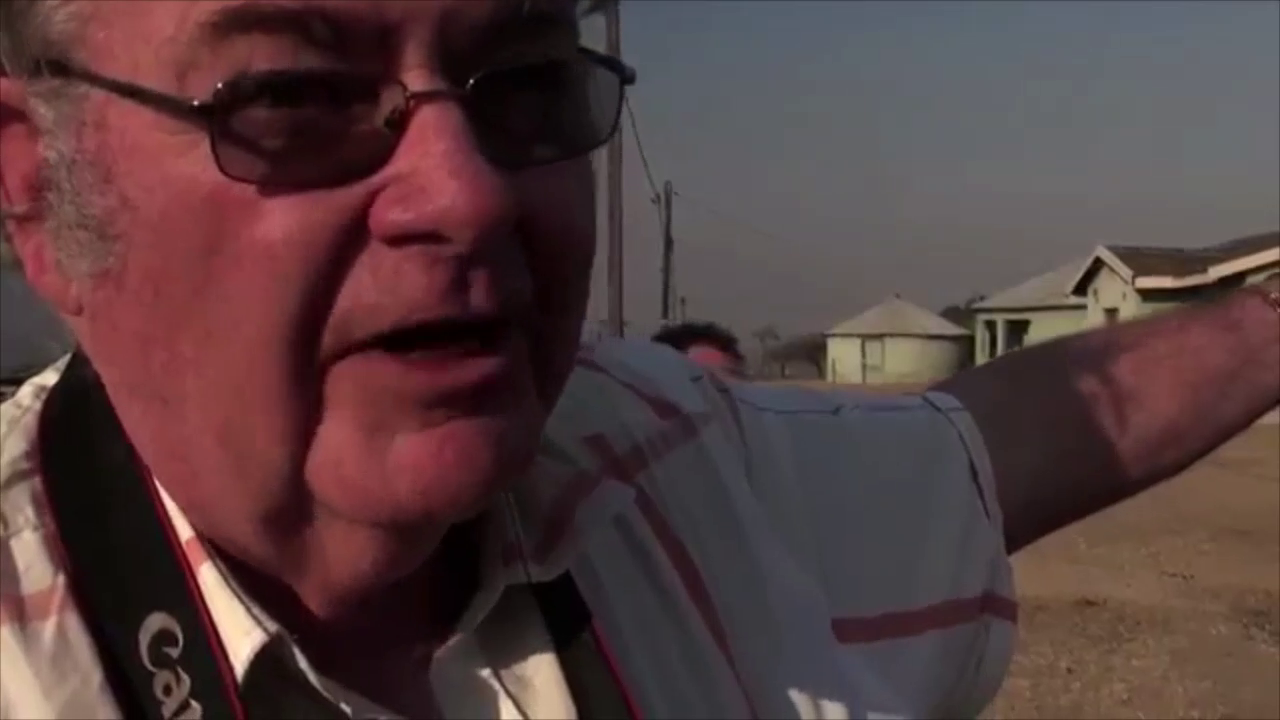
\includegraphics[width=4.2cm]{Figures/mmEco1/frame578.png} & 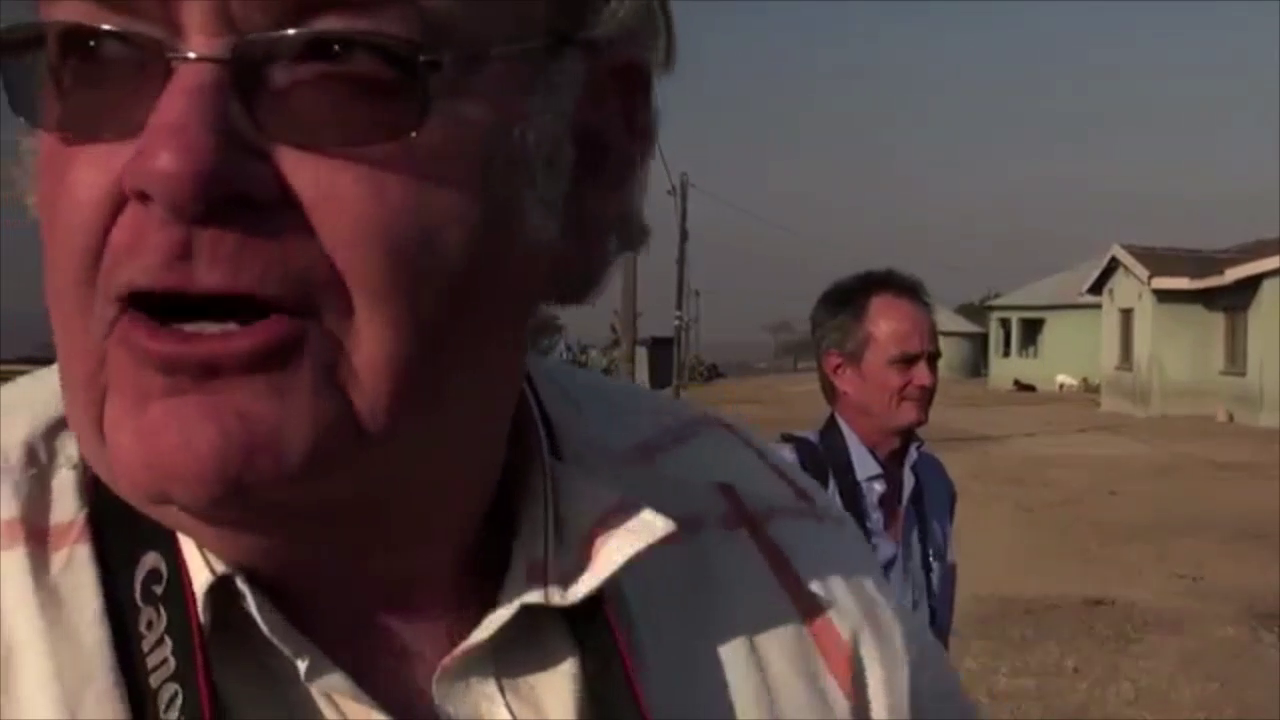
\includegraphics[width=4.2cm]{Figures/mmEco1/frame619.png} & 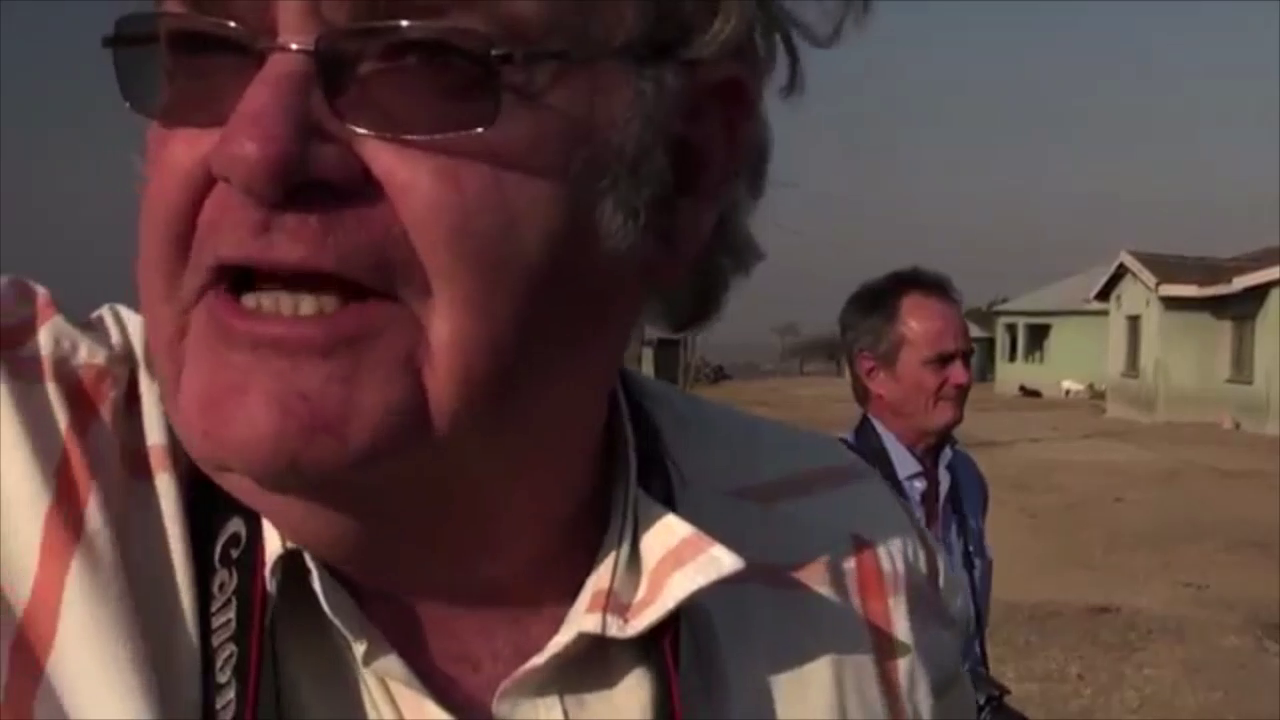
\includegraphics[width=4.2cm]{Figures/mmEco1/frame634.png}  

\end{tabular}
\caption{Ecological Level - Example 2}
\begin{footnotesize}
Hand and arm points to left (Left image) and then to right (Right image) to reflect the physical movement of dust.\\


\end{footnotesize}
\label{fig:figure1}
\end{figure}



\subsection{Ecological Level - Example 3}

\begin{footnotesize}

Source: \url{https://www.youtube.com/embed/UvKe2LYy5pk?start=920&end=945}\\
\textit{Embeded videos require Adobe Flash.}
\begin{center}
\includemedia[width=9.60cm,height=5.40cm,activate=pageopen,
passcontext,
transparent,
addresource=Figures/12.mp4,
flashvars={source=Figures/12.mp4}
]{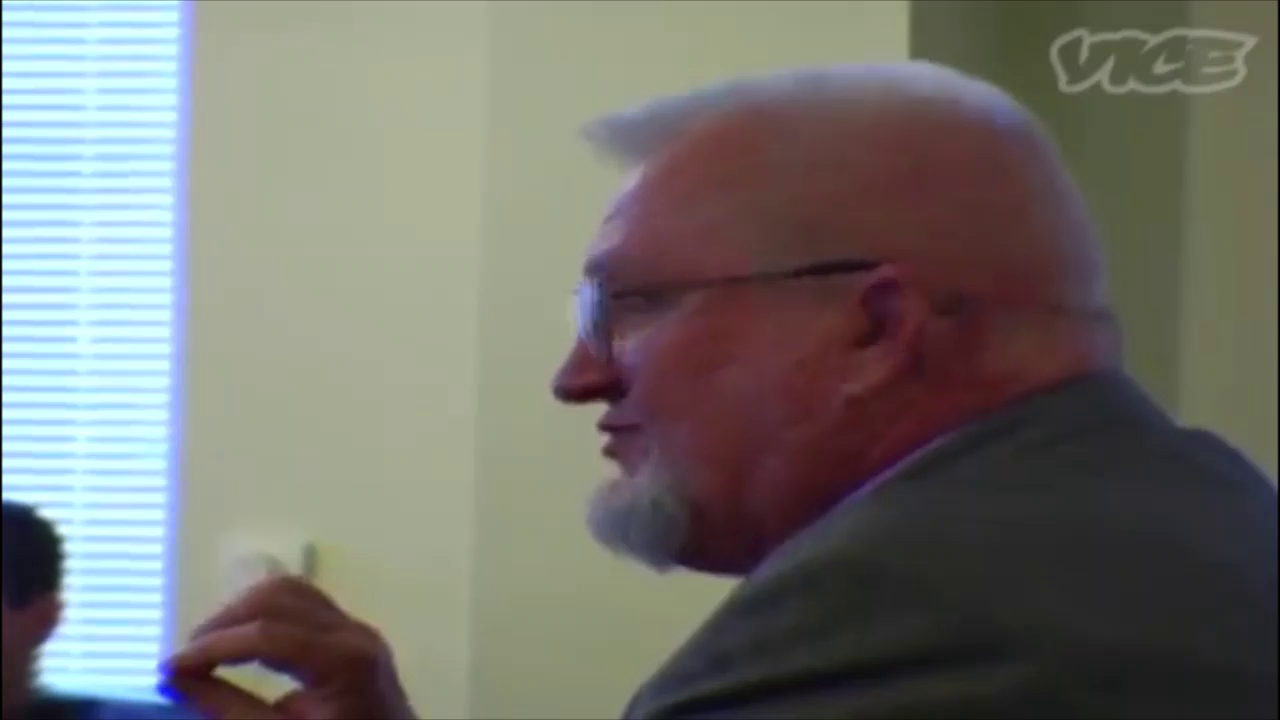
\includegraphics{Figures/play3.png}}{VPlayer.swf}
\end{center}


\begin{footnotesize}
\texttt{People don't understand that <you have to> >[maintain a well just like you do your \annotate{car}]<.\textsuperscript{1} A lot of people just [turn on the spigot,]\textsuperscript{2} and they think [it's going to work for them]\textsuperscript{3} (.) when they have <things like iron hydroxide precipitate> (.) and other metals built up in [their wells (and) every time I go out on a well complaint, I tell people]\textsuperscript{4} you [need to have a friend at the local (.) volunteer fire department come out and flush your well (out)]\textsuperscript{5}....}  
\end{footnotesize}

\begin{footnotesize}
\begin{enumerate}
   \item Index finger and thumb together in precision
   \item Turning of index finger and thumb 
   \item Hand out palm up 
   \item Hand out palm up 
   \item Nodding
\end{enumerate}
\end{footnotesize}

\begin{figure}[H]
\centering
\begin{tabular}{llll}

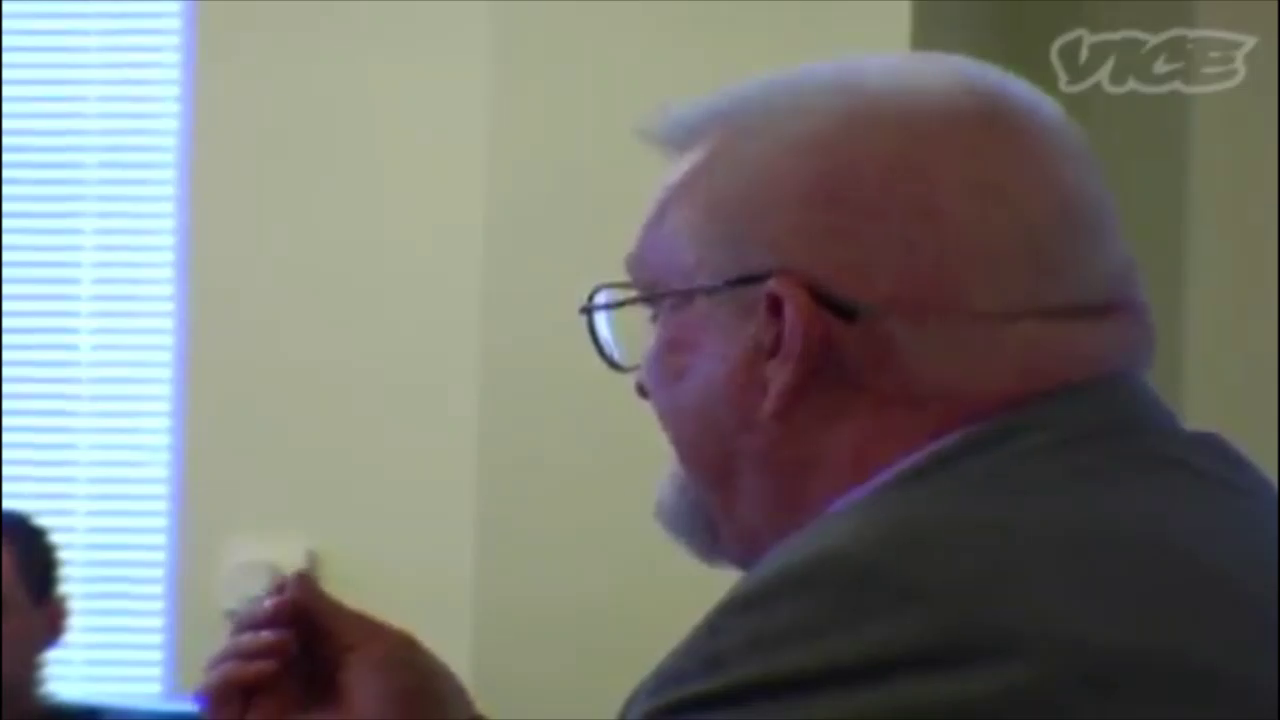
\includegraphics[width=4.2cm]{Figures/mmEco2/frame182.png} & 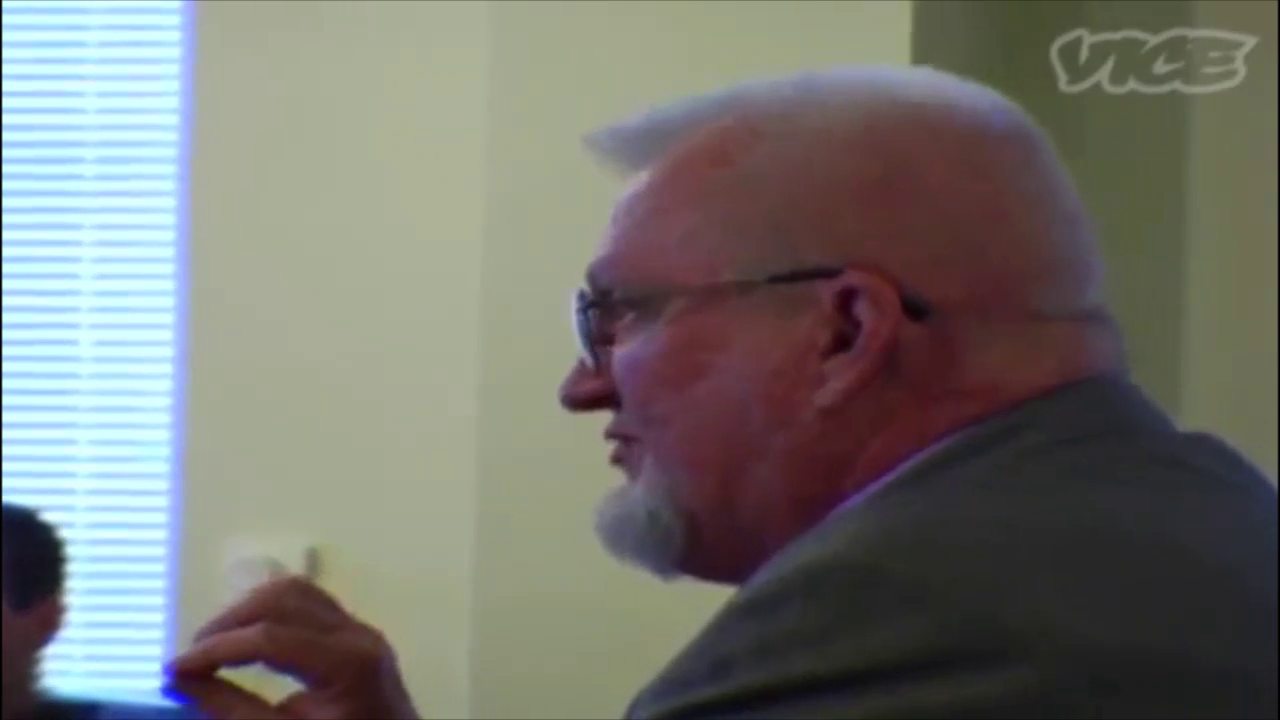
\includegraphics[width=4.2cm]{Figures/mmEco2/frame207.png} & 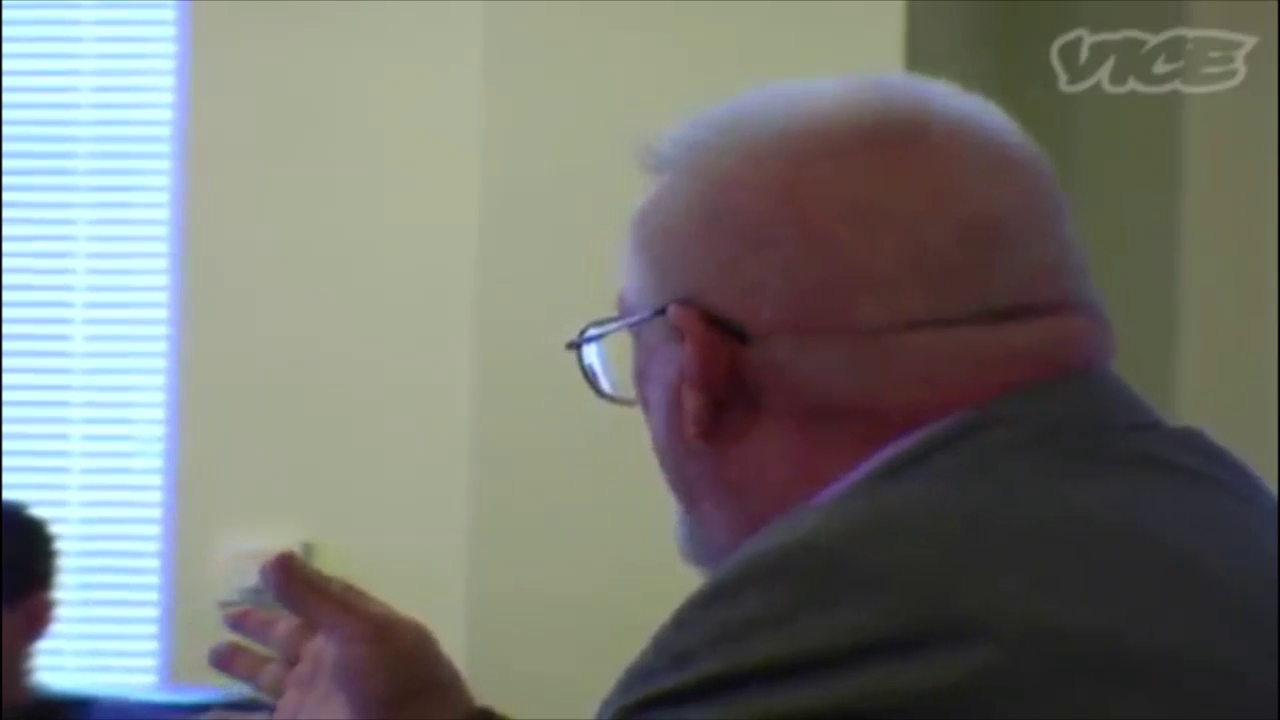
\includegraphics[width=4.2cm]{Figures/mmEco2/frame286.png}  

\end{tabular}
\caption{Ecological Level - Example 3}
\begin{footnotesize}
Left and Middle: the index finger and thumb join to create a precision movement. Right: the open hand palm up gesture functions as a suppliant offer of an idea.\\

\end{footnotesize}
\label{fig:figure1}
\end{figure}

\subsection{Ecological Level - Example 4}

\begin{footnotesize}
Source: \url{https://www.youtube.com/embed/vBhvFWRLiOs?start=821&end=829}\\
\textit{Embeded videos require Adobe Flash.}
\begin{center}
\includemedia[width=9.60cm,height=5.40cm,activate=pageopen,
passcontext,
transparent,
addresource=Figures/18.mp4,
flashvars={source=Figures/18.mp4}
]{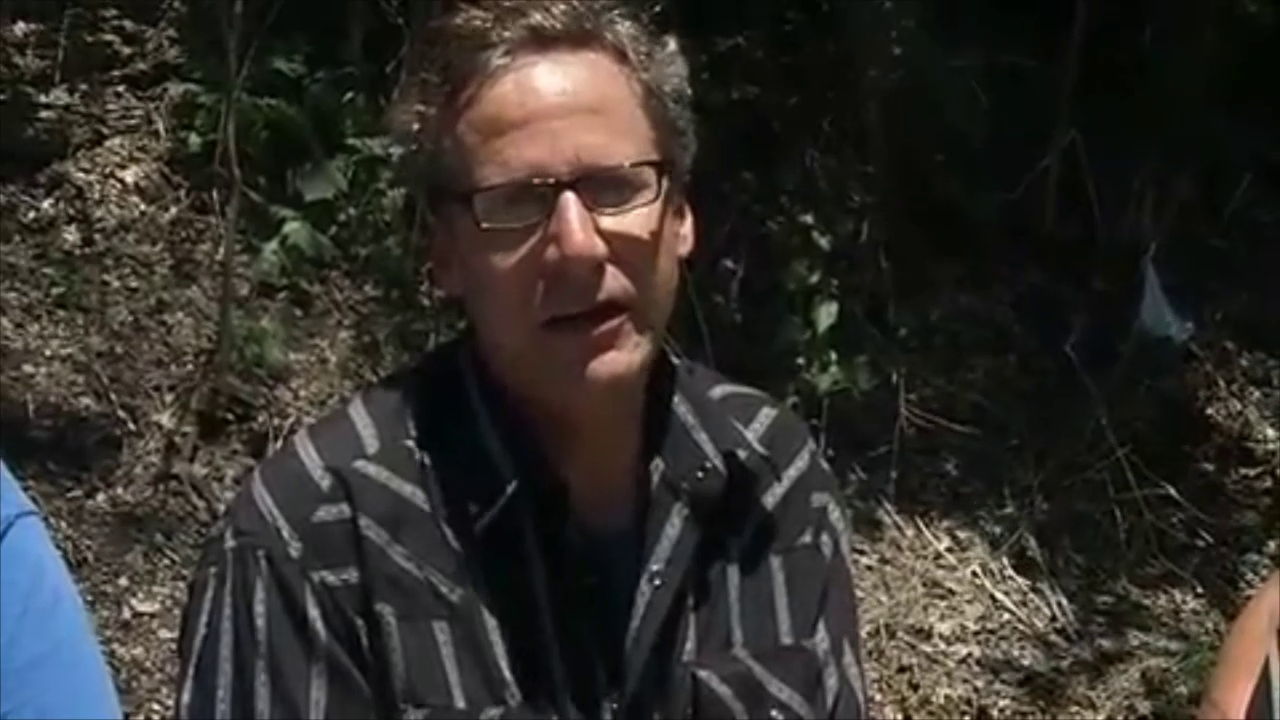
\includegraphics{Figures/play4.png}}{VPlayer.swf}
\end{center}
\end{footnotesize}

\begin{footnotesize}
\texttt{[We've got to build a whole new energy infrastructure for this country, and if we don't we're going to have (.) climate chaos and our kids are going to \annotate{not} thank us for that].\textsuperscript{1}}
\end{footnotesize}

\begin{footnotesize}
\begin{enumerate}
   \item Continuous shaking of HEAD
\end{enumerate}
\end{footnotesize}

\begin{figure}[H]
\centering
\begin{tabular}{llll}

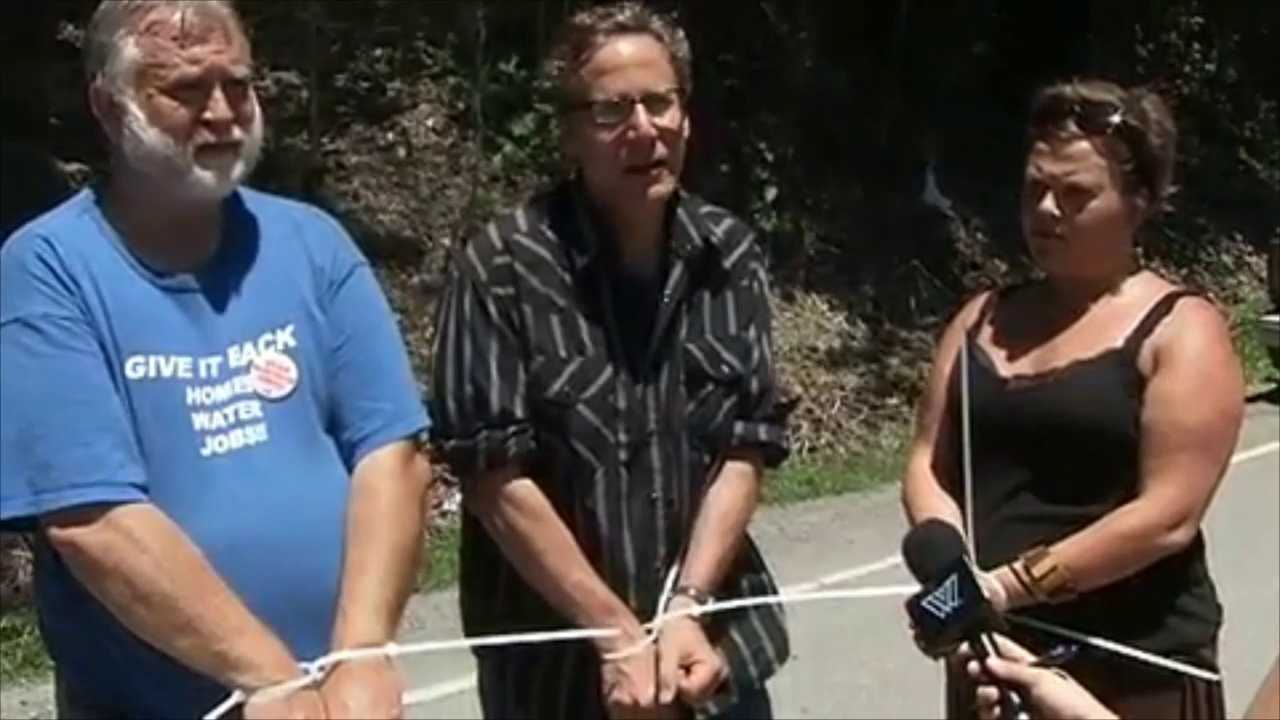
\includegraphics[width=4.2cm]{Figures/mmEco4/frame8.png} & 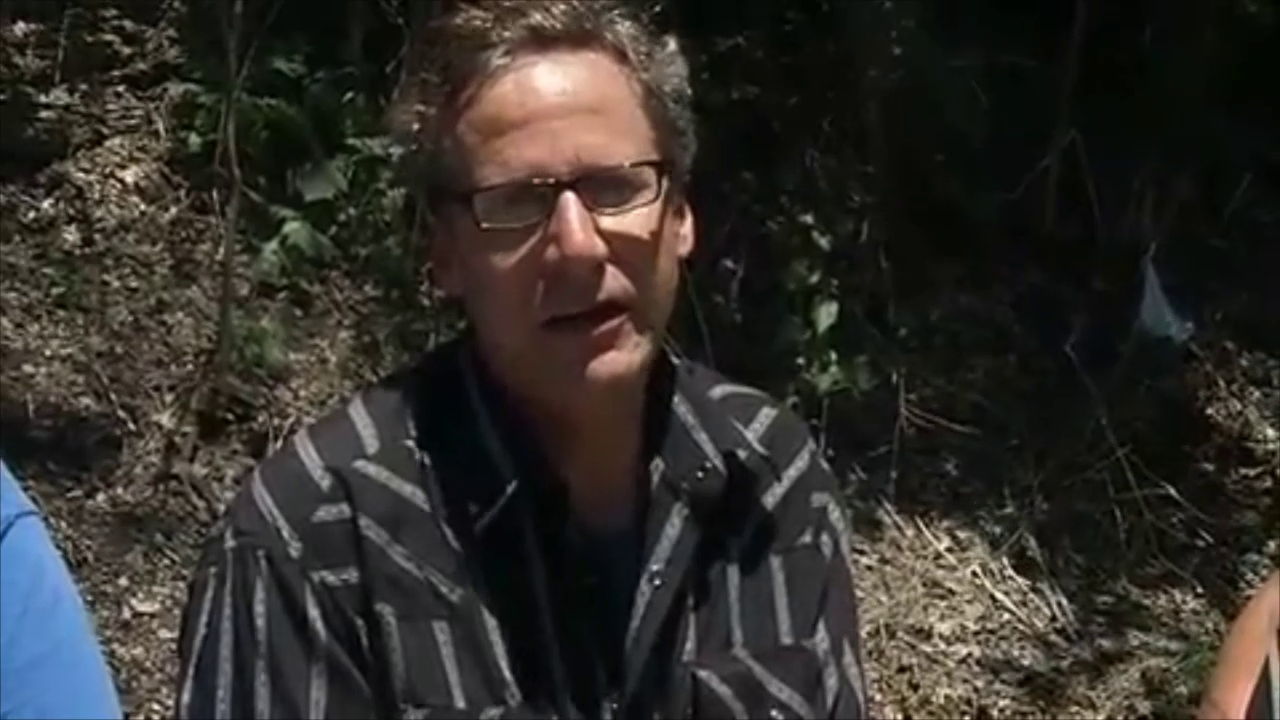
\includegraphics[width=4.2cm]{Figures/mmEco4/frame192.png} & 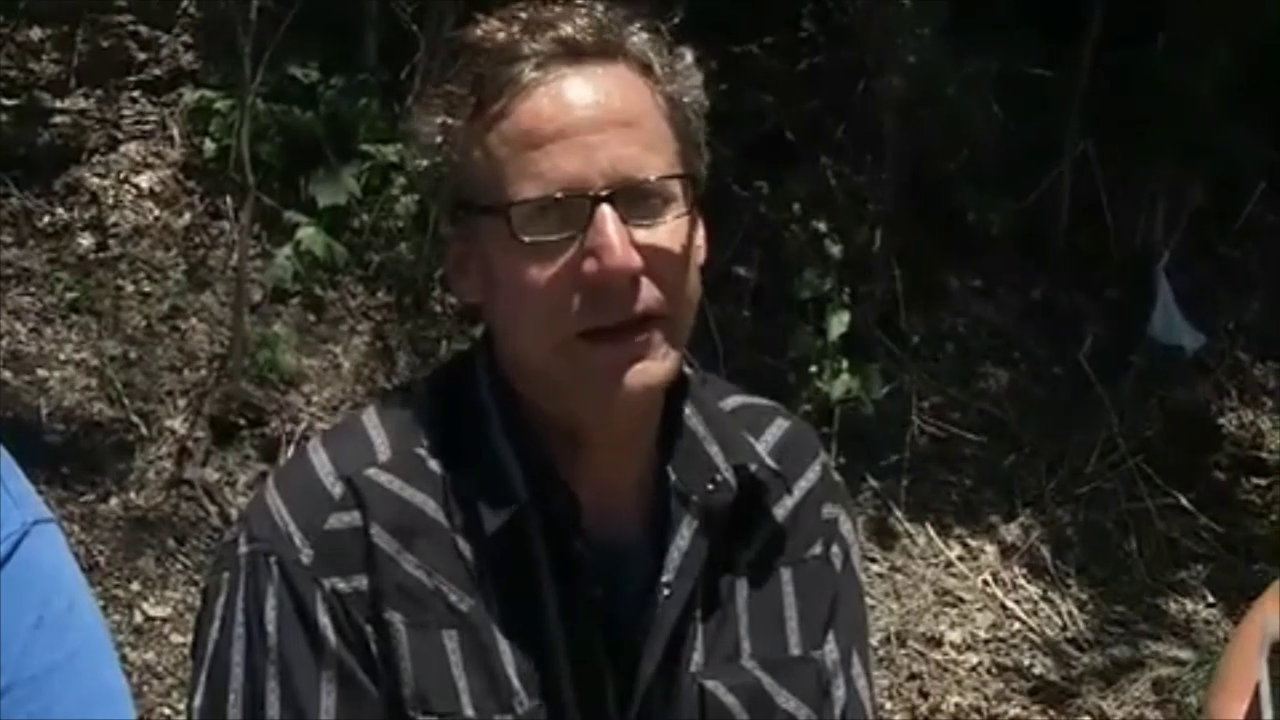
\includegraphics[width=4.2cm]{Figures/mmEco4/frame219.png}  

\end{tabular}
\caption{Ecological Level - Example 4}

\begin{footnotesize}
Left: hands constrained, possible accentuating communicative head movements. Middle, Right: continuous movement (shaking) of head from left to right carrying the meaning of unbelievable.\\

\end{footnotesize}
\label{fig:figure1}
\end{figure}


\section{Cultural-Level}

\subsection{Cultural Level - Example 1}

\begin{footnotesize}
Source: \url{https://www.youtube.com/embed/z6ewpjWYfYo?start=535&end=555}\\
\textit{Embeded videos require Adobe Flash.}
\begin{center}
\includemedia[width=9.60cm,height=5.40cm,activate=pageopen,
passcontext,
transparent,
addresource=Figures/02.mp4,
flashvars={source=Figures/02.mp4}
]{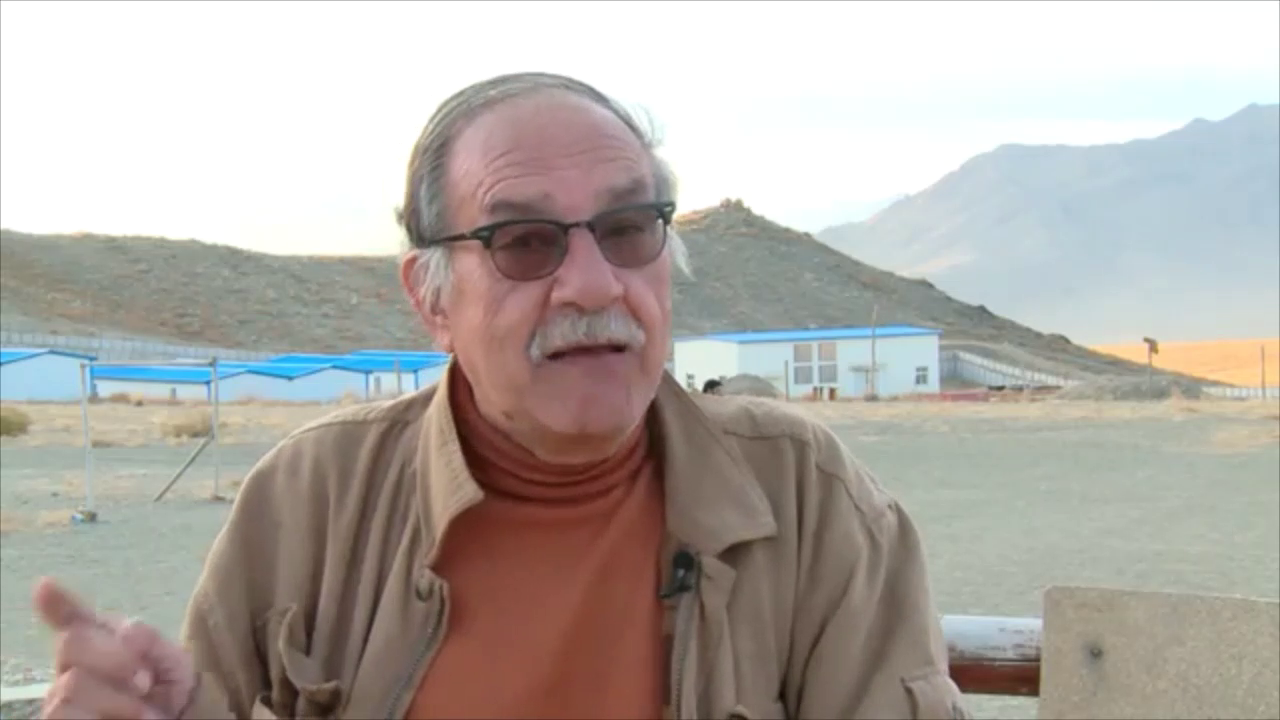
\includegraphics{Figures/play5.png}}{VPlayer.swf}
\end{center}
\end{footnotesize}


\begin{footnotesize}
\texttt{...with [all these wars (over) 30, 40 years]\textsuperscript{1}, (.) what the Afghan has lost we lost [our identity]\textsuperscript{2}!- and [I \annotate{believe}]\textsuperscript{3} to give (them) \annotate{back} that identity is only through [\annotate{culture}]\textsuperscript{4} !- because when it [\annotate{comes}]\textsuperscript{5} to culture, all Afghans are united.}
\end{footnotesize}

\begin{footnotesize}
\begin{enumerate}
   \item Left hand forward palm up; lateral sweep of head and hand
   \item Right hand motion to side; index finger extended; eyebrows raise
   \item Right hand motion to side; index finger extended; head tilts to one side
   \item Right hand motion forward; index finger extended
   \item Right hand motion forward; index finger extended; intonation on ``comes''
\end{enumerate}
\end{footnotesize}

\begin{figure}[H]
\centering
\begin{tabular}{llll}
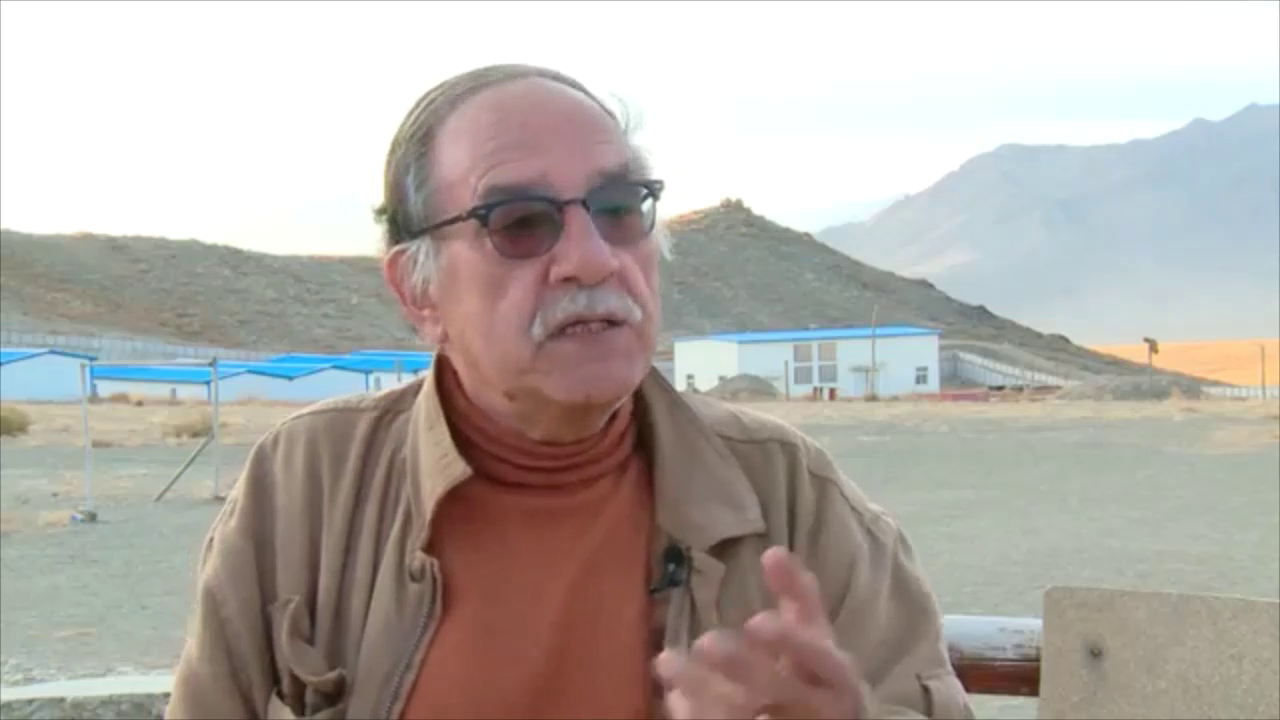
\includegraphics[width=4.2cm]{Figures/mmCult1/frame15.png} & 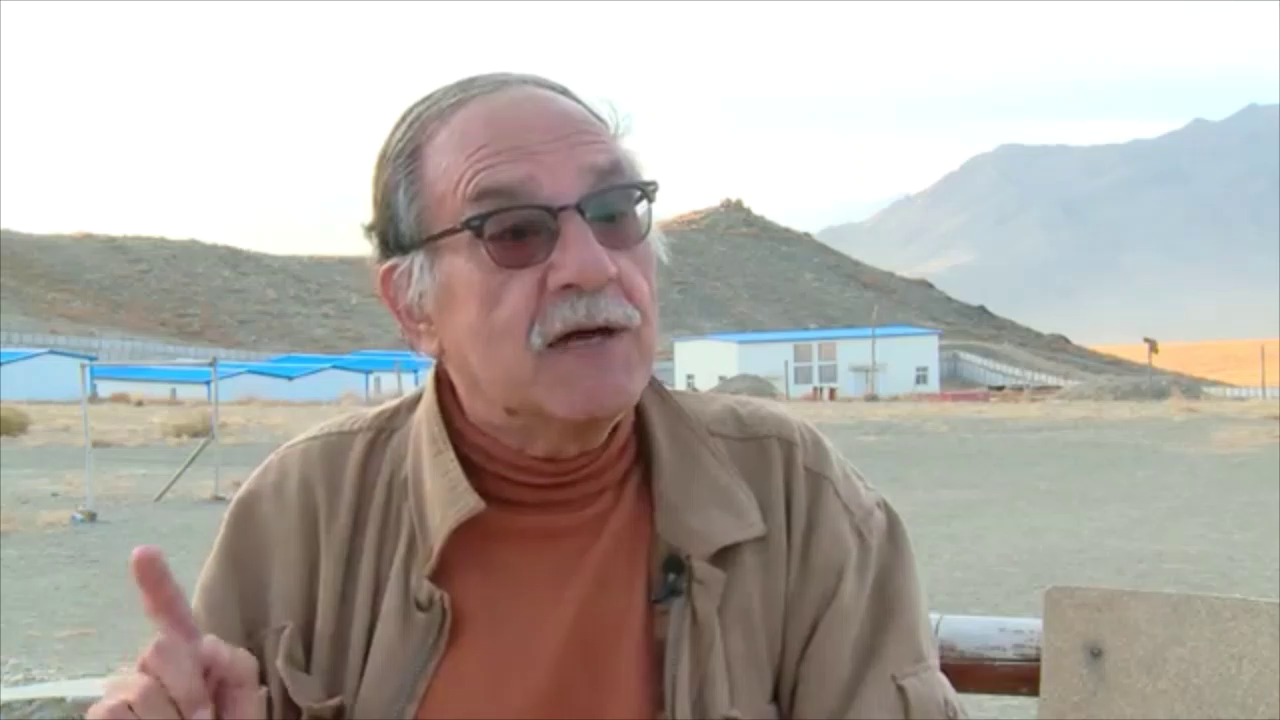
\includegraphics[width=4.2cm]{Figures/mmCult1/frame241.png} & 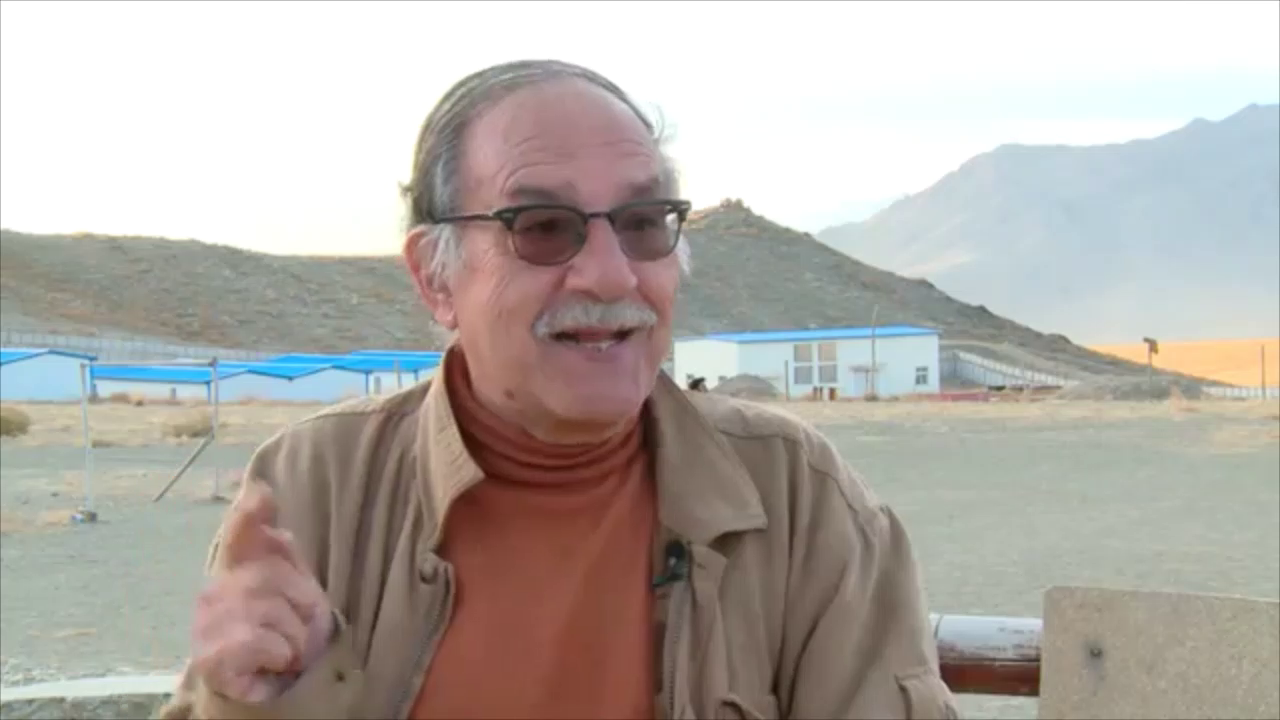
\includegraphics[width=4.2cm]{Figures/mmCult1/frame513.png} 

\end{tabular}
\caption{Cultural level - Example 1}
\begin{footnotesize}

\end{footnotesize}
\label{fig:figure1}
\end{figure}




\subsection{Cultural Level - Example 2}

\begin{footnotesize}
Source: \url{https://www.youtube.com/embed/10FrfEa0Xck?start=33&end=45}\\
\textit{Embeded videos require Adobe Flash.}
\begin{center}
\includemedia[width=9.60cm,height=5.40cm,activate=pageopen,
passcontext,
transparent,
addresource=Figures/03.mp4,
flashvars={source=Figures/03.mp4}
]{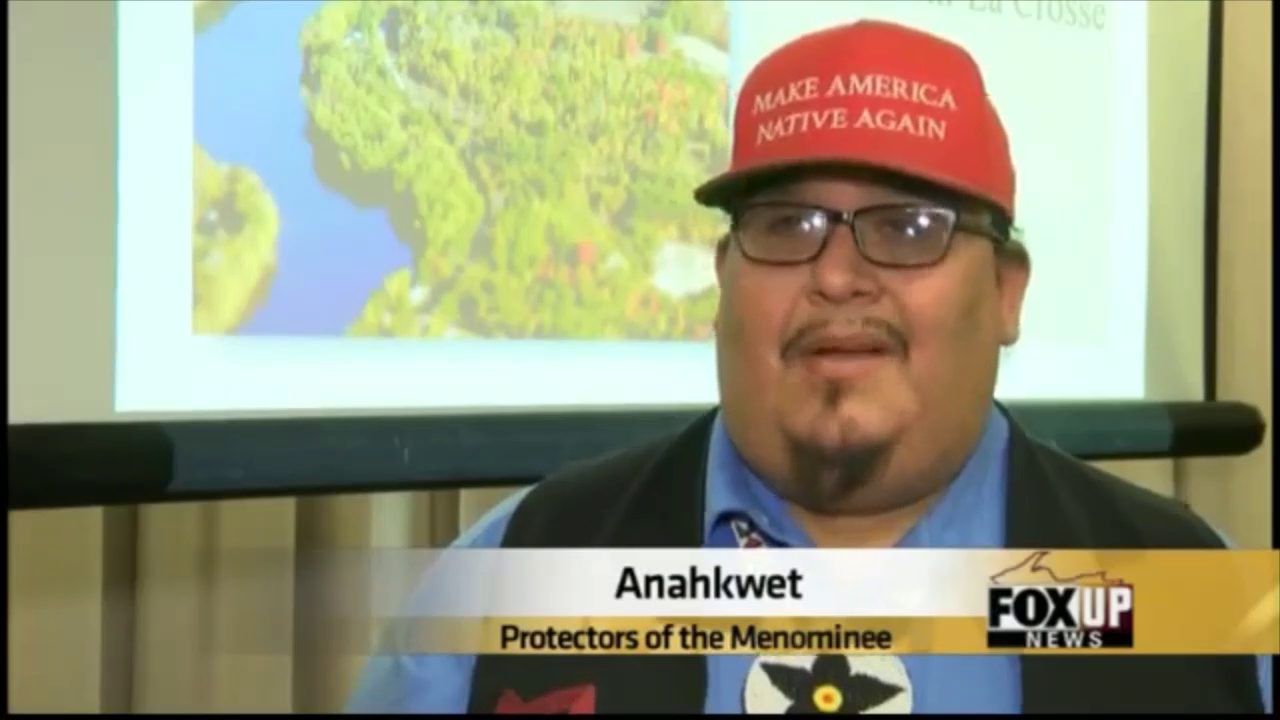
\includegraphics{Figures/mmCult2/frame202.png}}{VPlayer.swf}
\end{center}
\end{footnotesize}




\begin{footnotesize}
\texttt{(It's) [my prehistoric ancestors] (.) that are right within this mining area and [I don't want (.) .hhh hhh you know]\textsuperscript{2} [any \annotate{mine}]\textsuperscript{3} near them, >I don't want any equipment near them.< We have <three known \annotate{burial}> (mound) groups that are there.} 
\end{footnotesize}

\begin{footnotesize}
\begin{enumerate}
   \item Nodding head on beat
   \item Shaking head
   \item Left lip tightened and raised; slight raising of shoulders
\end{enumerate}
\end{footnotesize}

\begin{figure}[H]
\centering
\begin{tabular}{llll}
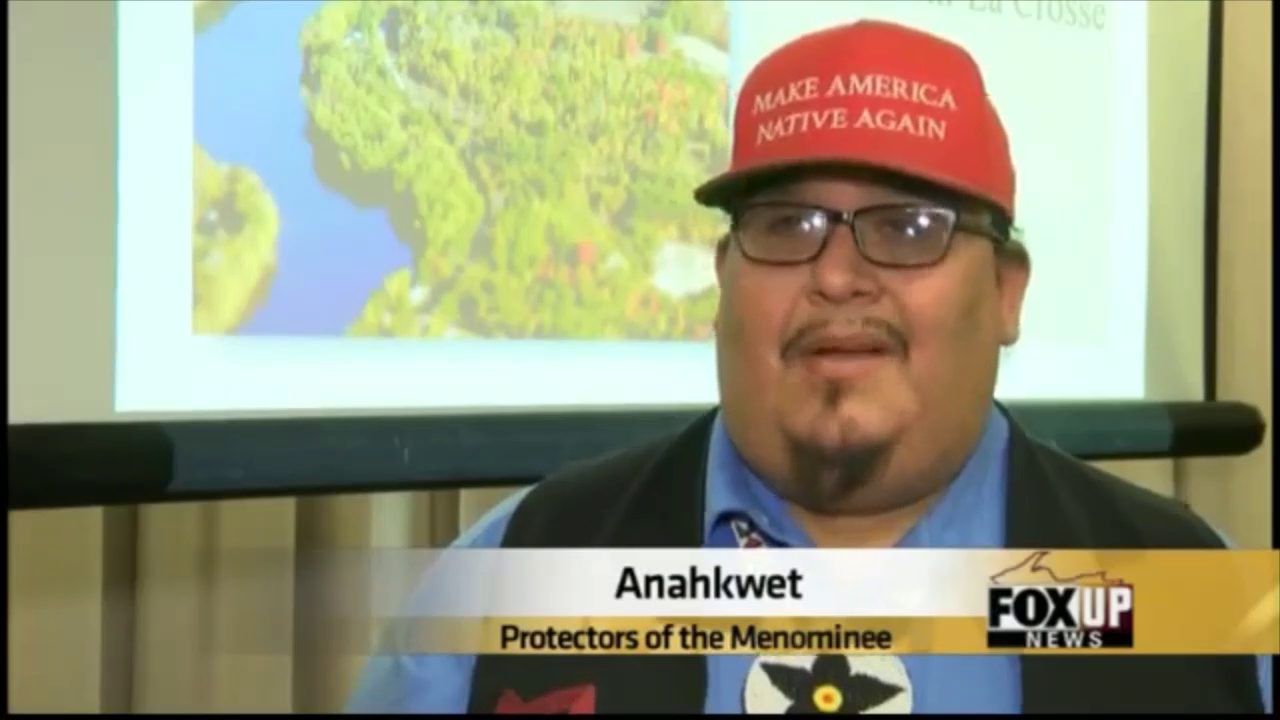
\includegraphics[width=4.2cm]{Figures/mmCult2/frame202.png} & 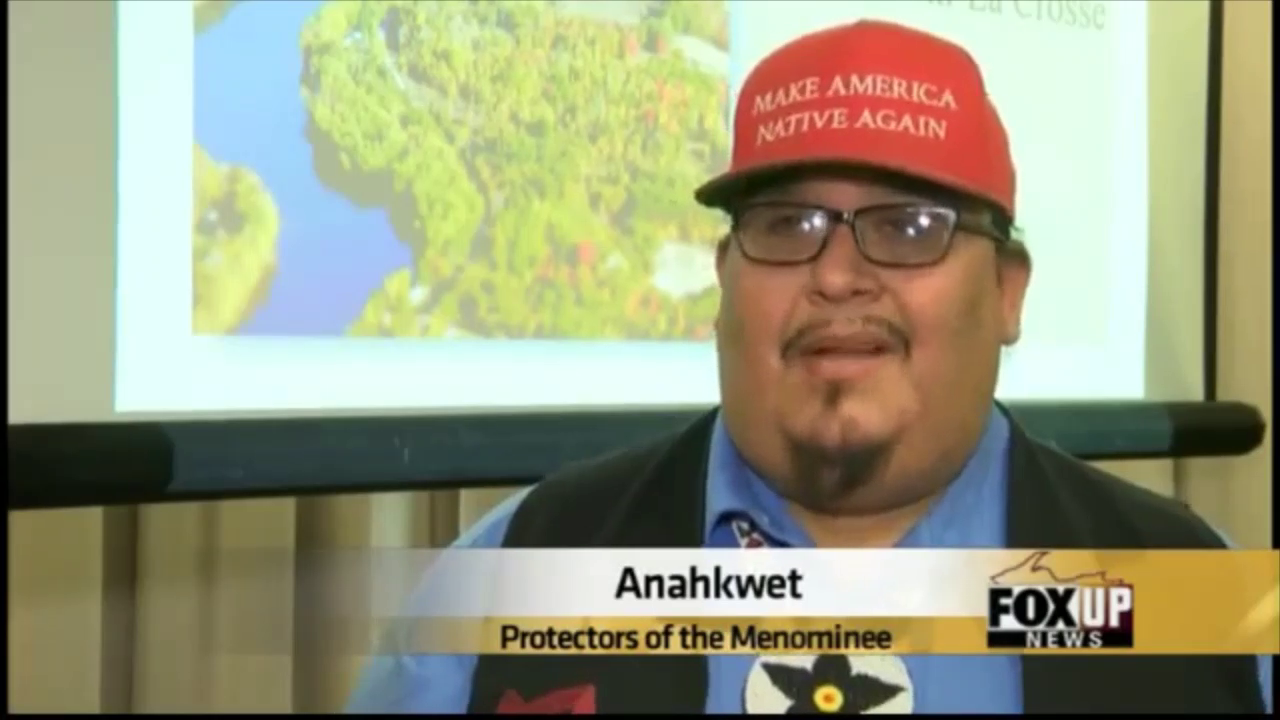
\includegraphics[width=4.2cm]{Figures/mmCult2/frame203.png} & 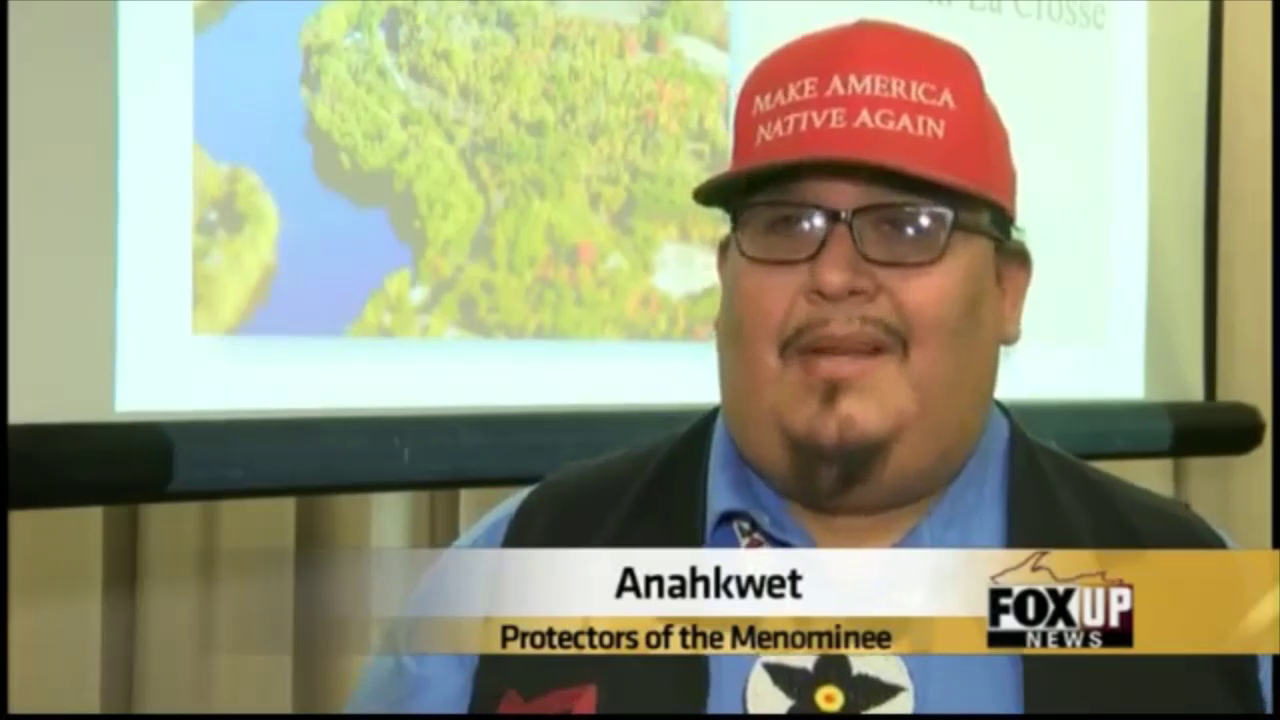
\includegraphics[width=4.2cm]{Figures/mmCult2/frame204.png} 

\end{tabular}
\caption{Cultural level - Example 2}
\begin{footnotesize}

\end{footnotesize}
\label{fig:figure1}
\end{figure}


\subsection{Cultural Level - Example 3}

\begin{footnotesize}
Source: \url{https://www.youtube.com/embed/awnLI4pRnUM?start=42&end=58}\\
\textit{Embeded videos require Adobe Flash.}
\begin{center}
\includemedia[width=9.60cm,height=5.40cm,activate=pageopen,
passcontext,
transparent,
addresource=Figures/04.mp4,
flashvars={source=Figures/04.mp4}
]{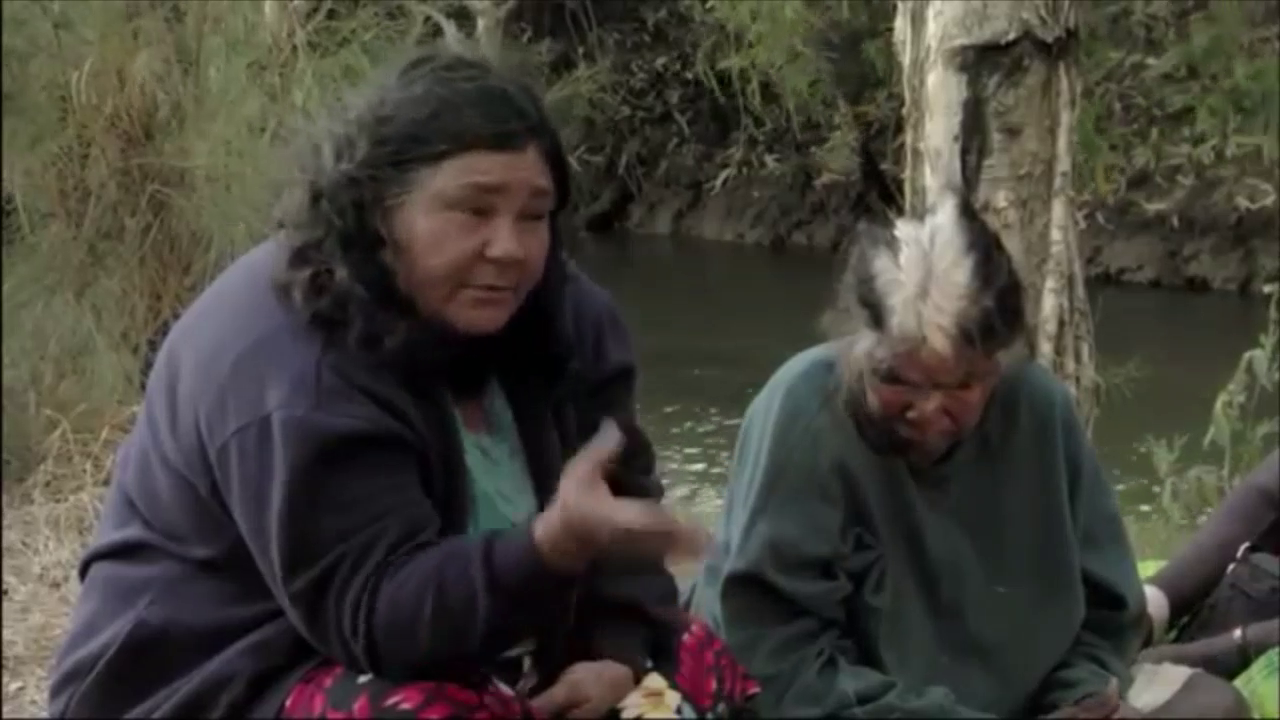
\includegraphics{Figures/mmCult3/frame75.png}}{VPlayer.swf}
\end{center}
\end{footnotesize}



\begin{footnotesize}
\texttt{<[They crushed out sacred site]>. They never [listened to aboriginal people, <elders, female elders>] (.) you know they've been [\annotate{stomped} on]. So it's time for them to \annotate{stand} up and say [hey you're not doing this to me anymore].} 
\end{footnotesize}

\begin{footnotesize}
\begin{enumerate}
   \item Right hand motion forward on beat; palm up; index finger and thumb touching
   \item Right hand motion forward on beat; palm up; fingers and thumb open; high blink rate
   \item Head swipe, left to right with emphasis
   \item Head motion with clenched fist
\end{enumerate}
\end{footnotesize}

\begin{figure}[H]
\centering
\begin{tabular}{llll}

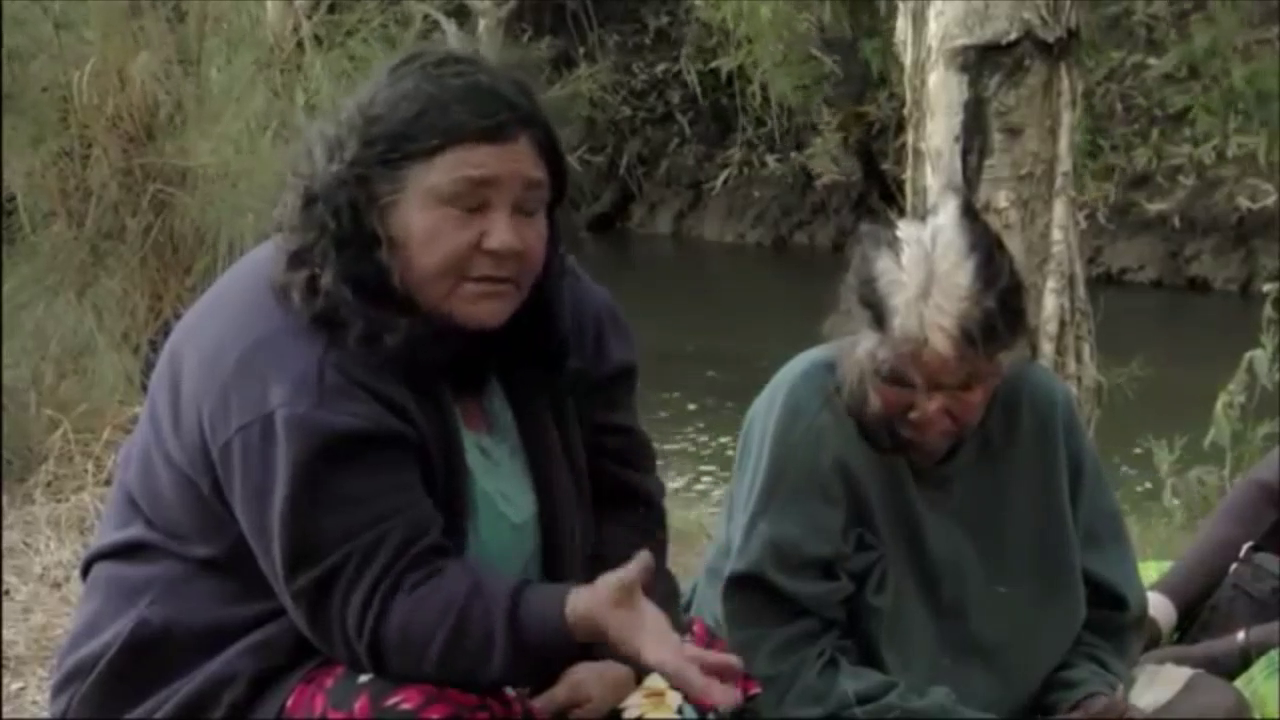
\includegraphics[width=4.2cm]{Figures/mmCult3/frame85.png} & 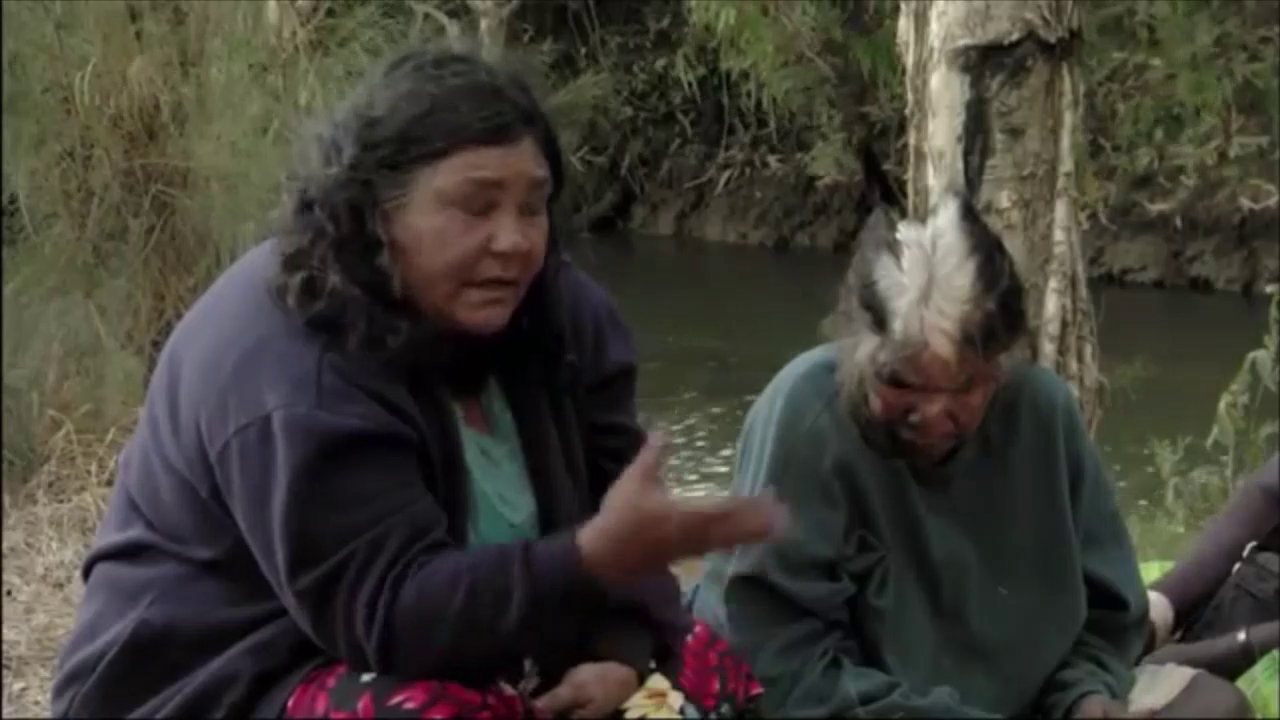
\includegraphics[width=4.2cm]{Figures/mmCult3/frame128.png} & 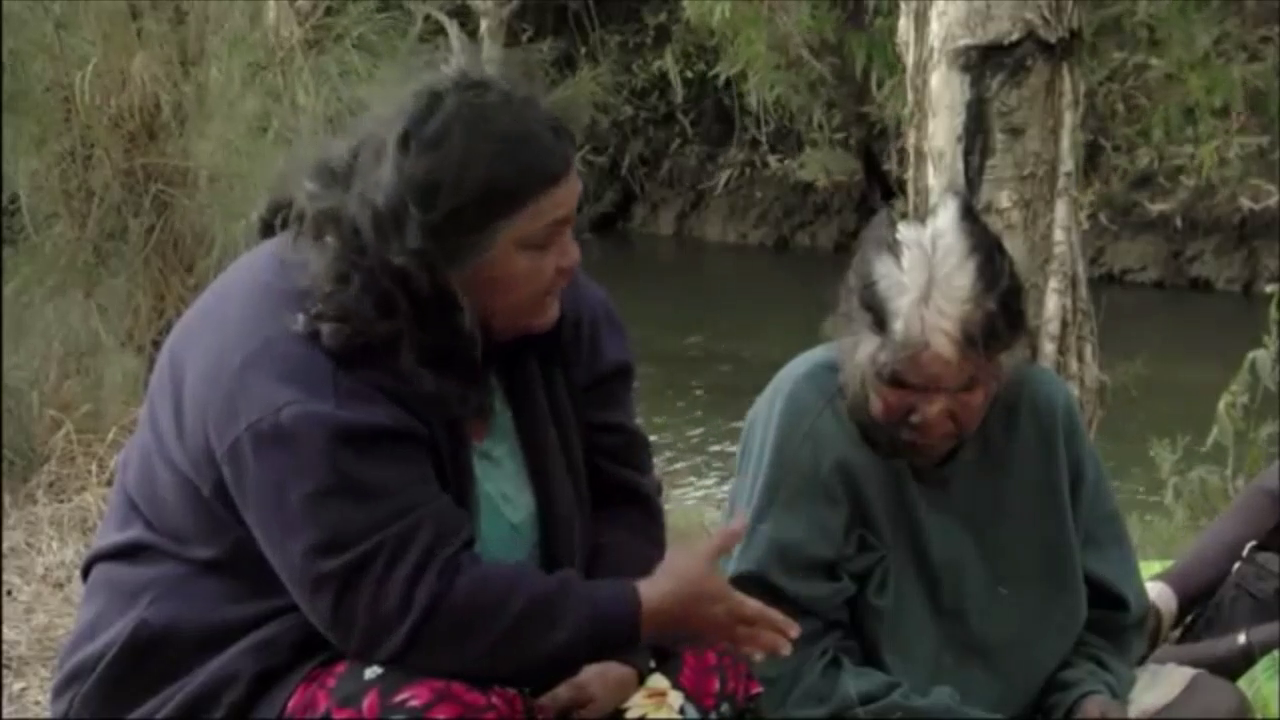
\includegraphics[width=4.2cm]{Figures/mmCult3/frame141.png}  

\end{tabular}
\caption{Cultural Level - Example 3}
\begin{footnotesize}

\end{footnotesize}
\label{fig:figure1}
\end{figure}



\subsection{Cultural Level - Example 4}

\begin{footnotesize}
Source: \url{https://www.youtube.com/embed/UvKe2LYy5pk?start=1198&end=1220}\\\\
\textit{Embeded videos require Adobe Flash.}
\begin{center}
\includemedia[width=9.60cm,height=5.40cm,activate=pageopen,
passcontext,
transparent,
addresource=Figures/14.mp4,
flashvars={source=Figures/14.mp4}
]{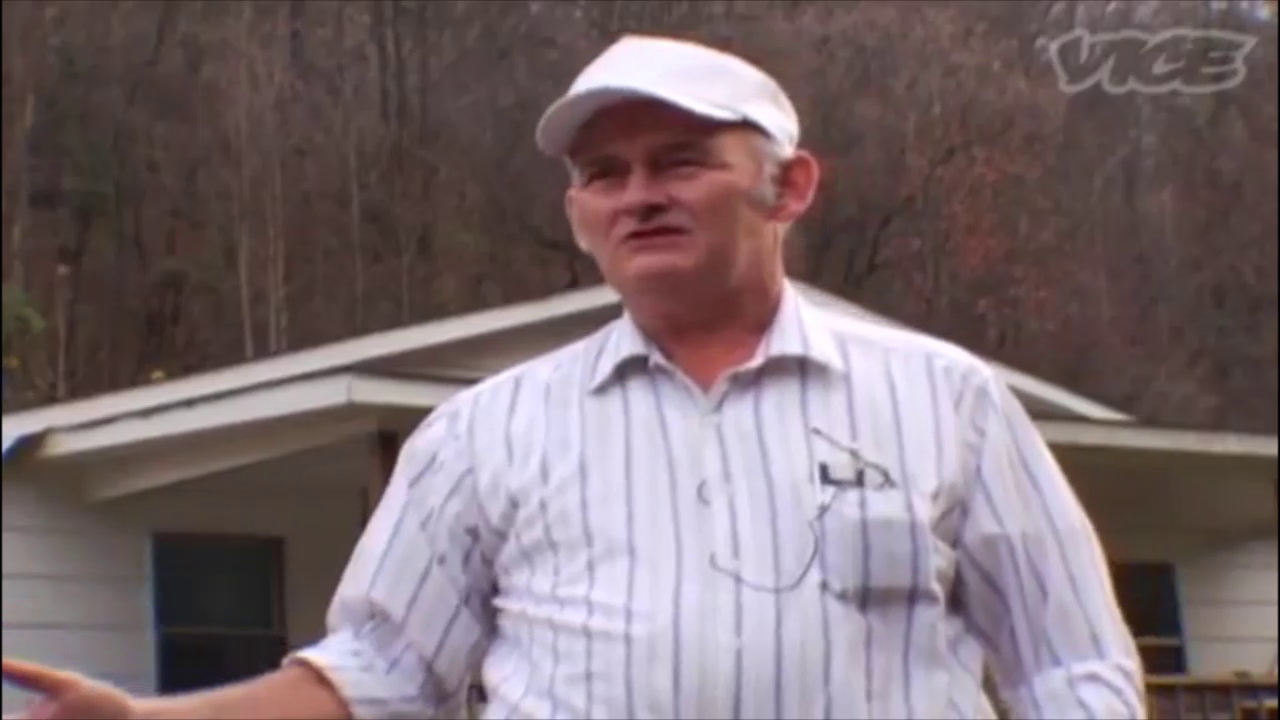
\includegraphics{Figures/mmCult4/frame218.png}}{VPlayer.swf}
\end{center}
\end{footnotesize}


\textbf{\underline{Cultural Level - Example 4}}

\begin{footnotesize}
\texttt{You \annotate{pray} before you go to bed... and >you just ask God to protect (you and) your family, that's all you \annotate{can} do,< because (.) [\annotate{man} has done the damage to the earth (.) and man]\textsuperscript{1} (.) [I don't see how <man can correct what's been done>]\textsuperscript{2}. [\annotate{God} can handle this (.) and he will. When the right time comes]\textsuperscript{3}, he will do what needs to be done.}
\end{footnotesize}

\begin{footnotesize}
\begin{enumerate}
   \item Right hand motions forward; palm up
   \item Right hand motions forward, fingers and thumbs curled inward; head shaking
   \item Rand waves outwards, stops at thigh; gaze upwards to sky; nodding 
\end{enumerate}
\end{footnotesize}

\begin{figure}[H]
\centering
\begin{tabular}{llll}

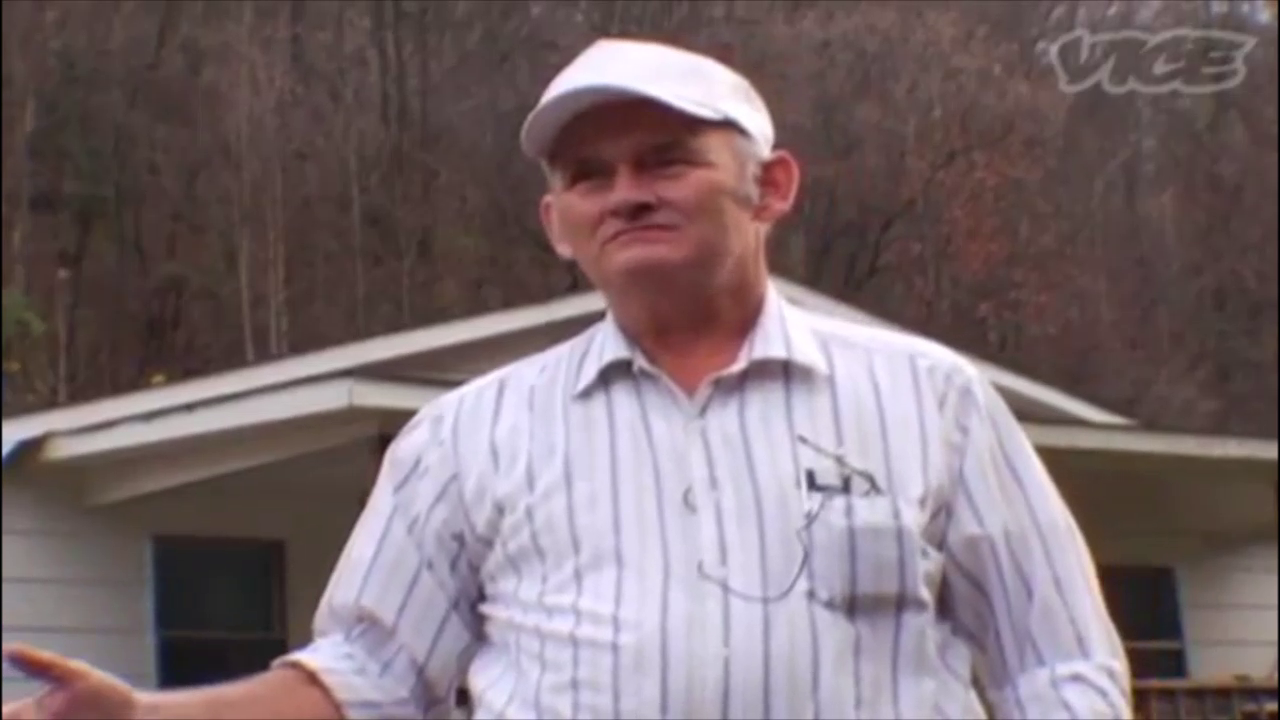
\includegraphics[width=4.2cm]{Figures/mmCult4/frame237.png} & 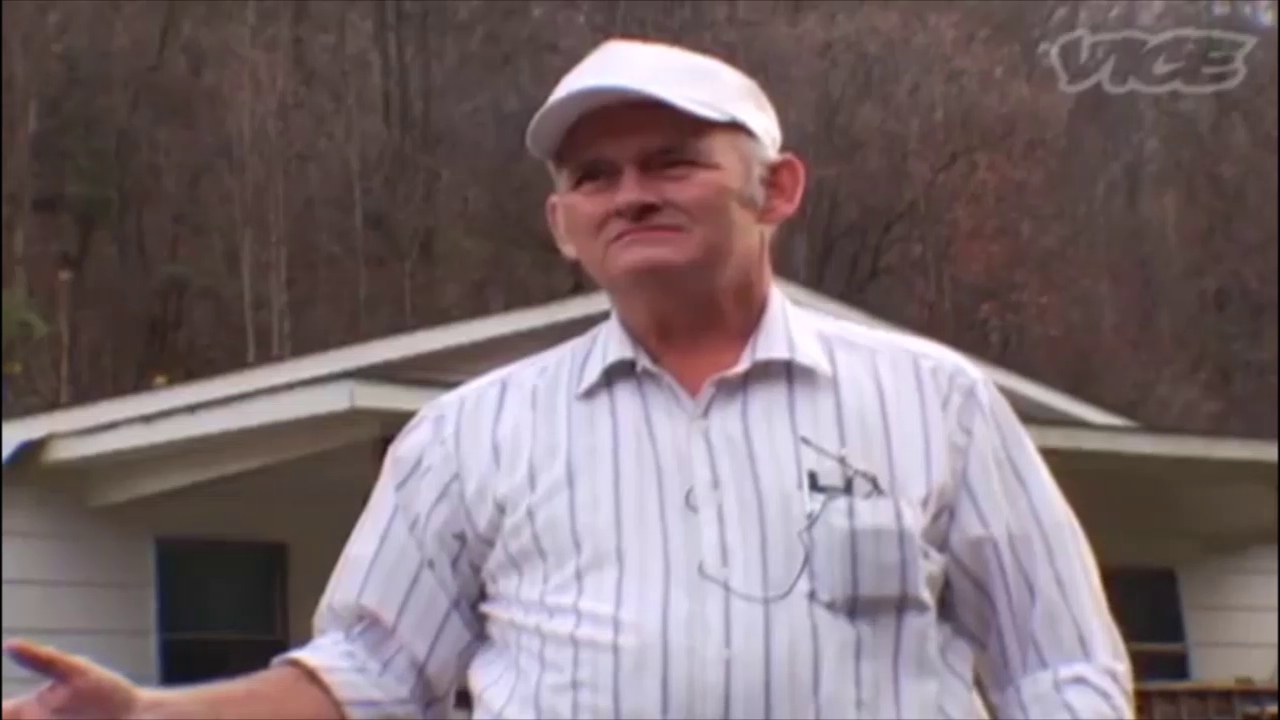
\includegraphics[width=4.2cm]{Figures/mmCult4/frame245.png} & 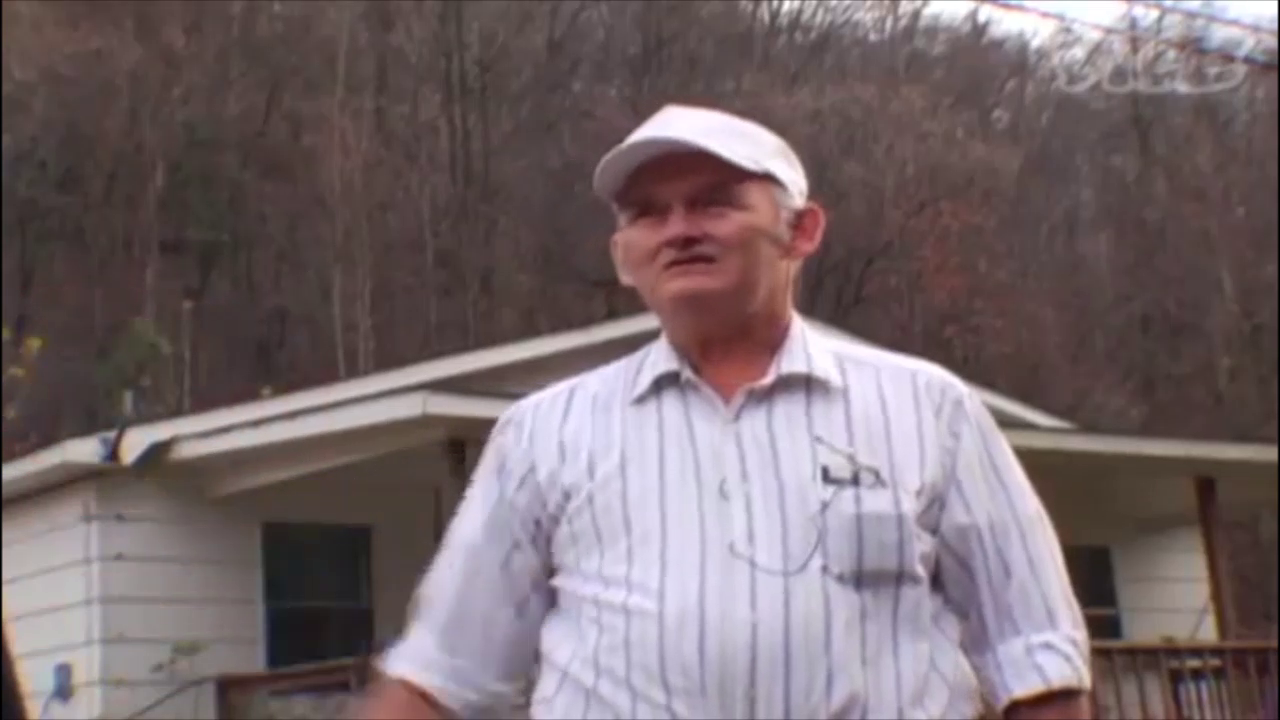
\includegraphics[width=4.2cm]{Figures/mmCult4/frame437.png}  

\end{tabular}
\caption{Cultural level - Example 4}
\begin{footnotesize}

\end{footnotesize}
\label{fig:figure1}
\end{figure}



\subsection{Cultural Level - Example 5}

\begin{footnotesize}
Source: \url{https://www.youtube.com/embed/vBhvFWRLiOs?start=467&end=476}\\
\textit{Embeded videos require Adobe Flash.}
\begin{center}
\includemedia[width=9.60cm,height=5.40cm,activate=pageopen,
passcontext,
transparent,
addresource=Figures/17.mp4,
flashvars={source=Figures/17.mp4}
]{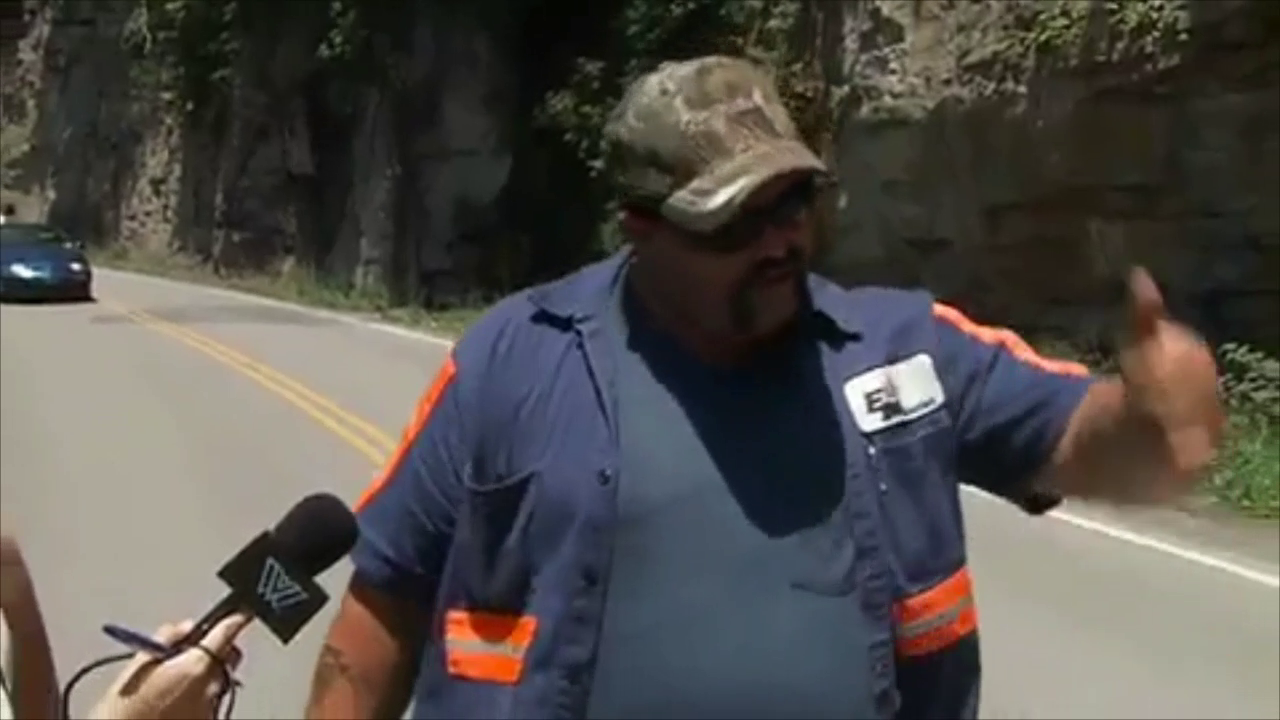
\includegraphics{Figures/mmCult5/frame103.png}}{VPlayer.swf}
\end{center}
\end{footnotesize}

\begin{footnotesize}
\texttt{If [they're for us]\textsuperscript{1}, that's good. If they're [against us, get out]\textsuperscript{2} of the state.}
\end{footnotesize}

\begin{footnotesize}
\begin{enumerate}
   \item Hand motion down towards ground, index finger extended
   \item Thumb up; hand motion back over left shoulder
\end{enumerate}
\end{footnotesize}

\begin{figure}[H]
\centering
\begin{tabular}{llll}

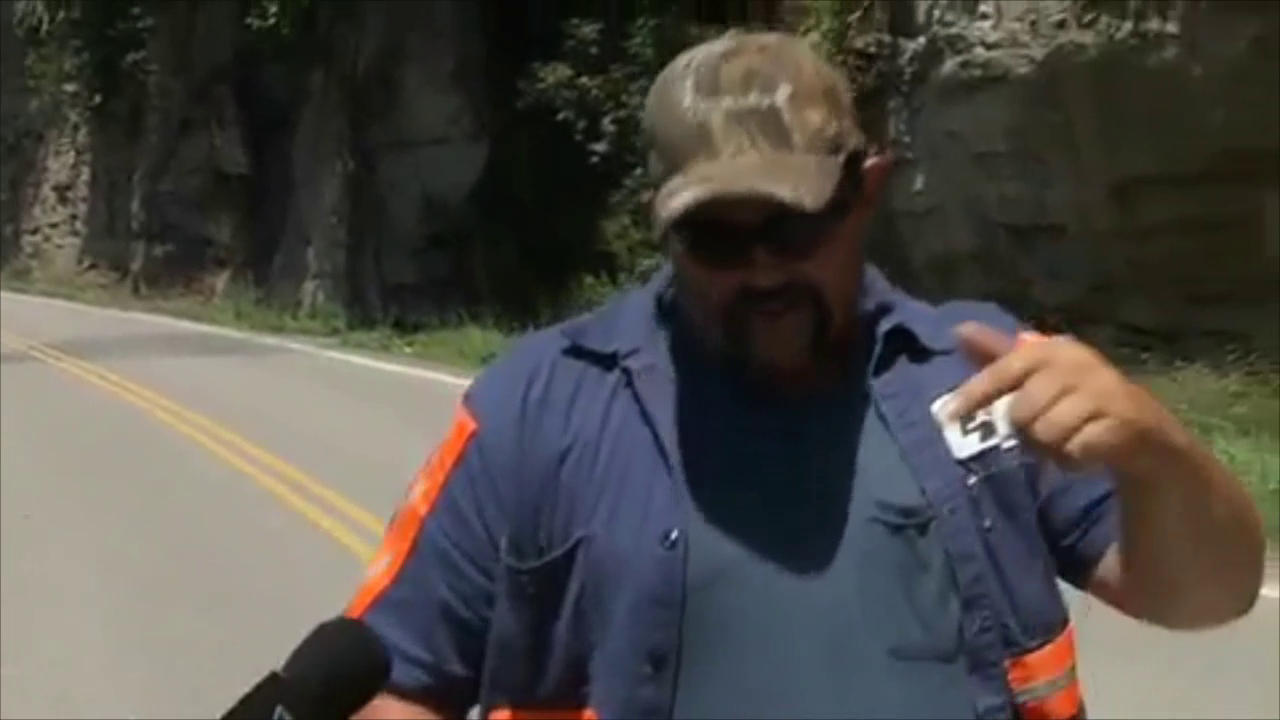
\includegraphics[width=4.2cm]{Figures/mmCult5/frame19.png} & 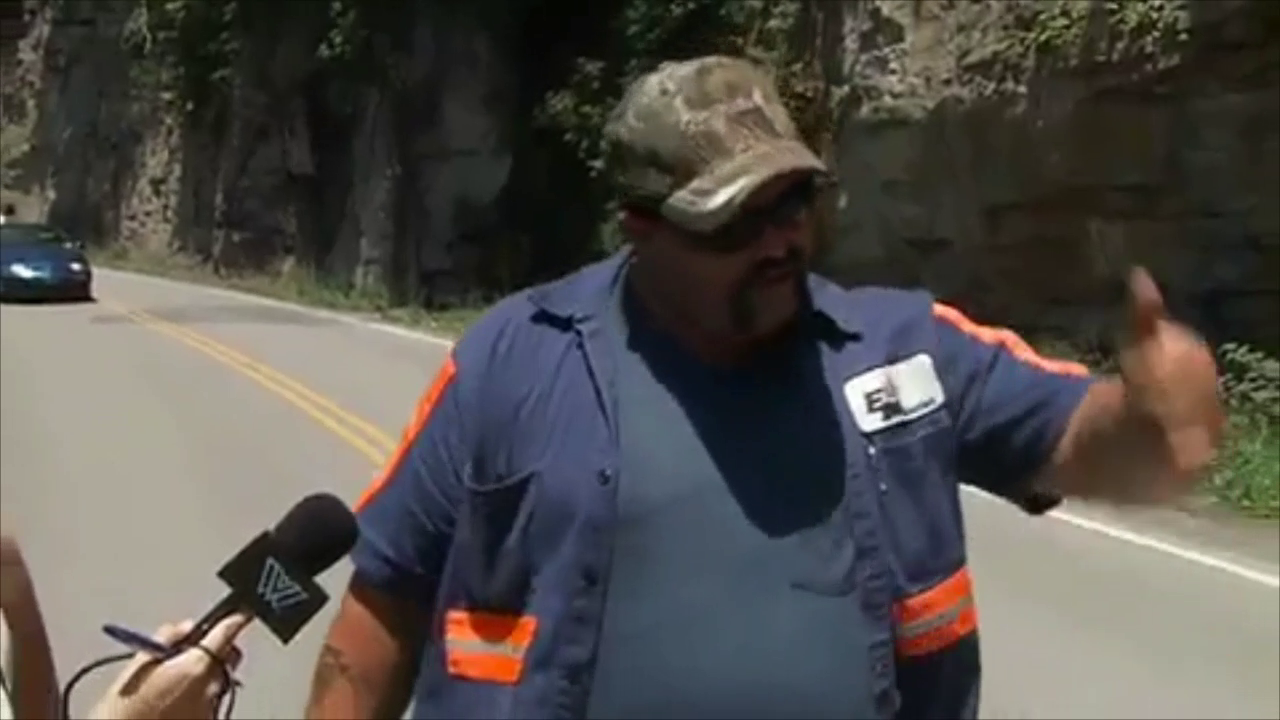
\includegraphics[width=4.2cm]{Figures/mmCult5/frame103.png} & 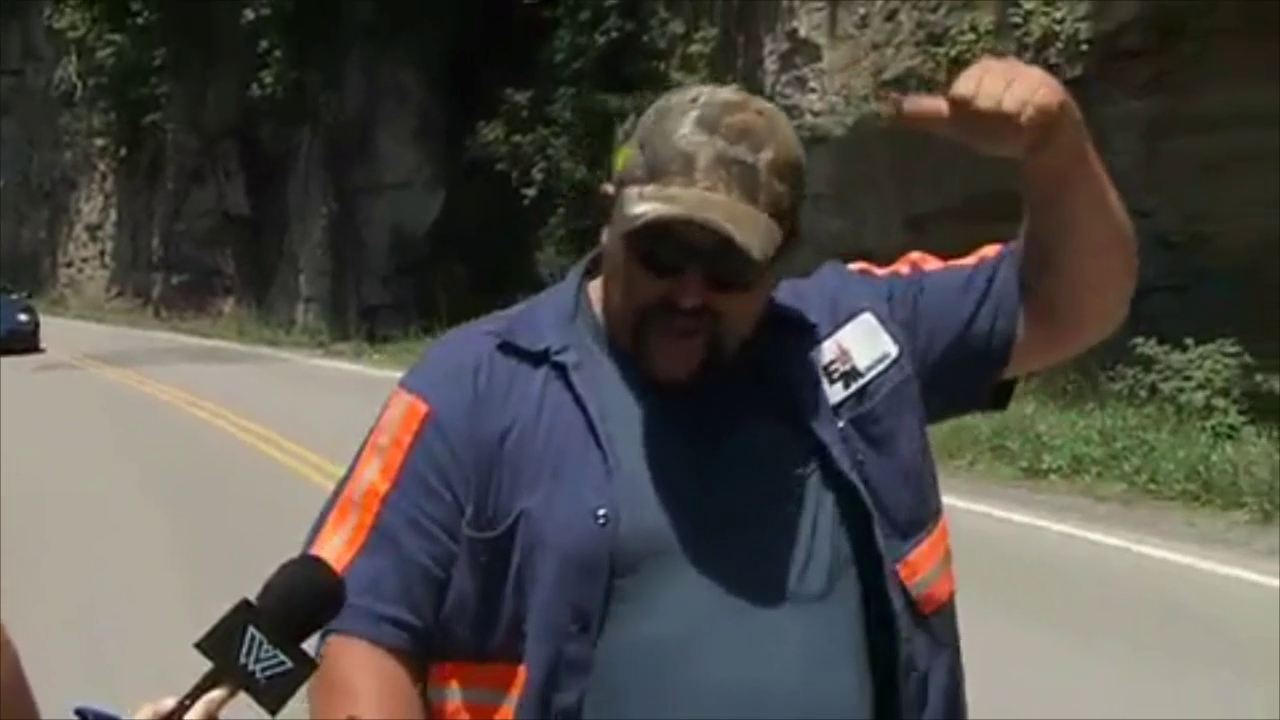
\includegraphics[width=4.2cm]{Figures/mmCult5/frame118.png}  

\end{tabular}
\caption{Cultural Level - Example 5}
\begin{footnotesize}

\end{footnotesize}
\label{fig:figure1}
\end{figure}

\section{Socio-Economic Level}

\subsection{Socio-Economic Level - Example 1}


\begin{footnotesize}

Source: \url{https://www.youtube.com/embed/gU7PBoy-wFE?start=10&end=21}\\
\textit{Embeded videos require Adobe Flash.}
\begin{center}
\includemedia[width=9.60cm,height=5.40cm,activate=pageopen,
passcontext,
transparent,
addresource=Figures/06.mp4,
flashvars={source=Figures/06.mp4}
]{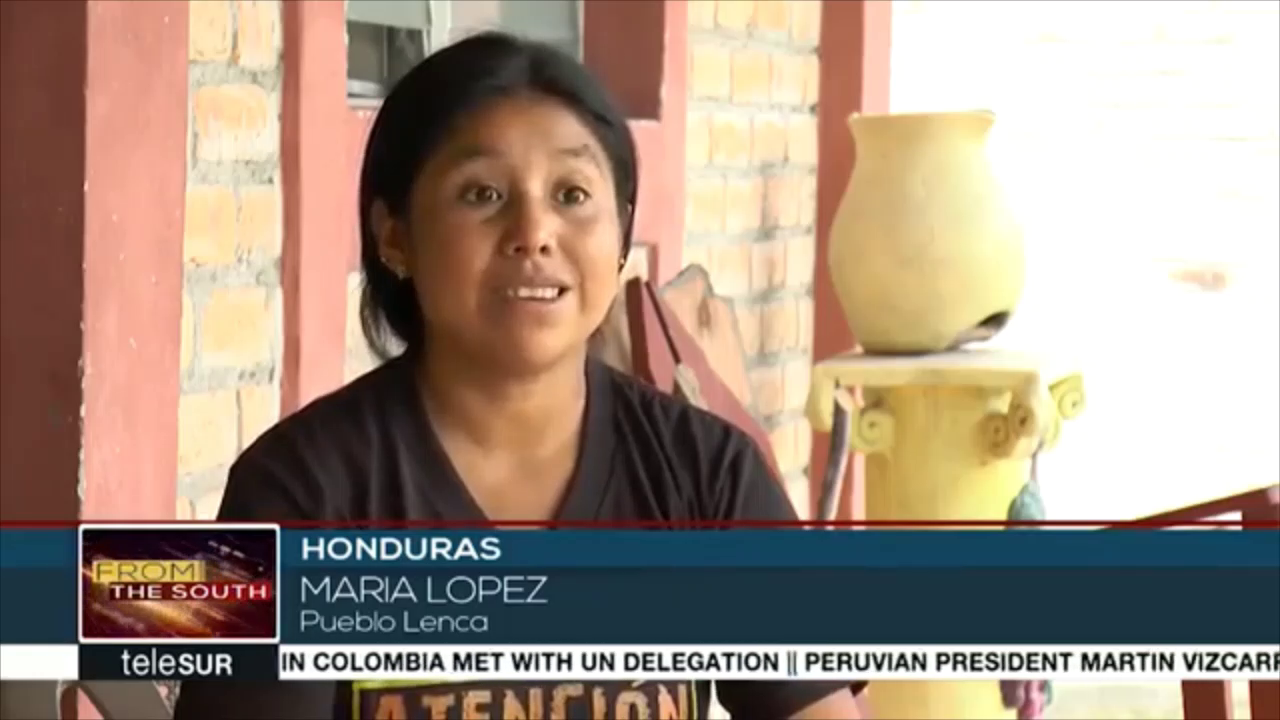
\includegraphics{Figures/mmEcon/frame304.png}}{VPlayer.swf}
\end{center}
\end{footnotesize}

\begin{footnotesize}
\texttt{(Translated from Spanish - only gesture annotation)
The worst impacts have been state violence. Why? Because we have comrades who have been killed following military harassment. [We've already lost one person].\textsuperscript{1}}
\end{footnotesize}

\begin{footnotesize}
\begin{enumerate}
   \item Raised eyebrows; wide eyes; extenuated blinks
\end{enumerate}
\end{footnotesize}

\begin{figure}[H]
\centering
\begin{tabular}{llll}
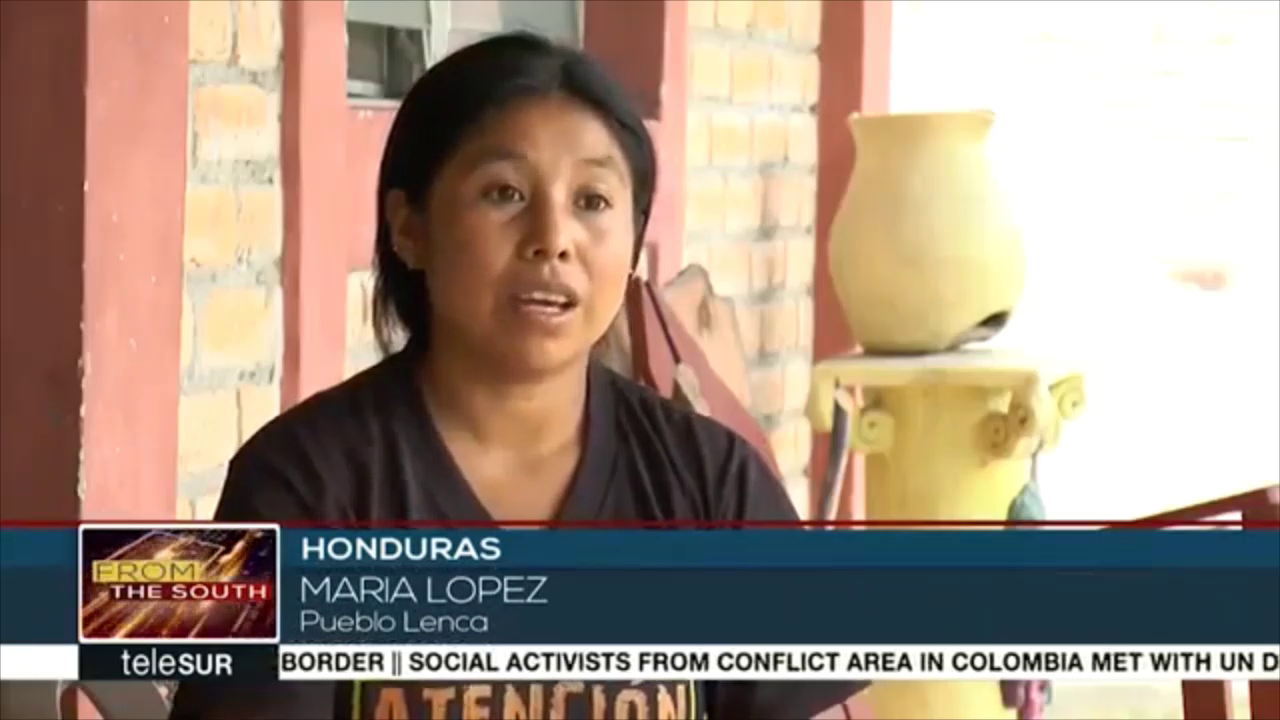
\includegraphics[width=4.2cm]{Figures/mmEcon/frame66.png} & 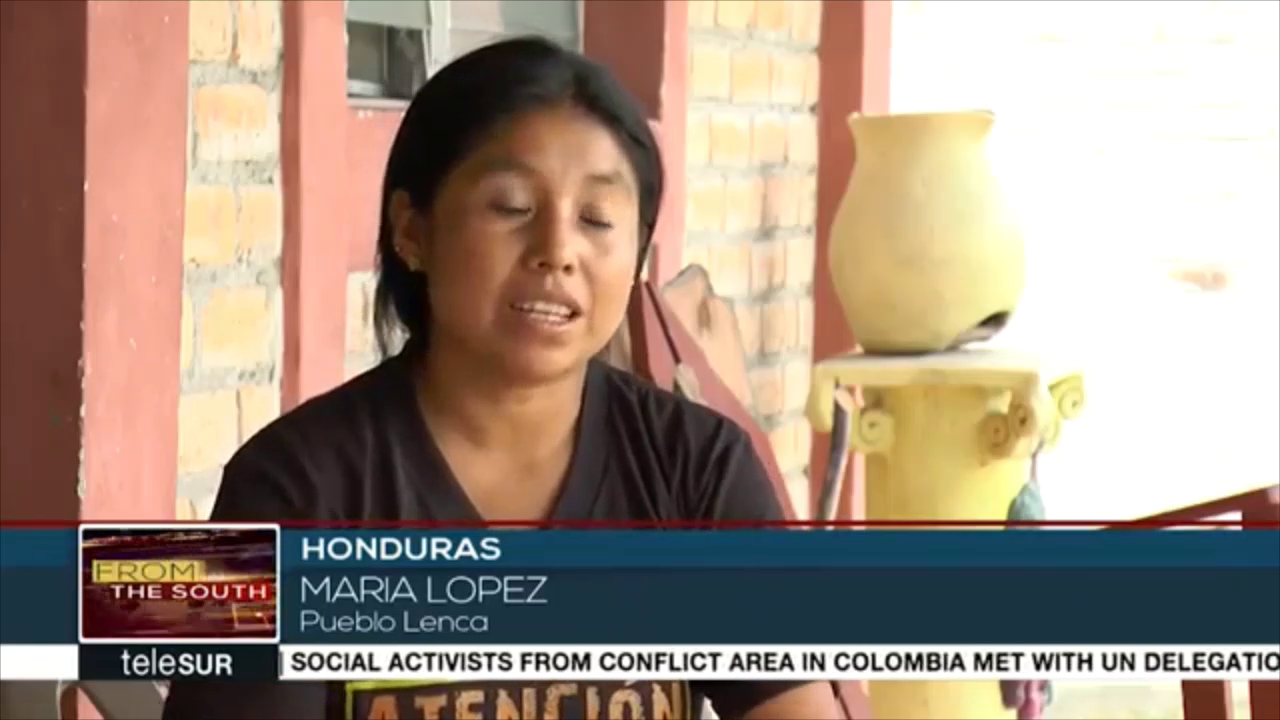
\includegraphics[width=4.2cm]{Figures/mmEcon/frame110.png} & 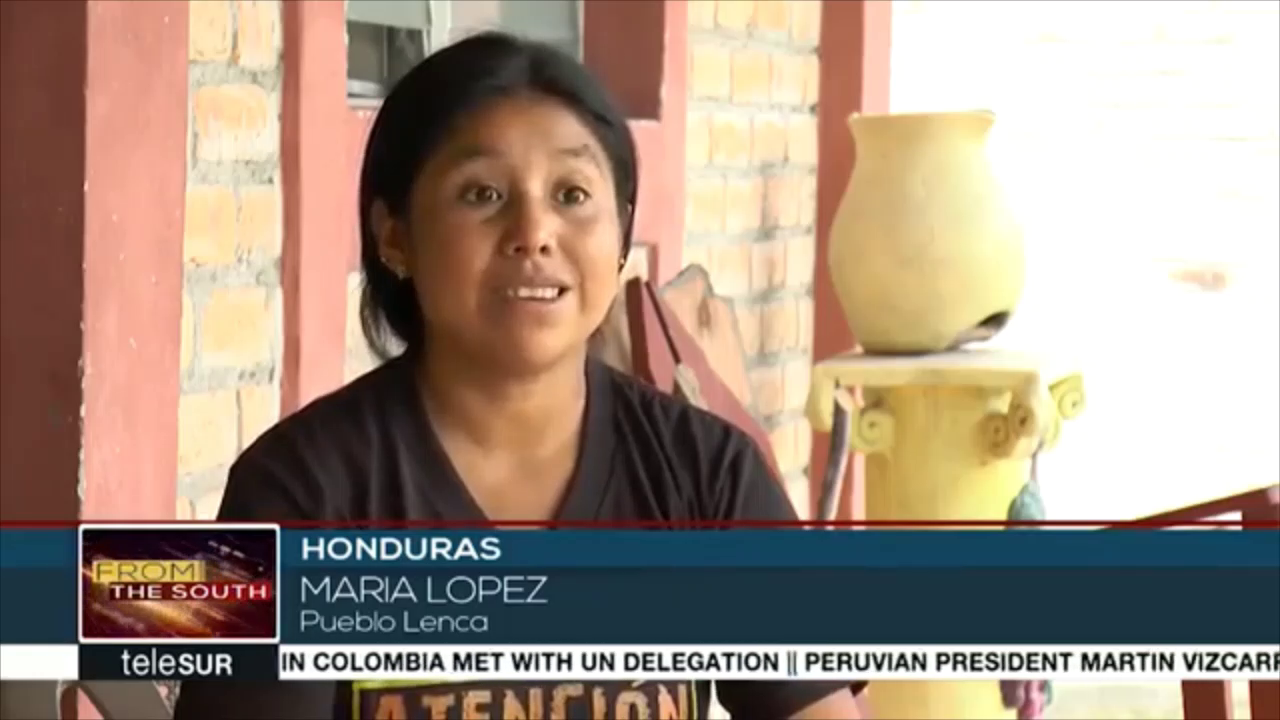
\includegraphics[width=4.2cm]{Figures/mmEcon/frame304.png}  
\end{tabular}
\caption{Socio-Economic level - Example 1}
\begin{footnotesize}

\end{footnotesize}
\label{fig:figure1}
\end{figure}





\subsection{Socio-Economic Level - Example 2}

\begin{footnotesize}
Source: \url{https://www.youtube.com/embed/Sh0_Wf8F4RM?start=390&end=420}\\
\textit{Embeded videos require Adobe Flash.}
\begin{center}
\includemedia[width=9.60cm,height=5.40cm,activate=pageopen,
passcontext,
transparent,
addresource=Figures/11.mp4,
flashvars={source=Figures/11.mp4}
]{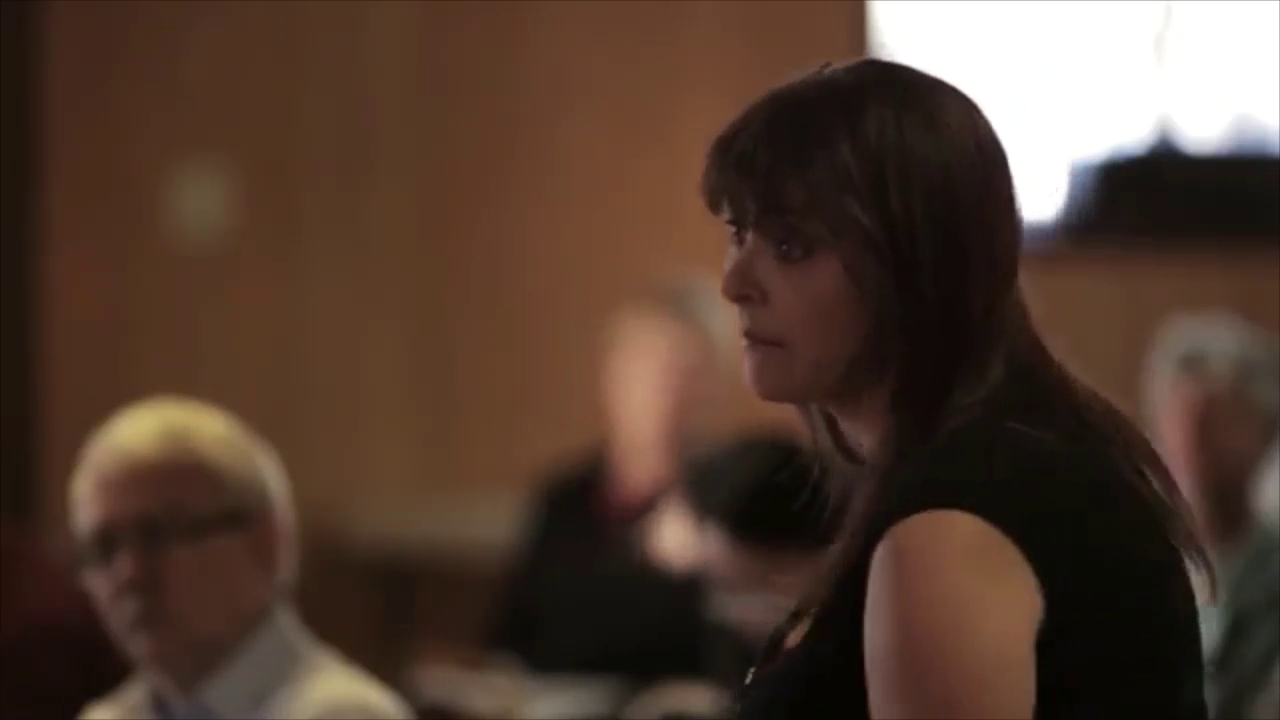
\includegraphics{Figures/mmEcon1/frame988.png}}{VPlayer.swf}
\end{center}
\end{footnotesize}



\begin{footnotesize}

\texttt{<\annotate{Five years} we'e been trying to keep our doors open, \annotate{thinking} (.) any day now> those jobs were going to be here. >These are the only people that have come in and offered us jobs$\uparrow$< If \annotate{any} of the people here who are against it had come in and [said they had jobs to match it, we'd be behind that too. But right now this is all we've got]\textsuperscript{1}. Everyone one of you who has stood up against this could have brought in jobs [for \annotate{us}.]\textsuperscript{2}}
\end{footnotesize}

\begin{footnotesize}
\begin{enumerate}
   \item Raised and upward slanted eyebrows, stressed blink
   \item Hand points inwards toward chest; index finger extended
\end{enumerate}
\end{footnotesize}

\begin{figure}[H]
\centering
\begin{tabular}{llll}
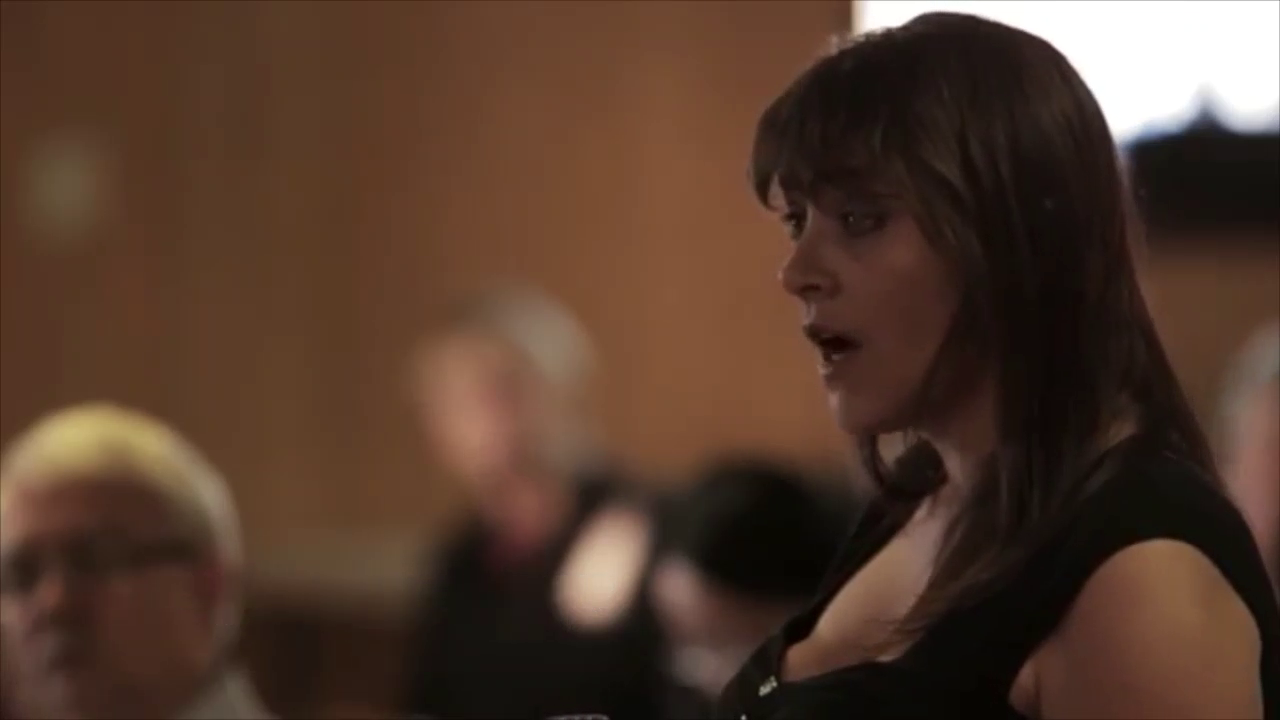
\includegraphics[width=4.2cm]{Figures/mmEcon1/frame413.png} & 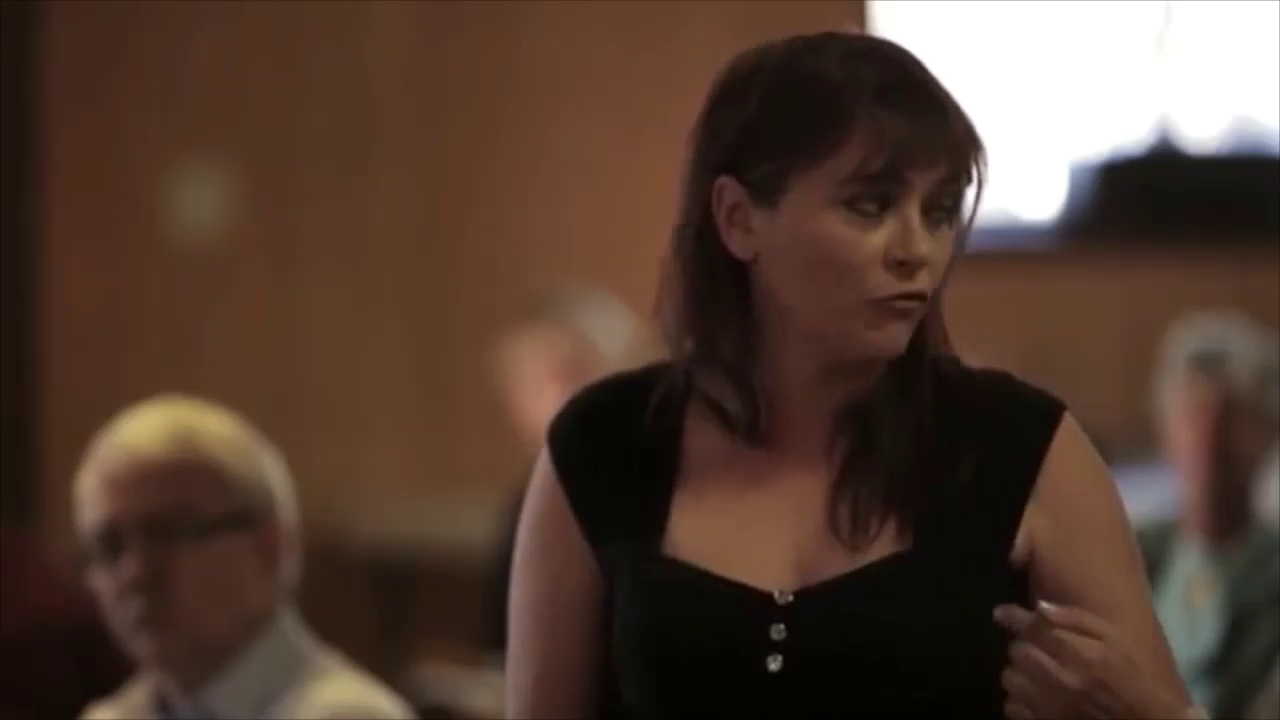
\includegraphics[width=4.2cm]{Figures/mmEcon1/frame725.png} & 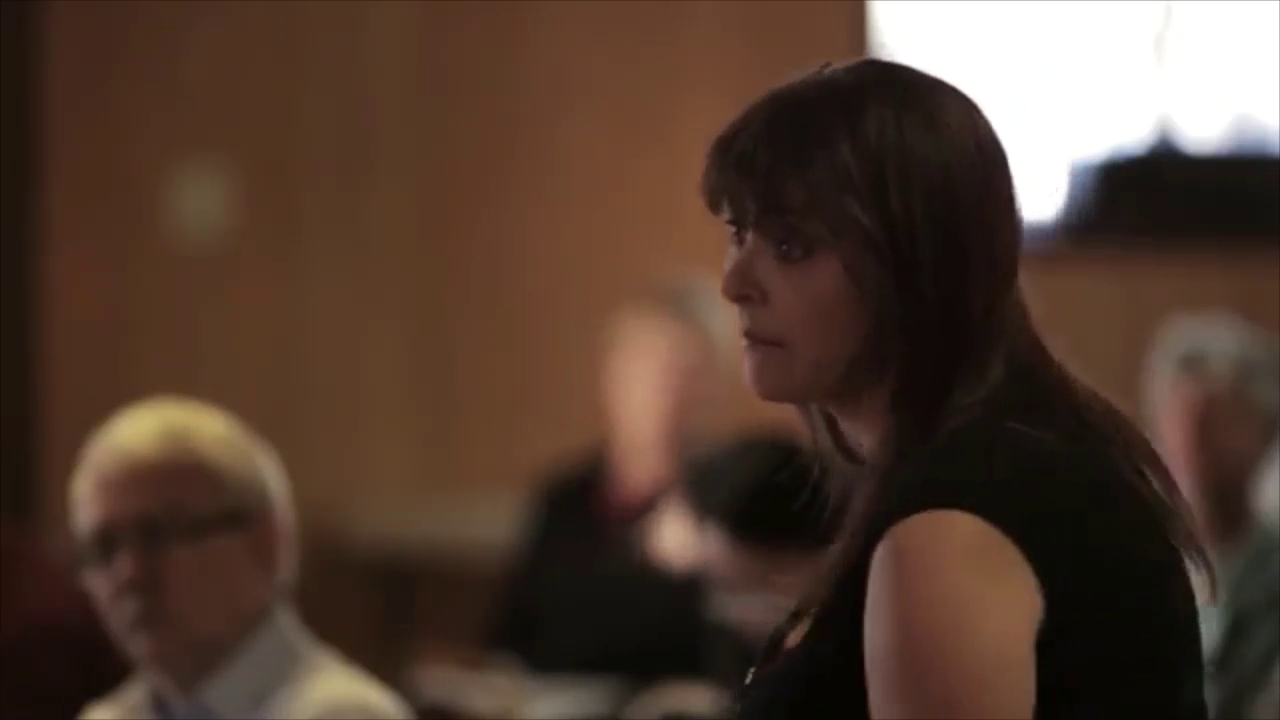
\includegraphics[width=4.2cm]{Figures/mmEcon1/frame988.png}  
\end{tabular}
\caption{Socio-Economic level - Example 2}
\begin{footnotesize}

\end{footnotesize}
\label{fig:figure1}
\end{figure}

\begin{figure}[H]
\centering
\begin{tabular}{llll}
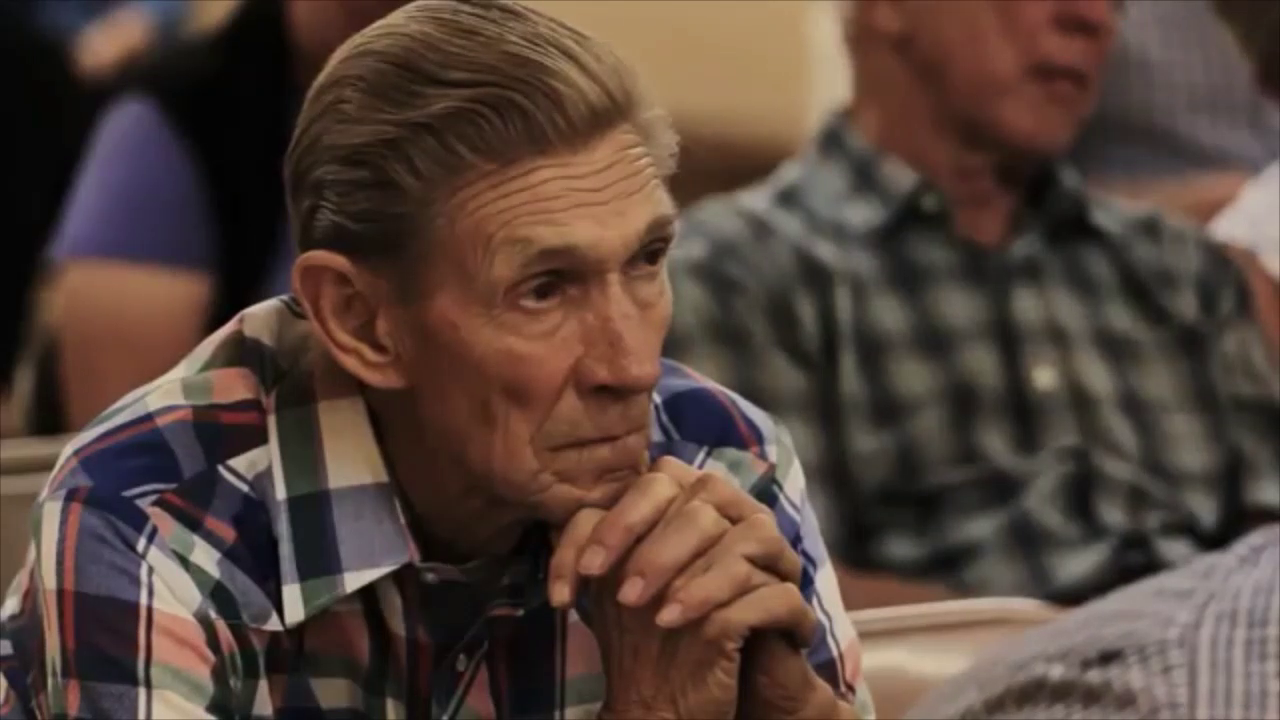
\includegraphics[width=5cm]{Figures/mmEcon2/frame137.png} &  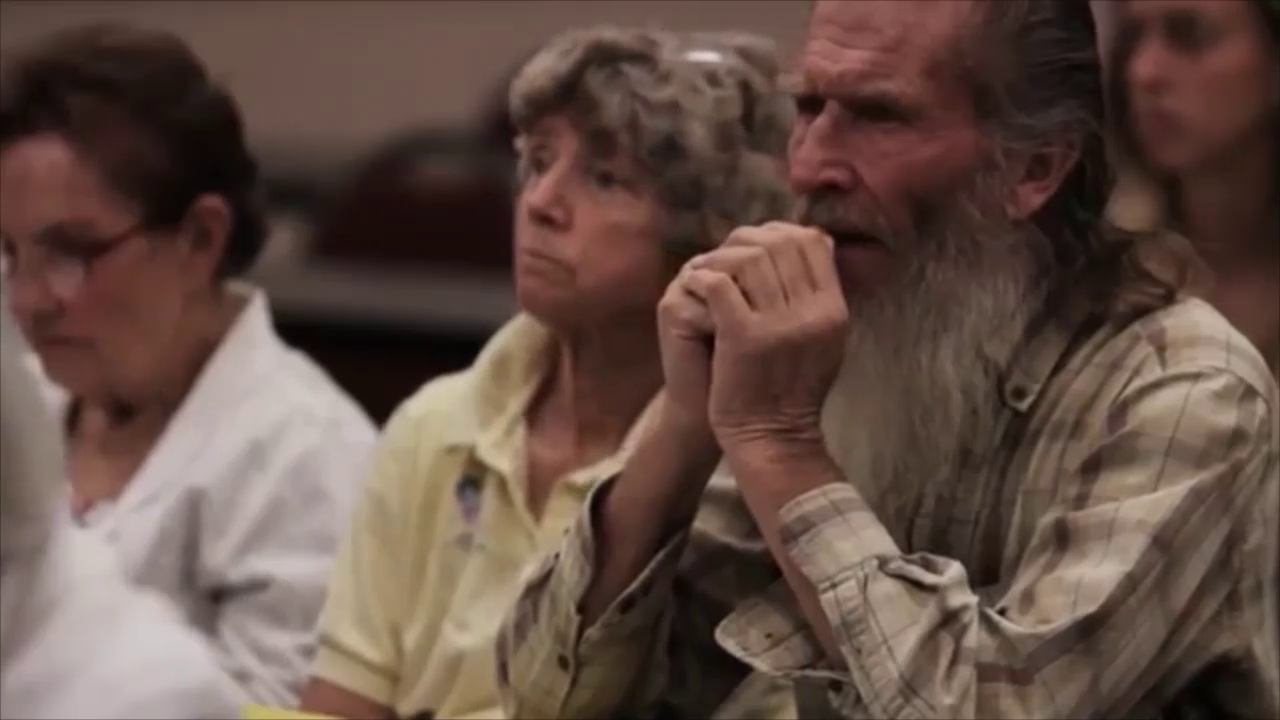
\includegraphics[width=5cm]{Figures/mmEcon2/frame222.png} \\

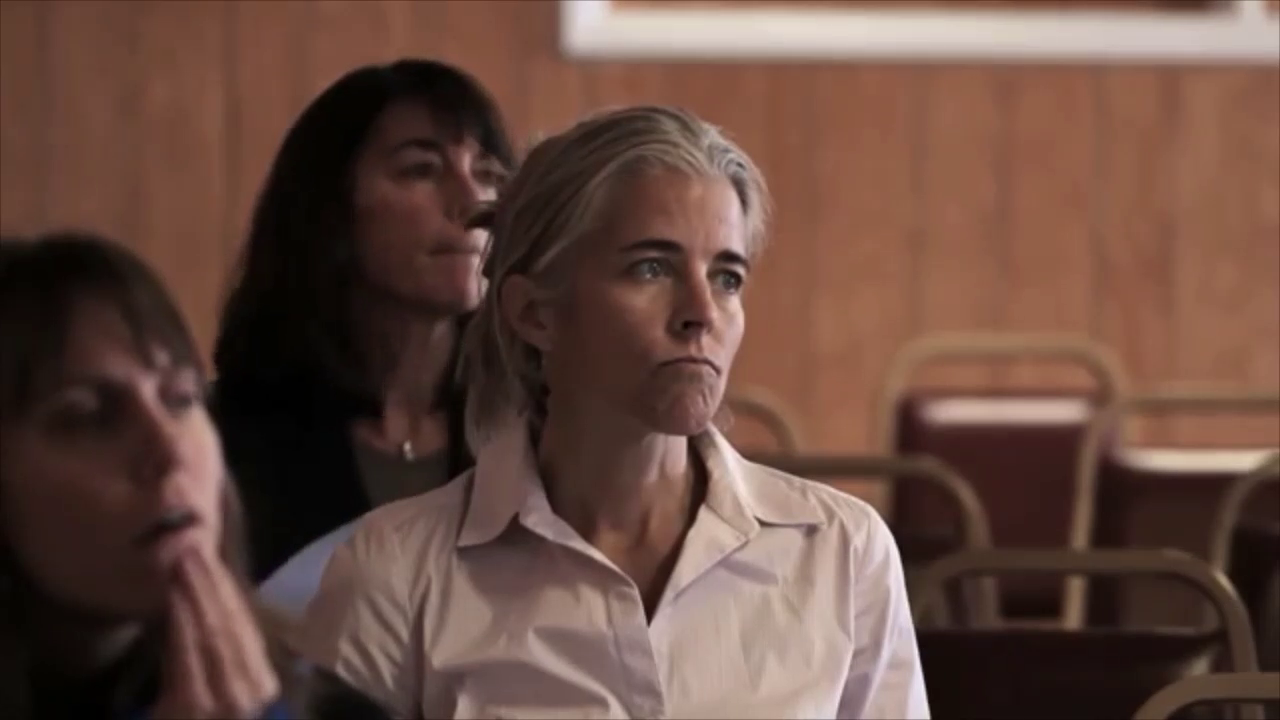
\includegraphics[width=5cm]{Figures/mmEcon2/frame529.png} & 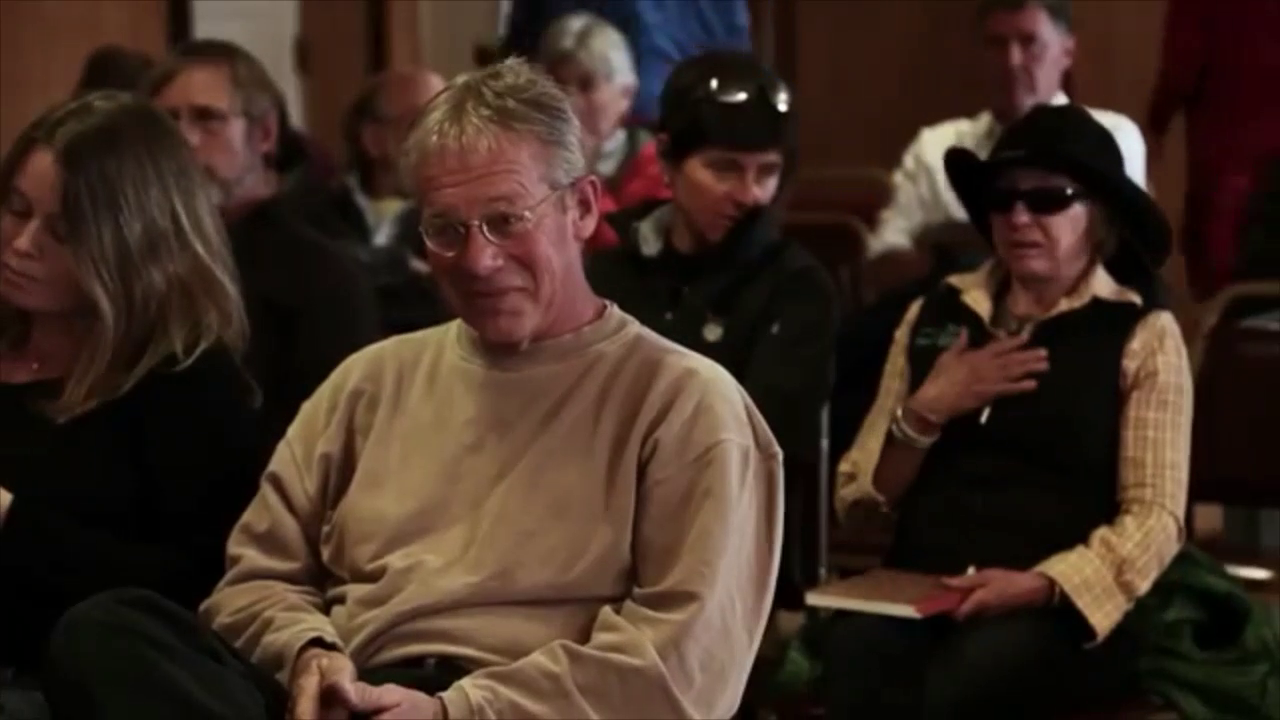
\includegraphics[width=5cm]{Figures/mmEcon2/frame857.png}  

\end{tabular}
\caption{Socio-economic level, listener reactions}
\label{fig:figure1}
\end{figure}




















\subsection{Socio-Economic Level - Example 3}


\begin{footnotesize}

Source: \url{https://www.youtube.com/embed/vBhvFWRLiOs?start=1299&end=1316}\\
\textit{Embeded videos require Adobe Flash.}
\begin{center}
\includemedia[width=9.60cm,height=5.40cm,activate=pageopen,
passcontext,
transparent,
addresource=Figures/19.mp4,
flashvars={source=Figures/19.mp4}
]{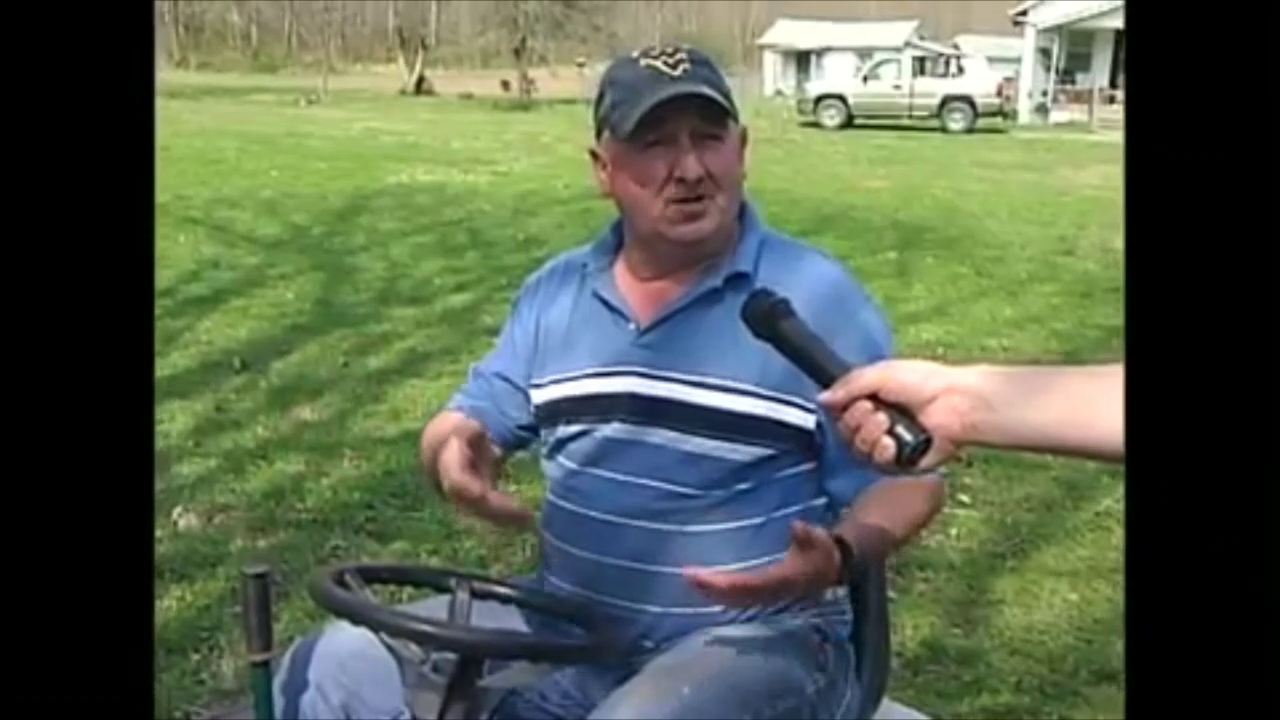
\includegraphics{Figures/mmEcon3/frame610.png}}{VPlayer.swf}
\end{center}
\end{footnotesize}



\begin{footnotesize}
\texttt{[They're fighting]\textsuperscript{1} a losing battle I feel (.) myself I feel like they're just fighting a losing battle, because the <[\annotate{politicians}]\textsuperscript{2} and the [\annotate{big} coal companies and things> \annotate{they're} going to win hands down >because the judges and arbitrators are just going to go their way.<]\textsuperscript{3} }
\end{footnotesize}

\begin{footnotesize}
\begin{enumerate}
   \item Both hands extend outward, palms up
   \item Both hands motion forward/downward, palms down
   \item Both hands extend outward, palms up, with emphasis
\end{enumerate}
\end{footnotesize}

\begin{figure}[H]
\centering
\begin{tabular}{llll}
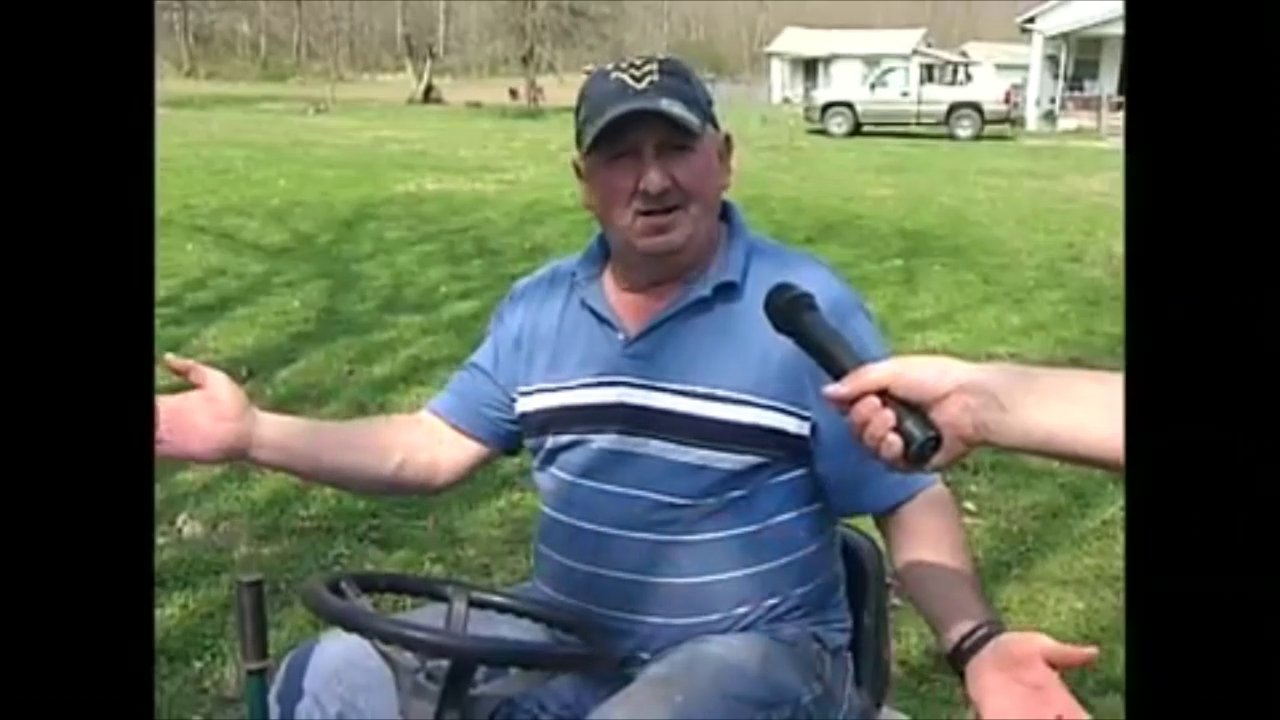
\includegraphics[width=4.2cm]{Figures/mmEcon3/frame189.png} & 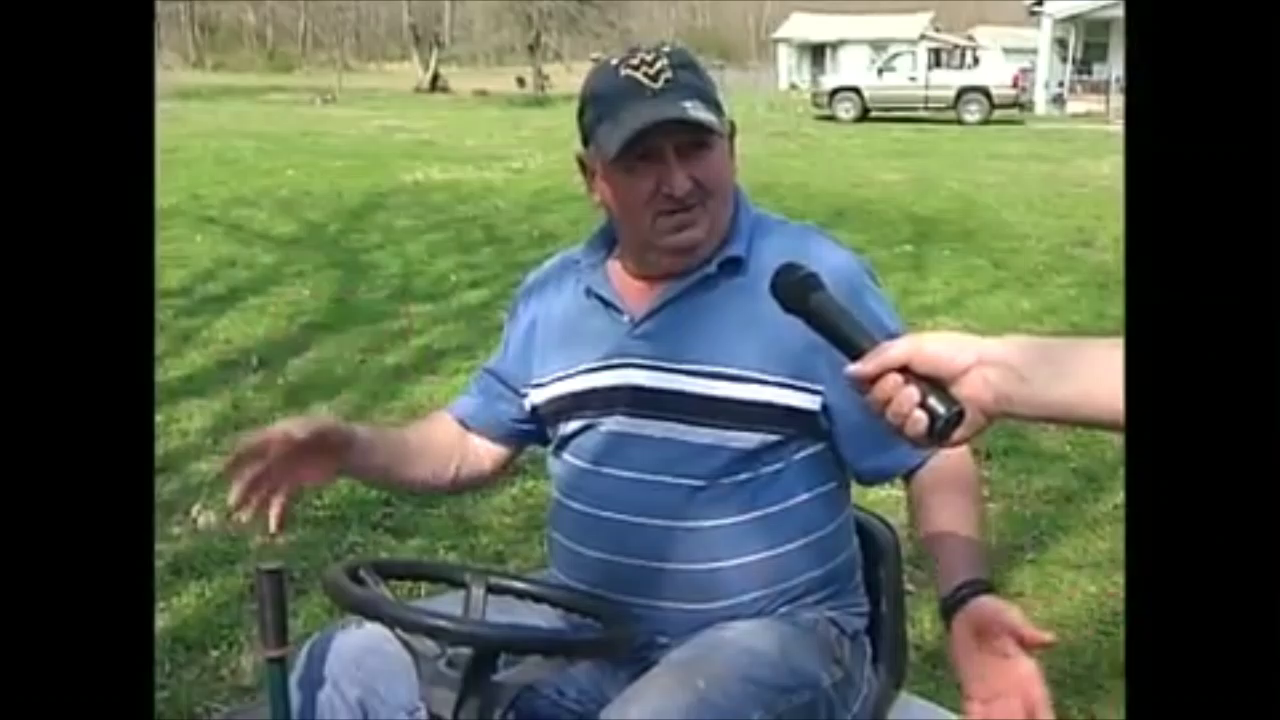
\includegraphics[width=4.2cm]{Figures/mmEcon3/frame450.png} & 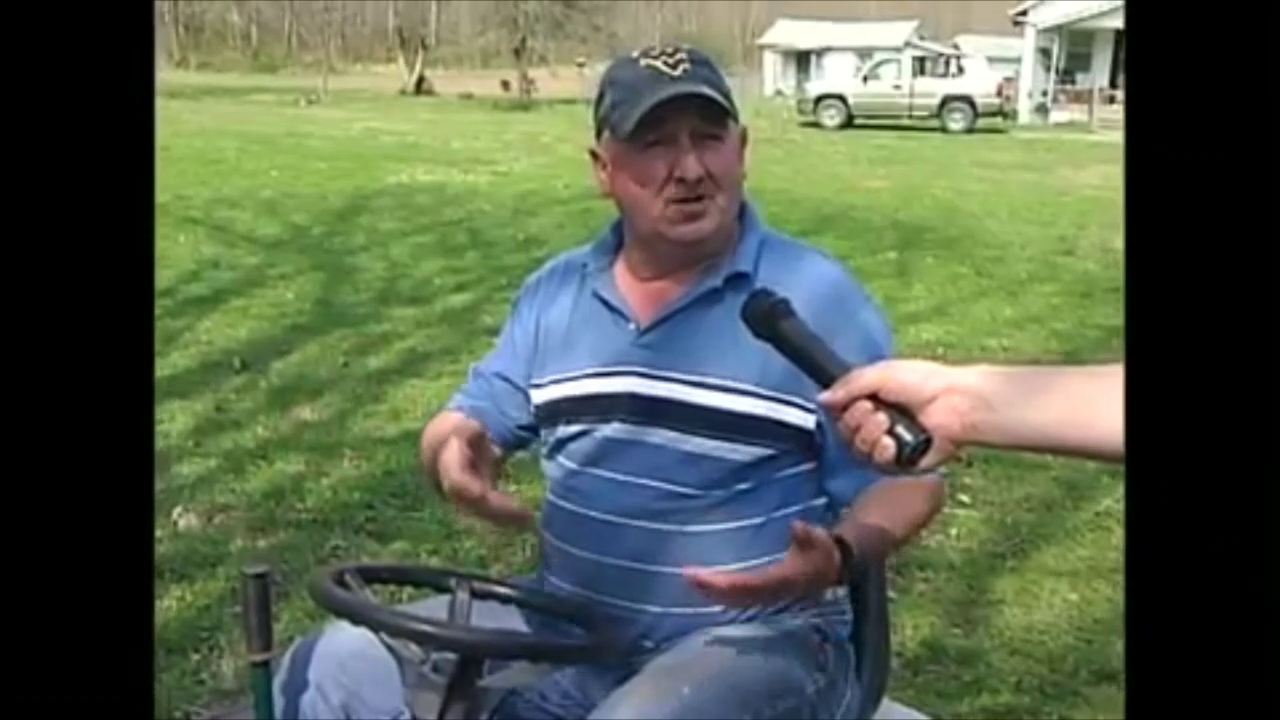
\includegraphics[width=4.2cm]{Figures/mmEcon3/frame610.png}  
\end{tabular}
\caption{Socio-Economic Level - Example 3}
\begin{footnotesize}

\end{footnotesize}
\label{fig:figure1}
\end{figure}









\subsection{Socio-Economic Level - Example 4}

\begin{footnotesize}

Source: \url{https://www.youtube.com/embed/vBhvFWRLiOs?start=58&end=75}\\
\textit{Embeded videos require Adobe Flash.}
\begin{center}
\includemedia[width=9.60cm,height=5.40cm,activate=pageopen,
passcontext,
transparent,
addresource=Figures/16.mp4,
flashvars={source=Figures/16.mp4}
]{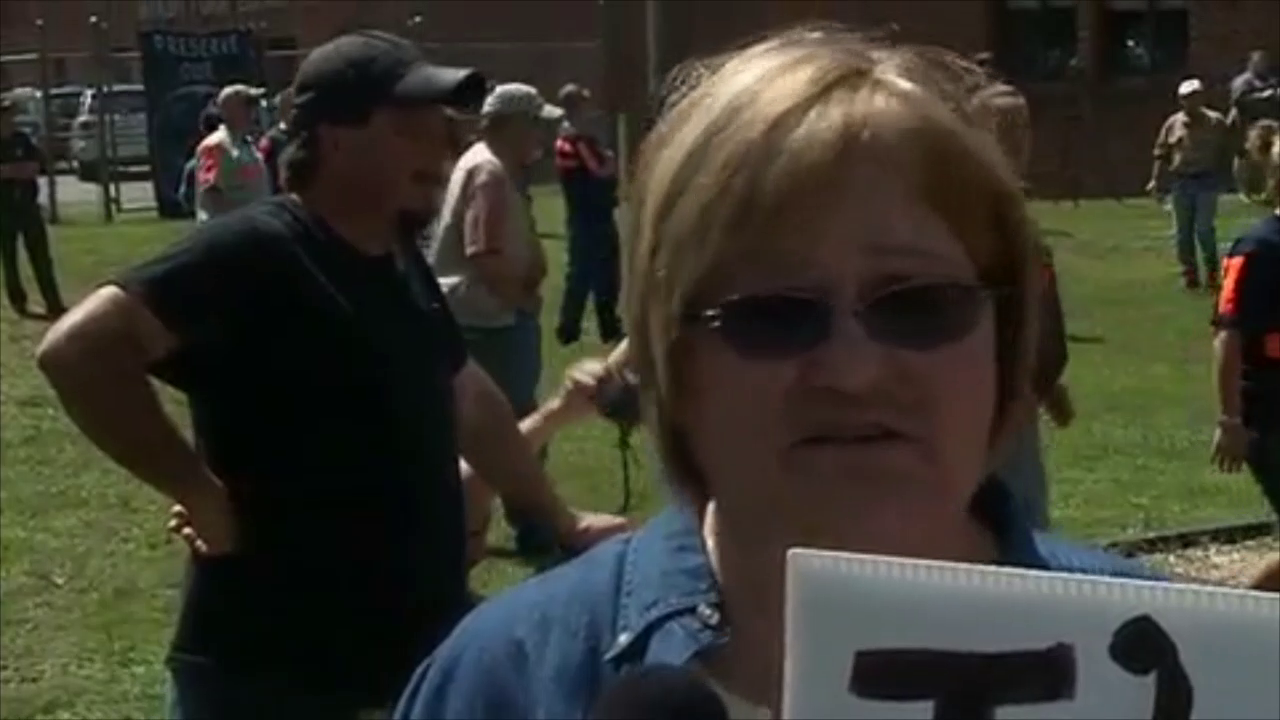
\includegraphics{Figures/mmEcon4/frame3.png}}{VPlayer.swf}
\end{center}
\end{footnotesize}


\begin{footnotesize}
\texttt{If you choose to live in West Virginia, [this is (.) this is the best paying job there is$\uparrow$]\textsuperscript{1}. \textit{Interviewer}: What happens if mountain top removal goes away, what happens to you and your family? \annotate{WE GO HUNGRY!}\textsuperscript{2}}

\end{footnotesize}

\begin{footnotesize}
\begin{enumerate}
   \item Shoulders raise; nodding
   \item Eyebrows raise
\end{enumerate}
\end{footnotesize}

\begin{figure}[H]
\centering
\begin{tabular}{llll}
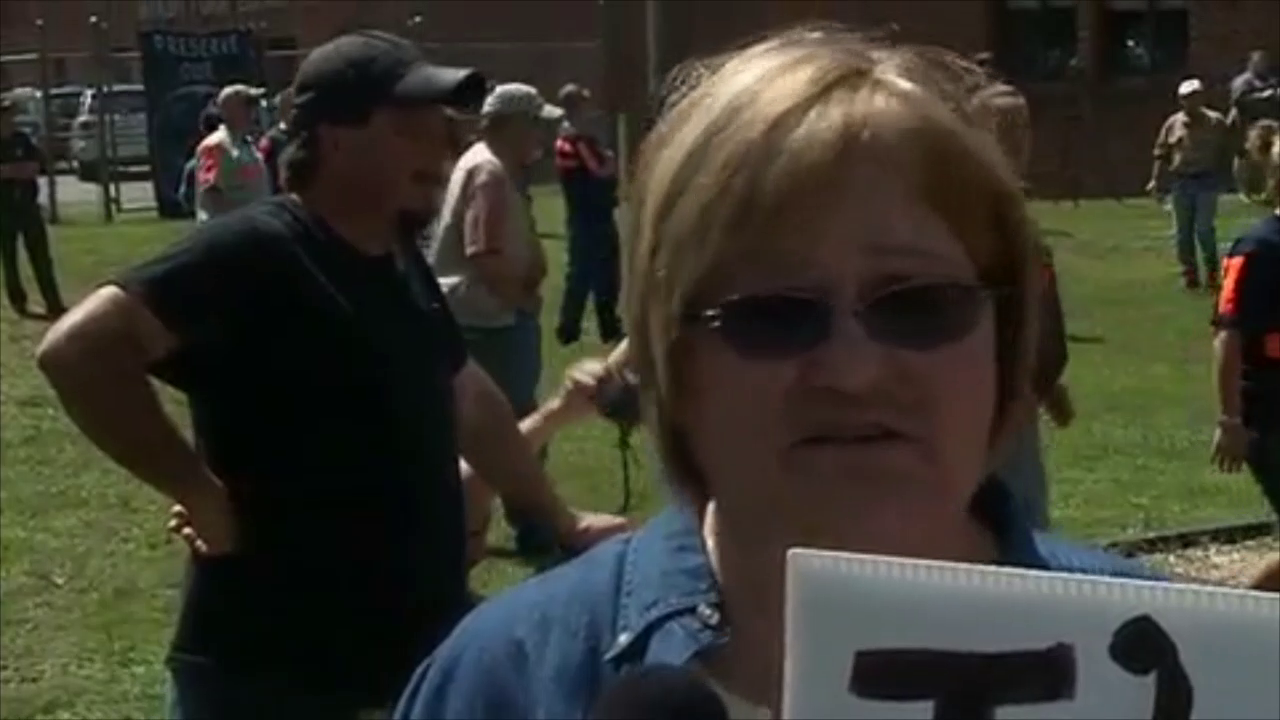
\includegraphics[width=4.2cm]{Figures/mmEcon4/frame3.png} & 
\includegraphics[width=4.2cm]{Figures/mmEcon4/frame551.png} & 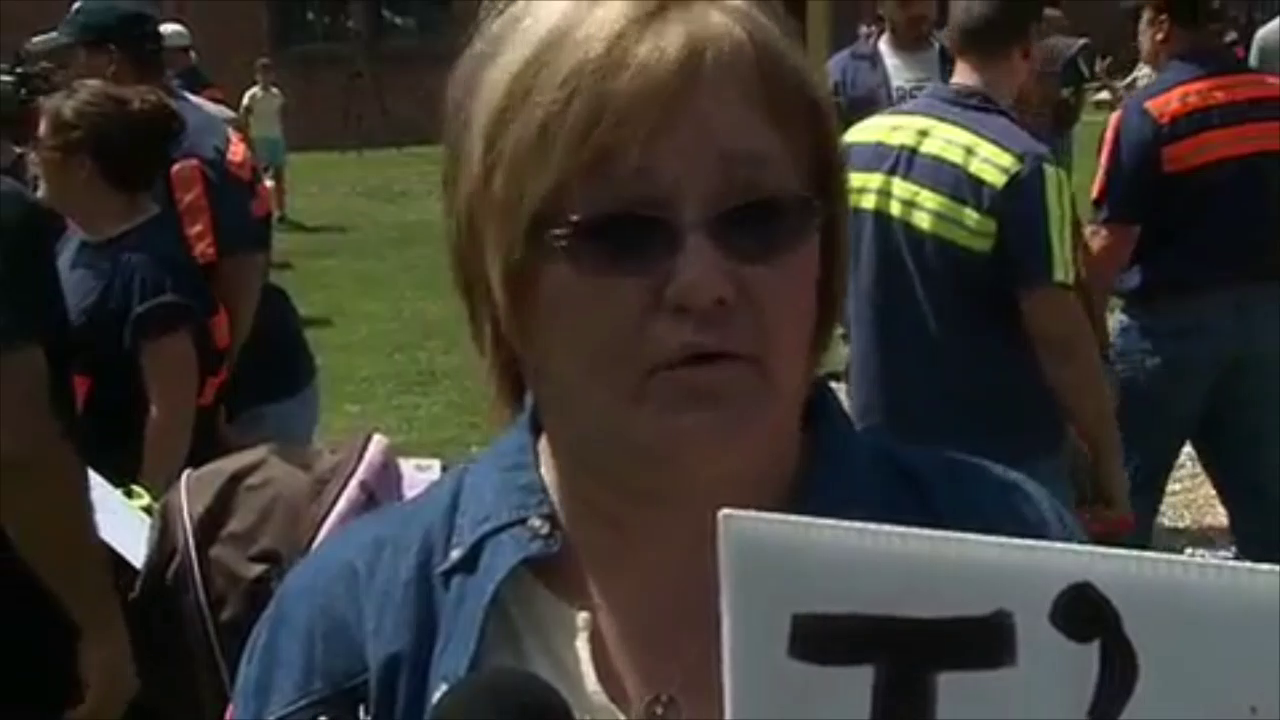
\includegraphics[width=4.2cm]{Figures/mmEcon4/frame901.png}  
\end{tabular}
\caption{Socio-Economic level - Example 4}
\begin{footnotesize}

\end{footnotesize}
\label{fig:figure1}
\end{figure} % Appendix C

\addtocontents{toc}{\vspace{2em}}  % Add a gap in the Contents, for aesthetics
\backmatter

%% ----------------------------------------------------------------
\label{Bibliography}
\lhead{\textit{Bibliography}}  % Change the left side page header to "Bibliography"
\normalem
\bibliographystyle{apalike}  % Use the "unsrtnat" BibTeX style for formatting the Bibliography
\bibliography{Bibliography}  % The references (bibliography) information are stored in the file named "Bibliography.bib"
\end{document}  % The End
%% ----------------------------------------------------------------